% !TeX spellcheck = en_US
\documentclass{article}

% Pass options to natbib
\PassOptionsToPackage{numbers, compress}{natbib}

% NeurIPS packages
\usepackage[]{neurips_2023}
\usepackage[utf8]{inputenc} % allow utf-8 input
\usepackage[T1]{fontenc}    % use 8-bit T1 fonts
%\usepackage{hyperref}       % hyperlinks
\usepackage{url}            % simple URL typesetting
\usepackage{booktabs}       % professional-quality tables
\usepackage{amsfonts}       % blackboard math symbols
\usepackage{nicefrac}       % compact symbols for 1/2, etc.
\usepackage{microtype}      % microtypography
\usepackage{xcolor}         % colors

% Redefine paragraph to be tighter
\renewcommand{\paragraph}[1]{{\bf #1}~~}

% Array/table packages
\usepackage{tabularx}
\usepackage{array,multirow}
\usepackage{colortbl}
\newcommand{\PreserveBackslash}[1]{\let\temp=\\#1\let\\=\temp}
\newcolumntype{C}[1]{>{\PreserveBackslash\centering}p{#1}}
\newlength{\tblw}

% Latin
\usepackage{xspace}
\newcommand{\eg}{\textit{e.g.\@}\xspace}
\newcommand{\ie}{\textit{i.e.\@}\xspace}
\newcommand{\cf}{\textit{cf.\@}\xspace}
\newcommand{\etc}{\textit{etc.\@}\xspace}
\newcommand{\etal}{\textit{et~al.\@}\xspace}

% Our method
\newcommand{\our}{\textsc{sfr}\xspace}

% Tikz
\usepackage{tikz}
\usepackage{pgfplots}
\usetikzlibrary{patterns}
\usetikzlibrary{decorations,backgrounds,arrows.meta,calc}
\usetikzlibrary{shapes,arrows,positioning}

% Appendix/supplement title
\newcommand{\nipstitle}[1]{{%
    % rules for title box at top and bottom
    \def\toptitlebar{\hrule height4pt \vskip .25in \vskip -\parskip} 
    \def\bottomtitlebar{\vskip .29in \vskip -\parskip \hrule height1pt \vskip .09in} 
    \phantomsection\hsize\textwidth\linewidth\hsize%
    \vskip 0.1in%
    \toptitlebar%
    \begin{minipage}{\textwidth}%
        \centering{\LARGE\bf #1\par}%
    \end{minipage}%
    \bottomtitlebar%
    \addcontentsline{toc}{section}{#1}%
}}

% Bibliography
%\usepackage[maxcitenames=1, maxbibnames=4, doi=false, isbn=false, eprint=true, backend=bibtex, hyperref=true, url=false, style=authoryear-comp]{biblatex}
%\addbibresource{zotero-library.bib}
% \addbibresource{paper/zotero-library.bib}

% Let's use good old bibtex instead

% Figure customization: Tight legend box
\pgfplotsset{every axis/.append style={
		legend style={inner xsep=1pt, inner ysep=0.5pt, nodes={inner sep=1pt, text depth=0.1em},draw=none,fill=none}
}}

% Our packages
\usepackage{todonotes}
\usepackage[colorlinks=true,linkcolor=black,allcolors=black,urlcolor=black,citecolor=black]{hyperref}
\usepackage{amsmath}
\usepackage{bm}
\usepackage{algpseudocode}
\usepackage{algorithm}
\usepackage{derivative}
\usepackage{wrapfig}

\usepackage{tikz,pgfplots}
\usepackage{subcaption}
\usetikzlibrary{}

\newcommand{\defeq}{\vcentcolon=}

% Definitions/assumptions etc
\usepackage{mathtools}
\newtheorem{definition}{Definition}[section]
\newtheorem{assumption}{Assumption}[section]
\newtheorem{theorem}{Theorem}[section]
\newtheorem{lemma}{Lemma}[section]
% \newtheorem*{remark}{Remark}

% Short commands for commonly used stuff
\DeclareMathOperator{\R}{\mathbb{R}}
\DeclareMathOperator{\E}{\mathbb{E}}
\DeclareMathOperator{\V}{\mathbb{V}}


% Short section names etc
% This must be imported last!
%\usepackage{cleveref}
\usepackage[capitalise,nameinlink]{cleveref}
\crefname{section}{Sec.}{Secs.}
\crefname{algorithm}{Alg.}{Algs.}
\crefname{appendix}{App.}{Apps.}
\crefname{definition}{Def.}{Defs.}
\crefname{table}{Table}{Tables}

% Config for Arno's awesome TikZ plotting stuff
\newlength{\figurewidth}
\newlength{\figureheight}


% Variables
\newcommand{\state}{\ensuremath{\mathbf{s}}}
\newcommand{\action}{\ensuremath{\mathbf{a}}}
\newcommand{\noise}{\ensuremath{\bm\epsilon}}
\newcommand{\discount}{\ensuremath{\gamma}}
\newcommand{\inducingInput}{\ensuremath{\mathbf{Z}}}
\newcommand{\inducingVariable}{\ensuremath{\mathbf{u}}}
\newcommand{\dataset}{\ensuremath{\mathcal{D}}}
\newcommand{\dualParam}[1]{\ensuremath{\bm{\lambda}_{#1}}}
\newcommand{\meanParam}[1]{\ensuremath{\bm{\mu}_{#1}}}

% Indexes
\newcommand{\horizon}{\ensuremath{h}}
\newcommand{\Horizon}{\ensuremath{H}}
\newcommand{\numDataNew}{\ensuremath{N^{\text{new}}}}
\newcommand{\numDataOld}{\ensuremath{N^{\text{old}}}}
\newcommand{\numInducing}{\ensuremath{M}}

% Domains
\newcommand{\stateDomain}{\ensuremath{\mathcal{S}}}
\newcommand{\actionDomain}{\ensuremath{\mathcal{A}}}
\newcommand{\inputDomain}{\ensuremath{\mathbb{R}^{D}}}
\newcommand{\outputDomain}{\ensuremath{\mathbb{R}^{C}}}
\newcommand{\policyDomain}{\ensuremath{\Pi}}

% Functions
\newcommand{\rewardFn}{\ensuremath{r}}
\newcommand{\transitionFn}{\ensuremath{f}}
\newcommand{\latentFn}{\ensuremath{f}}

\newcommand{\optimisticTransition}{\ensuremath{\hat{f}}}
\newcommand{\optimisticTransitionMean}{\ensuremath{\mu_{\optimisticTransition}}}
\newcommand{\optimisticTransitionCov}{\ensuremath{\mu_{\optimisticTransition}}}
\newcommand{\optimisticTransitionSet}{\ensuremath{\mathcal{M}}}


% Parameters
% \newcommand{\weights}{\ensuremath{\bm\phi}}
\newcommand{\weights}{\ensuremath{\mathbf{w}}}
\newcommand{\valueFnParams}{\ensuremath{\psi}}
\newcommand{\policyParams}{\ensuremath{\theta}}

% Networks
\newcommand{\transitionFnWithParams}{\ensuremath{\transitionFn_{\weights}}}
\newcommand{\valueFn}{\ensuremath{\mathbf{Q}}}
\newcommand{\stateValueFn}{\ensuremath{\mathbf{V}}}
% \newcommand{\valueFn}{\ensuremath{\mathbf{Q}_{\valueFnParams}}}
\newcommand{\policy}{\ensuremath{\pi}}
\newcommand{\pPolicy}{\ensuremath{\pi_{\policyParams}}}


% Packages for bold math
\usepackage{bm}
\newcommand{\mathbold}[1]{\bm{#1}}
\newcommand{\mbf}[1]{\mathbf{#1}}
\renewcommand{\mid}{\,|\,}


% Math Macros
\newcommand{\MB}{\mbf{B}}
\newcommand{\MC}{\mbf{C}}
\newcommand{\MZ}{\mbf{Z}}
\newcommand{\MV}{\mbf{V}}
\newcommand{\MX}{\mbf{X}}
\newcommand{\MA}{\mbf{A}}
\newcommand{\MK}{\mbf{K}}
\newcommand{\MI}{\mbf{I}}
\newcommand{\MH}{\mbf{H}}
\newcommand{\T}{\top}
\newcommand{\vzeros}{\mbf{0}}
\newcommand{\vtheta}[0]{\mathbold{\theta}}
\newcommand{\valpha}[0]{\mathbold{\alpha}}
\newcommand{\vkappa}[0]{\mathbold{\kappa}}
\newcommand{\vbeta}[0]{\mathbold{\beta}}
\newcommand{\MBeta}[0]{\mathbold{B}}
\newcommand{\vlambda}[0]{\mathbold{\lambda}}
\newcommand{\diag}{\text{{diag}}}

\newcommand{\vm}{\mbf{m}}
\newcommand{\vz}{\mbf{z}}
\newcommand{\vf}{\mbf{f}}
\newcommand{\vu}{\mbf{u}}
\newcommand{\vx}{\mbf{x}}
\newcommand{\vy}{\mbf{y}}
\newcommand{\vw}{\mbf{w}}
\newcommand{\va}{\mbf{a}}

\newcommand{\Jac}[2]{\mathcal{J}_{#1}(#2)}
\newcommand{\JacT}[2]{\mathcal{J}_{#1}^\top(#2)}


\newcommand{\GP}{\mathcal{GP}}
\newcommand{\KL}[2]{\mathrm{D}_\textrm{KL} \dbar*{#1}{#2}}
\newcommand{\MKzz}{\mbf{K}_{\mbf{z}\mbf{z}}}
\newcommand{\MKxx}{\mbf{K}_{\mbf{x}\mbf{x}}}
\newcommand{\MKzx}{\mbf{K}_{\mbf{z}\mbf{x}}}
\newcommand{\MKxz}{\mbf{K}_{\mbf{x}\mbf{z}}}
\newcommand{\vkzi}{\mbf{k}_{\mbf{z}i}}
\newcommand{\vkzs}{\mbf{k}_{\mbf{z}i}}
\newcommand{\vk}{\mbf{k}}
\newcommand{\MLambda}[0]{\mathbold{\Lambda}}
\newcommand{\MSigma}[0]{\mathbold{\Sigma}}
\definecolor{matplotlib-blue}{HTML}{1f77b4}
\newcommand{\N}{\mathrm{N}}
%\newcommand{\R}{\mathrm{R}}
\newcommand{\myexpect}{\mathbb{E}}

\DeclareMathOperator*{\argmax}{arg\,max}
\DeclareMathOperator*{\argmin}{arg\,min}
\newcommand{\Norm}{\mathcal{N}}


%\title{Investigatin Uncertainty Quantification in Model-based Reinforcement Learning}
% \title{Model-based Reinforcement Learning with Fast Posterior Updates}
%\title{Sequential Decision-Making under Uncertainty with Big Data}
% \title{Neural Network to Vatiational Sparse Gaussian Process: For Adaptive Exploration}
% \title{Neural Network to Sparse Variational Gaussian Process: For Updates in Sequential Decision Making}
% \title{Adapting Neural Networks to New Data For Updates in Sequential Decision Making via Gaussian Processes}
% \title{Converting Neural Networks to Gaussian Processes for Sequential Decision-Making Under Uncertainty}
%\title{Sparse Function Space Representation of Neural Networks for Exploration and Retention}
%\title{Sparse Function-space Neural Networks}
\title{Sparse Function-space Representation \\ of Neural Networks}% for Adaptation and Retention}
\author{%
  Aidan Scannell\textsuperscript{\star} \\
  Aalto University \\
  Finnish Center for Artificial Intelligence \\
  \texttt{aidan.scannell@aalto.fi}
  \And
  Riccardo Mereu\textsuperscript{\star} \\
  Aalto University\\
  \texttt{riccardo.mereu@aalto.fi}
  \And
  Paul Chang \\
  Aalto University\\
  \texttt{paul.chang@aalto.fi}
  \And
  Ella Tamir \\
  Aalto University\\
  \texttt{ella.tamir@aalto.fi}
  \And
  Joni Pajarinen \\
  Aalto University\\
  \texttt{joni.pajarinen@aalto.fi}
  \And
  Arno Solin \\
  Aalto University\\
  \texttt{arno.solin@aalto.fi}
}


\begin{document}

\maketitle

\begin{abstract}
% OLDER VERSION
%Sequential learning paradigms such as Continual Learning (CL) or Reinforcement Learning (RL) pose a challenge for gradient-based deep learning techniques as they struggle to incorporate new data and retain previous knowledge. Existing methods for converting neural networks from weight to function space allow a probabilistic treatment of the distribution over the function learned by the neural networks but are computationally expensive. We propose a method that converts a neural network to a low-rank functional representation as a sparse Gaussian process. With this approach, we can build a compact representation of the function encoded by the neural network that can replace previous data in continual settings and be used for fast adaptation in RL, avoiding full retraining of the model. 
%
% Rewrite on 2023-05-10
%Deep neural networks are known to lack uncertainty estimates, struggle to incorporate new data, and fail to retain previous knowledge. We present a method that mitigates these issues by transforming a weight-space neural network to a low-rank function-space representation, via the so-called dual parameters. In contrast to previous work, we model the joint distribution across the entire data set rather than a subset. This offers a compact and principled way of capturing uncertainty and enables us to incorporate new data without retraining whilst retaining predictive performance. We demonstrate the proposed approach for quantifying uncertainty in supervised learning and maintaining a compact representation in sequential learning.\looseness-1

Deep neural networks are known to lack uncertainty estimates, struggle to incorporate new data, and suffer from catastrophic forgetting. We present a method that mitigates these issues by converting neural networks from weight-space to a low-rank function-space representation, via the so-called dual parameters. In contrast to previous work, our sparse representation captures the joint distribution over the entire data set, rather than only over a subset. This offers a compact and principled way of capturing uncertainty and enables us to incorporate new data without retraining whilst retaining predictive performance. We demonstrate the proposed approach for quantifying uncertainty in supervised learning and maintaining an expressive functional representation for sequential learning.\looseness-1

\end{abstract}

%, maintaining a summary representation in continual learning,

\section{Introduction}
\label{sec:intro}
%
Deep learning \cite{goodfellow2016deep} has become the cornerstone of contemporary artificial intelligence, proving remarkably effective in tackling supervised and unsupervised learning tasks in the {\em large data}, {\em offline}, and {\em gradient-based training} regime. Despite its success, gradient-based learning techniques exhibit limitations. Firstly, how can we efficiently quantify uncertainty without resorting to expensive and hard-to-interpret sampling in the model's weight-space? Secondly, how to update the weights of an already trained model with new batches of data without compromising the performance on past data? These questions become central when applied to sequential learning paradigms, such as continual learning (CL, \citep{parisi2019continual, de2021continual}) and reinforcement learning (RL, \cite{sutton2018reinforcement}). In CL, access to the previous data is lost, and then the challenge is retaining a compact representation of the problem to alleviate forgetting over the life-long learning horizon~\cite{mccloskey1989catastrophic}. Similarly, in RL, the model must adapt to environmental observations through exploration, while leveraging prediction uncertainties to assess potential future paths.\looseness-1

%Secondly, how to retain information from previous tasks whilst learning new tasks where the tasks are such as Continual Learning (CL, \cite{de2021continual})
%Thirdly and differently from the CL problem is that given some data from the same distribution 


%Current state of affairs 
Recent techniques (\eg, \cite{ritter2018kfac,khan2019approximate,daxberger2021laplace,fortuin2021bayesian,immer2021scalable}) apply a Laplace-GGN approximation to convert trained neural networks into Bayesian neural networks, that can provide uncertainty without sacrificing additional resources to training \cite{foong2019between}. Furthermore, the resultant weight-space posterior can be converted to the function-space as shown in \cite{khan2019approximate, immer2021improving}. The function-space representation allows for a principled mathematical approach for analyzing the behaviour \cite{cho2009kernel,meronen2020stationary}, performing probabilistic inference \cite{khan2019approximate}, and quantifying uncertainty in neural networks \cite{foong2019between}. These methods rely on the linearization of the neural network and the resultant neural tangent kernel (NTK, \cite{jacot2018neural}). The neural network is characterized in function-space by its first two moment functions, a mean function and covariance function (or kernel)---defining a Gaussian process (GP, \cite{rasmussen2006gaussian}). GPs provide a widely-used probabilistic toolkit with principled uncertainty estimates. They serve as a standard surrogate model for Bayesian optimization \citep{garnett_bayesoptbook_2022} and are effective in model-based reinforcement learning \citep{deisenroth2011pilco} with theoretical guarantees on regret bounds \citep{srinivas2009gaussian}.  
%Yet many problems lie in high dimensional input space; for example, images are where GPs cannot learn representations. In such scenarios such as in many reinforcement learning environments neural networks are used as the surrogate model. However, uncertainty is still essential to ensure effective exploration for sequential algorithms. Successful approaches have attempted to blend neural networks with uncertainty estimates around predictions, allowing for sophisticated exploration strategies. However, there has been limited use of hybrid models that possess the feature representation ability of neural networks but also attractive the properties of GPs, such a hybrid method we propose in this paper.

%Need for adaptive learning methods + failures with current methods
Given an approximate inference technique, we demonstrate that the neural network emits `dual' parameters which are the building blocks of a GP~\cite{csato2002sparse, adam2021dual, chang2020fast} . In contrast to previous work that utilizes subsets of training data \cite{immer2021scalable},
this parameterization allows capturing the contributions from {\em all} data points into a sparse representation, essential for predictive uncertainty. Crucially, the resulting GP directly predicts in the same space as the original trained neural network, with the benefit of avoiding the complexity introduced by working in weight-space and the notorious cubic complexity of vanilla GPs.
%\todo{Could make it clearer that the GP predicts in the output space while avoiding the NN parameter space}
%, a feature not present in previous approaches, while avoiding the notorious cubic complexity of vanilla GPs. 
Through the dual parameter formulation, we establish a connection between the neural network, full GPs, and a sparse approximation similar to sparse variational GPs~\cite{titsias2009variational}. We refer to our method as Sparse Function-space Representation (\our)---a sparse GP derived from a trained neural network. Moreover, this dual parameterization can be exploited to perform dual conditioning \citep{chang2022fantasizing}, \ie, an effective approach to condition on new incoming data into our model without need of retraning the model (see \cref{fig:teaser}).
%As \our is in the dual parameters, we can perform dual conditioning recently shown effective in \cite{chang2022fantasizing}, that is, avoid retraining and condition new data into our model (see \cref{fig:teaser}) \todo{Effective compared to what?}.
\looseness-2

%Need uncertainty and adaptive methods
%Dual formulation in GPs space solves this
%Talk about planning and exploration in RL.


The contributions of this paper are that:
%
{\em (i)}~We introduce \our, a new approach for building a sparse functional representation of a neural network.
{\em (ii)}~We demonstrate that, despite its sparsity, our method effectively captures predictive uncertainty, provides means of updating the model post-training, and gives a a compact regularizer suitable for continual learning.
{\em (iii)}~We provide extensive experiments for showcasing our approach and demonstrate significance and applicability across supervised, continual, and reinforcement learning, aiming to stimulate future use of the approach.

%List the contributions.
%The contributions of the paper our is as follows:
%\begin{itemize}
%\item We show how to take a trained neural network and convert it to a dual sparse GP. We are able to do this without retraining a variational objective for the Sparse GP. Our sparse GP uses the variational formulation, and thus gives better uncertainty estimates than other no variational sparse approaches used previously.
%\item The sparse GP now gives us a compact representation of our parameters in the function space. We can therefore take advantage of the dual parameters formulation for fast conditioning of new data in to our posterior avoiding retraining of the neural network. Crucially this allows for fast adaptation of models that our used in sequential decision making. We show how this is effective in the planning stage of model-based reinforcement exploration.
%\end{itemize}




%
%
%\begin{itemize}
%  \item Many real-world problems require learning-based systems that can adapt to new data.
%  \begin{itemize}
%    % \item For example, in domains such as robotics and healthcare,
%    \item For example, when controlling robots in non-stationary environments it is important for the robot to adapt to the changing dynamics.
%    \item However neural networks rely upon gradient-based optimisation.
%    \item Uncertainty can be used to improve sample efficiency via targeted exploration.
%    \item Uncertainty can be used to handle risk in decision making.
%  \end{itemize}
%
%  \item Gaussian processes can easily adapt to new data and they offer well-calibrated uncertainty estimates.
%  \begin{itemize}
%    \item However, they don't scale to high-dimensional and large data sets.
%  \end{itemize}
%  \item
%  \begin{itemize}
%    \item
%  \end{itemize}
%\end{itemize}




\begin{figure}[t!]
  \centering\scriptsize
  % Figure options
  \pgfplotsset{axis on top,scale only axis,width=\figurewidth,height=\figureheight, ylabel near ticks,ylabel style={yshift=-2pt},y tick label style={rotate=90},legend style={nodes={scale=1., transform shape}},tick label style={font=\tiny,scale=1}}
  \pgfplotsset{xlabel={Input, $x$},axis line style={rounded corners=2pt}}
  % Set figure 
  \setlength{\figurewidth}{.28\textwidth}
  \setlength{\figureheight}{\figurewidth}
  %
  \def\inducing{\large Sparse inducing points}
  %
  \begin{subfigure}[c]{.34\textwidth}
    \raggedleft
    \pgfplotsset{ylabel={Output, $y$}}
    % This file was created with tikzplotlib v0.10.1.
\begin{tikzpicture}[scale=0.5]

\definecolor{darkgray176}{RGB}{176,176,176}
\definecolor{lightgray204}{RGB}{204,204,204}

\begin{axis}[
height=\figureheight,
legend cell align={left},
legend style={fill opacity=0.8, draw opacity=1, text opacity=1, draw=lightgray204},
tick align=outside,
tick pos=left,
width=\figurewidth,
x grid style={darkgray176},
xmin=-0.2, xmax=2.2,
xtick style={color=black},
y grid style={darkgray176},
ymin=-5.2, ymax=7,
ytick style={color=black}
]
\addplot [draw=black, fill=black, mark=+, only marks, opacity=0.5]
table{%
x  y
0.59907633700711 0.223154562086841
0.34361536741137 1.80796222965741
1.21549153760962 0.967955764303031
1.39127490332365 0.346027494892729
0.527962441193321 2.55278258834587
0.0333065151243783 5.67346791281363
1.41384715629159 0.881468575721158
0.663171303916053 -0.472049787519171
1.00205910730797 -1.96751300267146
0.420018112144075 1.21728173287471
0.631458340576862 1.08436032794776
0.729874319093148 -0.101521243817772
0.147377188445248 5.13582753705874
0.403831786198692 2.27647279843891
0.478013434900342 1.17179814470945
0.595830829634752 2.23305061724589
0.955601779278568 -1.72905380014215
0.0839045702835102 6.3929614602345
1.45472441165539 -0.0760227450398461
0.278479698750005 2.84103829741965
0.380362104273414 2.11325866978181
0.464499503069764 1.2399605663803
0.793107714094262 -1.35173014471992
0.977768289229485 -2.55927294171402
0.569210172057486 0.68494103913613
0.36980976303721 0.921314385700647
0.0214569812169767 5.68468381545469
0.424236769219515 1.63566013099165
1.37938987893611 0.868125317911011
0.137047115400012 4.58721934956631
1.08761751839489 -0.172567506567352
0.419817741770634 2.24046262513834
1.4262841184116 0.159812522509929
1.41564972631546 0.78558633647277
0.495989002819549 1.10158598995442
0.995026761218884 -1.37546551579343
1.12639463876016 -0.334794924441981
1.07766860579985 -0.792376161207397
0.413701619771477 1.4913623618045
0.942986552597874 -2.4722425346432
0.763519126454151 -0.583688218859911
0.130904366804652 4.18156576167409
0.0454384945865041 5.94112904944771
0.522204951265 1.21564815606939
0.332942022904396 2.65994126760993
1.40363369449562 1.23353940603206
0.779310595942776 -1.02035508529735
1.29407529214362 1.06264876539534
0.556033388135621 0.837778673324579
0.484633763104316 2.32967153874662
0.0920321107558388 5.09987558004654
0.56325131198675 1.98910435881925
1.45678884132294 0.154899001388011
0.408702868409535 1.25289558714472
0.458097584655798 1.52690656054213
1.46582759713057 0.56502069721856
0.507184083096661 1.52564677260393
1.36046218960706 0.507926246238466
0.921764573531882 -2.09142805291535
0.238639274847773 2.6411155956647
0.362559658595395 1.79727559711587
1.21589080021465 0.400000674361935
0.933585205353682 -1.55461336837348
0.982715141501147 -2.45533624593891
0.401490860442604 1.05987192830147
0.156059199998835 4.36370190980214
0.891378994342085 -2.36391299232751
0.388158878064094 0.788154469107815
0.667188047358641 1.10183787343592
0.625170599258625 0.6586301610886
0.957021857615636 -1.85051954010725
1.02156844318979 -1.83957136491289
1.25724919181647 0.322518415235646
0.00266557165722991 6.50557346836786
1.41816728826336 0.629351904749414
1.31945988198246 0.544524900201801
1.25294153993982 1.58846644417793
1.44809592439576 -0.343645665284646
1.12607739077688 0.0198156968068374
0.251530997239499 3.26092402478648
0.729180476405212 -0.261848785696243
0.902909475880636 -1.88887529622365
0.815297425524211 -0.263213218540796
0.399596820896549 1.8350776647408
1.19233932331138 0.594739208851601
0.212701803984358 3.69662943902046
0.48579647389144 0.781131500953395
0.754043399884807 -0.120330706281183
0.299033951960917 2.59001615301901
0.471011920030608 0.803031316713116
1.23848755238611 1.20117380925507
0.0927035953462867 5.14006372858808
0.803635270801682 -1.64573382353524
0.971532479828419 -1.26141546874724
0.866704965181163 -1.37016791118963
1.36729265920189 0.597849962429656
0.519752323523261 1.89624294678323
0.0191107582149252 5.33379579237503
0.196986770599228 4.03647401377799
0.952624784132827 -2.16148044060619
0.0015044650302265 5.2886136068202
0.902037550168227 -2.52858794998143
1.22749030238651 0.0464677514177437
1.21792105205884 -0.141830633035098
0.0102856385216306 6.14133785166822
0.863182937449097 -2.1011551265248
0.818564275101864 -1.01534185724427
0.302635244152368 1.46210778674698
0.372879666668875 1.40476340640872
0.889792662887503 -1.17727077360789
1.29641079289544 0.586535140325398
1.3272574482414 1.3843767453822
0.214325965580719 3.31884710039265
0.614137818457737 1.59184679724417
0.368321423663743 0.845629772651128
0.380933232697981 0.723731284253583
0.976159176116351 -1.93326574524374
0.857441599514585 -1.60433853663788
0.83708880960736 -2.04818343189899
1.47579759938635 -0.0805765439070799
0.442438891644387 1.73835028751105
1.38953493744193 0.417026784527823
1.14080627628873 0.550112184891199
1.48114359376883 0.298669829133318
0.736597976181201 -0.643077812882977
0.394694513831174 0.936428225891781
1.26908189826216 0.858430359609534
0.0672098890730217 5.09900003215748
0.333851467177716 3.01981294882107
0.945969964783799 -1.83629872793283
0.692843988254517 0.433249498499454
1.26598975868233 1.28216661393988
0.391972523919673 1.09693715415414
0.46917601169147 1.50263243659036
1.01098339289849 -2.31817336136178
0.777738706583271 -0.838717602177543
1.12209237980542 -0.319615415703505
1.17055379105428 0.512465979308082
0.258836084652896 2.78755665557385
0.61396534548555 1.69052927515609
1.31770140735241 1.16502121252192
0.116000397751632 4.99444756152836
0.210700698077648 3.49050340807256
1.05114996874651 -1.76278149811195
0.670454848751649 0.224613670765436
1.92406486757113 -0.108425407068489
1.94209538616793 1.7264746642509
1.99393444419407 0.403999409461401
1.95439877208446 0.827632344838344
1.98473609767015 0.0244378792655042
1.9054919129869 0.855315202370139
1.94542261961925 0.240943330223005
1.96246848086935 0.398027059259599
};
\addlegendentry{Data}
\addplot [semithick, red]
table {%
-0.2 6.2857973514481
-0.187939698492462 6.28987893254762
-0.175879396984925 6.29181588372522
-0.163819095477387 6.29143317385438
-0.151758793969849 6.28854013004549
-0.139698492462312 6.28292926239899
-0.127638190954774 6.27437510005683
-0.115577889447236 6.26263307579898
-0.103517587939698 6.24743850896844
-0.0914572864321608 6.22850575195502
-0.0793969849246231 6.20552758417457
-0.0673366834170854 6.17817495967054
-0.0552763819095477 6.14609724012402
-0.0432160804020101 6.10892307376503
-0.0311557788944724 6.06626211137595
-0.0190954773869347 6.01770778129061
-0.00703517587939698 5.96284137276835
0.00502512562814073 5.90123769647965
0.0170854271356784 5.83247259523151
0.0291457286432161 5.75613255854249
0.0412060301507538 5.67182664040638
0.0532663316582915 5.5792007786667
0.0653266331658292 5.47795445565633
0.0773869346733668 5.36785941553933
0.0894472361809046 5.24877986427611
0.101507537688442 5.12069323625788
0.11356783919598 4.9837102481237
0.125628140703518 4.83809262672679
0.137688442211055 4.68426666625203
0.149748743718593 4.52283072306446
0.161809045226131 4.35455497673142
0.173869346733668 4.18037232676687
0.185929648241206 4.00136016107162
0.197989949748744 3.81871385699869
0.210050251256281 3.63371411567772
0.222110552763819 3.44769137777358
0.234170854271357 3.26199138801039
0.246231155778894 3.0779462474231
0.258291457286432 2.89685486141262
0.27035175879397 2.71997550441124
0.282412060301508 2.54853134759842
0.294472361809045 2.38372743454599
0.306532663316583 2.2267750630501
0.318592964824121 2.07891724952624
0.330653266331658 1.94144733602477
0.342713567839196 1.81571216298775
0.354773869346734 1.70309166873519
0.366834170854271 1.60494816112118
0.378894472361809 1.52254067772778
0.390954773869347 1.45690296965451
0.403015075376884 1.40868845690316
0.415075376884422 1.37799311124833
0.42713567839196 1.36417806680222
0.439195979899497 1.36572605810096
0.451256281407035 1.38017446012216
0.463316582914573 1.40416536568561
0.475376884422111 1.43363406884371
0.487437185929648 1.46412297935564
0.499497487437186 1.49116970386928
0.511557788944724 1.51069284803595
0.523618090452261 1.51929979398149
0.535678391959799 1.51446714403481
0.547738693467337 1.49458367539806
0.559798994974875 1.45888030004499
0.571859296482412 1.40729020308166
0.58391959798995 1.3402834770427
0.595979899497487 1.2587099228498
0.608040201005025 1.16366898121746
0.620100502512563 1.05641276278727
0.632160804020101 0.938279469283438
0.644221105527638 0.81065027839526
0.656281407035176 0.674921907157222
0.668341708542714 0.53248820908157
0.680402010050251 0.384726155567839
0.692462311557789 0.232983617124391
0.704522613065327 0.0785680401076337
0.716582914572864 -0.0772637885233033
0.728643216080402 -0.233314196261137
0.74070351758794 -0.388450594830113
0.752763819095478 -0.541608554626875
0.764824120603015 -0.691791981866757
0.776884422110553 -0.838070751640898
0.788944723618091 -0.979576344982615
0.801005025125628 -1.11549603458366
0.813065326633166 -1.24506598531361
0.825125628140704 -1.36756334671807
0.837185929648241 -1.48229709669328
0.849246231155779 -1.58859712629165
0.861306532663317 -1.68580089703069
0.873366834170854 -1.773236998834
0.885427135678392 -1.85020512459456
0.89748743718593 -1.915952398347
0.909547738693467 -1.96964671375817
0.921608040201005 -2.01034885974521
0.933668341708543 -2.03698686496384
0.945728643216081 -2.0483383129386
0.957788944723618 -2.04302939259167
0.969849246231156 -2.01956288769164
0.981909547738694 -1.97639030730567
0.993969849246231 -1.91204409703886
1.00603015075377 -1.82534140335192
1.01809045226131 -1.7156576560425
1.03015075376884 -1.5832440846665
1.04221105527638 -1.42953085004441
1.05427135678392 -1.25732787946063
1.06633165829146 -1.07082794450782
1.078391959799 -0.875349345818019
1.09045226130653 -0.676830101549934
1.10251256281407 -0.481174989533318
1.11457286432161 -0.293615776282351
1.12663316582915 -0.118239365629348
1.13869346733668 0.0422281830821599
1.15075376884422 0.186383598074527
1.16281407035176 0.313924893349873
1.1748743718593 0.425342584611239
1.18693467336683 0.521607339752872
1.19899497487437 0.603906758694623
1.21105527638191 0.673452590391777
1.22311557788945 0.731357540851534
1.23517587939698 0.778569491602677
1.24723618090452 0.815847807322585
1.25929648241206 0.843767921655468
1.2713567839196 0.862743743355362
1.28341708542714 0.873060917720606
1.29547738693467 0.874916788169473
1.30753768844221 0.868464737975285
1.31959798994975 0.853861424167359
1.33165829145729 0.831315338883324
1.34371859296482 0.801134330340053
1.35577889447236 0.763768482133921
1.3678391959799 0.719843528247159
1.37989949748744 0.670179340507215
1.39195979899498 0.615788538744166
1.40402010050251 0.557852295893885
1.41608040201005 0.497673827854153
1.42814070351759 0.436614167370649
1.44020100502513 0.376018470128547
1.45226130653266 0.317143106662216
1.4643216080402 0.261093458268937
1.47638190954774 0.208779774388998
1.48844221105528 0.160894532365159
1.50050251256281 0.11791068459771
1.51256281407035 0.0800970364996313
1.52462311557789 0.0475453189557888
1.53668341708543 0.0202032889778795
1.54874371859296 -0.00209098424899307
1.5608040201005 -0.0195771400316618
1.57286432160804 -0.032544923219021
1.58492462311558 -0.0413118230085809
1.59698492462312 -0.0462059543733475
1.60904522613065 -0.0475536584522557
1.62110552763819 -0.045671049320416
1.63316582914573 -0.0408586771824737
1.64522613065327 -0.0333985352335383
1.6572864321608 -0.0235527505120653
1.66934673366834 -0.0115634290159743
1.68140703517588 0.00234675048540267
1.69346733668342 0.0179734921058688
1.70552763819095 0.0351295990490659
1.71758793969849 0.0536435941307043
1.72964824120603 0.073358338275725
1.74170854271357 0.0941297045827736
1.75376884422111 0.115825340404262
1.76582914572864 0.138323532947578
1.77788944723618 0.161512182936473
1.78994974874372 0.185287884140754
1.80201005025126 0.209555102768635
1.81407035175879 0.234225448846351
1.82613065326633 0.259217031081335
1.83819095477387 0.284453886822803
1.85025125628141 0.309865479256349
1.86231155778894 0.335386254670267
1.87437185929648 0.360955253367883
1.88643216080402 0.38651576848721
1.89849246231156 0.41201504758538
1.9105527638191 0.437404032335556
1.92261306532663 0.462637132073363
1.93467336683417 0.487672027233049
1.94673366834171 0.512469498951547
1.95879396984925 0.536993281313269
1.97085427135678 0.561209932880848
1.98291457286432 0.585088724324853
1.99497487437186 0.608601539142692
2.0070351758794 0.631722784652697
2.01909547738693 0.654429310669023
2.03115577889447 0.676700333507167
2.04321608040201 0.698517363236846
2.05527638190955 0.719864132383363
2.06733668341709 0.740726524574086
2.07939698492462 0.761092501925605
2.09145728643216 0.780952030261601
2.1035175879397 0.800297001533838
2.11557788944724 0.819121153082388
2.12763819095477 0.837419983610359
2.13969849246231 0.855190665958855
2.15175879396985 0.872431956946856
2.16381909547739 0.889144104686578
2.17587939698492 0.905328753897681
2.18793969849246 0.920988849824405
2.2 0.936128541410374
};
\addlegendentry{Neural net output}
\end{axis}

\end{tikzpicture}
%
  \end{subfigure}
  \hfill  
  \begin{subfigure}[c]{.01\textwidth}
    \centering
    \tikz[overlay,remember picture]\node(p0){};
  \end{subfigure}  
  \hfill
  \begin{subfigure}[c]{.28\textwidth}
    \raggedleft
    \pgfplotsset{yticklabels={,,},ytick={\empty}}
    % This file was created with tikzplotlib v0.10.1.
\begin{tikzpicture}

\definecolor{darkgray176}{RGB}{176,176,176}
\definecolor{lightgray204}{RGB}{204,204,204}
\definecolor{steelblue31119180}{RGB}{31,119,180}

\begin{axis}[
height=\figureheight,
legend cell align={left},
legend style={fill opacity=0.8, draw opacity=1, text opacity=1, draw=lightgray204},
tick align=outside,
tick pos=left,
width=\figurewidth,
x grid style={darkgray176},
xmin=-0.2, xmax=2.2,
xtick style={color=black},
y grid style={darkgray176},
ymin=-5.2, ymax=7,
ytick style={color=black}
]
\addplot [draw=black, fill=black, forget plot, mark=+, only marks, opacity=0.2]
table{%
x  y
0.59907633700711 0.223154562086841
0.34361536741137 1.80796222965741
1.21549153760962 0.967955764303031
1.39127490332365 0.346027494892729
0.527962441193321 2.55278258834587
0.0333065151243783 5.67346791281363
1.41384715629159 0.881468575721158
0.663171303916053 -0.472049787519171
1.00205910730797 -1.96751300267146
0.420018112144075 1.21728173287471
0.631458340576862 1.08436032794776
0.729874319093148 -0.101521243817772
0.147377188445248 5.13582753705874
0.403831786198692 2.27647279843891
0.478013434900342 1.17179814470945
0.595830829634752 2.23305061724589
0.955601779278568 -1.72905380014215
0.0839045702835102 6.3929614602345
1.45472441165539 -0.0760227450398461
0.278479698750005 2.84103829741965
0.380362104273414 2.11325866978181
0.464499503069764 1.2399605663803
0.793107714094262 -1.35173014471992
0.977768289229485 -2.55927294171402
0.569210172057486 0.68494103913613
0.36980976303721 0.921314385700647
0.0214569812169767 5.68468381545469
0.424236769219515 1.63566013099165
1.37938987893611 0.868125317911011
0.137047115400012 4.58721934956631
1.08761751839489 -0.172567506567352
0.419817741770634 2.24046262513834
1.4262841184116 0.159812522509929
1.41564972631546 0.78558633647277
0.495989002819549 1.10158598995442
0.995026761218884 -1.37546551579343
1.12639463876016 -0.334794924441981
1.07766860579985 -0.792376161207397
0.413701619771477 1.4913623618045
0.942986552597874 -2.4722425346432
0.763519126454151 -0.583688218859911
0.130904366804652 4.18156576167409
0.0454384945865041 5.94112904944771
0.522204951265 1.21564815606939
0.332942022904396 2.65994126760993
1.40363369449562 1.23353940603206
0.779310595942776 -1.02035508529735
1.29407529214362 1.06264876539534
0.556033388135621 0.837778673324579
0.484633763104316 2.32967153874662
0.0920321107558388 5.09987558004654
0.56325131198675 1.98910435881925
1.45678884132294 0.154899001388011
0.408702868409535 1.25289558714472
0.458097584655798 1.52690656054213
1.46582759713057 0.56502069721856
0.507184083096661 1.52564677260393
1.36046218960706 0.507926246238466
0.921764573531882 -2.09142805291535
0.238639274847773 2.6411155956647
0.362559658595395 1.79727559711587
1.21589080021465 0.400000674361935
0.933585205353682 -1.55461336837348
0.982715141501147 -2.45533624593891
0.401490860442604 1.05987192830147
0.156059199998835 4.36370190980214
0.891378994342085 -2.36391299232751
0.388158878064094 0.788154469107815
0.667188047358641 1.10183787343592
0.625170599258625 0.6586301610886
0.957021857615636 -1.85051954010725
1.02156844318979 -1.83957136491289
1.25724919181647 0.322518415235646
0.00266557165722991 6.50557346836786
1.41816728826336 0.629351904749414
1.31945988198246 0.544524900201801
1.25294153993982 1.58846644417793
1.44809592439576 -0.343645665284646
1.12607739077688 0.0198156968068374
0.251530997239499 3.26092402478648
0.729180476405212 -0.261848785696243
0.902909475880636 -1.88887529622365
0.815297425524211 -0.263213218540796
0.399596820896549 1.8350776647408
1.19233932331138 0.594739208851601
0.212701803984358 3.69662943902046
0.48579647389144 0.781131500953395
0.754043399884807 -0.120330706281183
0.299033951960917 2.59001615301901
0.471011920030608 0.803031316713116
1.23848755238611 1.20117380925507
0.0927035953462867 5.14006372858808
0.803635270801682 -1.64573382353524
0.971532479828419 -1.26141546874724
0.866704965181163 -1.37016791118963
1.36729265920189 0.597849962429656
0.519752323523261 1.89624294678323
0.0191107582149252 5.33379579237503
0.196986770599228 4.03647401377799
0.952624784132827 -2.16148044060619
0.0015044650302265 5.2886136068202
0.902037550168227 -2.52858794998143
1.22749030238651 0.0464677514177437
1.21792105205884 -0.141830633035098
0.0102856385216306 6.14133785166822
0.863182937449097 -2.1011551265248
0.818564275101864 -1.01534185724427
0.302635244152368 1.46210778674698
0.372879666668875 1.40476340640872
0.889792662887503 -1.17727077360789
1.29641079289544 0.586535140325398
1.3272574482414 1.3843767453822
0.214325965580719 3.31884710039265
0.614137818457737 1.59184679724417
0.368321423663743 0.845629772651128
0.380933232697981 0.723731284253583
0.976159176116351 -1.93326574524374
0.857441599514585 -1.60433853663788
0.83708880960736 -2.04818343189899
1.47579759938635 -0.0805765439070799
0.442438891644387 1.73835028751105
1.38953493744193 0.417026784527823
1.14080627628873 0.550112184891199
1.48114359376883 0.298669829133318
0.736597976181201 -0.643077812882977
0.394694513831174 0.936428225891781
1.26908189826216 0.858430359609534
0.0672098890730217 5.09900003215748
0.333851467177716 3.01981294882107
0.945969964783799 -1.83629872793283
0.692843988254517 0.433249498499454
1.26598975868233 1.28216661393988
0.391972523919673 1.09693715415414
0.46917601169147 1.50263243659036
1.01098339289849 -2.31817336136178
0.777738706583271 -0.838717602177543
1.12209237980542 -0.319615415703505
1.17055379105428 0.512465979308082
0.258836084652896 2.78755665557385
0.61396534548555 1.69052927515609
1.31770140735241 1.16502121252192
0.116000397751632 4.99444756152836
0.210700698077648 3.49050340807256
1.05114996874651 -1.76278149811195
0.670454848751649 0.224613670765436
1.92406486757113 -0.108425407068489
1.94209538616793 1.7264746642509
1.99393444419407 0.403999409461401
1.95439877208446 0.827632344838344
1.98473609767015 0.0244378792655042
1.9054919129869 0.855315202370139
1.94542261961925 0.240943330223005
1.96246848086935 0.398027059259599
};
\addplot [draw=black, fill=black, forget plot, mark=|, only marks]
table{%
x  y
0.736597976181201 -5
0.332942022904396 -5
1.21589080021465 -5
0.729874319093148 -5
0.527962441193321 -5
1.02156844318979 -5
1.47579759938635 -5
1.38953493744193 -5
0.955601779278568 -5
1.36046218960706 -5
0.729180476405212 -5
0.212701803984358 -5
0.388158878064094 -5
0.484633763104316 -5
0.380933232697981 -5
0.866704965181163 -5
1.94542261961925 -5
0.130904366804652 -5
1.9054919129869 -5
0.982715141501147 -5
0.362559658595395 -5
1.92406486757113 -5
1.98473609767015 -5
0.48579647389144 -5
0.00266557165722991 -5
1.3272574482414 -5
0.0927035953462867 -5
1.94209538616793 -5
0.495989002819549 -5
0.56325131198675 -5
};
\addplot [semithick, steelblue31119180]
table {%
-0.2 6.36070232858577
-0.187939698492462 6.35472956573446
-0.175879396984925 6.34731334659466
-0.163819095477387 6.3382973339002
-0.151758793969849 6.32750597075953
-0.139698492462312 6.31474262926839
-0.127638190954774 6.29978772331929
-0.115577889447236 6.28239683324762
-0.103517587939698 6.26229890775984
-0.0914572864321608 6.23919463075493
-0.0793969849246231 6.21275506772564
-0.0673366834170854 6.18262073884089
-0.0552763819095477 6.14840130364111
-0.0432160804020101 6.10967608498086
-0.0311557788944724 6.06599570590153
-0.0190954773869347 6.01688515932343
-0.00703517587939698 5.96184867159156
0.00502512562814073 5.9003767487355
0.0170854271356784 5.83195579694493
0.0291457286432161 5.75608067051428
0.0412060301507538 5.67227040191608
0.0532663316582915 5.5800871885529
0.0653266331658292 5.4791584294262
0.0773869346733668 5.36920121117875
0.0894472361809046 5.25004814227613
0.101507537688442 5.12167286069599
0.11356783919598 4.9842129674799
0.125628140703518 4.83798768382257
0.137688442211055 4.68350735022958
0.149748743718593 4.52147215648096
0.161809045226131 4.35275835662945
0.173869346733668 4.17839174290576
0.185929648241206 3.99951023294512
0.197989949748744 3.81731977895058
0.210050251256281 3.63304995308783
0.222110552763819 3.44791688714876
0.234170854271357 3.2631011241545
0.246231155778894 3.07974591479964
0.258291457286432 2.89897745452039
0.27035175879397 2.72194293904684
0.282412060301508 2.54985622775564
0.294472361809045 2.38403613684964
0.306532663316583 2.22592111995052
0.318592964824121 2.0770481567441
0.330653266331658 1.93899336049264
0.342713567839196 1.8132847868457
0.354773869346734 1.7013090276095
0.366834170854271 1.60423608349797
0.378894472361809 1.52297756286392
0.390954773869347 1.45817288272403
0.403015075376884 1.41017517061525
0.415075376884422 1.37899584145775
0.42713567839196 1.36417616903236
0.439195979899497 1.3645893478449
0.451256281407035 1.37822749907785
0.463316582914573 1.40207037804159
0.475376884422111 1.43213649661271
0.487437185929648 1.4637669418139
0.499497487437186 1.49210269101084
0.511557788944724 1.51263277569299
0.523618090452261 1.52166051150807
0.535678391959799 1.5165737009306
0.547738693467337 1.49588586888149
0.559798994974875 1.45909325603014
0.571859296482412 1.40643323587227
0.58391959798995 1.33862886999712
0.595979899497487 1.2566771019735
0.608040201005025 1.16170473720144
0.620100502512563 1.05489024637302
0.632160804020101 0.93743495680274
0.644221105527638 0.810562848055073
0.656281407035176 0.675530347542954
0.668341708542714 0.533632875857196
0.680402010050251 0.386201076189385
0.692462311557789 0.234585255604396
0.704522613065327 0.0801307718497179
0.716582914572864 -0.0758504607712076
0.728643216080402 -0.232106540982688
0.74070351758794 -0.387465332697582
0.752763819095478 -0.540844455742336
0.764824120603015 -0.69125092017881
0.776884422110553 -0.837771945212664
0.788944723618091 -0.979559969048386
0.801005025125628 -1.11581542763761
0.813065326633166 -1.24577057390912
0.825125628140704 -1.36867662871632
0.837185929648241 -1.48379520730234
0.849246231155779 -1.59039357303285
0.861306532663317 -1.68774210323933
0.873366834170854 -1.77511158731768
0.885427135678392 -1.85176769569789
0.89748743718593 -1.91696017190033
0.909547738693467 -1.96990500045275
0.921608040201005 -2.00975902590461
0.933668341708543 -2.03558837292993
0.945728643216081 -2.04633479373056
0.957788944723618 -2.04078805457172
0.969849246231156 -2.01757782337929
0.981909547738694 -1.97520477314883
0.993969849246231 -1.91213594055423
1.00603015075377 -1.82698974108667
1.01809045226131 -1.7188250806116
1.03015075376884 -1.58752014867175
1.04221105527638 -1.43417879120378
1.05427135678392 -1.26144888283686
1.06633165829146 -1.07360863489331
1.078391959799 -0.876309780531172
1.09045226130653 -0.675973094164984
1.10251256281407 -0.47897245200267
1.11457286432161 -0.290839862148597
1.12663316582915 -0.115713508513106
1.13869346733668 0.0438591077268476
1.15075376884422 0.186790405153377
1.16281407035176 0.3131161071239
1.1748743718593 0.423594221051813
1.18693467336683 0.519345197152491
1.19899497487437 0.601584816218358
1.21105527638191 0.671457027710173
1.22311557788945 0.729949240408179
1.23517587939698 0.777864813182883
1.24723618090452 0.815829767935315
1.25929648241206 0.844316963973451
1.2713567839196 0.863677470322242
1.28341708542714 0.874174058355338
1.29547738693467 0.876015231361452
1.30753768844221 0.869390138140973
1.31959798994975 0.85450532406461
1.33165829145729 0.831623761555799
1.34371859296482 0.801105168466419
1.35577889447236 0.763444562655624
1.3678391959799 0.71930383387754
1.37989949748744 0.669529620920853
1.39195979899498 0.615150860233467
1.40402010050251 0.557351671239538
1.41608040201005 0.497419705247187
1.42814070351759 0.436675669338059
1.44020100502513 0.376394629994868
1.45226130653266 0.317732051845667
1.4643216080402 0.261666358806096
1.47638190954774 0.208965544817018
1.48844221105528 0.160179615709723
1.50050251256281 0.115655377138293
1.51256281407035 0.0755667317508104
1.52462311557789 0.0399526613831355
1.53668341708543 0.00875601553523523
1.54874371859296 -0.0181417639555125
1.5608040201005 -0.0408926322031861
1.57286432160804 -0.0596614324750676
1.58492462311558 -0.0746124102932346
1.59698492462312 -0.0859015903797752
1.60904522613065 -0.0936736256940888
1.62110552763819 -0.0980617822863846
1.63316582914573 -0.0991899227284965
1.64522613065327 -0.0971755970033192
1.6572864321608 -0.0921335863725596
1.66934673366834 -0.0841794465301677
1.68140703517588 -0.0734327541397741
1.69346733668342 -0.0600198781738963
1.70552763819095 -0.0440761812736237
1.71758793969849 -0.0257476142938168
1.72964824120603 -0.00519170617905642
1.74170854271357 0.0174220231727022
1.75376884422111 0.0419121831149164
1.76582914572864 0.0680861115785948
1.77788944723618 0.0957408938299712
1.78994974874372 0.124664738070084
1.80201005025126 0.154638644324363
1.81407035175879 0.185438303524533
1.82613065326633 0.216836165124762
1.83819095477387 0.248603613879098
1.85025125628141 0.280513199274388
1.86231155778894 0.312340864605069
1.87437185929648 0.343868126674329
1.88643216080402 0.374884161510673
1.89849246231156 0.405187756398019
1.9105527638191 0.434589093689028
1.92261306532663 0.462911337496224
1.93467336683417 0.489992000067507
1.94673366834171 0.515684070626019
1.95879396984925 0.539856895424896
1.97085427135678 0.56239680368694
1.98291457286432 0.583207479815648
1.99497487437186 0.602210087656844
2.0070351758794 0.619343157586567
2.01909547738693 0.634562251566654
2.03115577889447 0.647839425112722
2.04321608040201 0.659162508156065
2.05527638190955 0.668534229079709
2.06733668341709 0.675971207695109
2.07939698492462 0.681502843714398
2.09145728643216 0.685170127215315
2.1035175879397 0.687024397011847
2.11557788944724 0.687126071528283
2.12763819095477 0.685543375069712
2.13969849246231 0.682351080210398
2.15175879396985 0.677629284609379
2.16381909547739 0.671462237953302
2.17587939698492 0.663937232001426
2.18793969849246 0.655143564077369
2.2 0.645171581654874
};
\addlegendentry{Mean}
\addplot [semithick, red, forget plot]
table {%
-0.2 6.2857973514481
-0.187939698492462 6.28987893254762
-0.175879396984925 6.29181588372522
-0.163819095477387 6.29143317385438
-0.151758793969849 6.28854013004549
-0.139698492462312 6.28292926239899
-0.127638190954774 6.27437510005683
-0.115577889447236 6.26263307579898
-0.103517587939698 6.24743850896844
-0.0914572864321608 6.22850575195502
-0.0793969849246231 6.20552758417457
-0.0673366834170854 6.17817495967054
-0.0552763819095477 6.14609724012402
-0.0432160804020101 6.10892307376503
-0.0311557788944724 6.06626211137595
-0.0190954773869347 6.01770778129061
-0.00703517587939698 5.96284137276835
0.00502512562814073 5.90123769647965
0.0170854271356784 5.83247259523151
0.0291457286432161 5.75613255854249
0.0412060301507538 5.67182664040638
0.0532663316582915 5.5792007786667
0.0653266331658292 5.47795445565633
0.0773869346733668 5.36785941553933
0.0894472361809046 5.24877986427611
0.101507537688442 5.12069323625788
0.11356783919598 4.9837102481237
0.125628140703518 4.83809262672679
0.137688442211055 4.68426666625203
0.149748743718593 4.52283072306446
0.161809045226131 4.35455497673142
0.173869346733668 4.18037232676687
0.185929648241206 4.00136016107162
0.197989949748744 3.81871385699869
0.210050251256281 3.63371411567772
0.222110552763819 3.44769137777358
0.234170854271357 3.26199138801039
0.246231155778894 3.0779462474231
0.258291457286432 2.89685486141262
0.27035175879397 2.71997550441124
0.282412060301508 2.54853134759842
0.294472361809045 2.38372743454599
0.306532663316583 2.2267750630501
0.318592964824121 2.07891724952624
0.330653266331658 1.94144733602477
0.342713567839196 1.81571216298775
0.354773869346734 1.70309166873519
0.366834170854271 1.60494816112118
0.378894472361809 1.52254067772778
0.390954773869347 1.45690296965451
0.403015075376884 1.40868845690316
0.415075376884422 1.37799311124833
0.42713567839196 1.36417806680222
0.439195979899497 1.36572605810096
0.451256281407035 1.38017446012216
0.463316582914573 1.40416536568561
0.475376884422111 1.43363406884371
0.487437185929648 1.46412297935564
0.499497487437186 1.49116970386928
0.511557788944724 1.51069284803595
0.523618090452261 1.51929979398149
0.535678391959799 1.51446714403481
0.547738693467337 1.49458367539806
0.559798994974875 1.45888030004499
0.571859296482412 1.40729020308166
0.58391959798995 1.3402834770427
0.595979899497487 1.2587099228498
0.608040201005025 1.16366898121746
0.620100502512563 1.05641276278727
0.632160804020101 0.938279469283438
0.644221105527638 0.81065027839526
0.656281407035176 0.674921907157222
0.668341708542714 0.53248820908157
0.680402010050251 0.384726155567839
0.692462311557789 0.232983617124391
0.704522613065327 0.0785680401076337
0.716582914572864 -0.0772637885233033
0.728643216080402 -0.233314196261137
0.74070351758794 -0.388450594830113
0.752763819095478 -0.541608554626875
0.764824120603015 -0.691791981866757
0.776884422110553 -0.838070751640898
0.788944723618091 -0.979576344982615
0.801005025125628 -1.11549603458366
0.813065326633166 -1.24506598531361
0.825125628140704 -1.36756334671807
0.837185929648241 -1.48229709669328
0.849246231155779 -1.58859712629165
0.861306532663317 -1.68580089703069
0.873366834170854 -1.773236998834
0.885427135678392 -1.85020512459456
0.89748743718593 -1.915952398347
0.909547738693467 -1.96964671375817
0.921608040201005 -2.01034885974521
0.933668341708543 -2.03698686496384
0.945728643216081 -2.0483383129386
0.957788944723618 -2.04302939259167
0.969849246231156 -2.01956288769164
0.981909547738694 -1.97639030730567
0.993969849246231 -1.91204409703886
1.00603015075377 -1.82534140335192
1.01809045226131 -1.7156576560425
1.03015075376884 -1.5832440846665
1.04221105527638 -1.42953085004441
1.05427135678392 -1.25732787946063
1.06633165829146 -1.07082794450782
1.078391959799 -0.875349345818019
1.09045226130653 -0.676830101549934
1.10251256281407 -0.481174989533318
1.11457286432161 -0.293615776282351
1.12663316582915 -0.118239365629348
1.13869346733668 0.0422281830821599
1.15075376884422 0.186383598074527
1.16281407035176 0.313924893349873
1.1748743718593 0.425342584611239
1.18693467336683 0.521607339752872
1.19899497487437 0.603906758694623
1.21105527638191 0.673452590391777
1.22311557788945 0.731357540851534
1.23517587939698 0.778569491602677
1.24723618090452 0.815847807322585
1.25929648241206 0.843767921655468
1.2713567839196 0.862743743355362
1.28341708542714 0.873060917720606
1.29547738693467 0.874916788169473
1.30753768844221 0.868464737975285
1.31959798994975 0.853861424167359
1.33165829145729 0.831315338883324
1.34371859296482 0.801134330340053
1.35577889447236 0.763768482133921
1.3678391959799 0.719843528247159
1.37989949748744 0.670179340507215
1.39195979899498 0.615788538744166
1.40402010050251 0.557852295893885
1.41608040201005 0.497673827854153
1.42814070351759 0.436614167370649
1.44020100502513 0.376018470128547
1.45226130653266 0.317143106662216
1.4643216080402 0.261093458268937
1.47638190954774 0.208779774388998
1.48844221105528 0.160894532365159
1.50050251256281 0.11791068459771
1.51256281407035 0.0800970364996313
1.52462311557789 0.0475453189557888
1.53668341708543 0.0202032889778795
1.54874371859296 -0.00209098424899307
1.5608040201005 -0.0195771400316618
1.57286432160804 -0.032544923219021
1.58492462311558 -0.0413118230085809
1.59698492462312 -0.0462059543733475
1.60904522613065 -0.0475536584522557
1.62110552763819 -0.045671049320416
1.63316582914573 -0.0408586771824737
1.64522613065327 -0.0333985352335383
1.6572864321608 -0.0235527505120653
1.66934673366834 -0.0115634290159743
1.68140703517588 0.00234675048540267
1.69346733668342 0.0179734921058688
1.70552763819095 0.0351295990490659
1.71758793969849 0.0536435941307043
1.72964824120603 0.073358338275725
1.74170854271357 0.0941297045827736
1.75376884422111 0.115825340404262
1.76582914572864 0.138323532947578
1.77788944723618 0.161512182936473
1.78994974874372 0.185287884140754
1.80201005025126 0.209555102768635
1.81407035175879 0.234225448846351
1.82613065326633 0.259217031081335
1.83819095477387 0.284453886822803
1.85025125628141 0.309865479256349
1.86231155778894 0.335386254670267
1.87437185929648 0.360955253367883
1.88643216080402 0.38651576848721
1.89849246231156 0.41201504758538
1.9105527638191 0.437404032335556
1.92261306532663 0.462637132073363
1.93467336683417 0.487672027233049
1.94673366834171 0.512469498951547
1.95879396984925 0.536993281313269
1.97085427135678 0.561209932880848
1.98291457286432 0.585088724324853
1.99497487437186 0.608601539142692
2.0070351758794 0.631722784652697
2.01909547738693 0.654429310669023
2.03115577889447 0.676700333507167
2.04321608040201 0.698517363236846
2.05527638190955 0.719864132383363
2.06733668341709 0.740726524574086
2.07939698492462 0.761092501925605
2.09145728643216 0.780952030261601
2.1035175879397 0.800297001533838
2.11557788944724 0.819121153082388
2.12763819095477 0.837419983610359
2.13969849246231 0.855190665958855
2.15175879396985 0.872431956946856
2.16381909547739 0.889144104686578
2.17587939698492 0.905328753897681
2.18793969849246 0.920988849824405
2.2 0.936128541410374
};
\path [draw=steelblue31119180, fill=steelblue31119180, opacity=0.2]
(axis cs:-0.2,13.0843990932545)
--(axis cs:-0.2,-0.362994436082984)
--(axis cs:-0.187939698492462,0.188777675787692)
--(axis cs:-0.175879396984925,0.7194155291641)
--(axis cs:-0.163819095477387,1.2276342734235)
--(axis cs:-0.151758793969849,1.71201960231573)
--(axis cs:-0.139698492462312,2.17100692931417)
--(axis cs:-0.127638190954774,2.60285535575632)
--(axis cs:-0.115577889447236,3.00561466919068)
--(axis cs:-0.103517587939698,3.37708395616428)
--(axis cs:-0.0914572864321608,3.71476279813318)
--(axis cs:-0.0793969849246231,4.01580373099019)
--(axis cs:-0.0673366834170854,4.27699439199833)
--(axis cs:-0.0552763819095477,4.49483990256926)
--(axis cs:-0.0432160804020101,4.66588458829617)
--(axis cs:-0.0311557788944724,4.78746412581474)
--(axis cs:-0.0190954773869347,4.85895610538454)
--(axis cs:-0.00703517587939698,4.88310428193668)
--(axis cs:0.00502512562814073,4.8664097441523)
--(axis cs:0.0170854271356784,4.81788700769972)
--(axis cs:0.0291457286432161,4.7468098657438)
--(axis cs:0.0412060301507538,4.66080342538419)
--(axis cs:0.0532663316582915,4.56498670637322)
--(axis cs:0.0653266331658292,4.46199078967208)
--(axis cs:0.0773869346733668,4.3524267837465)
--(axis cs:0.0894472361809046,4.23553143267436)
--(axis cs:0.101507537688442,4.1098857993086)
--(axis cs:0.11356783919598,3.97415039643458)
--(axis cs:0.125628140703518,3.82771235854031)
--(axis cs:0.137688442211055,3.671078293956)
--(axis cs:0.149748743718593,3.50586273647138)
--(axis cs:0.161809045226131,3.33435345129799)
--(axis cs:0.173869346733668,3.15881865877757)
--(axis cs:0.185929648241206,2.98084968608069)
--(axis cs:0.197989949748744,2.80104290421962)
--(axis cs:0.210050251256281,2.61920934859294)
--(axis cs:0.222110552763819,2.43506718115051)
--(axis cs:0.234170854271357,2.24907625399402)
--(axis cs:0.246231155778894,2.06289705387989)
--(axis cs:0.258291457286432,1.87912249005033)
--(axis cs:0.27035175879397,1.70041682397666)
--(axis cs:0.282412060301508,1.52864242902396)
--(axis cs:0.294472361809045,1.36460492559962)
--(axis cs:0.306532663316583,1.20863893953909)
--(axis cs:0.318592964824121,1.06160751311922)
--(axis cs:0.330653266331658,0.925450349878024)
--(axis cs:0.342713567839196,0.80268485842568)
--(axis cs:0.354773869346734,0.695178970451303)
--(axis cs:0.366834170854271,0.60325203182844)
--(axis cs:0.378894472361809,0.525959291567295)
--(axis cs:0.390954773869347,0.462381152356499)
--(axis cs:0.403015075376884,0.412768584189711)
--(axis cs:0.415075376884422,0.378486097128876)
--(axis cs:0.42713567839196,0.360830583437286)
--(axis cs:0.439195979899497,0.359736475942152)
--(axis cs:0.451256281407035,0.373203945966345)
--(axis cs:0.463316582914573,0.397517886434831)
--(axis cs:0.475376884422111,0.427870348352162)
--(axis cs:0.487437185929648,0.459047567731773)
--(axis cs:0.499497487437186,0.48603415600171)
--(axis cs:0.511557788944724,0.504486543844146)
--(axis cs:0.523618090452261,0.511068716461791)
--(axis cs:0.535678391959799,0.503641981350797)
--(axis cs:0.547738693467337,0.481241611085829)
--(axis cs:0.559798994974875,0.443770490507571)
--(axis cs:0.571859296482412,0.391493149893171)
--(axis cs:0.58391959798995,0.32459934809828)
--(axis cs:0.595979899497487,0.243111228878294)
--(axis cs:0.608040201005025,0.14718878060984)
--(axis cs:0.620100502512563,0.0376058282407554)
--(axis cs:0.632160804020101,-0.0839623454128017)
--(axis cs:0.644221105527638,-0.21507465552659)
--(axis cs:0.656281407035176,-0.35303534440161)
--(axis cs:0.668341708542714,-0.495508761111208)
--(axis cs:0.680402010050251,-0.640937449897437)
--(axis cs:0.692462311557789,-0.788597038232085)
--(axis cs:0.704522613065327,-0.938306857002468)
--(axis cs:0.716582914572864,-1.08996506541067)
--(axis cs:0.728643216080402,-1.24313912800982)
--(axis cs:0.74070351758794,-1.3968899436915)
--(axis cs:0.752763819095478,-1.54986528709949)
--(axis cs:0.764824120603015,-1.7005535909524)
--(axis cs:0.776884422110553,-1.8475342532676)
--(axis cs:0.788944723618091,-1.98961250314218)
--(axis cs:0.801005025125628,-2.12582470843833)
--(axis cs:0.813065326633166,-2.25537067852785)
--(axis cs:0.825125628140704,-2.37754111489426)
--(axis cs:0.837185929648241,-2.4916758071725)
--(axis cs:0.849246231155779,-2.59714793458498)
--(axis cs:0.861306532663317,-2.69335068206714)
--(axis cs:0.873366834170854,-2.7796694996495)
--(axis cs:0.885427135678392,-2.8554420757846)
--(axis cs:0.89748743718593,-2.91992041879412)
--(axis cs:0.909547738693467,-2.97224884082878)
--(axis cs:0.921608040201005,-3.0114655804248)
--(axis cs:0.933668341708543,-3.03653463560994)
--(axis cs:0.945728643216081,-3.04641607355877)
--(axis cs:0.957788944723618,-3.04016847572654)
--(axis cs:0.969849246231156,-3.01702802622901)
--(axis cs:0.981909547738694,-2.97634859958705)
--(axis cs:0.993969849246231,-2.91731580428514)
--(axis cs:1.00603015075377,-2.83858833729743)
--(axis cs:1.01809045226131,-2.73840294100381)
--(axis cs:1.03015075376884,-2.61574432937723)
--(axis cs:1.04221105527638,-2.47238467795966)
--(axis cs:1.05427135678392,-2.3141633175627)
--(axis cs:1.06633165829146,-2.14933052630616)
--(axis cs:1.078391959799,-1.98399586159427)
--(axis cs:1.09045226130653,-1.81855293155342)
--(axis cs:1.10251256281407,-1.64895826700318)
--(axis cs:1.11457286432161,-1.47165497624636)
--(axis cs:1.12663316582915,-1.28765552788404)
--(axis cs:1.13869346733668,-1.10311864051217)
--(axis cs:1.15075376884422,-0.926902263048286)
--(axis cs:1.16281407035176,-0.767121759234727)
--(axis cs:1.1748743718593,-0.628670149281965)
--(axis cs:1.18693467336683,-0.512655157906021)
--(axis cs:1.19899497487437,-0.417436024269111)
--(axis cs:1.21105527638191,-0.340188758569525)
--(axis cs:1.22311557788945,-0.278095071365007)
--(axis cs:1.23517587939698,-0.228892834674805)
--(axis cs:1.24723618090452,-0.190974025115765)
--(axis cs:1.25929648241206,-0.163283030927265)
--(axis cs:1.2713567839196,-0.145152141021098)
--(axis cs:1.28341708542714,-0.136115250599168)
--(axis cs:1.29547738693467,-0.1357276877719)
--(axis cs:1.30753768844221,-0.143450323358098)
--(axis cs:1.31959798994975,-0.158662526014355)
--(axis cs:1.33165829145729,-0.180812232193409)
--(axis cs:1.34371859296482,-0.209610890811642)
--(axis cs:1.35577889447236,-0.245104189481458)
--(axis cs:1.3678391959799,-0.287473674701745)
--(axis cs:1.37989949748744,-0.336582207560976)
--(axis cs:1.39195979899498,-0.391500985605476)
--(axis cs:1.40402010050251,-0.450376591406479)
--(axis cs:1.41608040201005,-0.510865342404242)
--(axis cs:1.42814070351759,-0.571042746727035)
--(axis cs:1.44020100502513,-0.630438169943246)
--(axis cs:1.45226130653266,-0.690811019403245)
--(axis cs:1.4643216080402,-0.756392696372101)
--(axis cs:1.47638190954774,-0.833405708266279)
--(axis cs:1.48844221105528,-0.928761377523517)
--(axis cs:1.50050251256281,-1.04815913866131)
--(axis cs:1.51256281407035,-1.19433841953466)
--(axis cs:1.52462311557789,-1.36634152527687)
--(axis cs:1.53668341708543,-1.55996739999482)
--(axis cs:1.54874371859296,-1.76886173103594)
--(axis cs:1.5608040201005,-1.9856200455246)
--(axis cs:1.57286432160804,-2.20262655319008)
--(axis cs:1.58492462311558,-2.41261923849622)
--(axis cs:1.59698492462312,-2.60905084629251)
--(axis cs:1.60904522613065,-2.78630568166573)
--(axis cs:1.62110552763819,-2.93981052972552)
--(axis cs:1.63316582914573,-3.06606566997947)
--(axis cs:1.64522613065327,-3.16261698606273)
--(axis cs:1.6572864321608,-3.2279877852688)
--(axis cs:1.66934673366834,-3.26158660340689)
--(axis cs:1.68140703517588,-3.26360434926382)
--(axis cs:1.69346733668342,-3.23491086416673)
--(axis cs:1.70552763819095,-3.176957754025)
--(axis cs:1.71758793969849,-3.09169152453631)
--(axis cs:1.72964824120603,-2.98147879605095)
--(axis cs:1.74170854271357,-2.84904373043813)
--(axis cs:1.75376884422111,-2.69741670232317)
--(axis cs:1.76582914572864,-2.52989255372082)
--(axis cs:1.77788944723618,-2.34999627066676)
--(axis cs:1.78994974874372,-2.16145332269919)
--(axis cs:1.80201005025126,-1.96816078725203)
--(axis cs:1.81407035175879,-1.77415315117961)
--(axis cs:1.82613065326633,-1.58355261510032)
--(axis cs:1.83819095477387,-1.40048733402221)
--(axis cs:1.85025125628141,-1.22895330539789)
--(axis cs:1.86231155778894,-1.07259175423217)
--(axis cs:1.87437185929648,-0.934366581716355)
--(axis cs:1.88643216080402,-0.81617358523308)
--(axis cs:1.89849246231156,-0.718497425061827)
--(axis cs:1.9105527638191,-0.640306359796942)
--(axis cs:1.92261306532663,-0.579347116333981)
--(axis cs:1.93467336683417,-0.532838809105391)
--(axis cs:1.94673366834171,-0.498376907135968)
--(axis cs:1.95879396984925,-0.474794625999278)
--(axis cs:1.97085427135678,-0.46279222202382)
--(axis cs:1.98291457286432,-0.46521334942141)
--(axis cs:1.99497487437186,-0.48685520609221)
--(axis cs:2.0070351758794,-0.533725669174285)
--(axis cs:2.01909547738693,-0.611847284809547)
--(axis cs:2.03115577889447,-0.726021494149759)
--(axis cs:2.04321608040201,-0.879083354665598)
--(axis cs:2.05527638190955,-1.07187075418116)
--(axis cs:2.06733668341709,-1.30368951641577)
--(axis cs:2.07939698492462,-1.57289794353505)
--(axis cs:2.09145728643216,-1.87737059448627)
--(axis cs:2.1035175879397,-2.21478533498366)
--(axis cs:2.11557788944724,-2.58277250735955)
--(axis cs:2.12763819095477,-2.97898159772531)
--(axis cs:2.13969849246231,-3.40110650153895)
--(axis cs:2.15175879396985,-3.84689322387803)
--(axis cs:2.16381909547739,-4.31414185542928)
--(axis cs:2.17587939698492,-4.80070790131854)
--(axis cs:2.18793969849246,-5.30450468250762)
--(axis cs:2.2,-5.82350703229574)
--(axis cs:2.2,7.11385019560548)
--(axis cs:2.2,7.11385019560548)
--(axis cs:2.18793969849246,6.61479181066236)
--(axis cs:2.17587939698492,6.1285823653214)
--(axis cs:2.16381909547739,5.65706633133588)
--(axis cs:2.15175879396985,5.20215179309679)
--(axis cs:2.13969849246231,4.76580866195974)
--(axis cs:2.12763819095477,4.35006834786473)
--(axis cs:2.11557788944724,3.95702465041612)
--(axis cs:2.1035175879397,3.58883412900736)
--(axis cs:2.09145728643216,3.2477108489169)
--(axis cs:2.07939698492462,2.93590363096385)
--(axis cs:2.06733668341709,2.65563193180599)
--(axis cs:2.05527638190955,2.40893921234058)
--(axis cs:2.04321608040201,2.19740837097773)
--(axis cs:2.03115577889447,2.0217003443752)
--(axis cs:2.01909547738693,1.88097178794285)
--(axis cs:2.0070351758794,1.77241198434742)
--(axis cs:1.99497487437186,1.6912753814059)
--(axis cs:1.98291457286432,1.63162830905271)
--(axis cs:1.97085427135678,1.5875858293977)
--(axis cs:1.95879396984925,1.55450841684907)
--(axis cs:1.94673366834171,1.52974504838801)
--(axis cs:1.93467336683417,1.5128228092404)
--(axis cs:1.92261306532663,1.50516979132643)
--(axis cs:1.9105527638191,1.509484547175)
--(axis cs:1.89849246231156,1.52887293785787)
--(axis cs:1.88643216080402,1.56594190825443)
--(axis cs:1.87437185929648,1.62210283506501)
--(axis cs:1.86231155778894,1.69727348344231)
--(axis cs:1.85025125628141,1.78997970394667)
--(axis cs:1.83819095477387,1.8976945617804)
--(axis cs:1.82613065326633,2.01722494534984)
--(axis cs:1.81407035175879,2.14502975822867)
--(axis cs:1.80201005025126,2.27743807590076)
--(axis cs:1.78994974874372,2.41078279883936)
--(axis cs:1.77788944723618,2.5414780583267)
--(axis cs:1.76582914572864,2.66606477687801)
--(axis cs:1.75376884422111,2.781241068553)
--(axis cs:1.74170854271357,2.88388777678353)
--(axis cs:1.72964824120603,2.97109538369283)
--(axis cs:1.71758793969849,3.04019629594868)
--(axis cs:1.70552763819095,3.08880539147775)
--(axis cs:1.69346733668342,3.11487110781893)
--(axis cs:1.68140703517588,3.11673884098427)
--(axis cs:1.66934673366834,3.09322771034655)
--(axis cs:1.6572864321608,3.04372061252368)
--(axis cs:1.64522613065327,2.96826579205609)
--(axis cs:1.63316582914573,2.86768582452247)
--(axis cs:1.62110552763819,2.74368696515275)
--(axis cs:1.60904522613065,2.59895843027755)
--(axis cs:1.59698492462312,2.43724766553296)
--(axis cs:1.58492462311558,2.26339441790975)
--(axis cs:1.57286432160804,2.08330368823994)
--(axis cs:1.5608040201005,1.90383478111823)
--(axis cs:1.54874371859296,1.73257820312492)
--(axis cs:1.53668341708543,1.57747943106529)
--(axis cs:1.52462311557789,1.44624684804314)
--(axis cs:1.51256281407035,1.34547188303628)
--(axis cs:1.50050251256281,1.27946989293789)
--(axis cs:1.48844221105528,1.24912060894296)
--(axis cs:1.47638190954774,1.25133679790032)
--(axis cs:1.4643216080402,1.27972541398429)
--(axis cs:1.45226130653266,1.32627512309458)
--(axis cs:1.44020100502513,1.38322742993298)
--(axis cs:1.42814070351759,1.44439408540315)
--(axis cs:1.41608040201005,1.50570475289862)
--(axis cs:1.40402010050251,1.56507993388555)
--(axis cs:1.39195979899498,1.62180270607241)
--(axis cs:1.37989949748744,1.67564144940268)
--(axis cs:1.3678391959799,1.72608134245683)
--(axis cs:1.35577889447236,1.7719933147927)
--(axis cs:1.34371859296482,1.81182122774448)
--(axis cs:1.33165829145729,1.84405975530501)
--(axis cs:1.31959798994975,1.86767317414357)
--(axis cs:1.30753768844221,1.88223059964004)
--(axis cs:1.29547738693467,1.8877581504948)
--(axis cs:1.28341708542714,1.88446336730985)
--(axis cs:1.2713567839196,1.87250708166558)
--(axis cs:1.25929648241206,1.85191695887417)
--(axis cs:1.24723618090452,1.8226335609864)
--(axis cs:1.23517587939698,1.78462246104057)
--(axis cs:1.22311557788945,1.73799355218136)
--(axis cs:1.21105527638191,1.68310281398987)
--(axis cs:1.19899497487437,1.62060565670583)
--(axis cs:1.18693467336683,1.551345552211)
--(axis cs:1.1748743718593,1.47585859138559)
--(axis cs:1.16281407035176,1.39335397348253)
--(axis cs:1.15075376884422,1.30048307335504)
--(axis cs:1.13869346733668,1.19083685596586)
--(axis cs:1.12663316582915,1.05622851085783)
--(axis cs:1.11457286432161,0.889975251949162)
--(axis cs:1.10251256281407,0.69101336299784)
--(axis cs:1.09045226130653,0.466606743223449)
--(axis cs:1.078391959799,0.231376300531928)
--(axis cs:1.06633165829146,0.00211325651953986)
--(axis cs:1.05427135678392,-0.208734448111016)
--(axis cs:1.04221105527638,-0.395972904447898)
--(axis cs:1.03015075376884,-0.559295967966264)
--(axis cs:1.01809045226131,-0.699247220219387)
--(axis cs:1.00603015075377,-0.815391144875914)
--(axis cs:0.993969849246231,-0.906956076823322)
--(axis cs:0.981909547738694,-0.974060946710623)
--(axis cs:0.969849246231156,-1.01812762052957)
--(axis cs:0.957788944723618,-1.0414076334169)
--(axis cs:0.945728643216081,-1.04625351390235)
--(axis cs:0.933668341708543,-1.03464211024993)
--(axis cs:0.921608040201005,-1.00805247138442)
--(axis cs:0.909547738693467,-0.967561160076724)
--(axis cs:0.89748743718593,-0.913999925006536)
--(axis cs:0.885427135678392,-0.848093315611168)
--(axis cs:0.873366834170854,-0.770553674985847)
--(axis cs:0.861306532663317,-0.682133524411515)
--(axis cs:0.849246231155779,-0.583639211480716)
--(axis cs:0.837185929648241,-0.475914607432175)
--(axis cs:0.825125628140704,-0.359812142538378)
--(axis cs:0.813065326633166,-0.236170469290393)
--(axis cs:0.801005025125628,-0.10580614683688)
--(axis cs:0.788944723618091,0.0304925650454052)
--(axis cs:0.776884422110553,0.171990362842277)
--(axis cs:0.764824120603015,0.318051750594784)
--(axis cs:0.752763819095478,0.46817637561482)
--(axis cs:0.74070351758794,0.621959278296333)
--(axis cs:0.728643216080402,0.778926046044447)
--(axis cs:0.716582914572864,0.938264143868253)
--(axis cs:0.704522613065327,1.0985684007019)
--(axis cs:0.692462311557789,1.25776754944088)
--(axis cs:0.680402010050251,1.41333960227621)
--(axis cs:0.668341708542714,1.5627745128256)
--(axis cs:0.656281407035176,1.70409603948752)
--(axis cs:0.644221105527638,1.83620035163674)
--(axis cs:0.632160804020101,1.95883225901828)
--(axis cs:0.620100502512563,2.07217466450529)
--(axis cs:0.608040201005025,2.17622069379305)
--(axis cs:0.595979899497487,2.2702429750687)
--(axis cs:0.58391959798995,2.35265839189596)
--(axis cs:0.571859296482412,2.42137332185138)
--(axis cs:0.559798994974875,2.4744160215527)
--(axis cs:0.547738693467337,2.51053012667715)
--(axis cs:0.535678391959799,2.52950542051041)
--(axis cs:0.523618090452261,2.53225230655434)
--(axis cs:0.511557788944724,2.52077900754183)
--(axis cs:0.499497487437186,2.49817122601996)
--(axis cs:0.487437185929648,2.46848631589603)
--(axis cs:0.475376884422111,2.43640264487327)
--(axis cs:0.463316582914573,2.40662286964836)
--(axis cs:0.451256281407035,2.38325105218935)
--(axis cs:0.439195979899497,2.36944221974764)
--(axis cs:0.42713567839196,2.36752175462743)
--(axis cs:0.415075376884422,2.37950558578662)
--(axis cs:0.403015075376884,2.40758175704079)
--(axis cs:0.390954773869347,2.45396461309156)
--(axis cs:0.378894472361809,2.51999583416055)
--(axis cs:0.366834170854271,2.6052201351675)
--(axis cs:0.354773869346734,2.7074390847677)
--(axis cs:0.342713567839196,2.82388471526573)
--(axis cs:0.330653266331658,2.95253637110725)
--(axis cs:0.318592964824121,3.09248880036899)
--(axis cs:0.306532663316583,3.24320330036195)
--(axis cs:0.294472361809045,3.40346734809967)
--(axis cs:0.282412060301508,3.57107002648732)
--(axis cs:0.27035175879397,3.74346905411702)
--(axis cs:0.258291457286432,3.91883241899046)
--(axis cs:0.246231155778894,4.09659477571938)
--(axis cs:0.234170854271357,4.27712599431498)
--(axis cs:0.222110552763819,4.46076659314701)
--(axis cs:0.210050251256281,4.64689055758272)
--(axis cs:0.197989949748744,4.83359665368154)
--(axis cs:0.185929648241206,5.01817077980956)
--(axis cs:0.173869346733668,5.19796482703395)
--(axis cs:0.161809045226131,5.37116326196092)
--(axis cs:0.149748743718593,5.53708157649053)
--(axis cs:0.137688442211055,5.69593640650316)
--(axis cs:0.125628140703518,5.84826300910482)
--(axis cs:0.11356783919598,5.99427553852521)
--(axis cs:0.101507537688442,6.13345992208339)
--(axis cs:0.0894472361809046,6.26456485187791)
--(axis cs:0.0773869346733668,6.38597563861099)
--(axis cs:0.0653266331658292,6.49632606918033)
--(axis cs:0.0532663316582915,6.59518767073258)
--(axis cs:0.0412060301507538,6.68373737844797)
--(axis cs:0.0291457286432161,6.76535147528475)
--(axis cs:0.0170854271356784,6.84602458619014)
--(axis cs:0.00502512562814073,6.9343437533187)
--(axis cs:-0.00703517587939698,7.04059306124644)
--(axis cs:-0.0190954773869347,7.17481421326233)
--(axis cs:-0.0311557788944724,7.34452728598831)
--(axis cs:-0.0432160804020101,7.55346758166554)
--(axis cs:-0.0552763819095477,7.80196270471297)
--(axis cs:-0.0673366834170854,8.08824708568345)
--(axis cs:-0.0793969849246231,8.40970640446108)
--(axis cs:-0.0914572864321608,8.76362646337667)
--(axis cs:-0.103517587939698,9.1475138593554)
--(axis cs:-0.115577889447236,9.55917899730456)
--(axis cs:-0.127638190954774,9.99672009088227)
--(axis cs:-0.139698492462312,10.4584783292226)
--(axis cs:-0.151758793969849,10.9429923392033)
--(axis cs:-0.163819095477387,11.4489603943769)
--(axis cs:-0.175879396984925,11.9752111640252)
--(axis cs:-0.187939698492462,12.5206814556812)
--(axis cs:-0.2,13.0843990932545)
--cycle;
\addlegendimage{area legend, draw=steelblue31119180, fill=steelblue31119180, opacity=0.2}
\addlegendentry{95\% interval}

\draw (axis cs:0,-4.3) node[
  scale=0.5,
  anchor=base west,
  text=black,
  rotate=0.0
]{\inducing};
\end{axis}

\end{tikzpicture}
%
  \end{subfigure}
  \hfill  
  \begin{subfigure}[c]{.01\textwidth}
    \centering
    \tikz[overlay,remember picture]\node(p1){};
  \end{subfigure}  
  \hfill
  \begin{subfigure}[c]{.28\textwidth}
    \raggedleft
    \pgfplotsset{yticklabels={,,},ytick={\empty}}        
    % This file was created with tikzplotlib v0.10.1.
\begin{tikzpicture}

\definecolor{darkgray176}{RGB}{176,176,176}
\definecolor{steelblue31119180}{RGB}{31,119,180}

\begin{axis}[
height=\figureheight,
tick align=outside,
tick pos=left,
width=\figurewidth,
x grid style={darkgray176},
xmin=-0.2, xmax=2.2,
xtick style={color=black},
y grid style={darkgray176},
ymin=-5.2, ymax=7,
ytick style={color=black}
]
\addplot [draw=black, fill=black, mark=+, only marks, opacity=0.5]
table{%
x  y
1.5 -2.33838873279464
1.55555555555556 -2.60603878590284
1.61111111111111 -1.99062318144487
1.66666666666667 -2.59534399125436
1.72222222222222 -1.01675610881956
1.77777777777778 -1.37530788722259
1.83333333333333 -0.709054708360029
1.88888888888889 -1.47906567568569
1.94444444444444 -2.10937865629948
2 -1.72924253472454
};
\addplot [draw=black, fill=black, mark=|, only marks]
table{%
x  y
0.736597976181201 -5
0.332942022904396 -5
1.21589080021465 -5
0.729874319093148 -5
0.527962441193321 -5
1.02156844318979 -5
1.47579759938635 -5
1.38953493744193 -5
0.955601779278568 -5
1.36046218960706 -5
0.729180476405212 -5
0.212701803984358 -5
0.388158878064094 -5
0.484633763104316 -5
0.380933232697981 -5
0.866704965181163 -5
1.94542261961925 -5
0.130904366804652 -5
1.9054919129869 -5
0.982715141501147 -5
0.362559658595395 -5
1.92406486757113 -5
1.98473609767015 -5
0.48579647389144 -5
0.00266557165722991 -5
1.3272574482414 -5
0.0927035953462867 -5
1.94209538616793 -5
0.495989002819549 -5
0.56325131198675 -5
};
\path [draw=steelblue31119180, fill=steelblue31119180, opacity=0.2]
(axis cs:-0.2,12.0372516966282)
--(axis cs:-0.2,2.40341300168499)
--(axis cs:-0.187939698492462,2.70072622447415)
--(axis cs:-0.175879396984925,2.98805414807005)
--(axis cs:-0.163819095477387,3.26421329069681)
--(axis cs:-0.151758793969849,3.52791911334948)
--(axis cs:-0.139698492462312,3.77776691558578)
--(axis cs:-0.127638190954774,4.01220848389338)
--(axis cs:-0.115577889447236,4.22952467246238)
--(axis cs:-0.103517587939698,4.42779568171396)
--(axis cs:-0.0914572864321608,4.60487448631751)
--(axis cs:-0.0793969849246231,4.75837659791213)
--(axis cs:-0.0673366834170854,4.88571371836987)
--(axis cs:-0.0552763819095477,4.98422078193783)
--(axis cs:-0.0432160804020101,5.05144683873124)
--(axis cs:-0.0311557788944724,5.08566781623375)
--(axis cs:-0.0190954773869347,5.08657605474796)
--(axis cs:-0.00703517587939698,5.05589328211584)
--(axis cs:0.00502512562814073,4.99750021545681)
--(axis cs:0.0170854271356784,4.91684793683211)
--(axis cs:0.0291457286432161,4.81987576763946)
--(axis cs:0.0412060301507538,4.71194764826379)
--(axis cs:0.0532663316582915,4.59717533019192)
--(axis cs:0.0653266331658292,4.47818149405189)
--(axis cs:0.0773869346733668,4.35617785938055)
--(axis cs:0.0894472361809046,4.23122384714828)
--(axis cs:0.101507537688442,4.10258305752529)
--(axis cs:0.11356783919598,3.96913106790429)
--(axis cs:0.125628140703518,3.82976979300184)
--(axis cs:0.137688442211055,3.6837843070856)
--(axis cs:0.149748743718593,3.53106493313875)
--(axis cs:0.161809045226131,3.37213602530238)
--(axis cs:0.173869346733668,3.20798807075906)
--(axis cs:0.185929648241206,3.03977897099989)
--(axis cs:0.197989949748744,2.86852061107078)
--(axis cs:0.210050251256281,2.69487798647023)
--(axis cs:0.222110552763819,2.51917706330281)
--(axis cs:0.234170854271357,2.34164658898451)
--(axis cs:0.246231155778894,2.16281604163854)
--(axis cs:0.258291457286432,1.98389031792286)
--(axis cs:0.27035175879397,1.80688940607242)
--(axis cs:0.282412060301508,1.63443379872251)
--(axis cs:0.294472361809045,1.46924296309955)
--(axis cs:0.306532663316583,1.31357776047065)
--(axis cs:0.318592964824121,1.16889280604772)
--(axis cs:0.330653266331658,1.03585551295608)
--(axis cs:0.342713567839196,0.914695538309928)
--(axis cs:0.354773869346734,0.805667985105772)
--(axis cs:0.366834170854271,0.709353763472104)
--(axis cs:0.378894472361809,0.626642715709888)
--(axis cs:0.390954773869347,0.558478527543229)
--(axis cs:0.403015075376884,0.505596648698394)
--(axis cs:0.415075376884422,0.468409503913204)
--(axis cs:0.42713567839196,0.446952075354797)
--(axis cs:0.439195979899497,0.440654949494222)
--(axis cs:0.451256281407035,0.447871903884292)
--(axis cs:0.463316582914573,0.465442851363149)
--(axis cs:0.475376884422111,0.488736861310755)
--(axis cs:0.487437185929648,0.512354699982146)
--(axis cs:0.499497487437186,0.531180202048726)
--(axis cs:0.511557788944724,0.541215402921844)
--(axis cs:0.523618090452261,0.539846978229296)
--(axis cs:0.535678391959799,0.525625641976536)
--(axis cs:0.547738693467337,0.497883786656016)
--(axis cs:0.559798994974875,0.45644952703268)
--(axis cs:0.571859296482412,0.401522591990458)
--(axis cs:0.58391959798995,0.333648585633413)
--(axis cs:0.595979899497487,0.253703421388906)
--(axis cs:0.608040201005025,0.16283234531801)
--(axis cs:0.620100502512563,0.0623316387434372)
--(axis cs:0.632160804020101,-0.0465048884407876)
--(axis cs:0.644221105527638,-0.162534115231301)
--(axis cs:0.656281407035176,-0.284864481395732)
--(axis cs:0.668341708542714,-0.4128808285729)
--(axis cs:0.680402010050251,-0.546187549649295)
--(axis cs:0.692462311557789,-0.684489562323619)
--(axis cs:0.704522613065327,-0.827449806853467)
--(axis cs:0.716582914572864,-0.974568043798782)
--(axis cs:0.728643216080402,-1.12511537190816)
--(axis cs:0.74070351758794,-1.27813550860949)
--(axis cs:0.752763819095478,-1.43249755829902)
--(axis cs:0.764824120603015,-1.58696755221476)
--(axis cs:0.776884422110553,-1.74026436889538)
--(axis cs:0.788944723618091,-1.8910784904852)
--(axis cs:0.801005025125628,-2.03805213231983)
--(axis cs:0.813065326633166,-2.179737828926)
--(axis cs:0.825125628140704,-2.31456302938136)
--(axis cs:0.837185929648241,-2.44082805133172)
--(axis cs:0.849246231155779,-2.55675524192143)
--(axis cs:0.861306532663317,-2.66059238416166)
--(axis cs:0.873366834170854,-2.75075749765348)
--(axis cs:0.885427135678392,-2.82599783110279)
--(axis cs:0.89748743718593,-2.88552425436813)
--(axis cs:0.909547738693467,-2.92907586463367)
--(axis cs:0.921608040201005,-2.95687461761727)
--(axis cs:0.933668341708543,-2.96945483247787)
--(axis cs:0.945728643216081,-2.96740019531806)
--(axis cs:0.957788944723618,-2.95107566414397)
--(axis cs:0.969849246231156,-2.92046633481646)
--(axis cs:0.981909547738694,-2.87519352075115)
--(axis cs:0.993969849246231,-2.81467347189904)
--(axis cs:1.00603015075377,-2.73827808196145)
--(axis cs:1.01809045226131,-2.64534274489032)
--(axis cs:1.03015075376884,-2.53500544083693)
--(axis cs:1.04221105527638,-2.40610033039254)
--(axis cs:1.05427135678392,-2.25746191946229)
--(axis cs:1.06633165829146,-2.08880410734113)
--(axis cs:1.078391959799,-1.90188019206425)
--(axis cs:1.09045226130653,-1.70127670421615)
--(axis cs:1.10251256281407,-1.49426629224193)
--(axis cs:1.11457286432161,-1.28961731401398)
--(axis cs:1.12663316582915,-1.09583104708343)
--(axis cs:1.13869346733668,-0.919585985726894)
--(axis cs:1.15075376884422,-0.76499098370297)
--(axis cs:1.16281407035176,-0.633718021888032)
--(axis cs:1.1748743718593,-0.525625068356583)
--(axis cs:1.18693467336683,-0.439390273370006)
--(axis cs:1.19899497487437,-0.372892027718809)
--(axis cs:1.21105527638191,-0.323341971737567)
--(axis cs:1.22311557788945,-0.287345291657879)
--(axis cs:1.23517587939698,-0.261079956202939)
--(axis cs:1.24723618090452,-0.240681245193972)
--(axis cs:1.25929648241206,-0.222768291752852)
--(axis cs:1.2713567839196,-0.20495106501719)
--(axis cs:1.28341708542714,-0.186157560332503)
--(axis cs:1.29547738693467,-0.166696609174159)
--(axis cs:1.30753768844221,-0.148064077512495)
--(axis cs:1.31959798994975,-0.132568831142598)
--(axis cs:1.33165829145729,-0.122887042182418)
--(axis cs:1.34371859296482,-0.12165068356812)
--(axis cs:1.35577889447236,-0.13114508216456)
--(axis cs:1.3678391959799,-0.153143723526279)
--(axis cs:1.37989949748744,-0.188863926798309)
--(axis cs:1.39195979899498,-0.238999774803283)
--(axis cs:1.40402010050251,-0.303783412202329)
--(axis cs:1.41608040201005,-0.383036690636754)
--(axis cs:1.42814070351759,-0.476192935904022)
--(axis cs:1.44020100502513,-0.582286894527358)
--(axis cs:1.45226130653266,-0.699926736148567)
--(axis cs:1.4643216080402,-0.827273076245549)
--(axis cs:1.47638190954774,-0.962052876987785)
--(axis cs:1.48844221105528,-1.10162794921868)
--(axis cs:1.50050251256281,-1.24312029933656)
--(axis cs:1.51256281407035,-1.38357725994988)
--(axis cs:1.52462311557789,-1.52014727344804)
--(axis cs:1.53668341708543,-1.65023681099649)
--(axis cs:1.54874371859296,-1.77162784265652)
--(axis cs:1.5608040201005,-1.88254749276236)
--(axis cs:1.57286432160804,-1.98169181341997)
--(axis cs:1.58492462311558,-2.06821175322597)
--(axis cs:1.59698492462312,-2.14167165169848)
--(axis cs:1.60904522613065,-2.20199029590421)
--(axis cs:1.62110552763819,-2.24937306527974)
--(axis cs:1.63316582914573,-2.28424187157043)
--(axis cs:1.64522613065327,-2.30716792053327)
--(axis cs:1.6572864321608,-2.31881092709543)
--(axis cs:1.66934673366834,-2.31986728043618)
--(axis cs:1.68140703517588,-2.31102869658335)
--(axis cs:1.69346733668342,-2.29295204029479)
--(axis cs:1.70552763819095,-2.26624020963493)
--(axis cs:1.71758793969849,-2.2314332724724)
--(axis cs:1.72964824120603,-2.18900847276936)
--(axis cs:1.74170854271357,-2.13938733965581)
--(axis cs:1.75376884422111,-2.08294797114832)
--(axis cs:1.76582914572864,-2.02004062014182)
--(axis cs:1.77788944723618,-1.95100494762426)
--(axis cs:1.78994974874372,-1.87618765730576)
--(axis cs:1.80201005025126,-1.79595961728485)
--(axis cs:1.81407035175879,-1.71073194030719)
--(axis cs:1.82613065326633,-1.6209707846866)
--(axis cs:1.83819095477387,-1.52721081862633)
--(axis cs:1.85025125628141,-1.43006733167076)
--(axis cs:1.86231155778894,-1.33024685828639)
--(axis cs:1.87437185929648,-1.22855587411559)
--(axis cs:1.88643216080402,-1.12590661719021)
--(axis cs:1.89849246231156,-1.02331838726175)
--(axis cs:1.9105527638191,-0.921911871685224)
--(axis cs:1.92261306532663,-0.822893371246743)
--(axis cs:1.93467336683417,-0.727525689352663)
--(axis cs:1.94673366834171,-0.637083512414379)
--(axis cs:1.95879396984925,-0.552793881597556)
--(axis cs:1.97085427135678,-0.475766778059749)
--(axis cs:1.98291457286432,-0.406925716823653)
--(axis cs:1.99497487437186,-0.346951261386128)
--(axis cs:2.0070351758794,-0.296249247281935)
--(axis cs:2.01909547738693,-0.254949784296247)
--(axis cs:2.03115577889447,-0.222935024825775)
--(axis cs:2.04321608040201,-0.199886909641106)
--(axis cs:2.05527638190955,-0.185343291176736)
--(axis cs:2.06733668341709,-0.178752149731648)
--(axis cs:2.07939698492462,-0.179517302237995)
--(axis cs:2.09145728643216,-0.187032953170438)
--(axis cs:2.1035175879397,-0.200707344410082)
--(axis cs:2.11557788944724,-0.219977316392519)
--(axis cs:2.12763819095477,-0.24431606432471)
--(axis cs:2.13969849246231,-0.273236215473308)
--(axis cs:2.15175879396985,-0.306289930234395)
--(axis cs:2.16381909547739,-0.343067264769994)
--(axis cs:2.17587939698492,-0.383193634411652)
--(axis cs:2.18793969849246,-0.426326911678581)
--(axis cs:2.2,-0.472154479203049)
--(axis cs:2.2,4.33032066693889)
--(axis cs:2.2,4.33032066693889)
--(axis cs:2.18793969849246,4.1665044421385)
--(axis cs:2.17587939698492,4.00215369792453)
--(axis cs:2.16381909547739,3.83755760351182)
--(axis cs:2.15175879396985,3.67304296992902)
--(axis cs:2.13969849246231,3.50897817694638)
--(axis cs:2.12763819095477,3.34577711849502)
--(axis cs:2.11557788944724,3.18390284773298)
--(axis cs:2.1035175879397,3.02387038537498)
--(axis cs:2.09145728643216,2.86624785351841)
--(axis cs:2.07939698492462,2.71165469239563)
--(axis cs:2.06733668341709,2.5607552572733)
--(axis cs:2.05527638190955,2.41424566496613)
--(axis cs:2.04321608040201,2.27283160084741)
--(axis cs:2.03115577889447,2.1371952712543)
--(axis cs:2.01909547738693,2.00795123559364)
--(axis cs:2.0070351758794,1.88559376360956)
--(axis cs:1.99497487437186,1.77044230954617)
--(axis cs:1.98291457286432,1.66259537874557)
--(axis cs:1.97085427135678,1.56190437856231)
--(axis cs:1.95879396984925,1.46797623070766)
--(axis cs:1.94673366834171,1.38020674802936)
--(axis cs:1.93467336683417,1.29783869481622)
--(axis cs:1.92261306532663,1.22003273015346)
--(axis cs:1.9105527638191,1.14593831114634)
--(axis cs:1.89849246231156,1.07475464733915)
--(axis cs:1.88643216080402,1.00577667092901)
--(axis cs:1.87437185929648,0.938425407668545)
--(axis cs:1.86231155778894,0.872264903295621)
--(axis cs:1.85025125628141,0.807008922306459)
--(axis cs:1.83819095477387,0.742520521338065)
--(axis cs:1.82613065326633,0.678806916841305)
--(axis cs:1.81407035175879,0.616011254972281)
--(axis cs:1.80201005025126,0.554402178581445)
--(axis cs:1.78994974874372,0.494361562062552)
--(axis cs:1.77788944723618,0.436370460121981)
--(axis cs:1.76582914572864,0.380993168610703)
--(axis cs:1.75376884422111,0.328859304348266)
--(axis cs:1.74170854271357,0.280643949042174)
--(axis cs:1.72964824120603,0.237046141791974)
--(axis cs:1.71758793969849,0.198766313304847)
--(axis cs:1.70552763819095,0.166483579434319)
--(axis cs:1.69346733668342,0.140834087086989)
--(axis cs:1.68140703517588,0.122391767164106)
--(axis cs:1.66934673366834,0.111652832357286)
--(axis cs:1.6572864321608,0.109025132976718)
--(axis cs:1.64522613065327,0.114823061101037)
--(axis cs:1.63316582914573,0.129268125085296)
--(axis cs:1.62110552763819,0.152494678533598)
--(axis cs:1.60904522613065,0.184559659701159)
--(axis cs:1.59698492462312,0.225454627408403)
--(axis cs:1.58492462311558,0.27511787312118)
--(axis cs:1.57286432160804,0.33344390447701)
--(axis cs:1.5608040201005,0.400287080947857)
--(axis cs:1.54874371859296,0.475455619866979)
--(axis cs:1.53668341708543,0.558691700353802)
--(axis cs:1.52462311557789,0.649633346221942)
--(axis cs:1.51256281407035,0.747754922890785)
--(axis cs:1.50050251256281,0.852286541252469)
--(axis cs:1.48844221105528,0.962119443498491)
--(axis cs:1.47638190954774,1.0757144387411)
--(axis cs:1.4643216080402,1.19104102511378)
--(axis cs:1.45226130653266,1.30558045367206)
--(axis cs:1.44020100502513,1.41642049419659)
--(axis cs:1.42814070351759,1.52045088458858)
--(axis cs:1.41608040201005,1.61464144019023)
--(axis cs:1.40402010050251,1.6963597093325)
--(axis cs:1.39195979899498,1.76367077825448)
--(axis cs:1.37989949748744,1.81556157381382)
--(axis cs:1.3678391959799,1.85204416611961)
--(axis cs:1.35577889447236,1.8741142715314)
--(axis cs:1.34371859296482,1.88356979838483)
--(axis cs:1.33165829145729,1.88272560556618)
--(axis cs:1.31959798994975,1.8740861943842)
--(axis cs:1.30753768844221,1.86004639046743)
--(axis cs:1.29547738693467,1.84267351091836)
--(axis cs:1.28341708542714,1.82358668620252)
--(axis cs:1.2713567839196,1.80390521697786)
--(axis cs:1.25929648241206,1.78420679769629)
--(axis cs:1.24723618090452,1.76443191994015)
--(axis cs:1.23517587939698,1.74370025554993)
--(axis cs:1.22311557788945,1.72006951630927)
--(axis cs:1.21105527638191,1.69035266690122)
--(axis cs:1.19899497487437,1.65017162870781)
--(axis cs:1.18693467336683,1.59440310329162)
--(axis cs:1.1748743718593,1.51803657332644)
--(axis cs:1.16281407035176,1.41726484239527)
--(axis cs:1.15075376884422,1.29046649333315)
--(axis cs:1.13869346733668,1.13871097019449)
--(axis cs:1.12663316582915,0.96556983194033)
--(axis cs:1.11457286432161,0.776329266232442)
--(axis cs:1.10251256281407,0.577014999124568)
--(axis cs:1.09045226130653,0.373705099608955)
--(axis cs:1.078391959799,0.172309433001085)
--(axis cs:1.06633165829146,-0.0214217954456968)
--(axis cs:1.05427135678392,-0.202062094120438)
--(axis cs:1.04221105527638,-0.365043102583513)
--(axis cs:1.03015075376884,-0.5073743176205)
--(axis cs:1.01809045226131,-0.628096639928841)
--(axis cs:1.00603015075377,-0.728092718841873)
--(axis cs:0.993969849246231,-0.80927393848892)
--(axis cs:0.981909547738694,-0.873565726529452)
--(axis cs:0.969849246231156,-0.922188569883635)
--(axis cs:0.957788944723618,-0.955475958397709)
--(axis cs:0.945728643216081,-0.973140303743558)
--(axis cs:0.933668341708543,-0.974716384248528)
--(axis cs:0.921608040201005,-0.959926569146492)
--(axis cs:0.909547738693467,-0.928845287769847)
--(axis cs:0.89748743718593,-0.881881248200404)
--(axis cs:0.885427135678392,-0.819670410261509)
--(axis cs:0.873366834170854,-0.742971186026422)
--(axis cs:0.861306532663317,-0.652611236497764)
--(axis cs:0.849246231155779,-0.549491745994308)
--(axis cs:0.837185929648241,-0.434628942447797)
--(axis cs:0.825125628140704,-0.309203929772123)
--(axis cs:0.813065326633166,-0.1745939431984)
--(axis cs:0.801005025125628,-0.0323658537420339)
--(axis cs:0.788944723618091,0.115775810319428)
--(axis cs:0.776884422110553,0.268080089579104)
--(axis cs:0.764824120603015,0.422860131175924)
--(axis cs:0.752763819095478,0.578594192932437)
--(axis cs:0.74070351758794,0.733988392317371)
--(axis cs:0.728643216080402,0.887983219940508)
--(axis cs:0.716582914572864,1.03970471974219)
--(axis cs:0.704522613065327,1.18838175805984)
--(axis cs:0.692462311557789,1.33326418707434)
--(axis cs:0.680402010050251,1.47357562998629)
--(axis cs:0.668341708542714,1.60851783969101)
--(axis cs:0.656281407035176,1.73731805683819)
--(axis cs:0.644221105527638,1.85928849896645)
--(axis cs:0.632160804020101,1.97385838983149)
--(axis cs:0.620100502512563,2.08054752989704)
--(axis cs:0.608040201005025,2.17887327752027)
--(axis cs:0.595979899497487,2.26821288712735)
--(axis cs:0.58391959798995,2.34767171771569)
--(axis cs:0.571859296482412,2.41602572509303)
--(axis cs:0.559798994974875,2.47180540098854)
--(axis cs:0.547738693467337,2.51356126614449)
--(axis cs:0.535678391959799,2.5402942962762)
--(axis cs:0.523618090452261,2.55195195413155)
--(axis cs:0.511557788944724,2.54980792059025)
--(axis cs:0.499497487437186,2.53652450820071)
--(axis cs:0.487437185929648,2.51581500796923)
--(axis cs:0.475376884422111,2.49186322995313)
--(axis cs:0.463316582914573,2.46883232322302)
--(axis cs:0.451256281407035,2.4506854251884)
--(axis cs:0.439195979899497,2.441205793484)
--(axis cs:0.42713567839196,2.44390216858714)
--(axis cs:0.415075376884422,2.46165295898408)
--(axis cs:0.403015075376884,2.49629308566338)
--(axis cs:0.390954773869347,2.54848638010641)
--(axis cs:0.378894472361809,2.61799840708829)
--(axis cs:0.366834170854271,2.70413701283421)
--(axis cs:0.354773869346734,2.80602037230494)
--(axis cs:0.342713567839196,2.92254356388064)
--(axis cs:0.330653266331658,3.052209278756)
--(axis cs:0.318592964824121,3.1930964780229)
--(axis cs:0.306532663316583,3.34309858897778)
--(axis cs:0.294472361809045,3.50032405865034)
--(axis cs:0.282412060301508,3.66341592856928)
--(axis cs:0.27035175879397,3.83159012625091)
--(axis cs:0.258291457286432,4.00435673148579)
--(axis cs:0.246231155778894,4.18106948061869)
--(axis cs:0.234170854271357,4.36055111067711)
--(axis cs:0.222110552763819,4.54100536403378)
--(axis cs:0.210050251256281,4.72026553934633)
--(axis cs:0.197989949748744,4.89624832645017)
--(axis cs:0.185929648241206,5.06739560324624)
--(axis cs:0.173869346733668,5.23292521448824)
--(axis cs:0.161809045226131,5.3928178735362)
--(axis cs:0.149748743718593,5.54757302113754)
--(axis cs:0.137688442211055,5.6978382979273)
--(axis cs:0.125628140703518,5.8440478359797)
--(axis cs:0.11356783919598,5.98619198498657)
--(axis cs:0.101507537688442,6.12378900910859)
--(axis cs:0.0894472361809046,6.25605823558604)
--(axis cs:0.0773869346733668,6.38223735687959)
--(axis cs:0.0653266331658292,6.50196676171419)
--(axis cs:0.0532663316582915,6.61567604775135)
--(axis cs:0.0412060301507538,6.72492673755833)
--(axis cs:0.0291457286432161,6.83266328827925)
--(axis cs:0.0170854271356784,6.94328823403513)
--(axis cs:0.00502512562814073,7.06242571961627)
--(axis cs:-0.00703517587939698,7.19624736932846)
--(axis cs:-0.0190954773869347,7.35041268988422)
--(axis cs:-0.0311557788944724,7.52899160379446)
--(axis cs:-0.0432160804020101,7.73388059343748)
--(axis cs:-0.0552763819095477,7.96493681498775)
--(axis cs:-0.0673366834170854,8.22059509161352)
--(axis cs:-0.0793969849246231,8.49856084278943)
--(axis cs:-0.0914572864321608,8.79632555744914)
--(axis cs:-0.103517587939698,9.1114597120415)
--(axis cs:-0.115577889447236,9.44174120801947)
--(axis cs:-0.127638190954774,9.78518985031087)
--(axis cs:-0.139698492462312,10.1400574426293)
--(axis cs:-0.151758793969849,10.5048011414705)
--(axis cs:-0.163819095477387,10.878053339104)
--(axis cs:-0.175879396984925,11.2585936057277)
--(axis cs:-0.187939698492462,11.6453245294938)
--(axis cs:-0.2,12.0372516966282)
--cycle;

\addplot [semithick, red]
table {%
-0.2 7.24867568901548
-0.187939698492462 7.19590358873445
-0.175879396984925 7.14124601796166
-0.163819095477387 7.08462499020852
-0.151758793969849 7.02595859954269
-0.139698492462312 6.96516067327429
-0.127638190954774 6.90214037827348
-0.115577889447236 6.83680177884236
-0.103517587939698 6.76904334632426
-0.0914572864321608 6.69875742404539
-0.0793969849246231 6.6258296560714
-0.0673366834170854 6.55013839498866
-0.0552763819095477 6.47155411287053
-0.0432160804020101 6.3899388511344
-0.0311557788944724 6.30514575944335
-0.0190954773869347 6.21701879132138
-0.00703517587939698 6.1253926446503
0.00502512562814073 6.03009305822542
0.0170854271356784 5.93093760004066
0.0291457286432161 5.82773710718453
0.0412060301507538 5.72029795848551
0.0532663316582915 5.60842537565601
0.0653266331658292 5.49192795195375
0.0773869346733668 5.37062359383999
0.0894472361809046 5.24434702506691
0.101507537688442 5.11295893906314
0.11356783919598 4.97635679140713
0.125628140703518 4.83448710017482
0.137688442211055 4.68735897377169
0.149748743718593 4.53505842547647
0.161809045226131 4.37776287944607
0.173869346733668 4.21575514687847
0.185929648241206 4.04943607669059
0.197989949748744 3.87933508141797
0.210050251256281 3.70611781539401
0.222110552763819 3.53059043436181
0.234170854271357 3.35370007471994
0.246231155778894 3.17653142557618
0.258291457286432 3.00029948855522
0.27035175879397 2.82633878485409
0.282412060301508 2.65608932732422
0.294472361809045 2.49107957040221
0.306532663316583 2.33290621697894
0.318592964824121 2.18321013560277
0.330653266331658 2.04364669521146
0.342713567839196 1.91584762280493
0.354773869346734 1.80137027018393
0.366834170854271 1.70162942793025
0.378894472361809 1.6178073156897
0.390954773869347 1.5507400544463
0.403015075376884 1.50078459371033
0.415075376884422 1.46767878961759
0.42713567839196 1.45041767399629
0.439195979899497 1.44717748587621
0.451256281407035 1.45532080089253
0.463316582914573 1.47150663529401
0.475376884422111 1.49190791886951
0.487437185929648 1.51251047016641
0.499497487437186 1.52944299548483
0.511557788944724 1.5392774101215
0.523618090452261 1.53924777682774
0.535678391959799 1.52736026257848
0.547738693467337 1.50239525510763
0.559798994974875 1.46382543490621
0.571859296482412 1.41168434284617
0.58391959798995 1.34641911982289
0.595979899497487 1.26875285462352
0.608040201005025 1.179571349011
0.620100502512563 1.07983969995335
0.632160804020101 0.970547543231725
0.644221105527638 0.852678210953086
0.656281407035176 0.727195760434736
0.668341708542714 0.595043984014542
0.680402010050251 0.457152395531045
0.692462311557789 0.314445330181133
0.704522613065327 0.167851421581666
0.716582914572864 0.0183117109703086
0.728643216080402 -0.133214539776085
0.74070351758794 -0.285746616976165
0.752763819095478 -0.438281510401979
0.764824120603015 -0.589794927057618
0.776884422110553 -0.739243441280149
0.788944723618091 -0.88556699334338
0.801005025125628 -1.02769100071174
0.813065326633166 -1.164527501375
0.825125628140704 -1.29497498991212
0.837185929648241 -1.41791691504562
0.849246231155779 -1.53221916368967
0.861306532663317 -1.63672724359393
0.873366834170854 -1.73026427833148
0.885427135678392 -1.81163132624899
0.89748743718593 -1.87961190320013
0.909547738693467 -1.93298288639373
0.921608040201005 -1.97053413925676
0.933668341708543 -1.99109913148179
0.945728643216081 -1.9935984126579
0.957788944723618 -1.97709689523318
0.969849246231156 -1.94087439350784
0.981909547738694 -1.88450670339379
0.993969849246231 -1.8079517945402
1.00603015075377 -1.71163274860337
1.01809045226131 -1.59650650656458
1.03015075376884 -1.46410609405966
1.04221105527638 -1.31654462810105
1.05427135678392 -1.15647265997781
1.06633165829146 -0.986986255637398
1.078391959799 -0.811490796210921
1.09045226130653 -0.6335331668618
1.10251256281407 -0.456620826601057
1.11457286432161 -0.284048594561349
1.12663316582915 -0.118752197702156
1.13869346733668 0.0367977265354205
1.15075376884422 0.180654840550517
1.16281407035176 0.311410650912182
1.1748743718593 0.428169432469408
1.18693467336683 0.530495082607193
1.19899497487437 0.618341452391358
1.21105527638191 0.691976696436971
1.22311557788945 0.751909953973284
1.23517587939698 0.798825979363388
1.24723618090452 0.833530753675198
1.25929648241206 0.856908965660246
1.2713567839196 0.869892682098542
1.28341708542714 0.873439527277184
1.29547738693467 0.868518180625305
1.30753768844221 0.856098877421822
1.31959798994975 0.837146759858236
1.33165829145729 0.812616286565955
1.34371859296482 0.783445391558032
1.35577889447236 0.750548619534196
1.3678391959799 0.714808989881389
1.37989949748744 0.677068798996254
1.39195979899498 0.63811991331617
1.40402010050251 0.598694304398998
1.41608040201005 0.55945562512577
1.42814070351759 0.520992537914159
1.44020100502513 0.48381431583639
1.45226130653266 0.448348990867952
1.4643216080402 0.414944066821041
1.47638190954774 0.383869587436202
1.48844221105528 0.355323179440805
1.50050251256281 0.329436588226164
1.51256281407035 0.30628318894439
1.52462311557789 0.285885977443845
1.53668341708543 0.268225607538989
1.54874371859296 0.253248126542515
1.5608040201005 0.240872154552414
1.57286432160804 0.230995343001239
1.58492462311558 0.223500026791292
1.59698492462312 0.218258048015834
1.60904522613065 0.215134776789071
1.62110552763819 0.213992387075605
1.63316582914573 0.214692464784923
1.64522613065327 0.217098034428747
1.6572864321608 0.221075091994987
1.66934673366834 0.226493727769496
1.68140703517588 0.233228915626415
1.69346733668342 0.241161036356613
1.70552763819095 0.250176193042851
1.71758793969849 0.260166367093624
1.72964824120603 0.271029454803686
1.74170854271357 0.282669216489721
1.75376884422111 0.29499516347084
1.76582914572864 0.307922402436821
1.77788944723618 0.321371452016464
1.78994974874372 0.335268042530452
1.80201005025126 0.349542906876126
1.81407035175879 0.364131568129409
1.82613065326633 0.378974127649832
1.83819095477387 0.394015056135516
1.85025125628141 0.409202989104526
1.86231155778894 0.4244905275988
1.87437185929648 0.439834044449901
1.88643216080402 0.455193496157268
1.89849246231156 0.470532240264361
1.9105527638191 0.485816858040484
1.92261306532663 0.501016982257437
1.93467336683417 0.516105129869536
1.94673366834171 0.531056539446087
1.95879396984925 0.545849013255474
1.97085427135678 0.560462763951404
1.98291457286432 0.574880265858725
1.99497487437186 0.589086110895446
2.0070351758794 0.603066869197251
2.01909547738693 0.616810954530383
2.03115577889447 0.630308494588596
2.04321608040201 0.643551206270745
2.05527638190955 0.656532276028658
2.06733668341709 0.669246245361732
2.07939698492462 0.681688901516442
2.09145728643216 0.69385717342717
2.1035175879397 0.705749032910674
2.11557788944724 0.71736340110133
2.12763819095477 0.728700060088809
2.13969849246231 0.739759569695229
2.15175879396985 0.750543189305271
2.16381909547739 0.761052804641239
2.17587939698492 0.771290859355482
2.18793969849246 0.781260291295607
2.2 0.79096447328328
};
\addplot [semithick, steelblue31119180]
table {%
-0.2 7.2203323491566
-0.187939698492462 7.17302537698398
-0.175879396984925 7.12332387689887
-0.163819095477387 7.07113331490043
-0.151758793969849 7.01636012740997
-0.139698492462312 6.95891217910755
-0.127638190954774 6.89869916710212
-0.115577889447236 6.83563294024093
-0.103517587939698 6.76962769687773
-0.0914572864321608 6.70060002188333
-0.0793969849246231 6.62846872035078
-0.0673366834170854 6.5531544049917
-0.0552763819095477 6.47457879846279
-0.0432160804020101 6.39266371608436
-0.0311557788944724 6.30732971001411
-0.0190954773869347 6.21849437231609
-0.00703517587939698 6.12607032572215
0.00502512562814073 6.02996296753654
0.0170854271356784 5.93006808543362
0.0291457286432161 5.82626952795936
0.0412060301507538 5.71843719291106
0.0532663316582915 5.60642568897164
0.0653266331658292 5.49007412788304
0.0773869346733668 5.36920760813007
0.0894472361809046 5.24364104136716
0.101507537688442 5.11318603331694
0.11356783919598 4.97766152644543
0.125628140703518 4.83690881449077
0.137688442211055 4.69081130250645
0.149748743718593 4.53931897713814
0.161809045226131 4.38247694941929
0.173869346733668 4.22045664262365
0.185929648241206 4.05358728712307
0.197989949748744 3.88238446876047
0.210050251256281 3.70757176290828
0.222110552763819 3.53009121366829
0.234170854271357 3.35109884983081
0.246231155778894 3.17194276112861
0.258291457286432 2.99412352470432
0.27035175879397 2.81923976616166
0.282412060301508 2.64892486364589
0.294472361809045 2.48478351087494
0.306532663316583 2.32833817472422
0.318592964824121 2.18099464203531
0.330653266331658 2.04403239585604
0.342713567839196 1.91861955109528
0.354773869346734 1.80584417870536
0.366834170854271 1.70674538815316
0.378894472361809 1.62232056139909
0.390954773869347 1.55348245382482
0.403015075376884 1.50094486718089
0.415075376884422 1.46503123144864
0.42713567839196 1.44542712197097
0.439195979899497 1.44093037148911
0.451256281407035 1.44927866453635
0.463316582914573 1.46713758729309
0.475376884422111 1.49030004563194
0.487437185929648 1.51408485397569
0.499497487437186 1.53385235512472
0.511557788944724 1.54551166175605
0.523618090452261 1.54589946618042
0.535678391959799 1.53295996912637
0.547738693467337 1.50572252640025
0.559798994974875 1.46412746401061
0.571859296482412 1.40877415854175
0.58391959798995 1.34066015167455
0.595979899497487 1.26095815425813
0.608040201005025 1.17085281141914
0.620100502512563 1.07143958432024
0.632160804020101 0.963676750695352
0.644221105527638 0.848377191867576
0.656281407035176 0.726226787721228
0.668341708542714 0.597818505559056
0.680402010050251 0.463694040168495
0.692462311557789 0.32438731237536
0.704522613065327 0.180465975603184
0.716582914572864 0.0325683379717039
0.728643216080402 -0.118566075983825
0.74070351758794 -0.27207355814606
0.752763819095478 -0.426951682683291
0.764824120603015 -0.582053710519418
0.776884422110553 -0.736092139658136
0.788944723618091 -0.887651340082885
0.801005025125628 -1.03520899303093
0.813065326633166 -1.1771658860622
0.825125628140704 -1.31188347957674
0.837185929648241 -1.43772849688976
0.849246231155779 -1.55312349395787
0.861306532663317 -1.65660181032971
0.873366834170854 -1.74686434183995
0.885427135678392 -1.82283412068215
0.89748743718593 -1.88370275128427
0.909547738693467 -1.92896057620176
0.921608040201005 -1.95840059338188
0.933668341708543 -1.9720856083632
0.945728643216081 -1.97027024953081
0.957788944723618 -1.95327581127084
0.969849246231156 -1.92132745235005
0.981909547738694 -1.8743796236403
0.993969849246231 -1.81197370519398
1.00603015075377 -1.73318540040166
1.01809045226131 -1.63671969240958
1.03015075376884 -1.52118987922872
1.04221105527638 -1.38557171648803
1.05427135678392 -1.22976200679136
1.06633165829146 -1.05511295139341
1.078391959799 -0.864785379531581
1.09045226130653 -0.663785802303595
1.10251256281407 -0.458625646558682
1.11457286432161 -0.256644023890771
1.12663316582915 -0.0651306075715523
1.13869346733668 0.109562492233798
1.15075376884422 0.26273775481509
1.16281407035176 0.39177341025362
1.1748743718593 0.496205752484929
1.18693467336683 0.577506414960809
1.19899497487437 0.638639800494499
1.21105527638191 0.683505347581828
1.22311557788945 0.716362112325698
1.23517587939698 0.741310149673496
1.24723618090452 0.761875337373091
1.25929648241206 0.780719252971717
1.2713567839196 0.799477075980337
1.28341708542714 0.818714562935007
1.29547738693467 0.837988450872102
1.30753768844221 0.85599115647747
1.31959798994975 0.870758681620799
1.33165829145729 0.879919281691881
1.34371859296482 0.880959557408355
1.35577889447236 0.871484594683419
1.3678391959799 0.849450221296664
1.37989949748744 0.813348823507755
1.39195979899498 0.762335501725598
1.40402010050251 0.696288148565084
1.41608040201005 0.615802374776736
1.42814070351759 0.52212897434228
1.44020100502513 0.417066799834615
1.45226130653266 0.302826858761748
1.4643216080402 0.181883974434114
1.47638190954774 0.056830780876655
1.48844221105528 -0.0697542528600935
1.50050251256281 -0.195416879042048
1.51256281407035 -0.317911168529548
1.52462311557789 -0.435256963613047
1.53668341708543 -0.545772555321343
1.54874371859296 -0.648086111394771
1.5608040201005 -0.741130205907252
1.57286432160804 -0.824123954471479
1.58492462311558 -0.896546940052393
1.59698492462312 -0.958108512145041
1.60904522613065 -1.00871531810153
1.62110552763819 -1.04843919337307
1.63316582914573 -1.07748687324256
1.64522613065327 -1.09617242971612
1.6572864321608 -1.10489289705935
1.66934673366834 -1.10410722403945
1.68140703517588 -1.09431846470962
1.69346733668342 -1.0760589766039
1.70552763819095 -1.0498783151003
1.71758793969849 -1.01633347958378
1.72964824120603 -0.975981165488694
1.74170854271357 -0.92937169530682
1.75376884422111 -0.877044333400025
1.76582914572864 -0.819523725765559
1.77788944723618 -0.757317243751139
1.78994974874372 -0.690913047621605
1.80201005025126 -0.620778719351701
1.81407035175879 -0.547360342667454
1.82613065326633 -0.471081933922646
1.83819095477387 -0.392345148644131
1.85025125628141 -0.311529204682149
1.86231155778894 -0.228990977495387
1.87437185929648 -0.145065233223523
1.88643216080402 -0.0600649731306022
1.89849246231156 0.0257181300387008
1.9105527638191 0.112013219730557
1.92261306532663 0.198569679453356
1.93467336683417 0.285156502731781
1.94673366834171 0.371561617807493
1.95879396984925 0.457591174555051
1.97085427135678 0.543068800251282
1.98291457286432 0.627834830960961
1.99497487437186 0.711745524080019
2.0070351758794 0.79467225816381
2.01909547738693 0.876500725648696
2.03115577889447 0.957130123214262
2.04321608040201 1.03647234560315
2.05527638190955 1.11445118689469
2.06733668341709 1.19100155377083
2.07939698492462 1.26606869507882
2.09145728643216 1.33960745017399
2.1035175879397 1.41158152048245
2.11557788944724 1.48196276567023
2.12763819095477 1.55073052708516
2.13969849246231 1.61787098073654
2.15175879396985 1.68337651984731
2.16381909547739 1.74724516937091
2.17587939698492 1.80948003175644
2.18793969849246 1.87008876522996
2.2 1.92908309386792
};
\draw (axis cs:0,-4.3) node[
  scale=0.5,
  anchor=base west,
  text=black,
  rotate=0.0
]{\inducing};
\end{axis}

\end{tikzpicture}
%
  \end{subfigure}
  \caption{\textbf{Regression example on an MLP with two hidden layers.} Left:~Predictions from the trained neural network. Middle:~Our approach summarizes all the training data with the help of an inducing set of points. The model captures the predictive mean and uncertainty, and (right) makes it possible to update the model with new data without degrading previous performance.}
  \label{fig:teaser} 
  % 
  \begin{tikzpicture}[remember picture,overlay]
    % Arrow style
    \tikzstyle{myarrow} = [draw=black!80, single arrow, minimum height=14mm, minimum width=2pt, single arrow head extend=4pt, fill=black!80, anchor=center, rotate=0, inner sep=5pt, rounded corners=1pt]
    % Arrows
    \node[myarrow] (p0-arr) at ($(p0) + (1em,1.5em)$) {};
    \node[myarrow] (p1-arr) at ($(p1) + (1em,1.5em)$) {};
    % Arrow labels
    \node[font=\scriptsize\sc,color=white] at (p0-arr) {\our};
    \node[font=\scriptsize\sc,color=white] at (p1-arr) {new data};   
  \end{tikzpicture}
\end{figure}





\subsection{Related work}
\label{sec:related}
%
% General Bayesian deep learning
\textbf{Bayesian deep learning}
Probabilistic methods in deep learning~\cite{Wilson:ensembles,neal1995bayesian} have recently gained increasing attention in the machine learning community as a means for uncertainty quantification (\eg, \cite{kendall2017what,wilson2020bayes}) and model selection (\eg,~\cite{immer2021scalable,antoran2022marginal}) with advancements in prior specification (\eg, \cite{cho2009kernel,meronen2020stationary,meronen2021periodic,fortuin2021bayesian,nalisnick2018do}) and efficient approximate inference under the specified model.
Calculating the posterior distribution of a Bayesian neural network is usually intractable, and approximate inference techniques need to be used, such as variational inference \cite{blei2017variational}, deep ensembles \cite{lakshminarayanan2017simple}, MC dropout \cite{gal2016dropout}, or Laplace approximation \cite{ritter2018kfac,kristiadi2020being,immer2021improving}---each with its own set of strengths and weaknesses.


%\textbf{Function-space methods}
%One common approach for uncertainty with neural networks is a Laplace-GGN approximation \citep{daxberger2021laplace}, which takes a trained neural network and linearises it around the optimal weights. The Hessian can be efficiently approximated using the generalized Gauss--Newton approximation (GGN)~\cite{botev2017practical} but typically involves a cubic scaling in the number of parameters, in practice a further approximation such as the Kronecker factorisation \cite{martens2015optimizing,ritter2018kfac} is needed. The resulting linear model can be used to obtain uncertainty estimates and refine the neural network predictions \citep{immer2021scalable}, and is linear with respect to the weights. Therefore, as shown in \cite{immer2021scalable, khan2019approximate,maddox2021fast}, the linear model can be converted to a GP, which is then used to obtain the uncertainty estimates. 

% Introduce the laplace GGN + shortcomings
\textbf{Function-space methods}
Function-space perspectives on uncertainty in neural networks often use a Laplace-GGN approximation \citep{daxberger2021laplace}, which linearizes a trained neural network around MAP weights and approximates the neural network's Hessian using the generalized Gauss--Newton approximation (GGN, \cite{botev2017practical}).
%\todo{Could modify the sentence a bit, maybe "The Laplace-GGN approximates the Hessian by using..."}
%The Hessian can be efficiently approximated using the generalized Gauss--Newton approximation . 
While efficient, it suffers from cubic scaling in parameter count, necessitating approximations like Kronecker factorisation \cite{martens2015optimizing, ritter2018kfac}. This linear model (linear in the weights) refines predictions and provides uncertainty estimates \citep{immer2021scalable}. It has a convenient interpretation as a GP \cite{immer2021scalable, khan2019approximate, maddox2021fast}.
%
However, the GP's cubic $\mathcal{O}(N^3)$ scaling with data points $N$ requires costly approximations, often resorting to using data subsets \cite{immer2021scalable}. In the GP community, sparse approximations have mitigated this scaling issue (\eg, \cite{titsias2009variational,hensman2013gaussian}), but combining neural network linearization with sparse methods remains unclear without resorting to subset methods or separately retraining a GP model \cite{ortega2023variational}. Our work addresses this by utilizing the GP's dual parameters \cite{csato2002sparse}, previously applied to non-conjugate likelihood models \cite{adam2021dual}.

% \todo{Could add something on subset methods here, for example 'which do not retain information from the full dataset' or something like that}.
%wang2019exact
%
%However, the GP introduces a cubic $\mathcal{O}(N^3)$ scaling in the number of data points $N$. Previous approaches apply crude approximations to alleviate the computational costs, \eg, by considering only a subset of the training data \cite{immer2021scalable}. In the GP community, the scaling problem is not seen as an issue any more due to efficient and stochastic methods for sparse approximations (\eg, \cite{hensman2013gaussian,wang2019exact}). However, it is not entirely clear how to combine the linearization of the neural network with sparse methods \cite{titsias2009variational} without falling back to crude subset methods. We tackle this problem by framing the problem in the dual parameters \cite{csato2002sparse} of the GP that has previously been used for non-conjugate likelihood models in GPs \cite{adam2021dual}. 


% CL section
%\textbf{Function-space methods for sequential learning} The central problem in continual learning is how to deal with the non-stationary nature of the training distribution, which causes the training process to overwrite the previously learnt parameters---leading to the model forgetting the previously learnt functions. 
%The approaches proposed in the CL literature can be categorized into inference-based, rehearsal-based, and model-based methods; we refer the reader to \citep{parisi2019continual, de2021continual} for complete reviews. The methods in the first category usually tackle this problem with weight-space regularization, such as EWC~\citep{kirkpatrick2017overcoming}, SI~\citep{zenke2017continual}), or VCL~\citep{nguyen-tuongModel2009} that induce retention of previously learned information in the weights alone.
%However, encoding functional knowledge in the weights does not guarantee a good quality of the predictions, thus a better to introduce a function-space regularization \citep{li2018lwf, benjamin2018measuring, titsias2019functional, buzzega2020dark, pan2020continual, rudner2022continual}. These methods bridge the gap between objective and rehearsal-based methods since they rely on a subset of the training data for each task to compute the regularization term. Recently proposed methods, such as DER~\citep{buzzega2020dark}, FROMP~\citep{pan2020continual}, and S-FSVI~\citep{rudner2022continual} achieve state-of-the-art performances among the objective-based techniques in several CL benchmarks. 

\textbf{Function-space methods for sequential learning} 
Continual learning (CL) hinges on how to deal with a non-stationary training distribution, wherein the training process may overwrite previously learned parameters, causing catastrophic forgetting \citep{mccloskey1989catastrophic}. CL approaches fall into inference-based, rehearsal-based, and model-based methods (see \cite{parisi2019continual, de2021continual} for an overview). The methods in the first category usually tackle this problem with weight-space regularization, such as EWC~\citep{kirkpatrick2017overcoming}, SI~\citep{zenke2017continual}), or VCL~\citep{nguyen-tuongModel2009}, that induce retention of previously learned information in the weights alone. However, regularizing the weights does not guarantee good quality predictions. Function-space regularization techniques~\cite{li2018lwf, benjamin2018measuring, titsias2019functional, buzzega2020dark, pan2020continual, rudner2022continual} address this by relying on training data subsets for each task to compute a regularization term. 
These methods can be seen as a hybrid between objective and rehearsal-based methods, since they also store a subset of training data for each task to construct the regularization term.
Recent function-based methods, \eg, DER~\citep{buzzega2020dark}, FROMP~\citep{pan2020continual}, and S-FSVI~\citep{rudner2022continual}, achieve state-of-the-art performance among the objective-based techniques in several CL benchmarks. 
\looseness-2

\textbf{Uncertainty quantification in RL}
A key challenge in RL is balancing the trade-off between exploration and exploitation \cite{sutton2018reinforcement}.
%That is, should an agent select actions that it knows will lead to high reward %(exploitation), or should it
%select new ones in hope to discover actions leading to higher reward (exploration).
One promising direction to balancing this trade-off is to model the uncertainty associated with a learned transition dynamics model and use it to guide exploration.
Prior work has taken an expectation over the dynamic model's posterior \cite{deisenroth2011pilco,kamtheDataEfficient2018,chuaDeepReinforcementLearning2018},
sampled from it (akin to Thompson sampling but referred to as posterior sampling in RL) \cite{dearden1999model,osbandMoreEfficientReinforcement2013},
and used it to implement optimism in the face of uncertainty using upper confidence bounds \cite{curiEfficient2020,jaksch2010near}.
No single strategy has emerged as a go-to method and we highlight that these strategies are only as good as their uncertainty estimates.
Previous approaches have used GPs \cite{deisenroth2011pilco,kamtheDataEfficient2018},
ensembles of neural networks \cite{curiEfficient2020,chuaDeepReinforcementLearning2018}
and variational inference \cite{galImproving2016,houthooftVIME2017}.
However, each method has its pros and cons.
In this paper, we present a method which combines some of the pros from NNs with the benefits of GPs.

%However, there has been little leveraging

% Another classical and provable exploration theory in RL is based on optimism
% \todo{cite UCRL paper}
% Recent work has even extended these ideas to deep RL \cite{curiEfficient2020}.

% An alternative approach is to sample from the dynamic model's posterior, akin to Thompson sampling but referred to as posterior sampling RL
% Another classical and provable exploration theory in RL is based on optimism in the face of uncertainty.
% \todo{cite UCRL paper}
% Recent work has even extended these ideas to deep RL \cite{curiEfficient2020}.
% These strategies are only as good as their uncertainty estimates.
% Prior work has learned dynamics models using GPs \cite{deisenrothPILCO2011,kamtheDataEfficient2018},
% ensembles of neural networks \cite{curiEfficient2020,chuaDeepReinforcementLearning2018}
% and variational inference \cite{galImproving2016,houthooftVIME2017}.



%%

% It should be written clearly that our method actually is doing a "functional" reharsal, because we store a set of inducing points that are replayed in order to check if the logits change.

% Other methods that could be worth citing are 
% Learning without forgetting \citep{li2018lwf} :  first paper proposing to use functional regularization computes a smoothed version of the current logits for the new examples at the beginning of each task, minimizing their drift during training. It doesn't have any set of inducing points
% \citep{benjamin2018measuring} this is not a proper CL paper, but it's usually referred in the functional regularization papers, because shows how to improve Adam with measuring the network difference in function space. They also have some easy CL examples there.



%Why we need uncertainty and adaptiveness
%How to adapt to new information is a limitation of current machine learning models. The problem is specifically relevant when we combine a model with a decision-making process. In such a sequential setting, an agent typically makes decisions in an environment and obtains new information and would ideally incorporate the information into their parameters. Not only do we need models that adapt to new informatoion but all express uncertainty over the models predictions. The reason being twofold: in many applications, \eg\ healthcare, autonomous driving is an essential requirement, and many advanced exploration techniques require uncertainty to determine where to query next.



\begin{figure}[t!]
  \centering
  % Set figure size
  \setlength{\figurewidth}{.31\textwidth}
  \setlength{\figureheight}{\figurewidth}
  %
  % Colours
  \definecolor{C0}{HTML}{DF6679}
  \definecolor{C1}{HTML}{69A9CE}
  %
  \begin{tikzpicture}[outer sep=0,inner sep=0]

    \newcommand{\addfig}[2]{
    \begin{scope}
      \clip[rounded corners=3pt] ($(#1)+(-.5\figurewidth,-.5\figureheight)$) rectangle ++(\figurewidth,\figureheight);
      \node (#2) at (#1) {\includegraphics[width=1.05\figurewidth]{./fig/#2}};
    \end{scope}
    %\draw[rounded corners=3pt,line width=1.2pt,black!60] ($(#1)+(-.5\figurewidth,-.5\figureheight)$) rectangle ++(\figurewidth,\figureheight);
    }

    % The neural network
    \addfig{0,0}{banana-nn}

    % The nn2svgp
    \addfig{1.1\figurewidth,0}{banana-nn2svgp}

    % The update
    \addfig{2.2\figurewidth,0}{banana-hmc}

    % The arrow
    \tikzstyle{myarrow} = [draw=black!80, single arrow, minimum height=14mm, minimum width=2pt, single arrow head extend=4pt, fill=black!80, anchor=center, rotate=0, inner sep=5pt, rounded corners=1pt]
    \tikzstyle{myblock} = [draw=black!80, minimum height=4mm, minimum width=7mm, fill=black!80, anchor=center, rotate=0, inner sep=5pt, rounded corners=1pt]
    \node[myarrow] (first-arr) at ($(banana-nn)!0.5!(banana-nn2svgp)$) {};
    \node[myblock] (second-arr) at ($(banana-nn2svgp)!0.5!(banana-hmc)$) {};

    % Arrow labels
    \node[font=\scriptsize\sc,color=white] at (first-arr) {\our};
    \node[font=\scriptsize\sc,color=white] at (second-arr) {\normalsize$\bm\approx$};
         
    % Labels
    \node[anchor=north, font=\small] at ($(banana-nn) + (0,-.55\figureheight)$) {Neural network prediction};
    \node[anchor=north, font=\small] at ($(banana-nn2svgp) + (0,-.55\figureheight)$) {Sparse function-space representation};
    \node[anchor=north, font=\small] at ($(banana-hmc) + (0,-.55\figureheight)$) {HMC result as baseline};      

  \end{tikzpicture}
  \newcommand{\mycircle}{\protect\tikz[baseline=-.6ex]\protect\node[circle,inner sep=2pt,draw=black,fill=C0,opacity=.5]{};}
  \newcommand{\mysquare}{\protect\tikz[baseline=-.6ex]\protect\node[inner sep=2.5pt,draw=black,fill=C1,opacity=.5]{};}
  \newcommand{\myinducing}{\protect\tikz[baseline=-.7ex]\protect\node[circle,inner sep=1.5pt,draw=black,fill=black]{};}
  %
  \caption{\textbf{Uncertainty quantification} for binary classification (\mysquare~vs.~\mycircle). We convert the trained neural network (left) to a sparse GP model that summarizes all data onto a sparse set of inducing points~\myinducing\ (middle). This gives similar behaviour as would running full Hamiltonian Monte Carlo (HMC) on the original neural network model weights (right). Marginal uncertainty depicted by colour intensity.\looseness-1}
  \label{fig:banana}  
\end{figure}



\section{Background: Function-space representation of neural networks}
\label{sec:methods}
%
%In this section, we recap how a trained neural network (NN) can be converted to a Gaussian process by locally linearising its weights.
% a GP posterior -- can be obtained
% around the Maximum a Posteriori (MAP) weights.

% by linearising a neural network around the Maximum a Posteriori (MAP) weights.
% a GP posterior -- can be obtained
%
In supervised learning, given a data set $\dataset = \{(\vx_{i} , \vy_{i})\}_{i=1}^{N}$, with input $\vx_i \in \inputDomain$ and output $\vy_i \in \outputDomain$ pairs, the weights $\weights \in \R^{P}$ of a neural network, $f_\mathbf{w}: \inputDomain \to \outputDomain$ (yet, to simplify the notation we restrict presentation to scalar output), are usually trained to minimize the (regularized) empirical risk,\looseness-1
%
\begin{equation} \label{eq-empirical-risk}
  \weights^{*} = 
  \arg \min_{\weights} \mathcal{L}(\dataset,\weights) =
  \arg \min_{\weights} \textstyle\sum_{i=1}^{N} \ell(f_\weights(\mathbf{x}_{i}), y_i) + \delta \mathcal{R}(\weights).
\end{equation}
%
If $\ell(f_\weights(\vx_{i}), y_i) = -\log(p(y \mid f_\weights(\vx_{i}))$ and the regularizer $\mathcal{R}(\weights) = \frac{1}{2}\|\weights\|^{2}_2$, then we can view \cref{eq-empirical-risk} as the maximum {\it a~posteriori} (MAP) solution to a Bayesian objective, where the regularization weight takes the role of a prior precision parameter, \ie, $p(\vw) = \Norm(\vzeros, \delta^{-1} \MI)$.
%Bayesian inference offers a principled approach to quantifying uncertainty in neural networks.
%The goal is to find the posterior over the weights ${p(\vw \mid \vy) \propto p(\vy \mid f_{\weights}(\vx)) \, p(\weights)}$ as it represents our belief in the parameters after combining data $\dataset$ with our prior $p(\vw)$.
%Although the true posterior $p(\vw \mid \dataset)$ is intractable given the non-linearities of the neural network, one can resort to sampling techniques such as Hamiltonian Monte-Carlo (HMC).
%However, for most applications their high computational costs make them impractical so we need approximate inference techniques.
%In \cref{fig:banana}, we show a qualitative example of the induced function-space posterior obtained with our method compared to the posterior obtained through HMC sampling on the Banana toy dataset. 
The posterior over the weights ${p(\vw \mid \dataset) \propto p(y \mid f_{\weights}(\vx)) \, p(\weights)}$ is generally not available in closed form. Sampling methods that characterize the posterior with a finite set of samples in weight-space---such as the Hamiltonian Monte Carlo (HMC) baseline used in \cref{fig:banana} (right)---are general-purpose, but computationally heavy and impractical for downstream applications.

\textbf{Neural Network Function-space} %\todo{Could be titled some other way, like Function-space representation}
%As a neural network is a deterministic mapping, the weight-space posterior induces a distribution over the function values.
%Intuitively, if one was to sample from the weight posterior, the corresponding functions created can
%be viewed as perturbed versions of the function at the MAP estimate $f_{\vw^*}$.
%In most applications, we care about predictions from the neural network and not the weights themselves.
%As such, it is the distribution over function values that we are actually interested in.
Neural networks are deterministic parametric functions, but even if the training is typically an optimization in the weight-space, in most applications, we are interested in the parametrized function and not in the weights themselves.
%While neural networks are deterministic mappings defined by their weights, the ultimate goal of training a neural network is to optimize the function it represents, not the weights themselves. 
Consequently, the weight-space posterior corresponds to a distribution over function values. 
Intuitively, if one was to sample from the weight posterior, the corresponding functions created can be viewed as perturbed versions of the function at the MAP estimate $f_{\vw^*}$. This perspective aligns better with the main objective of making representative predictions given the observations.


\textbf{Linearization gives rise to a Gaussian process}
Our goal is to capture the distribution over the neural network model functions through their first two moments. The first moments characterize a Gaussian process with a mean function $\mu(\cdot)$ and a covariance function (kernel) $\kappa(\cdot,\cdot)$. 
Recent work \cite{khan2019approximate,maddox2021fast} has shown that linearizing approximations in the weight space lead to function-space equivalent approximations.
As Gaussian distributions remain tractable under linear transformations, a linear function in terms of parameters can be converted from the weight space to the function space (see Ch.~2.1 in \cite{rasmussen2006gaussian}) as follows:
%
\begin{equation} \label{eq:weight_func}
f_\weights(\vx) \approx 
%g_\weights(\mathbf{x}) = 
\phi^\top\!(\vx) \, \vw \quad\implies\quad \mu(\vx) = 0 \quad \text{and} \quad \kappa(\vx, \vx') = \frac{1}{\delta} \phi^\T\!(\vx) \, \phi(\vx').
\end{equation}
% The posterior structure directly relates to the optimization loss around the MAP weights $\vw^*$.
A common approach is to approximate the correlation structure of a distribution centred at the MAP estimate as done in the Laplace-GGN~\cite{khan2019approximate, daxberger2021laplace, maddox2021fast}. 
The Laplace-GGN takes the MAP solution and approximates the Hessian of the loss function
with the GGN.
Following the work of \citet{khan2019approximate}, we can view this approximation as building an approximate linear model of the neural network as $f_{\weights^*}(\vx) \approx 
%g_{\weights}(\vx) = 
\Jac{\weights_*}{\vx} \, \weights$, where $\Jac{\weights}{\vx} \coloneqq \left[ \nabla_\weights f_\weights(\vx)\right]^\top \in \R^{1 \times P}$ is the Jacobian at the MAP.

Using the Hessian of the approximate model, we arrive at the Laplace-GGN approximate posterior over $\vw$.
Therefore, the Laplace-GGN linear model can be used to convert our weight space model to the function space,
\begin{equation}
\label{eq-laplace-approx-function-space}
% g(\vx) \sim \GP \left( \mu(\vx), \kappa(\vx, \vx') \right) \quad \text{with} \quad
  \mu(\vx) =  0 \quad \text{and} \quad
  \kappa(\vx, \vx')
  = \frac{1}{\delta} \Jac{\weights^*}{\vx} \, \JacT{\weights^*}{\vx'}, 
\end{equation}
where the kernel is the so-called Neural Tangent Kernel (NTK, \cite{jacot2018neural}).
For notational conciseness, we % \cref{eq-laplace-approx-function-space},
restrict our notatin to a single function output dimension. The extension to multiple outputs is straightforward.
We can combine this kernel function with the data set $\dataset$ to construct the posterior.
%
\citet{khan2019approximate} took a similar approach, but instead of fitting the GP posterior to the actual $\vy$, they rely on a transformation of $\vy$. Similarly, \citet{immer2021improving} obtain the same covariance function but use a different mean because they rely on a first-order approximation of the neural network to form a Bayesian GLM model. Both approaches attempted to adjust the GP posterior mean function to ensure the predictions are from the neural network $f_{\vw^*}(\vx)$. 
Contrarily, our methodology intends to make predictions directly from the derived GP, thus evading such adjustments. Next, we will present the general formulation of the sparse functional representation of our trained neural network based on the non-sparse approximation. 



\section{\our: Sparse function-space representation of neural networks}
%\paragraph{GP in the dual parameters}
The seminal work by \citet{csato2002sparse} (parameterization Lemma~1) gives a parameterization for the posterior process that can be found through the Bayesian update using the GP prior and the likelihood function. This gives a `dual' parameterization, $\valpha$ and $\vbeta$,
%
\begin{equation}  \label{eq:gp_pred}
  \myexpect_{p(f_i \mid\vy)}[f_i]= \vk_{\vx i}^\top \valpha \quad \text{and} \quad
  \mathrm{Var}_{p(f_i \mid \vy)}[f_i] = k_{ii} - \vk_{\vx i}^\top ( \MKxx + \diag(\vbeta)^{-1})^{-1} \vk_{\vx i},
\end{equation}
%
where the $ij$\textsuperscript{th} entry of the matrix $\MKxx \in \R^{N \times N}$ is $\kappa(\vx_i,\vx_j)$, $\vk_{\vx i}$ denotes a vector where each $j$\textsuperscript{th} element is $\kappa(\vx_i, \vx_j)$, and $k_{ii} = \kappa(\vx_i, \vx_i)$. \cref{eq:gp_pred} states that the resultant posterior process, which may not be a GP, first two moments can be parameterized via the dual parameters, which are the vectors $\valpha, \vbeta \in \R^{N}$, defined as:\looseness-1
%
\begin{equation}
  \label{eq:dual_param}
  \alpha_i \coloneqq \myexpect_{p(\vw \mid \vy)}[\nabla_{f}\log p(y_i \mid f) |_{f=f_i}]
  \quad \text{and} \quad
  \beta_i \coloneqq - \myexpect_{p(\vw \mid \vy)}[\nabla^2_{f f}\log p(y_i \mid f_i) |_{f=f_i}],
\end{equation}
%
where $f_\vw(\vx_i) = f_i$ is the function output at input $\vx_i$. The relationships specified are valid for generic likelihoods, and involve no approximations since the expectation is under the exact posterior, but given that the model can be expressed in a kernel formulation. \cref{eq:gp_pred} and \cref{eq:dual_param} highlight that the approximate inference technique, usually viewed as a posterior approximation, can be alternatively interpreted as an approximation of the expectation of gradients of loss/likelihoods.

Originally \citet{csato2002sparse} iteratively find dual variables using an expectation propagation (EP, \cite{minka2001expectation}) method. More recently, \cite{khan2017conjugate,adam2021dual} have shown this relationship for variational Gaussian processes where the above expectation is with respect to the approximate variational posterior. Meanwhile in \citet{wilkinson2023bayes}, they show links between linearization methods and how they solve the \cref{eq:dual_param}.

\paragraph{Dual parameters from NN}
Given that we use a Laplace approximation of the neural network, we remove the expectation over the posterior (see Ch.~3.4.1 in \cite{rasmussen2006gaussian} for derivation) and we get the the following formulation of the dual variables,
%
\begin{equation}
  \label{eq:dual_param_laplace}
  \hat{\alpha}_i \coloneqq \nabla_{f}\log p(y_i \mid f) |_{f=f_i}
  \quad \text{and} \quad
  \hat{\beta}_i \coloneqq - \nabla^2_{ff}\log p(y_i \mid f) |_{f=f_i}.
\end{equation}
%
Substituting \cref{eq:dual_param_laplace} into \cref{eq:gp_pred}, we obtain our GP model based on the converged neural network. Again, this is similar to what was derived in \citet{immer2021improving} for the posterior variance function. However, they use the $f_{\vw^*}$ for the posterior mean and do not emphasize the significance of the dual variables. The problem with \cref{eq:gp_pred} is that to make predictions and compute variances we must incur a cost of $O(N^3)$ which limits the use of the GP on large data sets.

\paragraph{Sparsifying the NN GP}
\label{sec:sparse-dual-gp}
%
Sparse Gaussian processes reduce the computational complexity by representing the GP as a low-rank approximation induced by a sparse set of input points (see \cite{quinonero2005unifying} for an early overview). Given that we have computed the dual variables derived from our neural network predictions and a kernel function, we could essentially employ any of these sparsification methods. In this work, we opt for the approach suggested by \citet{titsias2009variational} (also used in the DTC approximation, see \cite{quinonero2005unifying}), which defines the marginal predictive distribution as $q_{\vu}(f_i)  = \int p(f_i  \mid \vu) \, q(\vu) \, \mathrm{d}\vu$. Given that we have $p(f_i \mid \vu)$ determined by our GP prior, the goal is to find a $q(\vu)$. 

As demonstrated in \cite{adam2021dual}, the posterior under this model bears a structure akin to \cref{eq:gp_pred}. The authors of that paper exploit the dual variables for approximate inference, but write them using the natural parameterization, primarily because this form is more suitable for optimization through natural gradients. In order to link the dual variables defined in \cref{eq:dual_param}, we write them in the sparse GP using the dual variables
%
\begin{equation} \textstyle
  \valpha_{\vu}  =  \sum_{i=1}^N  \vkzi \, \hat{\alpha}_{i}
  \quad \text{and} \quad
  \MBeta_{\vu} =  \sum_{i=1}^N \vkzi \,\hat{\beta}_{i} \, \vkzi^{\T} ,    
\label{eq:dual_sparse}
\end{equation}
%
where the sparse dual variables are now a sum over \emph{all data points}, with $\valpha_{\vu} \in \R^{M}$ and $\MBeta_{\vu} \in \R^{M  \times M}$. Using this sparse definition of the dual variables, our sparse GP posterior takes the following form:
\begin{equation}\label{eq:dual_sparse_post}
   \myexpect_{q_{\vu}(\vf)}[f_i] = \vkzs^{\T} \MKzz^{-1} \valpha_{\vu}
   \quad \text{and} \quad 
   \textrm{Var}_{q_{\vu}(\vf)}[f_i]  = k_{ii} - \vkzs^\top [\MKzz^{-1} - (\MKzz + \MBeta_{\vu})^{-1} ]\vkzs
\end{equation}
where $\MKzz$ and $\vkzs$ are defined similarly to $\MKxx$ and $\vk_{\vx i}$ but over the inducing points $\{\vz_j\}_{i=1}^M$, $\vz \in \R^{D}$, instead of the full data set $\dataset$. The key quantities we need to make predictions from our sparse GP from the converged neural network are $(\hat{\alpha}_i, \hat{\beta}_i)$ (\cref{eq:dual_param_laplace}) and a kernel function $\kappa$ (\cref{eq-laplace-approx-function-space}). Contrasting \cref{eq:dual_sparse_post} and \cref{eq:gp_pred}, we can see that the computational complexity went from $\mathcal{O}(N^3)$ to $\mathcal{O}(M^3)$, with $M \ll N$.  Crucially, given the structure of our probabilistic model, our sparse dual variables \cref{eq:dual_sparse} are a compact representation of the full model projected using the kernel. 

Unlike our approach, \citet{immer2021improving} employ a subset of the data points to construct a sparse GP model, reducing computational complexity. However, the method could be considered less principled for building a sparse model, as it ignores contribution from the complete dataset. It is important to note that the sparsifying process is independent of the approximate inference technique because the dual variables of \cref{eq:dual_param} are computed using \cref{eq-empirical-risk} and a Laplace approximation. More complicated inference techniques, such as variational inference, could be used, but given its simplicity, in our experiments we used the Laplace-GGN approximation with the trained neural network. Furthermore, our dual variable view of approximate inference means we do not need to retrain a separate sparse GP model.%\todo{shouldn't this sentence be clear from the context? we derive the mean/kernel function that define the process, then we have a sparse GP already}






\section{Maintaining a sparse function-space representation in sequential learning}
\label{sec:sequential}
%
We have presented a method for converting trained neural networks into a sparse function-space representations. The sparse representation opens an avenue for maintaining (and updating) a representation of the neural network, an important feature for sequential learning, such as continual learning.\looseness-1
%In this section, we demonstrate how sequential learning methods can benefit from our function-space representation and it's associated uncertainty estimates.



\paragraph{\our for continual learning}
% Definition of CL -> a sequence of tasks 
In the continual learning setting, the training is divided into $T$ tasks, each with its training data set $\dataset_t = \{(\mathbf{x}_{i}, \mathbf{y}_{i})\}_{i=1}^{N_t}$, which after the task is discarded and cannot be accessed in the following stages of the training. Rehearsal and function regularization-based models keep a subset of the training data for each task to help the model alleviate forgetting. In the same way, after each task, we can use \our method to build a compact representation of the neural network and then exploit this representation to construct a functional regularizer to add to the training loss for the subsequent tasks. Recently proposed GP-based regularizers \cite{ pan2020continual, rudner2022continual} have shown better performances than weight space equivalents getting state-of-the-art results on CL benchmarks. However, they are limited to using subset approximations of the posterior. Instead, we use the sparse data term posterior, see \cref{app:cl} for details.
%, which in practice means randomly selecting some data computing its posterior at only those points and then using that as the regularizer. 
\our is a more principled approach since the resultant GP is a low-rank approximation of the full data which ensures information is not lost. %, essentially what the sparse dual variables do.   \todo{this term is replacing the missing data}
% Where the regularizer comes from

In practice this means, that at the end of the training for each task $t$, we compute the approximated kernel function for the current model and randomly select $M$ inducing points. Given the issues described in the previous sections, related to computing the full covariance posterior $\MKxx$ for $\dataset_t$, we can exploit the dual parameterization to efficiently encode the information from  $\dataset_t$ using the dual parameterization, as follows, 
%
\begin{equation}\textstyle
 	\bar{\MB}^{-1}_t = \MKzz^{-1} \MBeta_\vu \MKzz^{-1} \in \R^{M \times M}, 
 	\quad \text{s.t.} \quad
 	\MBeta_{\vu} =  \sum_{i \in \dataset_t} \vkzi \,\hat{\beta}_{i} \, \vkzi^{\T} ,    
 	% \quad \forall t \in [1, T]
\end{equation}
%
where $\MKzz$ and $\vkzi$ are the gram matrix and vector computed on the inducing points $\mathcal{Z}_t = \{\vz_i\}_{i=1}^M$ selected from $\dataset_t$.\
%
We keep a memory buffer $\mathcal{M} = \{(\mathcal{Z}_t, \vu_t, \bar{\MB}^{-1}_t)\}_{t=1}^T$, where $\vu_t \in \R^{M}$ is a vector with entries $u_{t, i} = f_{\vw_t^*}(\vz_i), \forall \vz_i \in \mathcal{Z}_t$, are the neural network outputs computed on the inducing points with the MAP estimate $\weights_t^*$ after task $t$. For notational convenience, we restrict ourselves here to single-output neural networks and refer the reader to \cref{sec:cl_multioutput} for details on the multi-output setting. 

After each task, we update $\mathcal{M}$, and can construct a regularizer term, which aims to reduce the drift of the current model from diverging on the inducing points $\MZ_s$ for all previous tasks $ s = 1, \ldots, t-1$. This means that for training  the successive task, the new objective to minimize becomes $\weights_t^* = \arg\min_{\weights} \mathcal{L}(\mathcal{D}_t, \weights) + \tau \, \mathcal{R}_\textrm{\our}(\weights, \mathcal{M})$, with weight $\tau$ and regularizer
%
\begin{equation}\label{eq-cl-regularizer}\textstyle
  \mathcal{R}_\mathrm{\our}(\weights, \mathcal{M}) = \frac{1}{2} \sum_{s=1}^{t-1} \frac{1}{M} 
	\left\lVert 
	\vu - \vu_s % f_{\weights_{s}}(\MZ_s)
	\right\rVert_{\bar{\MB}^{-1}_{s}}, \quad \vu \in \R^M \text{~with~} u_{i} = f_{\weights}(\vz_{i}),~\forall {\vz_i} \in \mathcal{Z}_s .
\end{equation}

\paragraph{\our for dual conditioning} Adding new data to a trained neural network without retraining from scratch is a non-trivial problem. Some approaches exist \citep{kirsch2022marginal, spiegelhalter1990sequential} but are in the weight space formulation, which makes conditioning harder to formulate. As pointed out in \cite{chang2022fantasizing}, dual parameter conditioning updates are straightforward and were the original motivation of \cite{csato2002sparse}. This involves integrating data into the sum in \cref{eq:dual_sparse}. Thus, we need to find the data dual variables $\hat{\alpha}$ and $\hat{\beta}$ for the new data subset $\mathcal{D}_\textrm{new} = \{(\vx_i,\vy_i)\}_{i=1}^{N_{\textrm{new}}}$ and compute the corresponding kernel terms. As pointed out in \cite{chang2022fantasizing}, for GPs, these updates are exact under a Gaussian likelihood and the kernel remains constant. For non-Gaussian likelihoods, the results are almost the same as retraining with all the data. However, it is worth noting that our kernel's dependency on the trained neural network $\Jac{\weights_*}{\vx}$ (via the Jacobian) becomes outdated as we add more data. Nevertheless, we can still improve predictions without retraining by conditioning on new data.
%[SEE EXPERIMENT ???].
%%The resulting regularizer can be computed as follows
%%\begin{equation}
%%	\mathcal{R}_\textit{SFR}(\weights, \mathcal{M}) = \sum_{s=1}^{t-1} \frac{1}{m} \left[\left(f_{\weights}(\MZ_{s}) - f_{\weights_{s}}(\MZ_s) \right)^\T \bar{\MB}^{-1}_{s} \left(f_{\weights}(\MZ_{s}) - f_{\weights_{s}}(\MZ_s) \right) \right].
%%\end{equation}
%%
%\begin{equation}
%	\mathcal{R}_\mathrm{\our}(\weights, \mathcal{M}) = \frac{1}{2} \sum_{s=1}^{t-1} \frac{1}{M} 
%	\left\lVert 
%	f_{\weights}(\MZ_{s}) - \vu_t % f_{\weights_{s}}(\MZ_s)
%	\right\rVert_{\bar{\MB}^{-1}_{s}}.
%\end{equation}
%%\todo{choose one option}
%% where $f_\vw(\MZ_{s}) \in \R^m$ are the outputs of neural networks with the current weights $\vw$ and stored function outputs of the neural network at the MAP optimum for task $s$, i.e., each $i$th entry is $f_\cdot(\vz_i) \in \R$.
%%\begin{equation}
%%	\argmin_{\weights} \sum_{i=1}^{n} \ell(f_\weights(\mathbf{x}_{i}), \mathbf{y}_i) + \delta \mathcal{R}(\weights) + \tau \mathcal{R}_\textit{SFR}(\weights)
%%\end{equation}
%Then, when the training on the successive task, the new objective to minimize takes the following form
%\begin{equation}
%	\weights_t^* = \argmin_{\weights} \mathcal{L}(\mathcal{D}_t, \weights) + \tau \mathcal{R}_\textit{SFR}(\weights, \mathcal{M})
%\end{equation}







\section{Experiments}
\label{sec:experiments}
%
We present a series of experiments specifically designed to showcase the robustness and effectiveness of \our. The experiments are aimed at answering the following key questions:
\textbf{Predictions:}~Does our method's ability to consider the full data set offer benefits over subset function-space methods? (\cref{sec:uci}) How do predictions with our sparse function-space approximation compare to weight-space approximations? 
% \textbf{Function-space updates:} How fast are our function-space updates relative to retraining from scratch? Do they improve predictive performance?
\textbf{Representation:} Can a sparse function-space representation help retain knowledge from previous tasks in CL? (\cref{sec:cl-exp})
\textbf{Uncertainty:} Can our uncertainty estimates help exploration in RL? (\cref{sec:rl-exp}) We implement all methods in PyTorch~\cite{paszke2019pytorch} and run the benchmarks using a GPU cluster. We provide full experiment details in \cref{app:experiments}. 

\paragraph{Toy examples} For illustrative purposes, we show our approach on a 1D regression problem (\cref{fig:teaser}) and on the 2D {\sc Banana} classification task (\cref{fig:banana}). In \cref{fig:teaser}, we train an MLP neural network with two hidden layers (64 hidden units each, tanh activation) and pass it through \our. The middle panel shows the \our result on a sparse set of data examples, while the rightmost panel demonstrates fast dual conditioning on new data (from \cref{sec:sequential}). In \cref{fig:banana}, we use an MLP with two hidden layers (64 units, sigmoid) and compare to a HMC sampling result obtained by hamiltorch~\cite{cobb2020scaling}. The HMC result is more expressive, but the results are still similar in terms of quantifying the uncertainty in low-data regions.


%Initially, we explore the capability of our method to capture predictive uncertainty through supervised learning tasks using UCI datasets. Subsequently, we extend our supervised learning experiment to image datasets, demonstrating our method's robustness and adaptability to more complex, high-dimensional data. Next, we investigate the potential of our method in a continual learning context, where we update the neural network representation in response to incoming data without necessitating retraining. Lastly, we delve into the realm of reinforcement learning to ascertain the applicability of our approach in an environment that requires sequential decision-making. Each experiment is designed to illuminate a different facet of our method, thereby exemplifying its broad range of applicability and potential for future utilization.

%
%Our experiments seek to answer the following questions:
%\begin{enumerate}
%  \item \textbf{Predictions:} How do predictions with our sparse function-space approximation compare to weight-space approximations? Does our method's ability to consider the full data set offer benefits over subset function-space methods?
%  % \item Does our method's ability to consider the full data set offer benefits over subset function-space methods?
%  \item \textbf{Function-space updates:} How fast are our function-space updates relative to retraining from scratch? Do they improve predictive performance? Are they as good as retraining from scratch?
%  \item \textbf{Uncertainty:} How good are our uncertainty estimates? Can they be used in downstream settings like RL?
%  \item \textbf{Representation:} Is our sparse function-space representation useful for continual learning?
%\end{enumerate}


\begin{table}[t!] 
  \centering\scriptsize
  \caption{Comparisons and ablations on UCI data with negative log predictive density (NLPD\textcolor{gray}{\footnotesize$\pm$std}, lower better). Our sparse \our ($M=256$) is on par with full models (left) and outperforms the GP subset approach of \cite{immer2021improving} (right). Results for methods marked with * as reported in the original benchmark~\cite{immer2021improving}. See \cref{app:uci} for additional tables with comparisons.}
	\label{tbl:uci}
	\vspace*{-4pt}
	
	% Control table spacing
	\renewcommand{\arraystretch}{1.}
	\setlength{\tabcolsep}{1.2pt}
	\setlength{\tblw}{0.083\textwidth}  
	
	% Custom error formatting
	\newcommand{\val}[2]{%
		$#1$\textcolor{gray}{\tiny ${\pm}#2$}
	} 

    % THE TABLE NUMBER ARE GENERATED BY A SCRIPT	
	\begin{tabular}{l C{0.6\tblw} C{0.6\tblw} C{0.6\tblw} C{0.6\tblw} C{0.6\tblw} C{0.6\tblw} C{0.6\tblw} C{0.6\tblw} C{0.6\tblw} C{0.6\tblw} C{0.6\tblw} C{0.6\tblw}}
\toprule
& NN MAP & MFVI & BNN & GLM & GLM diag & GLM refine & GLM refine d & SVGP (16) & GP subset(16) & SVGP (32) & GP subset(32)  \\
\midrule
\sc australian & \val{0.31}{0.01} & \val{0.34}{0.01} & \val{0.42}{0.0} & \val{0.32}{0.02} & \val{0.33}{0.01} & \val{0.32}{0.02} & \val{0.31}{0.01} & \val{0.322}{0.028} & \val{0.467}{0.02} & \val{0.316}{0.031} & \val{0.406}{0.016} \\
\sc cancer & \val{0.11}{0.02} & \val{0.11}{0.01} & \val{0.19}{0.0} & \val{0.1}{0.01} & \val{0.11}{0.01} & \val{0.11}{0.01} & \val{0.12}{0.02} & \val{0.102}{0.034} & \val{0.268}{0.012} & \val{0.103}{0.036} & \val{0.206}{0.017} \\
\sc ionosphere & \val{0.35}{0.02} & \val{0.41}{0.01} & \val{0.5}{0.0} & \val{0.29}{0.01} & \val{0.35}{0.01} & \val{0.35}{0.05} & \val{0.32}{0.03} & \val{0.333}{0.041} & \val{0.486}{0.02} & \val{0.313}{0.046} & \val{0.434}{0.025} \\
\sc glass & \val{0.95}{0.03} & \val{1.06}{0.01} & \val{1.41}{0.0} & \val{0.86}{0.01} & \val{0.99}{0.01} & \val{0.98}{0.07} & \val{0.83}{0.02} & \val{0.982}{0.072} & \val{1.225}{0.047} & \val{0.886}{0.082} & \val{1.086}{0.073} \\
\sc vehicle & \val{0.42}{0.007} & \val{0.504}{0.006} & \val{0.885}{0.002} & \val{0.428}{0.005} & \val{0.618}{0.003} & \val{0.402}{0.007} & \val{0.432}{0.005} & \val{0.545}{0.023} & \val{1.001}{0.024} & \val{0.51}{0.021} & \val{0.848}{0.027} \\
\sc waveform & \val{0.335}{0.004} & \val{0.393}{0.003} & \val{0.516}{0.002} & \val{0.339}{0.004} & \val{0.388}{0.003} & \val{0.335}{0.004} & \val{0.364}{0.008} & \val{0.352}{0.024} & \val{0.651}{0.009} & \val{0.343}{0.025} & \val{0.535}{0.017} \\
\sc digits & \val{0.094}{0.003} & \val{0.219}{0.004} & \val{0.875}{0.002} & \val{0.25}{0.002} & \val{0.409}{0.002} & \val{0.15}{0.002} & \val{0.149}{0.008} & \val{0.458}{0.017} & \val{1.724}{0.049} & \val{0.375}{0.015} & \val{1.394}{0.01} \\
\sc satellite & \val{0.23}{0.002} & \val{0.307}{0.002} & \val{0.482}{0.001} & \val{0.241}{0.001} & \val{0.327}{0.002} & \val{0.227}{0.002} & \val{0.248}{0.002} & \val{0}{0} & \val{0}{0} & \val{0.32}{0.013} & \val{0.827}{0.016} \\
\bottomrule
\end{tabular}

\end{table}

\begin{figure}[t]
  \centering\scriptsize
  \setlength{\figurewidth}{.26\textwidth}
  \setlength{\figureheight}{\figurewidth}
  \pgfplotsset{axis on top,scale only axis,y tick label style={rotate=90}, x tick label style={font=\footnotesize},y tick label style={font=\footnotesize},title style={yshift=-4pt,font=\large}, y label style={font=\large},x label style={font=\large},grid=major, width=\figurewidth, height=\figureheight}
  \pgfplotsset{grid style={line width=.1pt, draw=gray!10,dashed}}
  \pgfplotsset{xlabel={$M$},ylabel style={yshift=-12pt}}  
  %
  \begin{minipage}[t]{.17\textwidth}
    \raggedleft
    \pgfplotsset{ylabel=NLPD}
    % This file was created by tikzplotlib v0.9.8.
\begin{tikzpicture}

\definecolor{color0}{rgb}{0.274509803921569,0.509803921568627,0.705882352941177}
\definecolor{color1}{rgb}{1,0.549019607843137,0}

\begin{axis}[
height=\figureheight,
tick align=outside,
tick pos=left,
width=\figurewidth,
x grid style={white!69.0196078431373!black},
xlabel={\(\displaystyle M\) as \% of N},
xmin=-5, xmax=105,
xtick style={color=black},
xtick={-20,0,20,40,60,80,100,120},
xticklabels={\ensuremath{-}20,0,20,40,60,80,100,120},
y grid style={white!69.0196078431373!black},
ylabel={NLPD},
ymin=0.295205354934127, ymax=0.711423720917342,
ytick style={color=black},
ytick={0.2,0.4,0.6,0.8},
yticklabels={0.2,0.4,0.6,0.8}
]
\path [draw=color0, fill=color0, opacity=0.1]
(axis cs:1,0.494221211965826)
--(axis cs:1,0.399321652492671)
--(axis cs:2,0.351059794088986)
--(axis cs:5,0.320472089061091)
--(axis cs:10,0.325467508462525)
--(axis cs:15,0.325597490738425)
--(axis cs:20,0.319012120906293)
--(axis cs:40,0.321316936554183)
--(axis cs:60,0.319776159569208)
--(axis cs:80,0.325610068775334)
--(axis cs:100,0.314124371569727)
--(axis cs:100,0.37706293427259)
--(axis cs:100,0.37706293427259)
--(axis cs:80,0.380206902276773)
--(axis cs:60,0.374746105543953)
--(axis cs:40,0.373502864764141)
--(axis cs:20,0.378346982386726)
--(axis cs:15,0.372088416139428)
--(axis cs:10,0.372775164916083)
--(axis cs:5,0.38023494105999)
--(axis cs:2,0.392444030893242)
--(axis cs:1,0.494221211965826)
--cycle;

\path [draw=color1, fill=color1, opacity=0.1]
(axis cs:1,0.687448930777529)
--(axis cs:1,0.651722955032714)
--(axis cs:2,0.640662185338724)
--(axis cs:5,0.552349369369992)
--(axis cs:10,0.457703698540147)
--(axis cs:15,0.445415377639606)
--(axis cs:20,0.416635028643809)
--(axis cs:40,0.367666345547475)
--(axis cs:60,0.358534351547199)
--(axis cs:80,0.326042220369126)
--(axis cs:100,0.320320042731056)
--(axis cs:100,0.370067114309538)
--(axis cs:100,0.370067114309538)
--(axis cs:80,0.379197253443171)
--(axis cs:60,0.38209219531885)
--(axis cs:40,0.407522537225998)
--(axis cs:20,0.463360216623672)
--(axis cs:15,0.468843270336541)
--(axis cs:10,0.494496186276123)
--(axis cs:5,0.598263927796181)
--(axis cs:2,0.692504704281741)
--(axis cs:1,0.687448930777529)
--cycle;

\addplot [semithick, color0]
table {%
1 0.446771432229249
2 0.371751912491114
5 0.35035351506054
10 0.349121336689304
15 0.348842953438926
20 0.34867955164651
40 0.347409900659162
60 0.34726113255658
80 0.352908485526053
100 0.345593652921159
};
\addplot [semithick, color1]
table {%
1 0.669585942905121
2 0.666583444810232
5 0.575306648583086
10 0.476099942408135
15 0.457129323988073
20 0.439997622633741
40 0.387594441386737
60 0.370313273433025
80 0.352619736906148
100 0.345193578520297
};
\end{axis}

\end{tikzpicture}

  \end{minipage}
  \hfill
%  \begin{minipage}[t]{.16\textwidth}
%    \raggedleft
%    % This file was created with tikzplotlib v0.10.1.
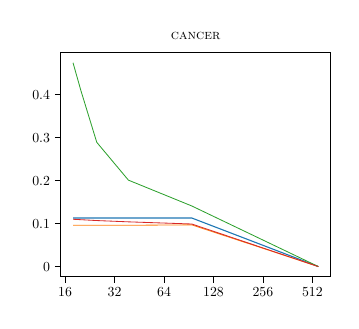
\begin{tikzpicture}[
scale=0.5
]

\definecolor{crimson2143940}{RGB}{214,39,40}
\definecolor{darkgray176}{RGB}{176,176,176}
\definecolor{darkorange25512714}{RGB}{255,127,14}
\definecolor{forestgreen4416044}{RGB}{44,160,44}
\definecolor{steelblue31119180}{RGB}{31,119,180}

\begin{axis}[
tick align=outside,
tick pos=left,
title={\sc cancer},
x grid style={darkgray176},
xmin=-8.8, xmax=536.8,
xtick style={color=black},
xtick={-100,0,100,200,300,400,500,600},
xticklabels={0,16,32,64,128,256,512,},
y grid style={darkgray176},
ymin=-0.0237, ymax=0.4977,
ytick style={color=black}
]
\addplot [thick, steelblue31119180]
table {%
16 0.113
32 0.113
64 0.113
128 0.113
256 0.113
512 0
};
\addplot [semithick, darkorange25512714]
table {%
16 0.096
32 0.096
64 0.096
128 0.096
256 0.097
512 0
};
\addplot [semithick, forestgreen4416044]
table {%
16 0.474
32 0.409
64 0.289
128 0.201
256 0.141
512 0
};
\addplot [semithick, crimson2143940]
table {%
16 0.11
32 0.109
64 0.107
128 0.104
256 0.099
512 0
};
\end{axis}

\end{tikzpicture}

%  \end{minipage}
%  \hfill
%  \begin{minipage}[t]{.16\textwidth}
%    \raggedleft
%    % This file was created with tikzplotlib v0.10.1.
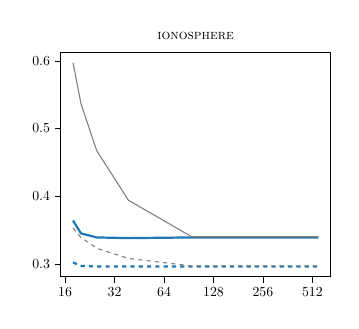
\begin{tikzpicture}[
scale=0.5
]

\definecolor{darkgray176}{RGB}{176,176,176}
\definecolor{gray}{RGB}{128,128,128}
\definecolor{steelblue31119180}{RGB}{31,119,180}

\begin{axis}[
tick align=outside,
tick pos=left,
title={\sc ionosphere},
x grid style={darkgray176},
xmin=-8.8, xmax=536.8,
xtick style={color=black},
xtick={-100,0,100,200,300,400,500,600},
xticklabels={0,16,32,64,128,256,512,},
y grid style={darkgray176},
ymin=0.28095, ymax=0.61205,
ytick style={color=black}
]
\addplot [ultra thick, steelblue31119180]
table {%
16 0.364
32 0.345
64 0.339
128 0.338
256 0.339
512 0.339
};
\addplot [ultra thick, steelblue31119180, dashed]
table {%
16 0.302
32 0.297
64 0.296
128 0.296
256 0.296
512 0.296
};
\addplot [thick, gray]
table {%
16 0.597
32 0.537
64 0.467
128 0.394
256 0.34
512 0.34
};
\addplot [thick, gray, dashed]
table {%
16 0.353
32 0.339
64 0.323
128 0.308
256 0.297
512 0.297
};
\end{axis}

\end{tikzpicture}

%  \end{minipage}
%  \hfill
  \begin{minipage}[t]{.16\textwidth}
    \raggedleft
    % This file was created by tikzplotlib v0.9.8.
\begin{tikzpicture}[scale=0.5]

\definecolor{color0}{rgb}{0.274509803921569,0.509803921568627,0.705882352941177}
\definecolor{color1}{rgb}{1,0.549019607843137,0}

\begin{axis}[
height=\figureheight,
tick align=outside,
tick pos=left,
title={\sc{Glass}},
width=\figurewidth,
x grid style={white!69.0196078431373!black},
xmin=-5, xmax=105,
xtick style={color=black},
xtick={-20,0,20,40,60,80,100,120},
xticklabels={\ensuremath{-}20,0,20,40,60,80,100,120},
y grid style={white!69.0196078431373!black},
ymin=0.645730930143993, ymax=1.81802513016566,
ytick style={color=black}
]
\path [draw=color0, fill=color0, opacity=0.1]
(axis cs:1,1.49771547138196)
--(axis cs:1,1.18952652316133)
--(axis cs:1,1.18266373930492)
--(axis cs:5,0.96605549198983)
--(axis cs:9,0.857698870422498)
--(axis cs:15,0.78946981593607)
--(axis cs:19,0.809266568098092)
--(axis cs:39,0.762809039558936)
--(axis cs:59,0.699017030144978)
--(axis cs:79,0.729237532733376)
--(axis cs:99,0.720662924824656)
--(axis cs:99,1.04896167752313)
--(axis cs:99,1.04896167752313)
--(axis cs:79,0.995374423453727)
--(axis cs:59,1.0311643117542)
--(axis cs:39,1.02993831156299)
--(axis cs:19,1.03639284358281)
--(axis cs:15,1.04105346761967)
--(axis cs:9,1.02568275842161)
--(axis cs:5,1.16679810278829)
--(axis cs:1,1.35410828283228)
--(axis cs:1,1.49771547138196)
--cycle;

\path [draw=color1, fill=color1, opacity=0.1]
(axis cs:1,1.76473903016467)
--(axis cs:1,1.58753965664686)
--(axis cs:1,1.57139842233233)
--(axis cs:5,1.35246612424739)
--(axis cs:9,1.24713571688454)
--(axis cs:15,1.14321333399575)
--(axis cs:19,1.11838605334277)
--(axis cs:39,0.956363946082652)
--(axis cs:59,0.843593507041992)
--(axis cs:79,0.782856534900766)
--(axis cs:99,0.743711704977892)
--(axis cs:99,1.01490281645003)
--(axis cs:99,1.01490281645003)
--(axis cs:79,1.04688512529527)
--(axis cs:59,1.08499783743299)
--(axis cs:39,1.12512608223656)
--(axis cs:19,1.27061408651308)
--(axis cs:15,1.26826043220348)
--(axis cs:9,1.56711712146726)
--(axis cs:5,1.55216843320769)
--(axis cs:1,1.6887418957198)
--(axis cs:1,1.76473903016467)
--cycle;

\addplot [semithick, color0]
table {%
1 1.34362099727164
1 1.2683860110686
5 1.06642679738906
9 0.941690814422055
15 0.915261641777871
19 0.922829705840453
39 0.896373675560965
59 0.865090670949587
79 0.862305978093552
99 0.884812301173894
};
\addplot [semithick, color1]
table {%
1 1.67613934340577
1 1.63007015902607
5 1.45231727872754
9 1.4071264191759
15 1.20573688309961
19 1.19450006992792
39 1.0407450141596
59 0.96429567223749
79 0.914870830098019
99 0.879307260713959
};
\end{axis}

\end{tikzpicture}

  \end{minipage}
  \hfill
  \begin{minipage}[t]{.16\textwidth}
    \raggedleft
    % This file was created with tikzplotlib v0.10.1.
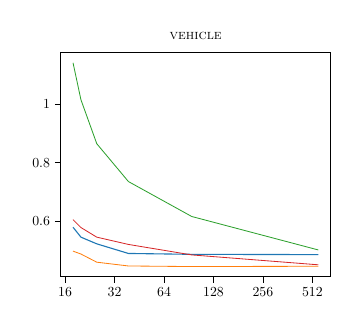
\begin{tikzpicture}[
scale=0.5
]

\definecolor{crimson2143940}{RGB}{214,39,40}
\definecolor{darkgray176}{RGB}{176,176,176}
\definecolor{darkorange25512714}{RGB}{255,127,14}
\definecolor{forestgreen4416044}{RGB}{44,160,44}
\definecolor{steelblue31119180}{RGB}{31,119,180}

\begin{axis}[
tick align=outside,
tick pos=left,
title={\sc vehicle},
x grid style={darkgray176},
xmin=-8.8, xmax=536.8,
xtick style={color=black},
xtick={-100,0,100,200,300,400,500,600},
xticklabels={0,16,32,64,128,256,512,},
y grid style={darkgray176},
ymin=0.408, ymax=1.178,
ytick style={color=black}
]
\addplot [thick, steelblue31119180]
table {%
16 0.578
32 0.544
64 0.521
128 0.488
256 0.485
512 0.484
};
\addplot [semithick, darkorange25512714]
table {%
16 0.496
32 0.486
64 0.458
128 0.445
256 0.443
512 0.444
};
\addplot [semithick, forestgreen4416044]
table {%
16 1.143
32 1.016
64 0.865
128 0.735
256 0.615
512 0.5
};
\addplot [semithick, crimson2143940]
table {%
16 0.604
32 0.577
64 0.544
128 0.519
256 0.483
512 0.449
};
\end{axis}

\end{tikzpicture}

  \end{minipage}
  \hfill
  \begin{minipage}[t]{.16\textwidth}
    \raggedleft
    % This file was created with tikzplotlib v0.10.1.
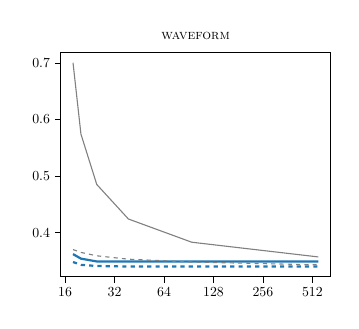
\begin{tikzpicture}[
scale=0.5
]

\definecolor{darkgray176}{RGB}{176,176,176}
\definecolor{gray}{RGB}{128,128,128}
\definecolor{steelblue31119180}{RGB}{31,119,180}

\begin{axis}[
tick align=outside,
tick pos=left,
title={\sc waveform},
x grid style={darkgray176},
xmin=-8.8, xmax=536.8,
xtick style={color=black},
xtick={-100,0,100,200,300,400,500,600},
xticklabels={0,16,32,64,128,256,512,},
y grid style={darkgray176},
ymin=0.322, ymax=0.718,
ytick style={color=black}
]
\addplot [ultra thick, steelblue31119180]
table {%
16 0.362
32 0.354
64 0.349
128 0.349
256 0.349
512 0.349
};
\addplot [ultra thick, steelblue31119180, dashed]
table {%
16 0.348
32 0.343
64 0.341
128 0.34
256 0.34
512 0.34
};
\addplot [thick, gray]
table {%
16 0.7
32 0.574
64 0.485
128 0.424
256 0.383
512 0.357
};
\addplot [thick, gray, dashed]
table {%
16 0.37
32 0.365
64 0.359
128 0.353
256 0.348
512 0.343
};
\end{axis}

\end{tikzpicture}

  \end{minipage}
  \hfill
  \begin{minipage}[t]{.16\textwidth}
    \raggedleft
    % This file was created with tikzplotlib v0.10.1.
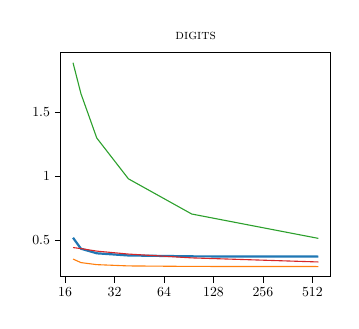
\begin{tikzpicture}[
scale=0.5
]

\definecolor{crimson2143940}{RGB}{214,39,40}
\definecolor{darkgray176}{RGB}{176,176,176}
\definecolor{darkorange25512714}{RGB}{255,127,14}
\definecolor{forestgreen4416044}{RGB}{44,160,44}
\definecolor{steelblue31119180}{RGB}{31,119,180}

\begin{axis}[
tick align=outside,
tick pos=left,
title={\sc digits},
x grid style={darkgray176},
xmin=-8.8, xmax=536.8,
xtick style={color=black},
xtick={-100,0,100,200,300,400,500,600},
xticklabels={0,16,32,64,128,256,512,},
y grid style={darkgray176},
ymin=0.2101, ymax=1.9679,
ytick style={color=black}
]
\addplot [ultra thick, steelblue31119180]
table {%
16 0.516
32 0.43
64 0.394
128 0.377
256 0.37
512 0.368
};
\addplot [thick, darkorange25512714]
table {%
16 0.349
32 0.321
64 0.305
128 0.295
256 0.291
512 0.29
};
\addplot [thick, forestgreen4416044]
table {%
16 1.888
32 1.646
64 1.298
128 0.978
256 0.702
512 0.511
};
\addplot [thick, crimson2143940]
table {%
16 0.439
32 0.431
64 0.411
128 0.388
256 0.358
512 0.326
};
\end{axis}

\end{tikzpicture}

  \end{minipage}
  \hfill
  \begin{minipage}[t]{.16\textwidth}
    \raggedleft
    % This file was created with tikzplotlib v0.10.1.
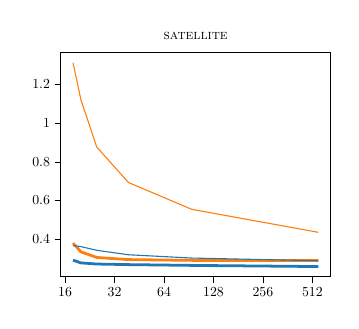
\begin{tikzpicture}[
scale=0.5
]

\definecolor{darkgray176}{RGB}{176,176,176}
\definecolor{darkorange25512714}{RGB}{255,127,14}
\definecolor{steelblue31119180}{RGB}{31,119,180}

\begin{axis}[
tick align=outside,
tick pos=left,
title={\sc satellite},
x grid style={darkgray176},
xmin=-8.8, xmax=536.8,
xtick style={color=black},
xtick={-100,0,100,200,300,400,500,600},
xticklabels={0,16,32,64,128,256,512,},
y grid style={darkgray176},
ymin=0.2053, ymax=1.3647,
ytick style={color=black}
]
\addplot [line width=2pt, darkorange25512714]
table {%
16 0.379
32 0.334
64 0.305
128 0.294
256 0.29
512 0.289
};
\addplot [line width=2pt, steelblue31119180]
table {%
16 0.291
32 0.277
64 0.271
128 0.268
256 0.264
512 0.258
};
\addplot [thick, darkorange25512714]
table {%
16 1.312
32 1.12
64 0.876
128 0.693
256 0.554
512 0.435
};
\addplot [thick, steelblue31119180]
table {%
16 0.367
32 0.361
64 0.342
128 0.319
256 0.302
512 0.288
};
\end{axis}

\end{tikzpicture}

  \end{minipage}\\[-1em]
  %
  % Legend  
  \definecolor{steelblue31119180}{RGB}{31,119,180}
  \definecolor{darkorange25512714}{RGB}{255,127,14}  
  \newcommand{\myline}[1]{\protect\tikz[baseline=-.5ex,line width=1.6pt]\protect\draw[draw=#1](0,0)--(1.2em,0);}
  \caption{Comparison of convergence in terms of number of inducing points $M$ in NLPD (mean over 10 seeds) on UCI classification tasks: \our (thick) vs.\ subsets (\cite{immer2021improving}, thin). Orange lines (\myline{darkorange25512714}) use the GP mean, whereas blue lines (\myline{steelblue31119180}) the NN MAP estimate as mean. Our \our converges fast for all cases.\looseness-1}
  \label{fig:uci}
  %\vspace*{-6pt}
\end{figure}



\subsection{Capturing uncertainty in UCI tasks under supervised learning}
\label{sec:uci}
%
We first evaluate \our on eight UCI benchmarks~\cite{UCI}, a variety of binary and multi-class classification tasks with different data set sizes.
We train a two-layer MLP for each of the classification tasks and follow the experiment set up in \cite{immer2021improving}.
%by using the same hyperparameters, performing a hyperparameter search over the prior precision $\delta$,
% We follow \cite{immer2021improving} by using the same hyperparameters, performing a hyperparameter search over the prior precision $\delta$,
% and run the experiment over $10$ random splits.
% That is, after training we construct the \our dual and use the resulting model for uncertainty quantification.
% for the neural network training as in the UCI experiments of
\cref{tbl:uci} (left) shows that \our with $M=256$ either matches or outperforms the predictive performance of the NN MAP, mean-field VI, Bayesian NN, and GLM
predictions %in terms of negative log-predictive density (NLPD).
(baselines from \cite{immer2021improving}).
That is, we match predictive performance despite being sparse.

In \cref{tbl:uci} (right) we compare to the subset GP method from \cite{immer2021improving} whilst using only $M=32$ inducing points.
It shows that \our is able to summarize the full data set more effectively than the GP subset method as it maintains predictive performance
whilst using fewer inducing points.
\cref{fig:uci} further shows that as the number of inducing points is lowered $M=512,\ldots, 16$, \our is able to maintain a much better NLPD than the GP subset.
These results demonstrate \our's sparse representation captures information from the entire data set and as a result provides good uncertainty estimates.
We provide full details of our experiments and further results using $M=16,32,64,128,256$ in \cref{app:uci}.
% benefits of \our in summarizing the full data distribution onto a small set of inducing
% points over just picking a random subset.



% We match the predictive performance despite being sparse (here, $M=256$).


% This is
% However, our method used

% despite being sparse (here, $M=256$).

% (left), we compare our model to the NN MAP estimate, mean-field VI, a Bayesian NN, and a GLM model (see \cite{immer2021improving} for the baselines) in negative log-predictive density (NLPD).
% In \cref{tbl:uci} (left), we compare our model to the NN MAP estimate, mean-field VI, a Bayesian NN, and a GLM model (see \cite{immer2021improving} for the baselines) in negative log-predictive density (NLPD).
% We match the predictive performance despite being sparse (here, $M=256$).
% Results for $M=16,32,64,128,256$ are included in \cref{app:uci} with full experiment details.

% \cref{tbl:uci} (right) shows that \our is able to summarize the information of the full data set more efficiently than the sparse GP subset method.
% As a result, it maintains predictive performance whilst using fewer inducing points.
% This is even more apparent from \cref{fig:uci} which shows the benefits of \our in summarizing the full data distribution onto a small set of inducing points over just picking a random subset.

% In \cref{tbl:uci} (right), we also include an ablation and comparison study (to \cite{immer2021improving}) with a fixed low number of inducing points ($M=32$).
% The comparison shows that our sparse method is able to summarize the information of the full data set more efficiently than sparse subset methods, and can match the performance of the full GP even with a low number of inducing points. This is even more apparent from \cref{fig:uci} which shows the benefits of \our in summarizing the full data distribution onto a small set of inducing points over just picking a random subset.



% see \cref{tbl:uci} for a list of the datasets. The neural network training was done using MAP, with a prior $\mathcal{N}(0,\delta^{-1} \MI)$ with prior precision $\delta$. After training, we constructed the SVGP dual and used the resulting SVGP model for uncertainty quantification. Depending on task dimension and complexity, our model can match the NN MAP in NLPD performance even with a low number of inducing points, see \cref{tbl:uci}. We performed hyperparameter search over the prior precision, and ran the experiment over $10$ seeds. During the initial NN training, we used a learning rate of $1e-3$.

%\begin{figure}
%  \raggedleft\scriptsize
%  \setlength{\figurewidth}{\textwidth}
%  \setlength{\figureheight}{.55\figurewidth}
%  %\pgfplotsset{axis on top,ymajorgrids,axis line style={draw=none},legend style={at={(-.1,-.1)},anchor=north east}}
%  %\pgfplotsset{grid style={line width=.1pt, draw=gray!10,dashed}}
%  %\def\our{{\sc sfr} (ours)}
%  % This file was created with tikzplotlib v0.10.1.
\begin{tikzpicture}

\definecolor{crimson2143940}{RGB}{214,39,40}
\definecolor{darkgray176}{RGB}{176,176,176}
\definecolor{darkorange25512714}{RGB}{255,127,14}
\definecolor{darkturquoise23190207}{RGB}{23,190,207}
\definecolor{forestgreen4416044}{RGB}{44,160,44}
\definecolor{goldenrod18818934}{RGB}{188,189,34}
\definecolor{gray127}{RGB}{127,127,127}
\definecolor{lightgray204}{RGB}{204,204,204}
\definecolor{mediumpurple148103189}{RGB}{148,103,189}
\definecolor{orchid227119194}{RGB}{227,119,194}
\definecolor{sienna1408675}{RGB}{140,86,75}
\definecolor{steelblue31119180}{RGB}{31,119,180}

\begin{axis}[
height=\figureheight,
legend cell align={left},
legend style={fill opacity=0.8, draw opacity=1, text opacity=1, draw=lightgray204},
tick align=outside,
tick pos=left,
width=\figurewidth,
x grid style={darkgray176},
xmin=-0.2, xmax=4.2,
xtick style={color=black},
xtick={0,1,2,3,4},
xtick={0,1,2,3,4},
xtick={0,1,2,3,4},
xtick={0,1,2,3,4},
xtick={0,1,2,3,4},
xtick={0,1,2,3,4},
xtick={0,1,2,3,4},
xtick={0,1,2,3,4},
xtick={0,1,2,3,4},
xtick={0,1,2,3,4},
xtick={0,1,2,3,4},
xtick={0,1,2,3,4},
xtick={0,1,2,3,4},
xtick={0,1,2,3,4},
xtick={0,1,2,3,4},
xticklabels={256,512,1024,2048,3200},
xticklabels={256,512,1024,2048,3200},
xticklabels={256,512,1024,2048,3200},
xticklabels={256,512,1024,2048,3200},
xticklabels={256,512,1024,2048,3200},
xticklabels={256,512,1024,2048,3200},
xticklabels={256,512,1024,2048,3200},
xticklabels={256,512,1024,2048,3200},
xticklabels={256,512,1024,2048,3200},
xticklabels={256,512,1024,2048,3200},
xticklabels={256,512,1024,2048,3200},
xticklabels={256,512,1024,2048,3200},
xticklabels={256,512,1024,2048,3200},
xticklabels={256,512,1024,2048,3200},
xticklabels={256,512,1024,2048,3200},
y grid style={darkgray176},
ymin=-0.567324956290268, ymax=13.0270240820956,
ytick style={color=black}
]
\addplot [semithick, steelblue31119180]
table {%
0 2.450651686371
1 2.33688367659858
2 0.758006683252107
3 0.418063571567222
4 0.293906180967752
};
\addlegendentry{\sc GP subset}
\addplot [semithick, darkorange25512714]
table {%
0 1.12153317466841
1 0.85325292908048
2 12.4090991258054
3 0.0672844892936739
4 0.0627872786062761
};
\addlegendentry{\sc \our}
\addplot [semithick, forestgreen4416044]
table {%
0 1.30682946689449
1 1.27447684300892
2 0.0822643172822197
3 0.0732855173563596
4 0.0692346420741961
};
\addlegendentry{\sc GP subset (NN)}
\addplot [semithick, crimson2143940]
table {%
0 0.732772882751394
1 0.638123397907866
2 12.3951401856728
3 0.0738436001185355
4 0.0710273410515106
};
\addlegendentry{\sc \our (NN)}
\addplot [semithick, mediumpurple148103189, dashed]
table {%
0 1.6746972458165
1 1.6746972458165
2 1.6746972458165
3 1.6746972458165
4 1.6746972458165
};
\addlegendentry{\sc bnn}
\addplot [semithick, sienna1408675, dashed]
table {%
0 0.921512236735063
1 0.921512236735063
2 0.921512236735063
3 0.921512236735063
4 0.921512236735063
};
\addlegendentry{\sc glm}
\addplot [semithick, orchid227119194, dashed]
table {%
0 0.0677361758804467
1 0.0677361758804467
2 0.0677361758804467
3 0.0677361758804467
4 0.0677361758804467
};
\addlegendentry{\sc map}
\addplot [semithick, gray127]
table {%
0 0.0982
1 0.1364
2 0.7276
3 0.8718
4 0.9124
};
\addlegendentry{\sc GP subset}
\addplot [semithick, goldenrod18818934]
table {%
0 0.921
1 0.9598
2 0.0532
3 0.981
4 0.98
};
\addlegendentry{\sc \our}
\addplot [semithick, darkturquoise23190207]
table {%
0 0.9012
1 0.9088
2 0.9764
3 0.9764
4 0.9786
};
\addlegendentry{\sc GP subset (NN)}
\addplot [semithick, steelblue31119180]
table {%
0 0.971
1 0.97
2 0.0506
3 0.9778
4 0.9774
};
\addlegendentry{\sc \our (NN)}
\addplot [semithick, darkorange25512714, dashed]
table {%
0 0.7622
1 0.7622
2 0.7622
3 0.7622
4 0.7622
};
\addlegendentry{\sc bnn}
\addplot [semithick, forestgreen4416044, dashed]
table {%
0 0.9254
1 0.9254
2 0.9254
3 0.9254
4 0.9254
};
\addlegendentry{\sc glm}
\addplot [semithick, crimson2143940, dashed]
table {%
0 0.9788
1 0.9788
2 0.9788
3 0.9788
4 0.9788
};
\addlegendentry{\sc map}
\end{axis}

\end{tikzpicture}

%  \caption{Foo}
%  \label{fig:mnist}
%\end{figure}
%





\subsection{Supervised learning on image data sets}
\label{sec:image}

\begin{table}[t!] 
  \centering\scriptsize
  \caption{Metrics for supervised learning on image data with a CNN. We report accuracy, NLPD, and expected calibration error (mean$\pm$std) over 10 seeds. Our \our method is able to match the full methods using only a sparse set. For the GP predictive sparse subset method and \our we report results both using the NN MAP as mean (NN) and using the GP mean.} 
	\label{tbl:imagesuper}
	% Control table spacing
	\renewcommand{\arraystretch}{1.}
	\setlength{\tabcolsep}{6pt}
	\setlength{\tblw}{0.095\textwidth}  
	
	% Custom error formatting
	\newcommand{\val}[2]{%
		$#1$\textcolor{gray}{\tiny ${\pm}#2$}
	} 

    % THE TABLE CAN BE FORMATTED MORE LIKE THIS
    % \begin{tabular}{l l C{\tblw} C{\tblw} C{\tblw} C{\tblw}}
    % \toprule
    % & Method & ACC~$\uparrow$ & NLPD~$\downarrow$ & ECE~$\downarrow$ & OOD-AUC~$\uparrow$  \\
    % \midrule
    % \multirow{2}{*}{FMNIST}
    % & MAP & \val{0.000}{0.000} & \val{0.000}{0.000} & \val{0.000}{0.000} & \val{0.000}{0.000} \\
    % & BNN predictive & \val{0.000}{0.000} & \val{0.000}{0.000} & \val{0.000}{0.000} & \val{0.000}{0.000} \\
    % & BNN predictive \cite{todo} & \val{0.000}{0.000} & \val{0.000}{0.000} & \val{0.000}{0.000} & \val{0.000}{0.000} \\
    % & GLM predictive & \val{0.000}{0.000} & \val{0.000}{0.000} & \val{0.000}{0.000} & \val{0.000}{0.000} \\
    % & GP predictive & \val{0.000}{0.000} & \val{0.000}{0.000} & \val{0.000}{0.000} & \val{0.000}{0.000} \\
    % & \our (NN) & \val{0.000}{0.000} & \val{0.000}{0.000} & \val{0.000}{0.000} & \val{0.000}{0.000} \\
    % & \our & \val{0.000}{0.000} & \val{0.000}{0.000} & \val{0.000}{0.000} & \val{0.000}{0.000} \\
    % \midrule
    % \multirow{2}{*}{CIFAR-10}
    % & MAP & \val{0.000}{0.000} & \val{0.000}{0.000} & \val{0.000}{0.000} & \val{0.000}{0.000} \\
    % & BNN predictive & \val{0.000}{0.000} & \val{0.000}{0.000} & \val{0.000}{0.000} & \val{0.000}{0.000} \\
    % & BNN predictive \cite{todo} & \val{0.000}{0.000} & \val{0.000}{0.000} & \val{0.000}{0.000} & \val{0.000}{0.000} \\
    % & GLM predictive & \val{0.000}{0.000} & \val{0.000}{0.000} & \val{0.000}{0.000} & \val{0.000}{0.000} \\
    % & GP predictive & \val{0.000}{0.000} & \val{0.000}{0.000} & \val{0.000}{0.000} & \val{0.000}{0.000} \\
    % & \our (NN) & \val{0.000}{0.000} & \val{0.000}{0.000} & \val{0.000}{0.000} & \val{0.000}{0.000} \\
    % & \our & \val{0.000}{0.000} & \val{0.000}{0.000} & \val{0.000}{0.000} & \val{0.000}{0.000} \\
    % \bottomrule
    % \end{tabular}
  \newcommand{\myline}{\protect\tikz[baseline=-.5ex,line width=.7pt]\protect\draw[draw=gray](0,0)--(7em,0);}
  \begin{tabular}{l c C{\tblw} C{\tblw} C{\tblw} C{\tblw} C{\tblw} C{\tblw}}
    \toprule
            &     &  \multicolumn{3}{c}{\myline~MNIST~\myline} & \multicolumn{3}{c}{\myline~FMNIST~\myline} \\
     Method & $M$ & ACC~$\uparrow$ & NLPD~$\downarrow$ & ECE~$\downarrow$ & ACC~$\uparrow$ & NLPD~$\downarrow$ & ECE~$\downarrow$ \\
    \midrule
    %\multirow{2}{*}{MNIST}
    MAP & -- & \val{98.22}{0.13} & \val{0.061}{0.004} & \val{0.006}{0.001}
          & \val{91.39}{0.11} & \val{0.258}{0.004} & \val{0.017}{0.001} \\
    BNN predictive \cite{immer2021improving} & -- & \val{93.14}{0.05} & \val{0.304}{0.002} & \val{0.111}{0.003}
                                               & \val{84.42}{0.12} & \val{0.942}{0.016} & \val{0.411}{0.008} \\
    BNN predictive \cite{ritter2018kfac} & -- & \val{93.03}{0.13} & \val{0.369}{0.003} & \val{0.168}{0.001}
                                           & \val{91.20}{0.07} & \val{0.265}{0.004} & \val{0.024}{0.002} \\
    GLM predictive \cite{immer2021improving} & -- & \val{98.40}{0.05} & \val{0.054}{0.002} & \val{0.007}{0.001}
                                               & \val{92.25}{0.10} & \val{0.244}{0.003} & \val{0.012}{0.003} \\\arrayrulecolor{black!10}\midrule 
    GP predictive \cite{immer2021improving} & $3200$ & \val{\textbf{98.22}}{0.13} & \val{\textbf{0.058}}{0.001} & \val{\textbf{0.003}}{0.000}
                                                     & \val{91.36}{0.11} & \val{\textbf{0.25}}{0.004} & \val{\textbf{0.007}}{0.001} \\

    GP predictive (NN) & $1024$ & \val{97.70}{0.07} & \val{0.080}{0.002} & \val{0.011}{0.001}
                              & \val{\textbf{91.47}}{0.41} & \val{0.289}{0.009} & \val{0.033}{0.003} \\

    GP predictive & $1024$  & \val{76.28}{1.85} & \val{0.702}{0.029} & \val{0.070}{0.022}
                            & \val{83.98}{0.35} & \val{0.503}{0.012} & \val{0.052}{0.006} \\
    \our (NN) & $1024$ &  \val{98.02}{0.12} & \val{0.066}{0.003} & \val{0.007}{0.001}
                     & \val{\textbf{91.93}}{0.45} & \val{0.267}{0.011} & \val{0.028}{0.003} \\
    \our & $1024$ & \val{\textbf{98.07}}{0.06} & \val{0.063}{0.003} & \val{0.005}{0.001}
                  & \val{\textbf{91.56}}{0.35} & \val{\textbf{0.253}}{0.006} & \val{0.012}{0.001} \\
%    \multirow{2}{*}{FMNIST}
%    & MAP & \val{91.39}{0.11} & \val{0.258}{0.004} & \val{0.017}{0.001} \\
    %& BNN predictive \cite{immer2021improving} & \val{84.42}{0.12} & \val{0.942}{0.016} & \val{0.411}{0.008} \\
    % & BNN predictive \cite{ritter2018kfac} & \val{91.20}{0.07} & \val{0.265}{0.004} & \val{0.024}{0.002} \\
    % & GLM predictive \cite{immer2021improving} & \val{92.25}{0.10} & \val{0.244}{0.003} & \val{0.012}{0.003} \\
    %& GP predictive \cite{immer2021improving} $m=3200$ & \val{91.36}{0.11} & \val{0.25}{0.004} & \val{0.007}{0.001} \\
    % & GP predictive NN $m=1024$ &  \val{0}{0.07} & \val{0}{0.002} & \val{0}{0.001} \\
    % & GP predictive $m=1024$  &  \val{0}{1.85} & \val{0}{0.029} & \val{0}{0.022} \\
    % & \our NN $m=1024$ &  \val{0}{0.0} & \val{0}{0.003} & \val{0}{0.001} \\
    % & \our $m=1024$ &  \val{0}{0.06} & \val{0}{0.003} & \val{0}{0.001} \\
    \arrayrulecolor{black}
    \bottomrule
  \end{tabular}

% & \sc \sc gp predictive  &  \val{76.28333}{1.849} & \val{0.70168}{0.02883} & \val{0.07049}{0.02154} \\
% & \sc \sc gp predictive NN \cite{immer2021improving} &  \val{97.70333}{0.074} & \val{0.08027}{0.00248} & \val{0.01052}{0.00097} \\
% & \sc \our &  \val{98.06667}{0.060} & \val{0.06312}{0.00284} & \val{0.00493}{0.00086} \\
% & \sc \our NN &  \val{98.02000}{0.122} & \val{0.06583}{0.00294} & \val{0.00714}{0.00096} \\
% M=512
% & \sc \our &  \val{96.05}{0.00} & \val{0.85}{0.01} & \val{0.50}{0.00} \\
% & \sc \sc gp predictive  &  \val{14.79}{0.01} & \val{2.30}{0.02} & \val{0.02}{0.01} \\
% & \sc \sc gp predictive NN \cite{immer2021improving} &  \val{91.49}{0.01} & \val{1.25}{0.01} & \val{0.61}{0.00} \\
% & \sc \our NN &  \val{96.96}{0.00} & \val{0.63}{0.00} & \val{0.40}{0.00} \\

% M=1024

    % THE TABLE NUMBER ARE GENERATED BY A SCRIPT	
	%\begin{tabular}{l C{0.6\tblw} C{0.6\tblw} C{0.6\tblw} C{0.6\tblw} C{0.6\tblw}  C{0.6\tblw}}
\toprule
& acc & nll & ece & ood-auc  \\
\midrule
\sc FMNIST and MAP & \val{91.39}{0.11} & \val{0.258}{0.004} & \val{0.017}{0.001} & \val{0.864}{0.014} \\
\sc FMNIST and BNN predictive & \val{84.42}{0.12} & \val{0.942}{0.016} & \val{0.411}{0.008} & \val{0.945}{0.002} \\
\sc FMNIST and BNN predictive (Ritter et al.) & \val{91.2}{0.07} & \val{0.265}{0.004} & \val{0.024}{0.002} & \val{0.947}{0.006} \\
\sc FMNIST and GLM predictive & \val{92.25}{0.1} & \val{0.244}{0.003} & \val{0.012}{0.003} & \val{0.955}{0.006} \\
\sc FMNIST and GP predictive & \val{91.36}{0.11} & \val{0.25}{0.004} & \val{0.007}{0.001} & \val{0.918}{0.01} \\
\sc FMNIST and SVGP (100) & \val{88.188}{0.756} & \val{0.357}{0.017} & \val{0.063}{0.006} & \val{0.0}{0.0} \\
\sc FMNIST and SVGP NN (100) & \val{90.052}{0.371} & \val{0.3}{0.01} & \val{0.054}{0.004} & \val{0.0}{0.0} \\
\sc FMNIST and SVGP (500) & \val{90.224}{0.656} & \val{0.292}{0.01} & \val{0.048}{0.002} & \val{0.0}{0.0} \\
\sc FMNIST and SVGP NN (500) & \val{90.376}{0.55} & \val{0.281}{0.009} & \val{0.038}{0.003} & \val{0.0}{0.0} \\
\sc FMNIST and SVGP (1000) & \val{90.892}{0.443} & \val{0.265}{0.008} & \val{0.009}{0.003} & \val{0.0}{0.0} \\
\sc FMNIST and SVGP NN (1000) & \val{90.788}{0.435} & \val{0.265}{0.009} & \val{0.013}{0.003} & \val{0.0}{0.0} \\
\sc CIFAR10 and MAP & \val{80.92}{0.32} & \val{0.605}{0.007} & \val{0.066}{0.004} & \val{0.792}{0.008} \\
\sc CIFAR10 and BNN predictive & \val{21.74}{0.8} & \val{2.114}{0.021} & \val{0.095}{0.012} & \val{0.689}{0.02} \\
\sc CIFAR10 and BNN predictive (Ritter et al.) & \val{80.78}{0.36} & \val{0.588}{0.005} & \val{0.052}{0.005} & \val{0.783}{0.007} \\
\sc CIFAR10 and GLM predictive & \val{81.37}{0.15} & \val{0.601}{0.008} & \val{0.084}{0.01} & \val{0.843}{0.016} \\
\sc CIFAR10 and GP predictive & \val{81.01}{0.32} & \val{0.555}{0.008} & \val{0.017}{0.003} & \val{0.82}{0.013} \\
\sc CIFAR10 and SVGP (100) & \val{70.68}{0.684} & \val{0.952}{0.018} & \val{0.172}{0.005} & \val{0.0}{0.0} \\
\sc CIFAR10 and SVGP NN (100) & \val{75.672}{0.812} & \val{0.767}{0.016} & \val{0.121}{0.01} & \val{0.0}{0.0} \\
\sc CIFAR10 and SVGP (500) & \val{75.272}{0.724} & \val{0.768}{0.015} & \val{0.107}{0.009} & \val{0.0}{0.0} \\
\sc CIFAR10 and SVGP NN (500) & \val{75.788}{0.731} & \val{0.738}{0.017} & \val{0.089}{0.009} & \val{0.0}{0.0} \\
\sc CIFAR10 and SVGP (1000) & \val{76.516}{0.639} & \val{0.76}{0.029} & \val{0.064}{0.007} & \val{0.0}{0.0} \\
\sc CIFAR10 and SVGP NN (1000) & \val{76.124}{0.894} & \val{0.893}{0.045} & \val{0.117}{0.009} & \val{0.0}{0.0} \\
\bottomrule
\end{tabular}

\end{table}

Similarly to the UCI experiments, we seek to demonstrate \our on image data that features more complicated data manifolds and model structures.
We consider the MNIST and Fashion-MNIST (FMNIST) classification tasks, and use an MLP and a CNN architecture respectively (matching the setup in \cite{immer2021improving}).
After training, we computed the duals for \our and use the model for prediction (full experiment details in \cref{app:image}).
In \cref{tbl:imagesuper}, we compare to baselines also used in \cite{immer2021improving}.
We report accuracy (ACC), NLPD, and expected calibration error (ECE).
For \our and the GP predictive subset method by \cite{immer2021improving}, we provide results when predicting with GP mean and when using the neural network (NN) and
fix the number of inducing points $M=1024$.
For completeness, we also include the GP predictive result from \cite{immer2021improving} which used more inducing points $M=3200$.
The results in \cref{tbl:imagesuper} agree with the conclusions drawn from the UCI experiments showing that \our is able to more efficiently capture the posterior using a sparse set of points.
They further demonstrate that \our's predictive mean (GP) significantly outperforms the GP predictive subset.
This is an interesting result as we cannot rely on the NN's prediction if we wish to condition on new data, using the dual conditioning from \label{sec:sequential}.
In this setting, we must rely on our GP's predictive mean.
% Other approaches, \cite{immer2021improving} never inten
% The resutls demonstrate that \our's predictive GP mean significantly outperforms the
These results on image data sets motivate experiments beyond the supervised learning setting, which we now detail.

% For \our and the GP predictive subset method by \cite{immer2021improving} we fix the number of points $M=1024$.



%We performed hyperparameter optimization over the prior precision, and found the optimal value to be [insert]. We ran the experiment over $5$ seeds. During the NN training, we used a batch size of $512$ and an Adam optimizer with learning rate $1e-3$.

%In addition to uncertainty estimates, our method can update the posterior when given new data. We gave the SVGP model 10 \% of the test dataset used for evaluation, and compare the performance of the SVGP model and the retrained NN in [INSERT TABLE]. 



\subsection{Updating the network representation in continual learning}
\label{sec:cl-exp}
%
%%% Very rough draft
%This experiment's section is meant to demonstrate the quality of our sparse representation to retain previous knowledge in the Continual learning setting. Unfortunately the CL literature is based on methods that require very diverse set of hyperparameters 
%% Idea: it is very difficult to have everything under control, because model changes, settings change, optimizer change, and so on. Then what we did was trying to replicate as close as possible the results for the competing methods by using their codebases where available and choosing the hyperpameters accordingly to their choices.
%
%% Why SH?
%% TODO: there are at least two papers that clearly say MH is unrealistic and too simple as a consequence is not a good way to assess the quality of the method
%
%% Architectures
%We conduct the experiments on a set of three CL benchmarks Sequential-MNIST (S-MNIST), Sequential-FashionMNIST (S-FMNIST), and Permuted-MNIST (P-MNIST).  Following \cite{rudner2022continual, pan2020continual}, we used a two-layer MLP with 256 hidden units with ReLU activation for S-MNIST and S-FMNIST, and a two-layer with 100 hidden units for P-MNIST. 
%
%% Methods
%We compared our method to 1) weight-regularization based methods EWC, SI and VCL (which also has the addition of coresets); 2) function-based regularization based methods DER, FROMP, S-FSVI, SFR; 3) an ablation for which we replace $\bar{\MB}^{-1}$ with an identity matrix $\MI_m$, \ie which is equivalent to assuming a GP with iid realization \todo{Not sure this is 100$\%$ correct}.
%% Inducing points
%Following \citep{rudner2022continual}, we use 200 inducing points per tasks % this one can be difficult to justify since S-FSVI samples 200 context points and then iteratively samples 40 coresets points (or at least that's what I got)
%on all the inducing points, and a lower number of inducing point for S-MNIST, to investigate if our method was still capable of capture more information due to its sparse formulation, as explained in \cref{todo}.
%
%%% Questions: Should we also mention the Identity outside when not trained on those classes or just leave that for the appendix?



\setlength{\columnsep}{8pt}
\setlength{\intextsep}{0pt}
\begin{wraptable}{R}{.65\textwidth}
  \centering\scriptsize
  \caption{Continual learning experiments. We report accuracy${\pm}$std and bold based on a $t$-test. $^*$Methods rely on weight regularization.}
  %\textcolor{blue}{Results from \cite{rudner2022continual}
  %\color{red}{Preliminary results need more runs or hyperparam tuning}
	\label{tbl:cl_table_1}
	
	% Control table spacing
	\renewcommand{\arraystretch}{1.}
	\setlength{\tabcolsep}{1pt}
	\setlength{\tblw}{0.14\textwidth}  
	
	% Custom error formatting
	\newcommand{\val}[2]{%
		$#1$\textcolor{gray}{\tiny ${\pm}#2$}
	} 
	
	\vspace*{-4pt}
	
	% Import table content
	\begin{tabular}{@{}lcccc@{}}
\toprule
 Method           & 
\begin{tabular}[c]{c}S-MNIST (SH) \\ 200 points\end{tabular} & 
\begin{tabular}[c]{c}S-MNIST (SH) \\ 1000 points\end{tabular} & 
\begin{tabular}[c]{c}S-FMNIST (SH)\\ 1000 points\end{tabular} & 
\begin{tabular}[c]{c}P-MNIST (SH) \\ 1000 points\end{tabular} \\ \midrule
%% Weight Regularization Methods
{\sc Online-EWC}~\cite{schwarz2018progress}$^*$ & \val{19.95}{0.28} & \val{19.95}{0.28} & \val{19.48}{0.01} & \val{74.87}{1.81}\\
{\sc SI}~\cite{zenke2017continual}$^*$ & \val{19.82}{0.09} & \val{19.82}{0.09} & \val{19.80}{0.21} & \val{88.39}{1.37}\\
{\sc VCL} (with coresets)~\cite{nguyen2018variational} & \val{22.31}{2.00} & \val{32.11}{1.16}\color{blue}{*} & \val{53.59}{3.74} &  \val{92.84}{0.34}\\
%{\sc VCL} (no coreset) & \val{}{} & \color{blue}{\val{17.74}{1.20}} & \val{}{} & \color{blue}{\val{87.50}{0.61}}\\
\midrule
%% Functional Regularization Methods
{\sc DER}~\cite{buzzega2020dark} & \val{85.26}{0.54} & \val{92.13}{0.45} & \val{\bf 82.03}{0.57} & \val{91.53}{0.26} \\
{\sc FROMP}~\cite{pan2020continual} & \val{75.21}{2.05} & \val{89.54}{0.72} & \val{78.83}{0.46} & \val{94.90}{0.04}\color{blue}{*}\\
{\sc S-FSVI}~\cite{rudner2022continual} & \val{84.51}{1.30} & \val{92.87}{0.14}\color{blue}{*} & \val{77.54}{0.40} & \val{\bf 95.76}{0.02}\color{blue}{*} \\
{\sc SFR}~(Ours) & \val{88.73}{0.31} & \val{94.19}{0.26} & \val{\bf 81.96}{0.24} & \val{94.95}{0.14}\\
%{\sc L2} & \val{87.48}{0.81} & \val{93.98}{0.17} & \val{81.20}{0.30} & \val{93.89}{0.07}\\
 \hspace{2mm} {\sc L2} (Ours) abl. & \val{88.14}{0.86} & \val{\bf 93.72}{0.10} & \val{81.21}{0.36} & \val{94.54}{0.11}\\
\bottomrule
\end{tabular}

\end{wraptable}
%
% Overview
We show how the regularizer described in \cref{sec:sequential} can be used in continual learning to retain a compact representation of the neural network.
The experiments are run only in the single-head (SH) setting that is harder and more realistic than multi-head (MH) (see discussion in \citep{van2019three}).	
% Benchmarks/architectures
 Our regularizer is evaluated on three CL benchmarks, specifically Split-MNIST (S-MNIST), Split-FashionMNIST (S-FMNIST), and the 10-tasks Permuted-MNIST (P-MNIST). We adhere to the same setups outlined in \cite{rudner2022continual, pan2020continual}, which use a two-layer MLP with 256 hidden units and ReLU activation for S-MNIST and S-FMNIST and a two-layer MLP with 100 hidden units for P-MNIST, to ensure consistency (see \cref{app:cl-exp} for full details).

% Methods
We compare our method against two categories of methods: {\em (i)}~weight-regularization methods: EWC, SI, and VCL (with coresets), and {\em(ii)}~function-based regularization methods: DER, FROMP, and S-FSVI. We also introduce an ablation study where we replace $\bar{\MB}_t^{-1}$ with an identity matrix $\MI_M$, equivalent to using an L2 regularizer on the function outputs.
In \cref{tbl:cl_table_1}, we use 200 points for each task, and we further demonstrate our method's ability to compress the task data set information on a lower number of points in S-MNIST.

%% Comments on the results:
From \cref{tbl:cl_table_1}, it is clear that the weight-space regularization methods fail entirely compared to the function-space methods on S-MNIST and S-FMNIST but are still able to achieve reasonable results on P-MNIST. %, commonly referred to as Domain Incremental Learning. (opposed to the Class-Incremental Learning for S-MNIST and S-FMNIST)
Considering only function-space methods, we can see that \our achieves the best results on most data sets and is particularly effective when using fewer points per task.
On S-FMNIST, our method obtains close results to DER, which regularizes the model by taking the mean squared error between current and old function outputs without accounting for the covariance structure of the loss similar to our L2 ablation. However, DER differs from our ablation since it resorts to a reservoir sampling \citep{vitter1985random} to continuously update the set of points instead of picking them at the task boundary.
Finally, \our-based regularizer obtains comparable results to the best-performing method on P-MNIST, S-FSVI, which has the downside of requiring computational intensive based on performing variational inference, compared to \our. \todo{on PMNIST our method is not really super-fast, so that could be not the best thing to say here} % we could also say that P-MNIST is known to be a bad/ill-posed data set for CL 
Finally, it is worth noticing as our ablation already provides a very solid baseline consistently over all data sets.





\subsection{Reinforcement learning under sparse rewards}
\label{sec:rl-exp}
% We now demonstrate the quaility of \our's uncertainty estimates by showing that it can improve sample efficiency in RL.
% Balancing the trade-off between exploration and exploitation is a key challenge in RL \cite{sutton2018reinforcement}.
% Should an agent select actions that it knows will lead to high reward (exploitation), or actions which it has not select before in the
% hope to discover new high reward actions (exploration)?

% when used in conjuction with an
% uncertainty-guided exploration strategy.


% In this section, we show that \our's uncertainty estimates can be used to balance this trade-off in a model-based RL algorithim,
% demonstrating the quality of our uncertainty estimates.

% A key challenge in RL is balancing the trade-off between exploration and exploitation.
% That is, should an agent select actions that it knows will lead to high reward (exploitation), or should it
% select new ones in hope to discover actions leading to higher reward (exploration).
% One promising direction is to model the uncertainty associated with a learned transition dynamics and use it to guide exploration.
% Prior work has learned dynamics models using GPs \cite{deisenrothPILCO2011,kamtheDataEfficient2018},
% ensembles of neural networks \cite{curiEfficient2020,chuaDeepReinforcementLearning2018}
% and variational inference \cite{galImproving2016,houthooftVIME2017}.
% There are then many ways to leverage uncertainty in model-based RL, for example,
% taking an expectation over epistemic uncertainty  \cite{deisenrothPILCO2011,kamtheDataEfficient2018,chuaDeepReinforcementLearning2018},
% sampling from the posterior, akin to Thompson sampling but referred to as posterior sampling RL
% \cite{osbandMoreEfficientReinforcement2013},
% and methods based on upper confidence bounds (UCB) \cite{curiEfficient2020}.

% Make custom TikZ command (argument: colour)
\newcommand{\lab}[1]{\protect\tikz[baseline=-.5ex]{\protect\node[minimum width=1.5em,minimum height=.8em,fill=#1,opacity=.1](a){};\protect\draw[#1,semithick](a.west)--(a.east);}}

% The methods
\definecolor{darkgray176}{RGB}{176,176,176} % darkgray176
\definecolor{color-our}{RGB}{0,191,191} %darkturquoise0191191
\definecolor{color-mlp}{RGB}{191,0,191} % darkviolet1910191
\definecolor{color-ddpg}{RGB}{191,191,0} % goldenrod1911910
\definecolor{color-ensemble}{RGB}{0,127,0} % green01270
\definecolor{lightgray204}{RGB}{204,204,204} % lightgray204



As a final experiment, we demonstrate the capability of \our to use its uncertainty estimates as guidance for exploration in model-based reinforcement learning (RL); this serves as a practical test to the quality of our uncertainty estimates. We use \our to help learn a dynamics model within a model-based RL strategy that employs posterior sampling to guide exploration \cite{osbandMoreEfficientReinforcement2013,osbandWhyPosteriorSampling2017}.
%
We use the cartpole swingup task in MuJoCo \cite{todorov2012mujoco}, a classic benchmark for nonlinear control (see \cref{fig:rl}).
The goal is to swing the pole up and balance it around the upward position.
We increase the difficulty of exploration by using a sparse reward function.
See \cref{app:rl} for an overview of the reinforcement learning problem, details of the algorithm, and the experiment setup.


%\cref{fig:rl} shows training curves using \our as the dynamic model (cyan) as well as a Laplace-GGN with GLM predictions (red), an ensemble of neuralnetworks (green) and a basic MLP wih no uncertainty (magenta). To ensure a fair comparison, we use the same MLP architecture/training scheme and use them in the same model-based RL algorithm, detailed in \cref{app:rl}. We also compare to deep deterministic policy gradient (DDPG) \cite{lillicrapContinuousControlDeep2016}, a model-free RL algorithim (yellow). The training curves show that \our's uncertainty estimates are useful for guiding exploration as it converges in fewer episodes, i.e. it is more sample efficient. As expected, the MLP strategy (without uncertainty) was not able to successfuly explore the environment.(), (\lab{color-mlp}),

\cref{fig:rl} shows training curves for using \our as the dynamic model (\lab{color-our}), along with a Laplace-GGN~\cite{todo} with GLM predictions (\lab{red}), an ensemble of neural networks (\lab{color-ensemble}), and a basic MLP without uncertainty (\lab{color-mlp}). To ensure a fair comparison, we maintain the same MLP architecture/training scheme across all these methods and incorporate them into the same model-based RL algorithm (see \cref{app:rl}). We also compare our results with Deep Deterministic Policy Gradient (DDPG, \cite{lillicrapContinuousControlDeep2016}), a model-free RL algorithm (\lab{color-ddpg}).
%
The training curves clearly show that \our's uncertainty estimates help exploration as it converges in fewer episodes, demonstrating higher sample efficiency. As expected, the MLP strategy (without uncertainty) was not able to successfuly explore the environment.


% We compare \our (cyan) to a Laplace-GGN with GLM predictions (red), an ensemble of neural networks (green) and a basic MLP wih no uncertainty (magenta).
% To ensure a fair comparison, we use the same MLP architecture/training scheme and use them in the same model-based RL algorithm, detailed in \cref{app:rl}.
% See \cref{app:rl} for more details of our experiments.
% As expected DDPG is the least sample inefficient
% The training curves in \cref{fig:rl} show that \our's uncertainty estimates are useful for guiding exploration as it converges in fewer episodes.

% \cite{deisenrothPILCO2011},
% Posterior sampling


% based on

% Model-based RL algorithims are more sample efficient than their model-free counterparts as they learn a model of the transition dynamics and
% use it to augment the RL loop.


% Prior work has used show that modelling uncertainty in the transition dynamics can further improve exploration and thus sample efficiency.
% For example, with GPs \cite{deisenrothPILCO2011,kamtheDataEfficient2018},
% ensembles of neural networks \cite{curiEfficient2020,chuaDeepReinforcementLearning2018}
% and variational inference \cite{galImproving2016,houthooftVIME2017}

% We now demonstrate the quaility of \our's uncertainty estimates by showing that it can improve sample efficiency in RL.

% In this section, we show that \our's uncertainty estimates can be used to balance this trade-off in a model-based RL algorithim,
% demonstrating the quality of our uncertainty estimates.
% In this section, we demonstrate  that our method's principled uncertainty estimates can be used to balance this trade-off in a model-based RL algorithim.

% It is an inherently unstable and underactuated mechanical system.

% by using it to learn a dynamics model and
% evaluate the
% We test \our by using it to learn a dynamics model
% our method on the cart pole swing up task in MuJoCo \cite{todorov2012mujoco}, a classic benchmark for nonlinear control, see \cref{fig:rl}.
% The goal is to swing the pole up and balance it around the upward position.
% We increase the  difficulty of exploration in this environment by using a sparse reward function.


% We compare our method to a Laplace-GGN with GLM predictions (red), an ensemble of neural networks (green) and a basic MLP wih no uncertainty (magenta).
% To ensure a fair comparison, we use the same MLP architecture/training scheme and use them in the same model-based RL algorithm, detailed in \cref{app:rl}.
% % See \cref{app:rl} for more details of our experiments.
% We also compare to deep deterministic policy gradient (DDPG) \cite{lillicrapContinuousControlDeep2016}, a model-free RL algorithim (yellow).
% % As expected DDPG is the least sample inefficient
% The training curves in \cref{fig:rl} show that \our's uncertainty estimates are good for exploration as it converges in fewer episodes.

% We compare our method with deep deterministic policy gradient (DDPG) \cite{lillicrapContinuousControlDeep2016} -- a model-free RL baseline --
% which is sample inefficient.



\begin{figure}[!t]
 \centering\scriptsize
 \begin{subfigure}[c]{.24\textwidth}
 \centering
 \textbf{Cartpole swingup setup}\\[1em]
 \resizebox{\textwidth}{!}{%
 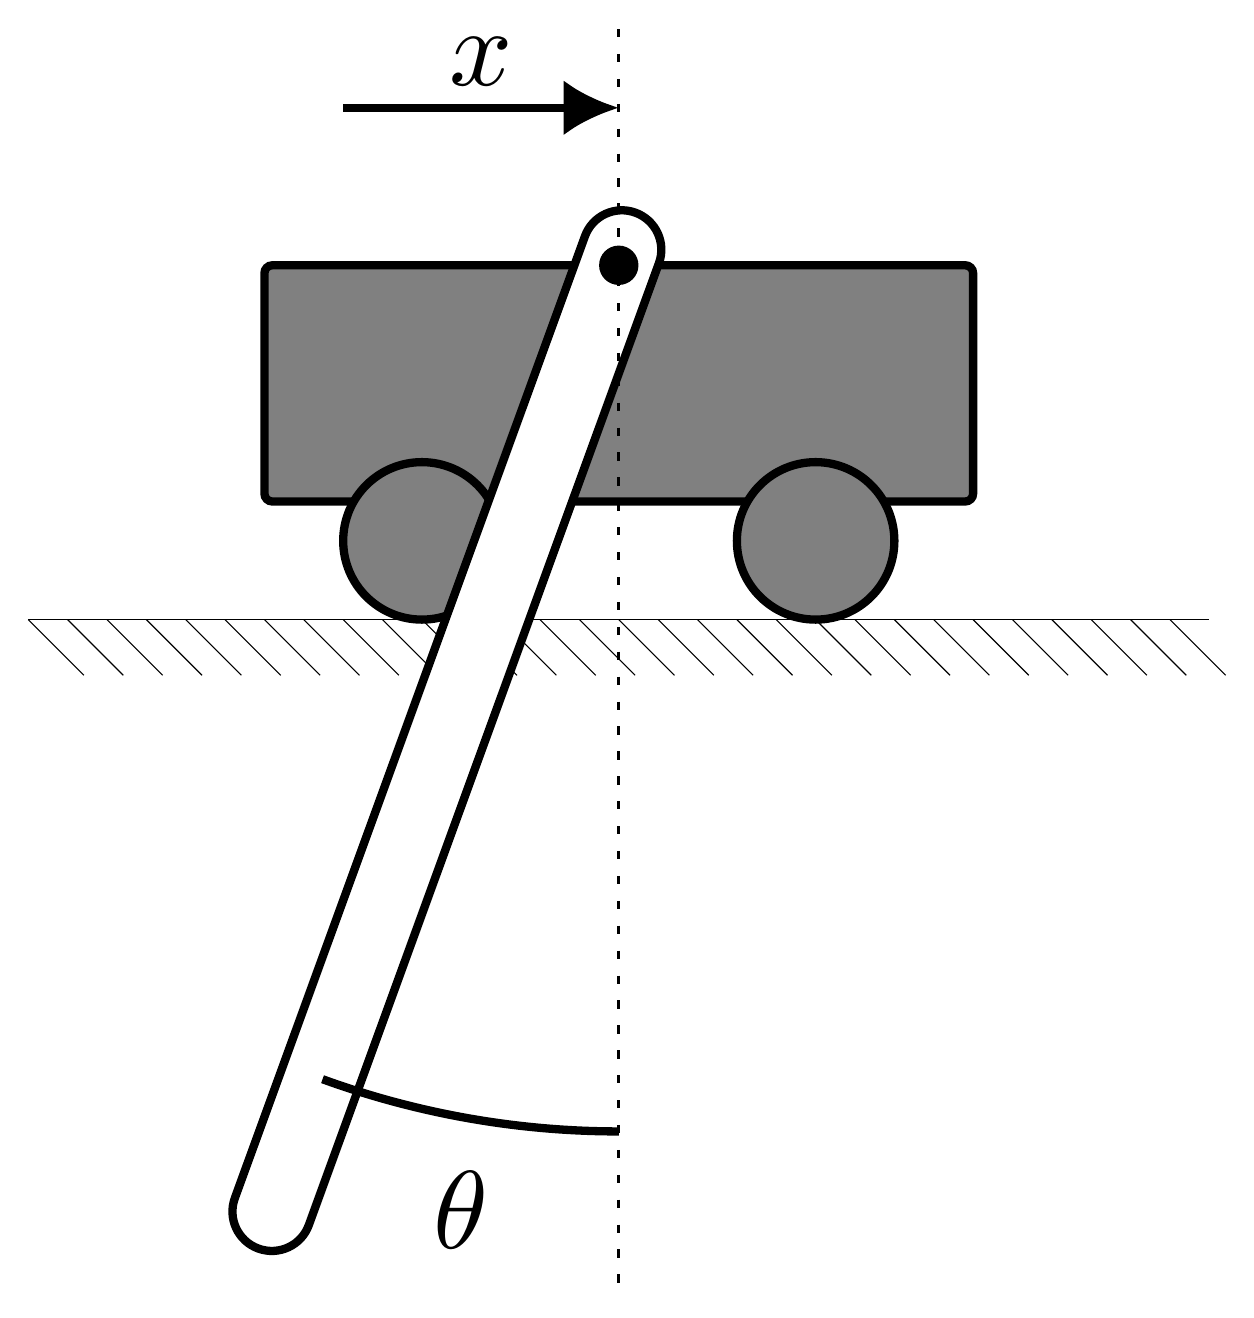
\begin{tikzpicture}[inner sep=0,outer sep=0]

   % Draw decorated 'ground'
   \draw[postaction={draw, decorate, decoration={border, angle=-45,
					amplitude=1cm, segment length=.5cm}}] (-3,-1.5) -- (12,-1.5);

   % The cart
   \draw[draw=black,fill=black!50,draw=black,line width=3pt,rounded corners=1mm] (0,0) rectangle (9cm,3cm);
   \node[fill=black,circle,minimum size=.5cm] (dot) at (4.5cm,3cm) {};

   % Wheels
   \node[fill=white,draw=black,line width=3pt,circle,minimum size=2cm,,fill=black!50] at (2cm,-.5cm) {};
   \node[fill=white,draw=black,line width=3pt,circle,minimum size=2cm,fill=black!50] at (7cm,-.5cm) {};

   % The arm
   \node[anchor=north,minimum width=1cm,minimum height=14cm,draw=black,rotate=-20,rounded corners=5mm,yshift=7mm,xshift=-.3mm,fill=white,draw=black,line width=3pt] at (dot) {};
   \node[fill=black,circle,minimum size=.5cm] at (dot) {};

   % Markings
   \draw[loosely dashed,line width=1pt] (4.5,6) -- (4.5,-10);

   % Arrow
   \draw[->,black,line width=3pt,-{Latex[length=7mm,width=7mm]}] (1,5) --node[above,outer sep=8pt]{\scalebox{4}{$x$}} (4.5,5);

   \def\centerarc[#1](#2)(#3:#4:#5)% Syntax: [draw options] (center) (initial angle:final angle:radius)
   { \draw[#1] ($(#2)+({#5*cos(#3)},{#5*sin(#3)})$) arc (#3:#4:#5); }

   % Draw arc
   \centerarc[black,line width=3pt](dot)(250:270:11)
   \node at (2.5,-9) {\scalebox{4}{$\theta$}};

   %\node[white,minimum size=1cm] at (4.5,-13) {};

 \end{tikzpicture}}\\[2em]~
 \end{subfigure}
 \hfill
 \begin{subfigure}[c]{.7\textwidth}
   \raggedleft\scriptsize
   \setlength{\figurewidth}{\textwidth}
   \setlength{\figureheight}{.55\figurewidth}
   \pgfplotsset{axis on top,ymajorgrids,axis line style={draw=none},legend style={at={(-.1,-.1)},anchor=south east}}
   \pgfplotsset{grid style={line width=.1pt, draw=gray!10,densely dotted}}
   \hspace*{-1.7cm}%
   \def\our{{\sc sfr} (ours)}
   % This file was created with tikzplotlib v0.10.1.
\begin{tikzpicture}

\definecolor{darkgray176}{RGB}{176,176,176}
\definecolor{darkturquoise0191191}{RGB}{0,191,191}
\definecolor{darkviolet1910191}{RGB}{191,0,191}
\definecolor{goldenrod1911910}{RGB}{191,191,0}
\definecolor{green01270}{RGB}{0,127,0}
\definecolor{lightgray204}{RGB}{204,204,204}

\begin{axis}[
height=\figureheight,
legend cell align={left},
legend style={
  fill opacity=0.8,
  draw opacity=1,
  text opacity=1,
  %at={(0.09,0.5)},
  % anchor=west,
  draw=lightgray204
},
tick align=outside,
tick pos=left,
width=\figurewidth,
x grid style={darkgray176},
xlabel={Episode},
xmin=0, xmax=50,
xtick style={color=black},
y grid style={darkgray176},
ylabel={Return},
ymin=-20.6761803239654, ymax=434.199786803273,
ytick style={color=black}
]
\path [draw=darkturquoise0191191, fill=darkturquoise0191191, opacity=0.1]
(axis cs:0,13.428179350054)
--(axis cs:0,7.30889131172923)
--(axis cs:1,9.28755213349604)
--(axis cs:2,14.5760960686498)
--(axis cs:3,15.5060691996425)
--(axis cs:4,18.2928680075549)
--(axis cs:5,24.5898086352006)
--(axis cs:6,30.3040608842919)
--(axis cs:7,41.9959181193707)
--(axis cs:8,53.8732289315574)
--(axis cs:9,72.6987540063586)
--(axis cs:10,88.1409245197496)
--(axis cs:11,104.061319507981)
--(axis cs:12,128.199031598055)
--(axis cs:13,152.941689346881)
--(axis cs:14,181.496732076402)
--(axis cs:15,189.822200712206)
--(axis cs:16,207.754817535136)
--(axis cs:17,218.45130801388)
--(axis cs:18,229.180021771323)
--(axis cs:19,245.019363525644)
--(axis cs:20,244.603047801999)
--(axis cs:21,237.110537908189)
--(axis cs:22,237.283252962022)
--(axis cs:23,243.501749170314)
--(axis cs:24,255.641410555679)
--(axis cs:25,271.088614167502)
--(axis cs:26,271.450223410308)
--(axis cs:27,275.814946458105)
--(axis cs:28,291.110207523579)
--(axis cs:29,307.107143760998)
--(axis cs:30,318.113799076267)
--(axis cs:31,334.94648362165)
--(axis cs:32,340.932730267005)
--(axis cs:33,351.773508875753)
--(axis cs:34,357.442447389532)
--(axis cs:35,360.806765871967)
--(axis cs:36,349.314653969526)
--(axis cs:37,355.07193890814)
--(axis cs:38,358.636450143097)
--(axis cs:39,362.474226260608)
--(axis cs:40,360.345082079734)
--(axis cs:41,360.888678577473)
--(axis cs:42,366.886366220473)
--(axis cs:43,366.826995225648)
--(axis cs:44,380.181108699935)
--(axis cs:45,378.416343311585)
--(axis cs:46,376.346627059407)
--(axis cs:47,377.501758546332)
--(axis cs:48,380.121484570252)
--(axis cs:49,376.02874036263)
--(axis cs:50,375.502145804818)
--(axis cs:51,376.922404302564)
--(axis cs:52,375.717880608245)
--(axis cs:53,377.139922903233)
--(axis cs:54,379.999682054425)
--(axis cs:55,380.01870249647)
--(axis cs:56,379.13494555108)
--(axis cs:57,382.742988307248)
--(axis cs:58,383.057644385398)
--(axis cs:59,382.25231802656)
--(axis cs:60,383.577905148343)
--(axis cs:61,383.159678434199)
--(axis cs:61,395.390236116582)
--(axis cs:61,395.390236116582)
--(axis cs:60,395.431382876559)
--(axis cs:59,394.800193570119)
--(axis cs:58,394.584562951028)
--(axis cs:57,393.861281101931)
--(axis cs:56,393.043777593451)
--(axis cs:55,393.411155901968)
--(axis cs:54,393.882689466571)
--(axis cs:53,393.820152475185)
--(axis cs:52,393.881213019685)
--(axis cs:51,395.67471636394)
--(axis cs:50,395.233500252311)
--(axis cs:49,395.866616387859)
--(axis cs:48,396.901994128479)
--(axis cs:47,394.340592985651)
--(axis cs:46,394.759759506755)
--(axis cs:45,396.436922832213)
--(axis cs:44,396.330104221207)
--(axis cs:43,395.459361891051)
--(axis cs:42,395.771379140855)
--(axis cs:41,396.588739940593)
--(axis cs:40,397.215348828469)
--(axis cs:39,397.581955837781)
--(axis cs:38,395.663047079803)
--(axis cs:37,396.351398646792)
--(axis cs:36,394.893494986773)
--(axis cs:35,396.126191586529)
--(axis cs:34,395.327407346796)
--(axis cs:33,390.589975316142)
--(axis cs:32,387.408020618005)
--(axis cs:31,385.637201681085)
--(axis cs:30,376.169530315213)
--(axis cs:29,367.285583518665)
--(axis cs:28,348.902140365367)
--(axis cs:27,342.754083254572)
--(axis cs:26,337.106287228883)
--(axis cs:25,334.457797060678)
--(axis cs:24,329.988007722061)
--(axis cs:23,323.955471384037)
--(axis cs:22,320.215200273604)
--(axis cs:21,321.932188703903)
--(axis cs:20,328.472527072879)
--(axis cs:19,326.398737594351)
--(axis cs:18,314.241958895791)
--(axis cs:17,297.54124970249)
--(axis cs:16,281.082484386708)
--(axis cs:15,259.116357389448)
--(axis cs:14,243.044882551437)
--(axis cs:13,210.739425135999)
--(axis cs:12,180.843924944914)
--(axis cs:11,149.376511798477)
--(axis cs:10,124.379338448791)
--(axis cs:9,101.316824716595)
--(axis cs:8,86.3775537251123)
--(axis cs:7,72.5978980894687)
--(axis cs:6,56.5076104442527)
--(axis cs:5,48.5394503610476)
--(axis cs:4,38.1261999295808)
--(axis cs:3,26.0627344743401)
--(axis cs:2,20.8633832049079)
--(axis cs:1,15.1199406054661)
--(axis cs:0,13.428179350054)
--cycle;

\path [draw=red, fill=red, opacity=0.1]
(axis cs:0,6.81487478061677)
--(axis cs:0,3.63576139763831)
--(axis cs:1,6.93310499529475)
--(axis cs:2,7.53622719838196)
--(axis cs:3,9.48657165499816)
--(axis cs:4,14.4310047402109)
--(axis cs:5,17.5618756765938)
--(axis cs:6,22.124223284806)
--(axis cs:7,24.8016231337186)
--(axis cs:8,34.551672640224)
--(axis cs:9,40.559663433314)
--(axis cs:10,43.6489080634535)
--(axis cs:11,48.5723301630306)
--(axis cs:12,51.5329642988839)
--(axis cs:13,58.8501221023779)
--(axis cs:14,66.1937104244063)
--(axis cs:15,70.990061191187)
--(axis cs:16,68.9679474398576)
--(axis cs:17,69.260766985767)
--(axis cs:18,79.8999631311463)
--(axis cs:19,86.6200314508851)
--(axis cs:20,85.7787410367239)
--(axis cs:21,95.8936232504671)
--(axis cs:22,108.902600632004)
--(axis cs:23,123.173706573101)
--(axis cs:24,135.76901917715)
--(axis cs:25,150.71052110651)
--(axis cs:26,164.823324603135)
--(axis cs:27,184.083525834446)
--(axis cs:28,211.403863526967)
--(axis cs:29,230.041324429908)
--(axis cs:30,237.812985858024)
--(axis cs:31,242.243317337864)
--(axis cs:32,269.551357927957)
--(axis cs:33,292.927671441866)
--(axis cs:34,310.849318800088)
--(axis cs:35,324.302304794292)
--(axis cs:36,327.913039924009)
--(axis cs:37,322.005982391498)
--(axis cs:38,333.332351575736)
--(axis cs:39,348.818967068055)
--(axis cs:40,349.620124254805)
--(axis cs:41,352.401441643378)
--(axis cs:42,355.450418401524)
--(axis cs:43,352.146541576131)
--(axis cs:44,362.248350138902)
--(axis cs:45,380.122758186299)
--(axis cs:46,384.088167697976)
--(axis cs:47,387.032156204171)
--(axis cs:48,385.316061319519)
--(axis cs:49,384.568446136443)
--(axis cs:50,382.805199507922)
--(axis cs:51,380.395934787242)
--(axis cs:52,378.066020879252)
--(axis cs:53,375.242782265163)
--(axis cs:54,372.149595143965)
--(axis cs:55,368.348813624733)
--(axis cs:56,368.829333707634)
--(axis cs:57,368.037434276356)
--(axis cs:58,368.23269583505)
--(axis cs:59,369.60004277161)
--(axis cs:60,365.768373734385)
--(axis cs:61,365.703036449676)
--(axis cs:62,365.128458879234)
--(axis cs:63,366.641945818317)
--(axis cs:64,365.854883201198)
--(axis cs:65,367.433810490061)
--(axis cs:66,365.592396565988)
--(axis cs:67,366.738529137986)
--(axis cs:68,368.850784210366)
--(axis cs:69,363.433745498677)
--(axis cs:70,359.650300429893)
--(axis cs:71,361.914134203969)
--(axis cs:72,363.128549165492)
--(axis cs:73,360.636288738439)
--(axis cs:73,387.878255939295)
--(axis cs:73,387.878255939295)
--(axis cs:72,389.944110136266)
--(axis cs:71,388.49889832777)
--(axis cs:70,385.932791305947)
--(axis cs:69,386.799919967631)
--(axis cs:68,389.988110442954)
--(axis cs:67,386.914243383987)
--(axis cs:66,385.306886270926)
--(axis cs:65,383.592236262869)
--(axis cs:64,381.470916359349)
--(axis cs:63,381.043962689984)
--(axis cs:62,379.426762678383)
--(axis cs:61,378.062959338898)
--(axis cs:60,376.009572737783)
--(axis cs:59,378.593969679562)
--(axis cs:58,381.643021328036)
--(axis cs:57,384.988734546887)
--(axis cs:56,388.407713106331)
--(axis cs:55,390.272264866478)
--(axis cs:54,395.721983835527)
--(axis cs:53,397.83793367722)
--(axis cs:52,400.22697228481)
--(axis cs:51,401.410779079946)
--(axis cs:50,400.641074295789)
--(axis cs:49,402.25840475467)
--(axis cs:48,404.172158895325)
--(axis cs:47,405.263806320243)
--(axis cs:46,405.25892245095)
--(axis cs:45,405.783662712138)
--(axis cs:44,405.714494709731)
--(axis cs:43,407.532674427287)
--(axis cs:42,409.251359247402)
--(axis cs:41,410.966650702813)
--(axis cs:40,412.72050837459)
--(axis cs:39,413.523606479308)
--(axis cs:38,401.805643571969)
--(axis cs:37,394.15749645982)
--(axis cs:36,390.212201164858)
--(axis cs:35,382.828350875874)
--(axis cs:34,375.117050828818)
--(axis cs:33,364.777380743192)
--(axis cs:32,353.426930341086)
--(axis cs:31,338.763385085231)
--(axis cs:30,338.46039098829)
--(axis cs:29,333.037493319115)
--(axis cs:28,324.992776487681)
--(axis cs:27,299.532932629223)
--(axis cs:26,288.261058312362)
--(axis cs:25,280.276835079403)
--(axis cs:24,262.622555110265)
--(axis cs:23,249.726963383107)
--(axis cs:22,235.292288865753)
--(axis cs:21,224.00861831333)
--(axis cs:20,206.378251351048)
--(axis cs:19,203.129129434926)
--(axis cs:18,187.438490090175)
--(axis cs:17,169.116879341252)
--(axis cs:16,170.210503311447)
--(axis cs:15,169.461452552214)
--(axis cs:14,149.929727194803)
--(axis cs:13,133.403991214158)
--(axis cs:12,122.458682586988)
--(axis cs:11,117.619976260157)
--(axis cs:10,108.331404808479)
--(axis cs:9,99.0645792062276)
--(axis cs:8,85.3013117404981)
--(axis cs:7,65.0900200089816)
--(axis cs:6,56.9843653630364)
--(axis cs:5,45.9907392983818)
--(axis cs:4,38.5924541220938)
--(axis cs:3,28.4432422783743)
--(axis cs:2,19.9809871296687)
--(axis cs:1,14.776997354225)
--(axis cs:0,6.81487478061677)
--cycle;

\path [draw=green01270, fill=green01270, opacity=0.1]
(axis cs:0,5.99461245083012)
--(axis cs:0,2.81149446225963)
--(axis cs:1,2.9837219122176)
--(axis cs:2,2.54154348134139)
--(axis cs:3,2.27081100106255)
--(axis cs:4,3.10088411740579)
--(axis cs:5,4.76007814247754)
--(axis cs:6,7.8209500285014)
--(axis cs:7,13.9778360324578)
--(axis cs:8,18.3936352464216)
--(axis cs:9,24.6544902423307)
--(axis cs:10,31.3619694008475)
--(axis cs:11,35.3901350520787)
--(axis cs:12,42.2593775736581)
--(axis cs:13,52.4053832604296)
--(axis cs:14,62.3631154634491)
--(axis cs:15,63.3844957838641)
--(axis cs:16,67.0473567489912)
--(axis cs:17,70.4655911210402)
--(axis cs:18,74.6902603099488)
--(axis cs:19,80.60939254355)
--(axis cs:20,86.2497897062847)
--(axis cs:21,90.0339135781303)
--(axis cs:22,87.3050110634478)
--(axis cs:23,108.25260327915)
--(axis cs:24,115.882595652148)
--(axis cs:25,124.488189793689)
--(axis cs:26,139.181945821654)
--(axis cs:27,153.139530033028)
--(axis cs:28,151.205456104707)
--(axis cs:29,154.208591554145)
--(axis cs:30,163.119321983175)
--(axis cs:31,167.699525144116)
--(axis cs:32,181.432504039739)
--(axis cs:33,192.454761267538)
--(axis cs:34,196.69121650929)
--(axis cs:35,201.457087868644)
--(axis cs:36,219.242538612505)
--(axis cs:37,230.629118609248)
--(axis cs:38,236.593559450014)
--(axis cs:39,235.81092929979)
--(axis cs:40,235.642370602897)
--(axis cs:41,227.063685874376)
--(axis cs:42,218.736671055354)
--(axis cs:43,207.781066124007)
--(axis cs:44,206.093665841292)
--(axis cs:45,205.162616415751)
--(axis cs:46,206.167404971673)
--(axis cs:47,209.524019300799)
--(axis cs:48,209.157524291902)
--(axis cs:49,219.285468457921)
--(axis cs:50,229.050074936483)
--(axis cs:51,237.496295301312)
--(axis cs:52,237.964422748491)
--(axis cs:53,238.249154429301)
--(axis cs:54,238.154636825253)
--(axis cs:55,236.845295086815)
--(axis cs:56,236.534145241607)
--(axis cs:57,237.006341957755)
--(axis cs:58,236.083195099701)
--(axis cs:59,235.49037911521)
--(axis cs:60,235.237784541299)
--(axis cs:61,235.108123549557)
--(axis cs:62,234.835560327262)
--(axis cs:63,237.788829620684)
--(axis cs:64,237.824200433168)
--(axis cs:65,236.842593243083)
--(axis cs:66,237.036179562796)
--(axis cs:67,235.025029171185)
--(axis cs:68,233.83645118435)
--(axis cs:69,232.983346489038)
--(axis cs:70,232.414694750076)
--(axis cs:71,224.461180505835)
--(axis cs:72,219.012480710855)
--(axis cs:73,215.431016783442)
--(axis cs:74,214.016361819699)
--(axis cs:75,213.367811516068)
--(axis cs:76,212.111061917792)
--(axis cs:77,209.96526716832)
--(axis cs:78,208.410105537933)
--(axis cs:79,213.096584526165)
--(axis cs:80,217.722758901227)
--(axis cs:81,221.671988279191)
--(axis cs:82,223.754567124622)
--(axis cs:83,227.268128291803)
--(axis cs:84,227.714526627746)
--(axis cs:85,227.722452754749)
--(axis cs:86,227.915006261815)
--(axis cs:87,225.004748915991)
--(axis cs:88,223.270175291738)
--(axis cs:89,223.11452189513)
--(axis cs:90,220.490434779552)
--(axis cs:91,218.05900169983)
--(axis cs:92,218.033871061946)
--(axis cs:93,218.245288066081)
--(axis cs:94,219.459753715595)
--(axis cs:95,222.355004437799)
--(axis cs:96,227.605743674264)
--(axis cs:97,226.243400860787)
--(axis cs:98,229.793317116733)
--(axis cs:99,232.990432589255)
--(axis cs:100,236.741331953907)
--(axis cs:101,238.675774603962)
--(axis cs:102,242.800024879119)
--(axis cs:103,246.06975456029)
--(axis cs:104,246.619055922523)
--(axis cs:105,255.520183632938)
--(axis cs:106,257.079472091841)
--(axis cs:107,261.617891670841)
--(axis cs:108,264.453668345715)
--(axis cs:109,270.591897901785)
--(axis cs:110,276.247923548055)
--(axis cs:111,283.283643196874)
--(axis cs:112,289.80372716471)
--(axis cs:113,292.674541189568)
--(axis cs:114,297.620474609947)
--(axis cs:115,301.33824004893)
--(axis cs:116,302.665935700096)
--(axis cs:117,305.608966734389)
--(axis cs:118,308.720128607532)
--(axis cs:119,307.771844009098)
--(axis cs:120,305.387282268855)
--(axis cs:121,300.534219783219)
--(axis cs:122,303.900706917289)
--(axis cs:123,302.70162251079)
--(axis cs:124,305.280171621631)
--(axis cs:125,306.383823818735)
--(axis cs:126,301.154625279878)
--(axis cs:127,306.674156493123)
--(axis cs:128,306.680094787876)
--(axis cs:129,307.188140742304)
--(axis cs:130,310.632051380924)
--(axis cs:131,316.497454608469)
--(axis cs:132,315.423232767986)
--(axis cs:133,319.605338582003)
--(axis cs:134,327.514221132156)
--(axis cs:135,332.618905843438)
--(axis cs:136,340.172317406956)
--(axis cs:137,347.184705449713)
--(axis cs:138,348.370186748524)
--(axis cs:139,348.873999335381)
--(axis cs:140,349.628692358169)
--(axis cs:141,355.201449816715)
--(axis cs:142,359.31424159158)
--(axis cs:143,359.262022531915)
--(axis cs:144,356.149641733415)
--(axis cs:145,358.985319136548)
--(axis cs:146,359.538917403489)
--(axis cs:147,359.835759294755)
--(axis cs:148,365.989546543612)
--(axis cs:148,390.246712916837)
--(axis cs:148,390.246712916837)
--(axis cs:147,387.503139936202)
--(axis cs:146,386.74682630989)
--(axis cs:145,386.134785843921)
--(axis cs:144,385.199207753889)
--(axis cs:143,386.173129140448)
--(axis cs:142,387.060802658908)
--(axis cs:141,386.853382641781)
--(axis cs:140,383.417769128647)
--(axis cs:139,383.630944512275)
--(axis cs:138,384.081041583996)
--(axis cs:137,384.143436334955)
--(axis cs:136,381.400774481472)
--(axis cs:135,380.507492624579)
--(axis cs:134,379.226218473557)
--(axis cs:133,378.337258616483)
--(axis cs:132,382.39186656673)
--(axis cs:131,383.244098125906)
--(axis cs:130,382.746422282406)
--(axis cs:129,382.877764256475)
--(axis cs:128,383.945338561734)
--(axis cs:127,384.125417786662)
--(axis cs:126,383.005225031402)
--(axis cs:125,384.022941165396)
--(axis cs:124,383.68090397041)
--(axis cs:123,383.604564928175)
--(axis cs:122,385.888849204537)
--(axis cs:121,387.344466740219)
--(axis cs:120,388.457506854681)
--(axis cs:119,389.66850480682)
--(axis cs:118,391.416577935437)
--(axis cs:117,391.404303834459)
--(axis cs:116,389.355535704933)
--(axis cs:115,388.617873384908)
--(axis cs:114,386.291991057778)
--(axis cs:113,383.284819696052)
--(axis cs:112,381.822636589562)
--(axis cs:111,376.512702704616)
--(axis cs:110,373.907460134196)
--(axis cs:109,371.920699372996)
--(axis cs:108,371.065135250782)
--(axis cs:107,371.433825705868)
--(axis cs:106,370.095101806474)
--(axis cs:105,369.205783392819)
--(axis cs:104,365.519118134484)
--(axis cs:103,369.607349626722)
--(axis cs:102,367.481946289399)
--(axis cs:101,365.951897210003)
--(axis cs:100,363.562100129223)
--(axis cs:99,360.065018040933)
--(axis cs:98,359.187993441586)
--(axis cs:97,358.96370735073)
--(axis cs:96,360.901408787742)
--(axis cs:95,357.332802263861)
--(axis cs:94,354.21963318626)
--(axis cs:93,353.267512245961)
--(axis cs:92,354.062978761052)
--(axis cs:91,354.591143449401)
--(axis cs:90,355.495357475849)
--(axis cs:89,356.017523946087)
--(axis cs:88,356.36196629838)
--(axis cs:87,358.769320440927)
--(axis cs:86,361.747132629405)
--(axis cs:85,363.382238798367)
--(axis cs:84,363.798664762292)
--(axis cs:83,363.485212405485)
--(axis cs:82,360.625158975346)
--(axis cs:81,360.439547436866)
--(axis cs:80,357.972314202678)
--(axis cs:79,353.294253548519)
--(axis cs:78,350.965099764306)
--(axis cs:77,352.138010920249)
--(axis cs:76,355.468841517915)
--(axis cs:75,357.917825981834)
--(axis cs:74,360.248919786022)
--(axis cs:73,363.722086782728)
--(axis cs:72,369.256771517882)
--(axis cs:71,376.305334868348)
--(axis cs:70,384.706298077339)
--(axis cs:69,386.127079960738)
--(axis cs:68,388.028433192176)
--(axis cs:67,389.773474895283)
--(axis cs:66,392.615557841074)
--(axis cs:65,392.224476192037)
--(axis cs:64,393.714296919432)
--(axis cs:63,393.657947150861)
--(axis cs:62,392.360937780648)
--(axis cs:61,392.864923325443)
--(axis cs:60,392.98201221163)
--(axis cs:59,393.448816136255)
--(axis cs:58,394.506712737213)
--(axis cs:57,395.929575705819)
--(axis cs:56,395.203003806245)
--(axis cs:55,395.755461749123)
--(axis cs:54,397.888106094669)
--(axis cs:53,397.843522877828)
--(axis cs:52,397.294782878951)
--(axis cs:51,396.404766710406)
--(axis cs:50,385.192642043498)
--(axis cs:49,375.224416185633)
--(axis cs:48,366.859422119231)
--(axis cs:47,367.117481553693)
--(axis cs:46,364.142836727545)
--(axis cs:45,362.573337868917)
--(axis cs:44,364.107913443376)
--(axis cs:43,366.800191505388)
--(axis cs:42,375.219560634099)
--(axis cs:41,382.116729469862)
--(axis cs:40,393.242294314095)
--(axis cs:39,393.562450216812)
--(axis cs:38,394.822601133482)
--(axis cs:37,388.273010564031)
--(axis cs:36,373.797684890608)
--(axis cs:35,350.911636382149)
--(axis cs:34,343.506449086718)
--(axis cs:33,337.587693452005)
--(axis cs:32,323.452327055003)
--(axis cs:31,305.858532307132)
--(axis cs:30,299.216269952936)
--(axis cs:29,288.045818855782)
--(axis cs:28,282.876332387496)
--(axis cs:27,277.891576772774)
--(axis cs:26,261.456768253434)
--(axis cs:25,242.06992964639)
--(axis cs:24,223.85068700929)
--(axis cs:23,208.77291323086)
--(axis cs:22,185.594400710234)
--(axis cs:21,177.392950282954)
--(axis cs:20,166.238971814101)
--(axis cs:19,155.135776905303)
--(axis cs:18,139.182567982898)
--(axis cs:17,130.04339954821)
--(axis cs:16,123.481834077425)
--(axis cs:15,117.621168660106)
--(axis cs:14,113.877468147086)
--(axis cs:13,94.2090074942701)
--(axis cs:12,76.3268335474242)
--(axis cs:11,64.3704654790225)
--(axis cs:10,55.949227081334)
--(axis cs:9,44.5422189673499)
--(axis cs:8,33.9405283776266)
--(axis cs:7,24.7665664297862)
--(axis cs:6,14.0269014922753)
--(axis cs:5,11.2280558184848)
--(axis cs:4,9.97529418893538)
--(axis cs:3,7.87922618627532)
--(axis cs:2,6.23063808322809)
--(axis cs:1,6.92791364161922)
--(axis cs:0,5.99461245083012)
--cycle;

\path [draw=darkviolet1910191, fill=darkviolet1910191, opacity=0.1]
(axis cs:0,1.39356748546551)
--(axis cs:0,0.241824417458069)
--(axis cs:1,0.769550938381564)
--(axis cs:2,1.61940607628596)
--(axis cs:3,5.04397897824172)
--(axis cs:4,6.0079305326267)
--(axis cs:5,6.59791470115701)
--(axis cs:6,9.70101748228766)
--(axis cs:7,12.5047063063984)
--(axis cs:8,13.2944962248917)
--(axis cs:9,15.0169028357751)
--(axis cs:10,16.2385294634333)
--(axis cs:11,20.7893519520233)
--(axis cs:12,24.749564458837)
--(axis cs:13,26.9324873756578)
--(axis cs:14,30.3212124235943)
--(axis cs:15,32.3948040082652)
--(axis cs:16,38.2397637344356)
--(axis cs:17,45.1731451634304)
--(axis cs:18,51.43578304352)
--(axis cs:19,52.5578605808246)
--(axis cs:20,51.8962650940394)
--(axis cs:21,54.5397132985593)
--(axis cs:22,53.9340200746088)
--(axis cs:23,62.5532376503928)
--(axis cs:24,67.4117296926621)
--(axis cs:25,74.1965964565979)
--(axis cs:26,80.2005644304067)
--(axis cs:27,88.7212122996431)
--(axis cs:28,104.43228496278)
--(axis cs:29,115.854065400405)
--(axis cs:30,126.163863488488)
--(axis cs:31,129.364380684845)
--(axis cs:32,133.300921731651)
--(axis cs:33,131.037416572851)
--(axis cs:34,134.260226751912)
--(axis cs:35,135.26057969484)
--(axis cs:36,132.312829100295)
--(axis cs:37,132.439458617508)
--(axis cs:38,148.251449491188)
--(axis cs:39,160.652499922675)
--(axis cs:40,173.715524881511)
--(axis cs:41,178.220727293334)
--(axis cs:42,179.348219259212)
--(axis cs:43,181.574198279065)
--(axis cs:44,179.687742331119)
--(axis cs:45,173.104645066771)
--(axis cs:46,159.616625985356)
--(axis cs:47,158.136513644208)
--(axis cs:48,146.479331353504)
--(axis cs:49,162.279791045657)
--(axis cs:50,176.463729180248)
--(axis cs:51,176.756978166363)
--(axis cs:52,180.83573736646)
--(axis cs:53,187.509874475475)
--(axis cs:54,198.111251989307)
--(axis cs:55,189.428745727523)
--(axis cs:56,198.11677577881)
--(axis cs:57,193.792013344711)
--(axis cs:58,185.241412358794)
--(axis cs:59,198.207828305362)
--(axis cs:60,204.997690983488)
--(axis cs:61,213.438284768639)
--(axis cs:62,211.104439717158)
--(axis cs:63,220.731168329645)
--(axis cs:64,221.171317903089)
--(axis cs:65,224.685085903509)
--(axis cs:66,231.265745065277)
--(axis cs:67,231.578953059818)
--(axis cs:68,233.716948493315)
--(axis cs:69,234.976588341593)
--(axis cs:70,237.859012068223)
--(axis cs:71,237.154329814671)
--(axis cs:72,238.350811336514)
--(axis cs:73,237.631290188149)
--(axis cs:74,237.646193804861)
--(axis cs:75,236.73111669247)
--(axis cs:76,237.817975772476)
--(axis cs:77,238.508938695163)
--(axis cs:78,238.713473601489)
--(axis cs:79,239.371852072926)
--(axis cs:80,238.645414100147)
--(axis cs:81,238.76910591274)
--(axis cs:82,238.259694167029)
--(axis cs:83,237.512962326169)
--(axis cs:84,236.399288027393)
--(axis cs:85,234.188984658006)
--(axis cs:86,232.161021961714)
--(axis cs:87,229.959107324382)
--(axis cs:88,228.517649170624)
--(axis cs:89,221.427507175743)
--(axis cs:90,220.768477081534)
--(axis cs:91,220.500512506484)
--(axis cs:92,215.598268360761)
--(axis cs:93,215.842743620866)
--(axis cs:94,217.376127504753)
--(axis cs:95,216.957244596714)
--(axis cs:96,214.805450794544)
--(axis cs:97,221.395637905334)
--(axis cs:98,220.492802787088)
--(axis cs:99,221.473149773267)
--(axis cs:100,226.423818050183)
--(axis cs:101,226.531198245506)
--(axis cs:102,225.137829203583)
--(axis cs:103,225.24221607285)
--(axis cs:104,227.986979679645)
--(axis cs:105,226.412351797152)
--(axis cs:106,219.249462145556)
--(axis cs:107,217.635064888584)
--(axis cs:108,212.816993541227)
--(axis cs:109,203.118824534545)
--(axis cs:110,200.3570747524)
--(axis cs:111,190.114036551943)
--(axis cs:112,190.096366138171)
--(axis cs:113,191.565899336971)
--(axis cs:114,202.102623944396)
--(axis cs:115,202.145544747219)
--(axis cs:116,206.489684813843)
--(axis cs:117,216.014800543256)
--(axis cs:118,217.679248846246)
--(axis cs:119,224.497630683706)
--(axis cs:120,224.743836386768)
--(axis cs:121,225.651294979953)
--(axis cs:122,224.574973856133)
--(axis cs:123,224.064546147887)
--(axis cs:124,225.530486700207)
--(axis cs:125,226.231574023669)
--(axis cs:126,226.146648475491)
--(axis cs:127,223.752992793091)
--(axis cs:128,223.776305745126)
--(axis cs:129,222.81273308559)
--(axis cs:130,227.302194605262)
--(axis cs:131,229.985312893331)
--(axis cs:132,229.007836433297)
--(axis cs:133,226.052400452988)
--(axis cs:134,225.410579769809)
--(axis cs:135,228.630932413035)
--(axis cs:136,220.290542180148)
--(axis cs:137,211.430881351037)
--(axis cs:138,202.3140053011)
--(axis cs:139,201.640190051196)
--(axis cs:140,188.962097551958)
--(axis cs:141,192.58499483454)
--(axis cs:142,195.262860827402)
--(axis cs:143,191.999277095958)
--(axis cs:144,205.423843640838)
--(axis cs:145,214.005177361832)
--(axis cs:146,217.918554525292)
--(axis cs:147,217.12402917933)
--(axis cs:147,347.591682700401)
--(axis cs:147,347.591682700401)
--(axis cs:146,345.041381902778)
--(axis cs:145,338.321114962235)
--(axis cs:144,328.815862684693)
--(axis cs:143,320.95230628951)
--(axis cs:142,335.560637421652)
--(axis cs:141,335.053363090875)
--(axis cs:140,334.244352338179)
--(axis cs:139,345.90454108894)
--(axis cs:138,348.858261849779)
--(axis cs:137,359.267205387549)
--(axis cs:136,367.010872500333)
--(axis cs:135,375.972161687917)
--(axis cs:134,370.084651477139)
--(axis cs:133,370.705268125637)
--(axis cs:132,375.579248038882)
--(axis cs:131,377.233969149649)
--(axis cs:130,373.030866124241)
--(axis cs:129,370.700513915581)
--(axis cs:128,372.345728792666)
--(axis cs:127,374.160495869152)
--(axis cs:126,378.7136755139)
--(axis cs:125,379.136400829846)
--(axis cs:124,378.25260808739)
--(axis cs:123,376.368420465882)
--(axis cs:122,377.061525167305)
--(axis cs:121,378.694034304715)
--(axis cs:120,377.671756569775)
--(axis cs:119,377.161390312387)
--(axis cs:118,366.08513199024)
--(axis cs:117,364.042233186297)
--(axis cs:116,353.253646141662)
--(axis cs:115,348.251268263951)
--(axis cs:114,348.418949503785)
--(axis cs:113,339.310804402195)
--(axis cs:112,336.671266441633)
--(axis cs:111,336.459432514677)
--(axis cs:110,344.038907703807)
--(axis cs:109,346.294029564728)
--(axis cs:108,356.83290927936)
--(axis cs:107,363.613244914425)
--(axis cs:106,365.809240418683)
--(axis cs:105,376.995021440458)
--(axis cs:104,381.126066585003)
--(axis cs:103,376.326469840236)
--(axis cs:102,376.328671650909)
--(axis cs:101,378.866888302346)
--(axis cs:100,379.014270939075)
--(axis cs:99,372.506549170825)
--(axis cs:98,371.738139748312)
--(axis cs:97,372.895889079834)
--(axis cs:96,361.368206145916)
--(axis cs:95,364.918089284664)
--(axis cs:94,365.443736100746)
--(axis cs:93,363.992374196059)
--(axis cs:92,363.778757720324)
--(axis cs:91,369.105806634904)
--(axis cs:90,369.456965900186)
--(axis cs:89,371.235323463143)
--(axis cs:88,384.201138976349)
--(axis cs:87,385.832620886067)
--(axis cs:86,388.561155961011)
--(axis cs:85,391.331594143626)
--(axis cs:84,394.448478038205)
--(axis cs:83,396.247323575854)
--(axis cs:82,397.102219847788)
--(axis cs:81,397.941710995142)
--(axis cs:80,397.645165075802)
--(axis cs:79,398.808570853023)
--(axis cs:78,398.029010598511)
--(axis cs:77,397.742151461869)
--(axis cs:76,396.810913692856)
--(axis cs:75,395.146485130741)
--(axis cs:74,396.610323423623)
--(axis cs:73,396.670231312796)
--(axis cs:72,397.141327725772)
--(axis cs:71,395.17311198199)
--(axis cs:70,396.245501871992)
--(axis cs:69,391.791426575185)
--(axis cs:68,389.924720598267)
--(axis cs:67,387.190573803281)
--(axis cs:66,386.352995278771)
--(axis cs:65,378.568255652086)
--(axis cs:64,374.727432092142)
--(axis cs:63,374.150354850363)
--(axis cs:62,365.348873585836)
--(axis cs:61,366.843386993828)
--(axis cs:60,360.625002888964)
--(axis cs:59,355.875833966138)
--(axis cs:58,348.853793401208)
--(axis cs:57,352.068763628059)
--(axis cs:56,355.984642978629)
--(axis cs:55,351.517863101976)
--(axis cs:54,353.593158086834)
--(axis cs:53,346.838832342152)
--(axis cs:52,338.412338214136)
--(axis cs:51,334.096383058765)
--(axis cs:50,333.928067217915)
--(axis cs:49,327.617295240888)
--(axis cs:48,320.634037872952)
--(axis cs:47,324.934771842014)
--(axis cs:46,326.980036392955)
--(axis cs:45,332.948859114137)
--(axis cs:44,338.717572781948)
--(axis cs:43,340.355574193317)
--(axis cs:42,334.300634614995)
--(axis cs:41,330.799757106462)
--(axis cs:40,323.155481559606)
--(axis cs:39,312.854078188973)
--(axis cs:38,304.207187126473)
--(axis cs:37,295.238413372696)
--(axis cs:36,294.654562581376)
--(axis cs:35,295.922167859939)
--(axis cs:34,295.936208127391)
--(axis cs:33,288.634741286951)
--(axis cs:32,290.378306001961)
--(axis cs:31,284.204295214661)
--(axis cs:30,277.830458620734)
--(axis cs:29,252.443206185059)
--(axis cs:28,224.743641102665)
--(axis cs:27,194.420588247003)
--(axis cs:26,174.868526079008)
--(axis cs:25,161.106608354021)
--(axis cs:24,149.83142502383)
--(axis cs:23,136.614029386045)
--(axis cs:22,114.670151201484)
--(axis cs:21,114.860186947107)
--(axis cs:20,111.874581654313)
--(axis cs:19,120.94334920273)
--(axis cs:18,129.587316521986)
--(axis cs:17,126.116859101878)
--(axis cs:16,109.013307478333)
--(axis cs:15,92.209198515157)
--(axis cs:14,90.1244781844303)
--(axis cs:13,83.9677716661284)
--(axis cs:12,76.2482512693505)
--(axis cs:11,57.9781067848732)
--(axis cs:10,46.524197999812)
--(axis cs:9,44.0506223245375)
--(axis cs:8,40.7202169313316)
--(axis cs:7,37.6785575795765)
--(axis cs:6,29.5757540512016)
--(axis cs:5,23.8087302988239)
--(axis cs:4,21.2733235085682)
--(axis cs:3,19.4798337926018)
--(axis cs:2,10.5628962556385)
--(axis cs:1,3.25154786609231)
--(axis cs:0,1.39356748546551)
--cycle;

\path [draw=goldenrod1911910, fill=goldenrod1911910, opacity=0.1]
(axis cs:0,1.38963595628738)
--(axis cs:0,0)
--(axis cs:1,0)
--(axis cs:2,0)
--(axis cs:3,0)
--(axis cs:4,2.22044604925031e-16)
--(axis cs:5,2.22044604925031e-16)
--(axis cs:6,2.22044604925031e-16)
--(axis cs:7,4.44089209850063e-16)
--(axis cs:8,4.44089209850063e-16)
--(axis cs:9,0)
--(axis cs:10,0.0973525386877547)
--(axis cs:11,0.0973525386877547)
--(axis cs:12,0.0973686580102484)
--(axis cs:13,0.097520135388347)
--(axis cs:14,0.0975177897000039)
--(axis cs:15,0.237414378249012)
--(axis cs:16,0.237292778657729)
--(axis cs:17,0.236997615702925)
--(axis cs:18,0.139108572753573)
--(axis cs:19,0.44475964986838)
--(axis cs:20,0.447022854576367)
--(axis cs:21,0.447876607246815)
--(axis cs:22,0.447895279625472)
--(axis cs:23,0.307743620867702)
--(axis cs:24,0.30770352203302)
--(axis cs:25,0.308095627210658)
--(axis cs:26,0.308367701874595)
--(axis cs:27,0)
--(axis cs:28,0.369230084262199)
--(axis cs:29,0.631231068469607)
--(axis cs:30,0.631940143659889)
--(axis cs:31,1.17552040266445)
--(axis cs:32,1.29232200412051)
--(axis cs:33,1.85346878885701)
--(axis cs:34,2.13723748185411)
--(axis cs:35,3.24279941376945)
--(axis cs:36,3.5284608762958)
--(axis cs:37,3.54401095972215)
--(axis cs:38,4.1355213315782)
--(axis cs:39,3.94878693040711)
--(axis cs:40,4.34045507425287)
--(axis cs:41,4.61015794828907)
--(axis cs:42,5.31541718539844)
--(axis cs:43,5.29898115529169)
--(axis cs:44,5.44519514326062)
--(axis cs:45,6.55466895984959)
--(axis cs:46,7.88517049248746)
--(axis cs:47,8.29298458525354)
--(axis cs:48,9.13197284992191)
--(axis cs:49,10.5590002268828)
--(axis cs:50,11.3881677017845)
--(axis cs:51,11.2167649413722)
--(axis cs:52,11.674945071533)
--(axis cs:53,12.5308397695249)
--(axis cs:54,15.2170394072579)
--(axis cs:55,17.5668148771136)
--(axis cs:56,23.1309814227557)
--(axis cs:57,26.3509103453465)
--(axis cs:58,31.4283342709158)
--(axis cs:59,39.4632911977941)
--(axis cs:60,45.553964491233)
--(axis cs:61,53.1062210169705)
--(axis cs:62,57.145999586077)
--(axis cs:63,62.7227132936143)
--(axis cs:64,66.8143851369584)
--(axis cs:65,70.3342784851486)
--(axis cs:66,71.7207496174059)
--(axis cs:67,74.5309170897552)
--(axis cs:68,77.631759885302)
--(axis cs:69,79.475141659427)
--(axis cs:70,76.2509825654961)
--(axis cs:71,77.8592823429841)
--(axis cs:72,75.5755072700985)
--(axis cs:73,76.5462599869496)
--(axis cs:74,79.6587582970814)
--(axis cs:75,81.2069622375462)
--(axis cs:76,83.1463476479415)
--(axis cs:77,80.8353848695625)
--(axis cs:78,87.9006155245908)
--(axis cs:79,89.1628487400461)
--(axis cs:80,94.1624040660212)
--(axis cs:81,98.1917255021653)
--(axis cs:82,102.055880667071)
--(axis cs:83,103.306646553921)
--(axis cs:84,103.602740404712)
--(axis cs:85,110.496694472372)
--(axis cs:86,117.092930301302)
--(axis cs:87,122.942174898429)
--(axis cs:88,127.591950607361)
--(axis cs:89,132.742163247471)
--(axis cs:90,136.052620219724)
--(axis cs:91,139.531051643874)
--(axis cs:92,143.813640748959)
--(axis cs:93,144.966522174758)
--(axis cs:94,144.450006448331)
--(axis cs:95,145.107885226114)
--(axis cs:96,144.909199592148)
--(axis cs:97,143.913579185654)
--(axis cs:98,144.019349254802)
--(axis cs:99,144.808613963237)
--(axis cs:100,144.827049449949)
--(axis cs:101,145.402887908313)
--(axis cs:102,145.28289498014)
--(axis cs:103,145.015110721617)
--(axis cs:104,149.571931990814)
--(axis cs:105,151.474964159298)
--(axis cs:106,155.160694479578)
--(axis cs:107,156.621798573416)
--(axis cs:108,157.300078900249)
--(axis cs:109,158.841353424569)
--(axis cs:110,158.918130521177)
--(axis cs:111,161.555550496417)
--(axis cs:112,159.248499501643)
--(axis cs:113,158.600728391073)
--(axis cs:114,155.62778455765)
--(axis cs:115,154.058766296402)
--(axis cs:116,155.005776205656)
--(axis cs:117,156.245081981181)
--(axis cs:118,158.298155953457)
--(axis cs:119,157.603191254339)
--(axis cs:120,160.504454853415)
--(axis cs:121,162.518102105812)
--(axis cs:122,162.704556618642)
--(axis cs:123,165.703436393982)
--(axis cs:124,167.938978225861)
--(axis cs:125,168.646088428344)
--(axis cs:126,171.185470292905)
--(axis cs:127,174.271019229163)
--(axis cs:128,171.809420225651)
--(axis cs:129,172.817572910331)
--(axis cs:130,176.187790265794)
--(axis cs:131,175.491571512424)
--(axis cs:132,176.56264101765)
--(axis cs:133,177.441759327656)
--(axis cs:134,176.33764856646)
--(axis cs:135,170.804235062724)
--(axis cs:136,168.515029364573)
--(axis cs:137,168.245117752701)
--(axis cs:138,166.018519508833)
--(axis cs:139,166.794185111892)
--(axis cs:140,162.767003832468)
--(axis cs:141,164.254014901571)
--(axis cs:142,168.305246840107)
--(axis cs:143,171.122541101695)
--(axis cs:144,178.527326350056)
--(axis cs:145,182.707747926948)
--(axis cs:146,188.016716850543)
--(axis cs:147,190.288685970539)
--(axis cs:148,194.253150174746)
--(axis cs:149,197.693729379401)
--(axis cs:150,201.813645905239)
--(axis cs:151,207.881777106137)
--(axis cs:152,209.548354587472)
--(axis cs:153,212.431865183728)
--(axis cs:154,213.483704914484)
--(axis cs:155,217.021935997564)
--(axis cs:156,219.631106943431)
--(axis cs:157,220.096079321451)
--(axis cs:158,219.565035697668)
--(axis cs:159,220.948538882299)
--(axis cs:160,221.452277097129)
--(axis cs:161,220.965570516239)
--(axis cs:162,222.986025984786)
--(axis cs:163,224.257413473743)
--(axis cs:164,224.701543142528)
--(axis cs:165,225.270644314542)
--(axis cs:166,225.722541973948)
--(axis cs:167,223.652322041983)
--(axis cs:168,223.719799287959)
--(axis cs:169,223.088242185563)
--(axis cs:170,221.551721960122)
--(axis cs:171,221.860997810265)
--(axis cs:172,222.161174666631)
--(axis cs:173,221.251398480256)
--(axis cs:174,221.388767545949)
--(axis cs:175,223.133673032226)
--(axis cs:176,222.70253362448)
--(axis cs:177,223.642774735965)
--(axis cs:178,224.046426153343)
--(axis cs:179,223.626084327498)
--(axis cs:180,223.536211317108)
--(axis cs:181,223.599892469304)
--(axis cs:182,223.106619713792)
--(axis cs:183,223.127039214736)
--(axis cs:184,222.99950781497)
--(axis cs:185,223.096609043845)
--(axis cs:186,223.872237297313)
--(axis cs:187,222.88003329618)
--(axis cs:188,223.014552486453)
--(axis cs:189,223.34825315097)
--(axis cs:190,223.636451354608)
--(axis cs:191,222.085707850107)
--(axis cs:192,221.805192360158)
--(axis cs:193,220.989333899178)
--(axis cs:194,220.324371497256)
--(axis cs:195,221.96798678335)
--(axis cs:196,221.732304639167)
--(axis cs:197,221.194328941816)
--(axis cs:198,221.787736582257)
--(axis cs:199,221.773870610353)
--(axis cs:200,222.183510475614)
--(axis cs:201,222.144158457106)
--(axis cs:202,221.990652569053)
--(axis cs:203,222.177530757405)
--(axis cs:204,221.576616463306)
--(axis cs:205,220.634714716895)
--(axis cs:206,219.135629796257)
--(axis cs:207,220.754843068111)
--(axis cs:208,220.768653259319)
--(axis cs:209,221.171280889953)
--(axis cs:210,221.984381051074)
--(axis cs:211,220.882548420265)
--(axis cs:212,222.174324080665)
--(axis cs:213,221.572125398049)
--(axis cs:214,220.466941228806)
--(axis cs:215,216.442667021741)
--(axis cs:216,212.988720985021)
--(axis cs:217,209.619577635369)
--(axis cs:218,209.561742113407)
--(axis cs:219,209.952651979077)
--(axis cs:220,210.248811032252)
--(axis cs:221,212.93037544289)
--(axis cs:222,215.447505186367)
--(axis cs:223,216.948523316128)
--(axis cs:224,219.239215702804)
--(axis cs:225,222.513005544723)
--(axis cs:226,222.659094083191)
--(axis cs:227,223.133473934301)
--(axis cs:228,223.053747047866)
--(axis cs:229,223.432908041998)
--(axis cs:230,223.818911083103)
--(axis cs:231,226.317372898711)
--(axis cs:232,227.508292453092)
--(axis cs:233,227.66700158944)
--(axis cs:234,227.765724338148)
--(axis cs:235,227.910877519125)
--(axis cs:236,228.04724195468)
--(axis cs:237,228.109692648611)
--(axis cs:238,227.700197483582)
--(axis cs:239,227.881698894079)
--(axis cs:240,228.061512382774)
--(axis cs:241,227.792634133378)
--(axis cs:242,227.721038200442)
--(axis cs:243,227.569187848565)
--(axis cs:244,225.484280576094)
--(axis cs:245,225.017952960258)
--(axis cs:246,225.23309709066)
--(axis cs:247,225.213201554247)
--(axis cs:248,222.098644983367)
--(axis cs:249,221.928762147742)
--(axis cs:250,221.655571124388)
--(axis cs:251,221.324346408886)
--(axis cs:252,223.017046932701)
--(axis cs:253,223.136845075656)
--(axis cs:254,222.737558011259)
--(axis cs:255,222.365366510169)
--(axis cs:256,224.873732289263)
--(axis cs:257,225.135088393785)
--(axis cs:258,225.337023417326)
--(axis cs:259,225.587183652643)
--(axis cs:260,225.754638080952)
--(axis cs:261,225.127111016594)
--(axis cs:262,225.309666503742)
--(axis cs:263,223.33443576845)
--(axis cs:264,222.492408722341)
--(axis cs:265,221.789962961652)
--(axis cs:266,220.369459588263)
--(axis cs:267,218.655583965042)
--(axis cs:268,216.30102570175)
--(axis cs:269,214.491336591068)
--(axis cs:270,213.371052013839)
--(axis cs:271,213.605045976165)
--(axis cs:272,214.007363300038)
--(axis cs:273,213.812289906431)
--(axis cs:274,215.235401717596)
--(axis cs:275,216.22755206127)
--(axis cs:276,217.399327507305)
--(axis cs:277,219.2140328424)
--(axis cs:278,219.919017934245)
--(axis cs:279,221.326056531267)
--(axis cs:280,222.533776301672)
--(axis cs:281,223.370484997248)
--(axis cs:282,223.585111984126)
--(axis cs:283,224.022228827054)
--(axis cs:284,224.816776960346)
--(axis cs:285,225.504343950145)
--(axis cs:286,225.815836706314)
--(axis cs:287,226.237343741299)
--(axis cs:288,225.92441480255)
--(axis cs:289,225.126982650711)
--(axis cs:290,225.376834196698)
--(axis cs:291,225.499544411022)
--(axis cs:292,225.909923302737)
--(axis cs:293,225.6148345017)
--(axis cs:294,225.180497058435)
--(axis cs:295,225.374211043671)
--(axis cs:296,222.891836496799)
--(axis cs:297,222.815270624969)
--(axis cs:298,222.675947618953)
--(axis cs:299,222.054910234559)
--(axis cs:300,221.525595275585)
--(axis cs:301,221.936342894452)
--(axis cs:302,222.086937433701)
--(axis cs:303,221.711504237613)
--(axis cs:304,224.297533503483)
--(axis cs:305,225.381234278387)
--(axis cs:306,225.318002737665)
--(axis cs:307,226.424235716287)
--(axis cs:308,227.823241743938)
--(axis cs:309,228.417099631832)
--(axis cs:310,229.360009433099)
--(axis cs:311,230.136785988555)
--(axis cs:312,230.54437836949)
--(axis cs:313,230.97641242546)
--(axis cs:314,231.637963982156)
--(axis cs:315,231.998357135888)
--(axis cs:316,231.696528611614)
--(axis cs:317,231.525921795114)
--(axis cs:318,231.666395899799)
--(axis cs:319,231.820088381992)
--(axis cs:320,231.858104473589)
--(axis cs:321,232.113152747017)
--(axis cs:322,231.873356326118)
--(axis cs:323,231.781799955832)
--(axis cs:324,231.431098184029)
--(axis cs:325,231.28086394243)
--(axis cs:326,230.934509144581)
--(axis cs:327,230.748439506365)
--(axis cs:328,230.443705494657)
--(axis cs:329,230.323995204414)
--(axis cs:330,230.529961863805)
--(axis cs:331,230.707946823898)
--(axis cs:332,231.226163758743)
--(axis cs:333,231.326480462274)
--(axis cs:334,231.66264794576)
--(axis cs:335,231.63693550178)
--(axis cs:336,231.90686028186)
--(axis cs:337,232.026554743266)
--(axis cs:338,231.901618719035)
--(axis cs:339,231.713658824761)
--(axis cs:340,231.597645786387)
--(axis cs:341,231.395711936156)
--(axis cs:342,231.291022896772)
--(axis cs:343,231.409005246108)
--(axis cs:344,231.485667317936)
--(axis cs:345,231.182218629334)
--(axis cs:346,231.325766839924)
--(axis cs:347,231.422517817537)
--(axis cs:348,231.435414890041)
--(axis cs:349,231.506550813115)
--(axis cs:350,231.810320445544)
--(axis cs:351,231.579486029908)
--(axis cs:352,231.579246893675)
--(axis cs:353,231.830262512512)
--(axis cs:354,231.813081916589)
--(axis cs:355,231.930543773079)
--(axis cs:356,232.047488196786)
--(axis cs:357,232.017433617849)
--(axis cs:358,231.788275320705)
--(axis cs:359,232.009253666591)
--(axis cs:360,231.938620145827)
--(axis cs:361,232.091742632262)
--(axis cs:362,231.816554356451)
--(axis cs:363,231.733122503856)
--(axis cs:364,231.755928434046)
--(axis cs:365,232.021122838997)
--(axis cs:366,231.869962266074)
--(axis cs:367,231.887277755907)
--(axis cs:368,231.885849396247)
--(axis cs:369,231.619183556869)
--(axis cs:370,231.869006162995)
--(axis cs:371,231.870781492677)
--(axis cs:372,231.808812241369)
--(axis cs:373,231.638369438646)
--(axis cs:374,231.788039536821)
--(axis cs:375,231.540651434437)
--(axis cs:376,231.465965115236)
--(axis cs:377,231.839438820879)
--(axis cs:378,231.881909619113)
--(axis cs:379,231.726023602114)
--(axis cs:380,231.693588342085)
--(axis cs:381,231.80559049152)
--(axis cs:382,231.786619368828)
--(axis cs:383,232.004123895585)
--(axis cs:384,232.124318680538)
--(axis cs:385,231.912844271767)
--(axis cs:386,231.880428331808)
--(axis cs:387,232.11923157983)
--(axis cs:388,231.857340144228)
--(axis cs:389,231.770277112592)
--(axis cs:390,231.815299630824)
--(axis cs:391,231.848314399677)
--(axis cs:392,231.699283396223)
--(axis cs:393,231.807992738693)
--(axis cs:394,231.868990675614)
--(axis cs:395,231.608171837105)
--(axis cs:396,232.082345191458)
--(axis cs:397,232.18402035246)
--(axis cs:398,232.174666373344)
--(axis cs:399,232.068708323303)
--(axis cs:400,232.052700206915)
--(axis cs:401,231.791460488182)
--(axis cs:402,231.659908540012)
--(axis cs:403,231.732591548249)
--(axis cs:404,231.461422194643)
--(axis cs:405,231.577084253483)
--(axis cs:406,231.699031274287)
--(axis cs:407,231.920744439791)
--(axis cs:408,231.942708130352)
--(axis cs:409,231.959198089513)
--(axis cs:410,232.054230873801)
--(axis cs:411,232.118289046906)
--(axis cs:412,232.115433579308)
--(axis cs:413,232.076186918543)
--(axis cs:414,231.863588592227)
--(axis cs:415,231.717434413775)
--(axis cs:416,231.869985480285)
--(axis cs:417,231.966955998651)
--(axis cs:418,232.005956312908)
--(axis cs:419,231.951617911072)
--(axis cs:420,231.88352790108)
--(axis cs:421,231.77264220006)
--(axis cs:422,231.871688270339)
--(axis cs:423,231.836785626272)
--(axis cs:424,231.741879484703)
--(axis cs:425,231.674326395424)
--(axis cs:426,231.676851470848)
--(axis cs:427,231.846968855965)
--(axis cs:428,232.017028008141)
--(axis cs:429,232.023817974682)
--(axis cs:430,232.125242573967)
--(axis cs:431,232.144633429884)
--(axis cs:432,232.123737847857)
--(axis cs:433,232.169625751349)
--(axis cs:434,232.130015500722)
--(axis cs:435,231.874175297017)
--(axis cs:436,231.792073267178)
--(axis cs:437,231.722842349041)
--(axis cs:438,231.633640564029)
--(axis cs:439,231.702014418621)
--(axis cs:440,231.833545469549)
--(axis cs:441,231.908099873306)
--(axis cs:442,231.889933168066)
--(axis cs:443,232.036255975763)
--(axis cs:444,231.920796541106)
--(axis cs:445,231.866511266147)
--(axis cs:446,231.803559941592)
--(axis cs:447,231.897981836143)
--(axis cs:448,231.647330108253)
--(axis cs:449,231.47797140316)
--(axis cs:450,231.194677357962)
--(axis cs:451,231.123236600851)
--(axis cs:452,231.33592517965)
--(axis cs:453,231.41731491032)
--(axis cs:454,231.582460027583)
--(axis cs:455,231.53382065768)
--(axis cs:456,231.782057160823)
--(axis cs:457,231.913501524661)
--(axis cs:458,232.216279124674)
--(axis cs:459,232.222733580297)
--(axis cs:460,232.254861067471)
--(axis cs:461,232.347611944577)
--(axis cs:462,232.00380476388)
--(axis cs:463,231.970606717048)
--(axis cs:464,231.66883986981)
--(axis cs:465,231.795546962631)
--(axis cs:466,231.749589609729)
--(axis cs:467,231.948386787751)
--(axis cs:468,231.968113836508)
--(axis cs:469,231.873821344166)
--(axis cs:470,232.253300157856)
--(axis cs:471,232.288501677)
--(axis cs:472,232.56726162258)
--(axis cs:473,232.490566415844)
--(axis cs:474,232.551787933205)
--(axis cs:475,232.481076489527)
--(axis cs:476,232.412584008543)
--(axis cs:477,232.583589963882)
--(axis cs:478,232.553304179092)
--(axis cs:479,232.600329163129)
--(axis cs:480,232.520688572817)
--(axis cs:481,232.362961911187)
--(axis cs:482,232.397370557311)
--(axis cs:483,232.325096196284)
--(axis cs:484,232.404072697118)
--(axis cs:485,232.361823441367)
--(axis cs:486,232.338763211672)
--(axis cs:487,232.26990665784)
--(axis cs:488,232.432006666601)
--(axis cs:489,232.364408876621)
--(axis cs:490,232.181091532231)
--(axis cs:491,232.356045594239)
--(axis cs:492,232.316709546943)
--(axis cs:493,232.225739740816)
--(axis cs:494,232.194920637245)
--(axis cs:495,232.194047215915)
--(axis cs:496,232.214886709598)
--(axis cs:497,232.54347903692)
--(axis cs:498,232.668881736645)
--(axis cs:499,232.391234790938)
--(axis cs:500,232.164416517952)
--(axis cs:501,232.175454709875)
--(axis cs:502,231.729923410226)
--(axis cs:503,231.689115341775)
--(axis cs:504,231.583297089332)
--(axis cs:505,231.375494862912)
--(axis cs:506,231.435594818505)
--(axis cs:507,231.524627611919)
--(axis cs:508,231.484273243402)
--(axis cs:509,231.368042316182)
--(axis cs:510,231.608539173197)
--(axis cs:511,231.374229165933)
--(axis cs:512,231.403939764748)
--(axis cs:513,231.543367520762)
--(axis cs:514,231.182319549907)
--(axis cs:515,231.096769213657)
--(axis cs:516,231.15835770708)
--(axis cs:517,231.012599900148)
--(axis cs:518,231.152011009584)
--(axis cs:519,231.232145618629)
--(axis cs:520,231.145069016989)
--(axis cs:521,230.955287511406)
--(axis cs:522,231.035178992415)
--(axis cs:523,231.264526753037)
--(axis cs:524,230.781712676574)
--(axis cs:525,230.8580801275)
--(axis cs:526,230.731232935843)
--(axis cs:527,230.488003149165)
--(axis cs:528,230.289943828704)
--(axis cs:529,230.00736130334)
--(axis cs:530,230.14349641644)
--(axis cs:531,230.183855197572)
--(axis cs:532,230.555223651199)
--(axis cs:533,230.650844695561)
--(axis cs:534,230.448594425164)
--(axis cs:535,230.39083498237)
--(axis cs:536,230.454754467747)
--(axis cs:537,230.628582429339)
--(axis cs:538,230.822952180843)
--(axis cs:539,230.316349220704)
--(axis cs:540,230.004149819309)
--(axis cs:541,229.688000600049)
--(axis cs:542,229.698794799935)
--(axis cs:543,229.780789238665)
--(axis cs:544,229.791191368796)
--(axis cs:545,229.679266830287)
--(axis cs:546,229.526185900878)
--(axis cs:547,229.726118382941)
--(axis cs:548,229.92642908966)
--(axis cs:549,230.143589039529)
--(axis cs:550,230.229219212828)
--(axis cs:551,230.479204427913)
--(axis cs:552,230.627614517034)
--(axis cs:553,230.959429712303)
--(axis cs:554,230.451890281274)
--(axis cs:555,230.510190329318)
--(axis cs:556,230.46231633342)
--(axis cs:557,230.480131149127)
--(axis cs:558,230.240836617064)
--(axis cs:559,229.967864769072)
--(axis cs:560,230.045109899274)
--(axis cs:561,229.807598613217)
--(axis cs:562,229.863550261541)
--(axis cs:563,229.951290231212)
--(axis cs:564,230.266134959317)
--(axis cs:565,230.49365583847)
--(axis cs:566,230.947416992153)
--(axis cs:567,231.33795097585)
--(axis cs:568,231.061188353642)
--(axis cs:569,231.244198908248)
--(axis cs:570,231.80678043579)
--(axis cs:571,231.71299218896)
--(axis cs:572,231.431522944396)
--(axis cs:573,231.243680411537)
--(axis cs:574,230.86874661942)
--(axis cs:575,230.8512271372)
--(axis cs:576,230.774728776184)
--(axis cs:577,230.487402081626)
--(axis cs:578,230.45643094834)
--(axis cs:579,230.158966482802)
--(axis cs:580,230.46746746806)
--(axis cs:581,230.582318728431)
--(axis cs:582,230.986599108455)
--(axis cs:583,229.428719203216)
--(axis cs:584,229.826285858333)
--(axis cs:585,229.789216110504)
--(axis cs:586,228.667167869569)
--(axis cs:587,229.100798588723)
--(axis cs:588,229.042314465136)
--(axis cs:589,228.994872951124)
--(axis cs:590,228.956225787458)
--(axis cs:591,230.352783167086)
--(axis cs:592,229.515960426024)
--(axis cs:593,229.539237435134)
--(axis cs:594,230.492898012471)
--(axis cs:595,229.973582433998)
--(axis cs:596,230.142439410736)
--(axis cs:597,230.136035485443)
--(axis cs:598,230.120875155193)
--(axis cs:599,230.358576357272)
--(axis cs:600,231.035972168376)
--(axis cs:601,231.349046036798)
--(axis cs:602,231.571526874063)
--(axis cs:603,232.013494039876)
--(axis cs:604,231.874745574341)
--(axis cs:605,232.102525508363)
--(axis cs:606,231.962462901815)
--(axis cs:607,231.682035779597)
--(axis cs:608,231.649176719449)
--(axis cs:609,231.510481849758)
--(axis cs:610,231.229350503387)
--(axis cs:611,231.26609482487)
--(axis cs:612,231.333835103793)
--(axis cs:613,231.292532414855)
--(axis cs:614,231.672973149712)
--(axis cs:615,231.7818028463)
--(axis cs:616,231.799651922172)
--(axis cs:617,232.015344519367)
--(axis cs:618,232.074330181602)
--(axis cs:619,231.942910314731)
--(axis cs:620,231.955208127406)
--(axis cs:621,231.836346571202)
--(axis cs:622,231.584932315788)
--(axis cs:623,231.547062908602)
--(axis cs:624,231.479006267292)
--(axis cs:625,231.33308857122)
--(axis cs:626,231.563282191206)
--(axis cs:627,231.728455456612)
--(axis cs:628,231.72818690317)
--(axis cs:629,231.846542841955)
--(axis cs:630,231.945697856447)
--(axis cs:631,232.120718054987)
--(axis cs:632,232.10980235625)
--(axis cs:633,232.254110688575)
--(axis cs:634,232.115896653559)
--(axis cs:635,232.158471181134)
--(axis cs:636,232.29182317703)
--(axis cs:637,232.125276899061)
--(axis cs:638,232.075721399928)
--(axis cs:639,232.118634456791)
--(axis cs:640,232.379698058142)
--(axis cs:641,232.457716091586)
--(axis cs:642,232.671578590749)
--(axis cs:643,232.558552521134)
--(axis cs:644,232.57092623571)
--(axis cs:645,232.646344714117)
--(axis cs:646,232.56718496832)
--(axis cs:647,232.355064626537)
--(axis cs:648,232.136757066118)
--(axis cs:649,232.019876743173)
--(axis cs:650,231.643304025844)
--(axis cs:651,231.747075233173)
--(axis cs:652,231.602148690504)
--(axis cs:653,231.738929684084)
--(axis cs:654,231.616918492239)
--(axis cs:655,231.722294318519)
--(axis cs:656,231.867017243277)
--(axis cs:657,231.789723477201)
--(axis cs:658,232.073731816052)
--(axis cs:659,232.224864934395)
--(axis cs:660,232.268141572446)
--(axis cs:661,232.020092266029)
--(axis cs:662,232.231954599799)
--(axis cs:663,232.396328645875)
--(axis cs:664,232.45654483383)
--(axis cs:665,232.497823770883)
--(axis cs:666,232.448937219236)
--(axis cs:667,232.385045594782)
--(axis cs:668,232.289870676534)
--(axis cs:669,232.457266004594)
--(axis cs:670,232.580297083354)
--(axis cs:671,232.512944366944)
--(axis cs:672,232.533949723877)
--(axis cs:673,232.595144303477)
--(axis cs:674,232.560097996073)
--(axis cs:675,232.512843222827)
--(axis cs:676,232.5865623124)
--(axis cs:677,232.501070610407)
--(axis cs:678,232.502554112029)
--(axis cs:679,232.427210042128)
--(axis cs:680,232.343101273943)
--(axis cs:681,232.274397494648)
--(axis cs:682,232.236619567848)
--(axis cs:683,232.169479782127)
--(axis cs:684,232.186618076737)
--(axis cs:685,232.28858519875)
--(axis cs:686,232.028259541169)
--(axis cs:687,232.068122628519)
--(axis cs:688,232.087171274614)
--(axis cs:689,232.093451208688)
--(axis cs:690,232.017006324869)
--(axis cs:691,232.093412340521)
--(axis cs:692,232.097053909767)
--(axis cs:693,231.85684715503)
--(axis cs:694,231.994318449045)
--(axis cs:695,231.848194725494)
--(axis cs:696,231.621731647316)
--(axis cs:697,231.549216685188)
--(axis cs:698,231.676473736157)
--(axis cs:699,231.576197075216)
--(axis cs:700,231.410204721614)
--(axis cs:701,231.519766362748)
--(axis cs:702,231.569717068255)
--(axis cs:703,231.69767835868)
--(axis cs:704,231.838114932692)
--(axis cs:705,231.819994502888)
--(axis cs:706,231.797734889146)
--(axis cs:707,231.694244545364)
--(axis cs:708,231.883214131552)
--(axis cs:709,231.938428327193)
--(axis cs:710,231.905190194908)
--(axis cs:711,231.786730187662)
--(axis cs:712,231.829522196098)
--(axis cs:713,231.807379829871)
--(axis cs:714,231.814219495872)
--(axis cs:715,231.973476691957)
--(axis cs:716,231.757052355114)
--(axis cs:717,231.631386455992)
--(axis cs:718,231.550598482681)
--(axis cs:719,231.616253849431)
--(axis cs:720,231.613221879579)
--(axis cs:721,231.740706161896)
--(axis cs:722,231.604952019143)
--(axis cs:723,231.656442551471)
--(axis cs:724,231.86306586519)
--(axis cs:725,232.128759154572)
--(axis cs:726,232.096291129664)
--(axis cs:727,232.071335362851)
--(axis cs:728,231.854500514794)
--(axis cs:729,231.728217245207)
--(axis cs:730,231.904766973014)
--(axis cs:731,231.759489617797)
--(axis cs:732,231.712101458577)
--(axis cs:733,231.595293128878)
--(axis cs:734,231.687672044856)
--(axis cs:735,231.697301691985)
--(axis cs:736,231.824139161167)
--(axis cs:737,231.81830796861)
--(axis cs:738,231.800167106401)
--(axis cs:739,231.808067182762)
--(axis cs:740,231.739534640716)
--(axis cs:741,231.628885373137)
--(axis cs:742,231.590434070054)
--(axis cs:743,231.656167964728)
--(axis cs:744,231.595011555129)
--(axis cs:745,231.7043616851)
--(axis cs:746,231.684681123639)
--(axis cs:747,231.644320166281)
--(axis cs:748,231.727394191815)
--(axis cs:749,231.721535217088)
--(axis cs:750,231.735944677432)
--(axis cs:751,231.786353871364)
--(axis cs:752,231.79902747773)
--(axis cs:753,231.636160204905)
--(axis cs:754,231.679511827503)
--(axis cs:755,231.710828815132)
--(axis cs:756,231.744110152654)
--(axis cs:757,231.794644991701)
--(axis cs:758,231.787809981871)
--(axis cs:759,231.605077517873)
--(axis cs:760,231.711764181139)
--(axis cs:761,231.925353982259)
--(axis cs:762,231.86864326906)
--(axis cs:763,231.877648149655)
--(axis cs:764,231.921827986371)
--(axis cs:765,231.902147344049)
--(axis cs:766,231.882907123763)
--(axis cs:767,232.034094621322)
--(axis cs:768,231.986041303035)
--(axis cs:769,231.722810950177)
--(axis cs:770,231.709327103194)
--(axis cs:771,231.755393675436)
--(axis cs:772,231.562097492216)
--(axis cs:773,231.622869174909)
--(axis cs:774,231.607215436538)
--(axis cs:775,231.610121137448)
--(axis cs:776,231.500508788418)
--(axis cs:777,231.591079854843)
--(axis cs:778,231.649445154275)
--(axis cs:779,231.599355112844)
--(axis cs:780,231.572874517459)
--(axis cs:781,231.570545916513)
--(axis cs:782,231.63511166767)
--(axis cs:783,231.405794801316)
--(axis cs:784,231.491113465765)
--(axis cs:785,231.535056451588)
--(axis cs:786,231.467297161424)
--(axis cs:787,231.53189905417)
--(axis cs:788,231.615096211595)
--(axis cs:789,231.540188100922)
--(axis cs:790,231.390500259994)
--(axis cs:791,231.465217111952)
--(axis cs:792,230.57157094705)
--(axis cs:793,230.779734958771)
--(axis cs:794,230.946891635938)
--(axis cs:795,230.669963799995)
--(axis cs:796,230.759658404821)
--(axis cs:797,230.782537055038)
--(axis cs:798,230.951796543992)
--(axis cs:799,231.041248177593)
--(axis cs:800,231.960036559953)
--(axis cs:801,231.731449652892)
--(axis cs:802,231.653747158851)
--(axis cs:803,231.865467621685)
--(axis cs:804,231.820096627961)
--(axis cs:805,231.860401453554)
--(axis cs:806,231.822925433433)
--(axis cs:807,231.87085160427)
--(axis cs:808,231.896532486946)
--(axis cs:809,232.091191477857)
--(axis cs:810,232.147468394512)
--(axis cs:811,232.180947482434)
--(axis cs:812,232.01938736934)
--(axis cs:813,231.886066529954)
--(axis cs:814,231.789257124112)
--(axis cs:815,231.792365788827)
--(axis cs:816,231.800587676867)
--(axis cs:817,231.579582522604)
--(axis cs:818,231.477405792468)
--(axis cs:819,231.397875217975)
--(axis cs:820,231.352452085163)
--(axis cs:821,231.450275461697)
--(axis cs:822,231.513578278362)
--(axis cs:823,231.464611817354)
--(axis cs:824,231.342569221162)
--(axis cs:825,231.320948099052)
--(axis cs:826,231.272540804977)
--(axis cs:827,231.346671698367)
--(axis cs:828,231.520998186778)
--(axis cs:829,231.686286970323)
--(axis cs:830,231.721159432331)
--(axis cs:831,231.815597457108)
--(axis cs:832,231.934618197064)
--(axis cs:833,232.009987455602)
--(axis cs:834,231.736664823072)
--(axis cs:835,231.634425562262)
--(axis cs:836,231.575719934965)
--(axis cs:837,231.325888253608)
--(axis cs:838,231.392177448452)
--(axis cs:839,231.300042287391)
--(axis cs:840,231.035044644035)
--(axis cs:841,230.991924690648)
--(axis cs:842,231.110581151735)
--(axis cs:843,231.259231015135)
--(axis cs:844,231.351438888112)
--(axis cs:845,231.546965959284)
--(axis cs:846,231.176501457597)
--(axis cs:847,231.077005201354)
--(axis cs:848,231.248956237092)
--(axis cs:849,231.212315901752)
--(axis cs:850,231.422519046408)
--(axis cs:851,231.270363588834)
--(axis cs:852,231.064085528238)
--(axis cs:853,230.885498810016)
--(axis cs:854,231.136154971052)
--(axis cs:855,231.191667644556)
--(axis cs:856,231.289180878604)
--(axis cs:857,231.374182045193)
--(axis cs:858,231.439786322135)
--(axis cs:859,231.562700588848)
--(axis cs:860,231.687118602111)
--(axis cs:861,231.647072077582)
--(axis cs:862,231.71247744472)
--(axis cs:863,231.635962878762)
--(axis cs:864,231.547828372758)
--(axis cs:865,231.647748556307)
--(axis cs:866,230.721848370395)
--(axis cs:867,230.499001231961)
--(axis cs:868,230.539370930936)
--(axis cs:869,230.48798402593)
--(axis cs:870,230.31301495774)
--(axis cs:871,230.296119597583)
--(axis cs:872,230.281994358023)
--(axis cs:873,230.005397789004)
--(axis cs:874,230.809311849474)
--(axis cs:875,230.783950047334)
--(axis cs:876,230.677601897285)
--(axis cs:877,230.621053565885)
--(axis cs:878,230.434849927047)
--(axis cs:879,230.288093443365)
--(axis cs:880,230.404102378659)
--(axis cs:881,230.460769499022)
--(axis cs:882,230.391904053808)
--(axis cs:883,230.337115049107)
--(axis cs:884,230.414356873857)
--(axis cs:885,230.566973367195)
--(axis cs:886,230.700243512167)
--(axis cs:887,230.826371538801)
--(axis cs:888,230.674021612768)
--(axis cs:889,230.744097364329)
--(axis cs:890,230.668109549474)
--(axis cs:891,230.73060241408)
--(axis cs:892,230.489698620233)
--(axis cs:893,230.504852113457)
--(axis cs:894,230.570905701361)
--(axis cs:895,230.413768312278)
--(axis cs:896,230.431290237597)
--(axis cs:897,230.283195361573)
--(axis cs:898,230.326613393181)
--(axis cs:899,230.166328131104)
--(axis cs:900,230.278653609425)
--(axis cs:901,230.261752005204)
--(axis cs:902,230.215230427649)
--(axis cs:903,230.271173145513)
--(axis cs:904,230.159663238685)
--(axis cs:905,230.093380949535)
--(axis cs:906,230.024915097714)
--(axis cs:907,230.166263094269)
--(axis cs:908,230.017813817817)
--(axis cs:909,230.049612679687)
--(axis cs:910,230.076372972186)
--(axis cs:911,230.138868145836)
--(axis cs:912,230.110869261581)
--(axis cs:913,230.196592993036)
--(axis cs:914,230.118087123502)
--(axis cs:915,230.170063459626)
--(axis cs:916,230.237453899863)
--(axis cs:917,230.128659919973)
--(axis cs:918,230.253103075348)
--(axis cs:919,230.401956359707)
--(axis cs:920,230.531676327413)
--(axis cs:921,230.675735697391)
--(axis cs:922,230.702590494892)
--(axis cs:923,230.726163388542)
--(axis cs:924,230.83396314175)
--(axis cs:925,230.684737545537)
--(axis cs:926,230.433667513707)
--(axis cs:927,230.267671269805)
--(axis cs:928,230.16896387478)
--(axis cs:929,230.051709159603)
--(axis cs:930,230.058450112323)
--(axis cs:931,229.932901384241)
--(axis cs:932,229.978255797825)
--(axis cs:933,230.197094280768)
--(axis cs:934,230.400309130855)
--(axis cs:935,230.48851539102)
--(axis cs:936,230.392896969902)
--(axis cs:937,230.306373773603)
--(axis cs:938,230.471082305216)
--(axis cs:939,230.605211711033)
--(axis cs:940,230.538164939177)
--(axis cs:941,230.617723733222)
--(axis cs:942,230.53058510158)
--(axis cs:943,230.414498148295)
--(axis cs:944,230.549732458097)
--(axis cs:945,230.600423526692)
--(axis cs:946,230.6446074862)
--(axis cs:947,230.458231416942)
--(axis cs:948,230.432723121331)
--(axis cs:949,230.422135498039)
--(axis cs:950,230.485481305018)
--(axis cs:951,230.431721597316)
--(axis cs:952,230.128253845384)
--(axis cs:953,230.255720062264)
--(axis cs:954,230.298586341228)
--(axis cs:955,230.467577455839)
--(axis cs:956,230.6570058563)
--(axis cs:957,230.485847049918)
--(axis cs:958,230.439854723156)
--(axis cs:959,230.399991958593)
--(axis cs:960,230.615007800095)
--(axis cs:961,230.756209694591)
--(axis cs:962,230.514060324156)
--(axis cs:963,230.36138437347)
--(axis cs:964,230.253439819955)
--(axis cs:965,230.231119989433)
--(axis cs:966,230.410297294549)
--(axis cs:967,230.71953997373)
--(axis cs:968,230.856631985909)
--(axis cs:969,228.877782234289)
--(axis cs:970,228.929637574306)
--(axis cs:971,229.008055822277)
--(axis cs:972,225.560670809303)
--(axis cs:973,225.735421276901)
--(axis cs:974,225.665856859846)
--(axis cs:975,225.409499034077)
--(axis cs:976,225.560099684596)
--(axis cs:977,227.450343044473)
--(axis cs:978,227.533521509553)
--(axis cs:979,227.482078085586)
--(axis cs:980,230.589732724495)
--(axis cs:981,230.461598908883)
--(axis cs:982,230.430067830449)
--(axis cs:983,230.278218429095)
--(axis cs:984,230.078481444141)
--(axis cs:985,229.985231504748)
--(axis cs:986,229.790864059925)
--(axis cs:987,229.78920019836)
--(axis cs:988,229.923504956301)
--(axis cs:989,230.041539063286)
--(axis cs:990,229.872781301097)
--(axis cs:991,230.16842095248)
--(axis cs:992,230.123602606853)
--(axis cs:993,230.266132327702)
--(axis cs:994,230.413507909332)
--(axis cs:995,230.489904947123)
--(axis cs:996,230.255425698307)
--(axis cs:997,230.305049574824)
--(axis cs:998,230.263436568835)
--(axis cs:999,230.128164591212)
--(axis cs:1000,229.995346286193)
--(axis cs:1001,229.843920854078)
--(axis cs:1002,229.67279683835)
--(axis cs:1003,229.752272325285)
--(axis cs:1004,229.989228962499)
--(axis cs:1005,229.780734374442)
--(axis cs:1006,229.953177474164)
--(axis cs:1007,230.158720246908)
--(axis cs:1008,230.388152060373)
--(axis cs:1009,230.434187264749)
--(axis cs:1010,230.558769151245)
--(axis cs:1011,230.4822480298)
--(axis cs:1012,230.342599792676)
--(axis cs:1013,230.293179726968)
--(axis cs:1014,230.425681243403)
--(axis cs:1015,230.366130242604)
--(axis cs:1016,230.469767738732)
--(axis cs:1017,230.634317992641)
--(axis cs:1018,230.541722516258)
--(axis cs:1019,230.391510170332)
--(axis cs:1020,230.534680266237)
--(axis cs:1021,230.648862073757)
--(axis cs:1022,230.477644684511)
--(axis cs:1023,230.405941882268)
--(axis cs:1024,230.302246674143)
--(axis cs:1025,230.252765420463)
--(axis cs:1026,230.313416445578)
--(axis cs:1027,230.469022532794)
--(axis cs:1028,230.450232009331)
--(axis cs:1029,230.335655431162)
--(axis cs:1030,230.074915699932)
--(axis cs:1031,230.079044477738)
--(axis cs:1032,230.217841107075)
--(axis cs:1033,230.1428126705)
--(axis cs:1034,230.353081563077)
--(axis cs:1035,230.552001440558)
--(axis cs:1036,230.545639022226)
--(axis cs:1037,230.703372345882)
--(axis cs:1038,230.678778253047)
--(axis cs:1039,230.703414521871)
--(axis cs:1040,230.52448194746)
--(axis cs:1041,230.624413895766)
--(axis cs:1042,230.518142106823)
--(axis cs:1043,230.406486923742)
--(axis cs:1044,230.412031171974)
--(axis cs:1045,230.478946132612)
--(axis cs:1046,230.953877107843)
--(axis cs:1047,231.234347414548)
--(axis cs:1048,231.364875622849)
--(axis cs:1049,231.244128889295)
--(axis cs:1050,230.800682708797)
--(axis cs:1051,230.493936708777)
--(axis cs:1052,230.523518021696)
--(axis cs:1053,230.454501693014)
--(axis cs:1054,230.366608050629)
--(axis cs:1055,230.313488721365)
--(axis cs:1056,230.166532194883)
--(axis cs:1057,230.179910991109)
--(axis cs:1058,230.469096613821)
--(axis cs:1059,230.821012016508)
--(axis cs:1060,230.772527716433)
--(axis cs:1061,230.887635965402)
--(axis cs:1062,231.002874029465)
--(axis cs:1063,230.955453099517)
--(axis cs:1064,230.996728817582)
--(axis cs:1065,231.011848756702)
--(axis cs:1066,231.29058856825)
--(axis cs:1067,231.321705600365)
--(axis cs:1068,231.500954290514)
--(axis cs:1069,231.527544619336)
--(axis cs:1070,231.415756379672)
--(axis cs:1071,231.432692073884)
--(axis cs:1072,231.616945575065)
--(axis cs:1073,231.659865203373)
--(axis cs:1074,231.661898312564)
--(axis cs:1075,231.499495187439)
--(axis cs:1076,231.515893121329)
--(axis cs:1077,231.334005223352)
--(axis cs:1078,231.174206252511)
--(axis cs:1079,231.138022115883)
--(axis cs:1080,231.044031579573)
--(axis cs:1081,231.269020399115)
--(axis cs:1082,231.088733529231)
--(axis cs:1083,231.025510948786)
--(axis cs:1084,230.868508542903)
--(axis cs:1085,230.951453993416)
--(axis cs:1086,231.185268955455)
--(axis cs:1087,231.222531960464)
--(axis cs:1088,231.18431273344)
--(axis cs:1089,230.984710532862)
--(axis cs:1090,231.102829999789)
--(axis cs:1091,231.404131154977)
--(axis cs:1092,231.73767789413)
--(axis cs:1093,231.601559990736)
--(axis cs:1094,231.544066457741)
--(axis cs:1095,228.861460276351)
--(axis cs:1096,229.128418889814)
--(axis cs:1097,229.063105971635)
--(axis cs:1098,229.199994503798)
--(axis cs:1099,229.000694698587)
--(axis cs:1100,228.809056188401)
--(axis cs:1101,229.045619663084)
--(axis cs:1102,229.021717380165)
--(axis cs:1103,231.582913282965)
--(axis cs:1104,231.301739476743)
--(axis cs:1105,231.379440516193)
--(axis cs:1106,231.439019174988)
--(axis cs:1107,231.599072764897)
--(axis cs:1108,231.687679950872)
--(axis cs:1109,231.499026519252)
--(axis cs:1110,231.591433799388)
--(axis cs:1111,231.595081631283)
--(axis cs:1112,231.771872092622)
--(axis cs:1113,231.822892365197)
--(axis cs:1114,231.676133904282)
--(axis cs:1115,231.587272050582)
--(axis cs:1116,231.511203258841)
--(axis cs:1117,231.818900430908)
--(axis cs:1118,231.722822200202)
--(axis cs:1119,231.797016171315)
--(axis cs:1120,231.499503011793)
--(axis cs:1121,231.626920710526)
--(axis cs:1122,231.66705156593)
--(axis cs:1123,231.646188314086)
--(axis cs:1124,231.606596050115)
--(axis cs:1125,231.490476063325)
--(axis cs:1126,231.477276988114)
--(axis cs:1127,231.630565145084)
--(axis cs:1128,231.781748497727)
--(axis cs:1129,231.877067835795)
--(axis cs:1130,231.956470416534)
--(axis cs:1131,231.960011537404)
--(axis cs:1132,232.054725714763)
--(axis cs:1133,231.88946344729)
--(axis cs:1134,231.957817932127)
--(axis cs:1135,231.80230757287)
--(axis cs:1136,231.879706806262)
--(axis cs:1137,231.916085763218)
--(axis cs:1138,231.852228143117)
--(axis cs:1139,232.070201016156)
--(axis cs:1140,231.995982819866)
--(axis cs:1141,231.990593149942)
--(axis cs:1142,231.867744281719)
--(axis cs:1143,231.94627598789)
--(axis cs:1144,231.917417900257)
--(axis cs:1145,231.675829985581)
--(axis cs:1146,231.648968392913)
--(axis cs:1147,231.486140049377)
--(axis cs:1148,231.613903250313)
--(axis cs:1149,231.698004255279)
--(axis cs:1150,231.785704159519)
--(axis cs:1151,231.707987492521)
--(axis cs:1152,231.755102095513)
--(axis cs:1153,231.879192626087)
--(axis cs:1154,231.870710810917)
--(axis cs:1155,231.92459976318)
--(axis cs:1156,231.909097987539)
--(axis cs:1157,231.83378212789)
--(axis cs:1158,231.802013084122)
--(axis cs:1159,231.890356206085)
--(axis cs:1160,231.854231973192)
--(axis cs:1161,231.590939124617)
--(axis cs:1162,231.52673741881)
--(axis cs:1163,231.383885773532)
--(axis cs:1164,231.32493237025)
--(axis cs:1165,231.305112893011)
--(axis cs:1166,231.324427953268)
--(axis cs:1167,231.16511907249)
--(axis cs:1168,231.208040019356)
--(axis cs:1169,231.288271238862)
--(axis cs:1170,231.190902340983)
--(axis cs:1171,231.185049061726)
--(axis cs:1172,231.097539934802)
--(axis cs:1173,231.205157800431)
--(axis cs:1174,231.347837187338)
--(axis cs:1175,231.084957571037)
--(axis cs:1176,231.003280730687)
--(axis cs:1177,231.022932531935)
--(axis cs:1178,231.089711754958)
--(axis cs:1179,231.222670556091)
--(axis cs:1180,231.359123111706)
--(axis cs:1181,231.568628515378)
--(axis cs:1182,231.477823463211)
--(axis cs:1183,231.930602570027)
--(axis cs:1184,232.117252566656)
--(axis cs:1185,232.246133471325)
--(axis cs:1186,232.31754025134)
--(axis cs:1187,232.386641537426)
--(axis cs:1187,387.32033935857)
--(axis cs:1187,387.32033935857)
--(axis cs:1186,387.21248294202)
--(axis cs:1185,387.100721692249)
--(axis cs:1184,386.894798824946)
--(axis cs:1183,386.592311553508)
--(axis cs:1182,385.857590660324)
--(axis cs:1181,385.999564538821)
--(axis cs:1180,385.654838680286)
--(axis cs:1179,385.430234717346)
--(axis cs:1178,385.212418371995)
--(axis cs:1177,385.084089562791)
--(axis cs:1176,385.043685822048)
--(axis cs:1175,385.171261911385)
--(axis cs:1174,385.595766328287)
--(axis cs:1173,385.362830785995)
--(axis cs:1172,385.179498639417)
--(axis cs:1171,385.328564829876)
--(axis cs:1170,385.336671816732)
--(axis cs:1169,385.507917115631)
--(axis cs:1168,385.382020405449)
--(axis cs:1167,385.313910773702)
--(axis cs:1166,385.582040247416)
--(axis cs:1165,385.556386130427)
--(axis cs:1164,385.590691103871)
--(axis cs:1163,385.677178374417)
--(axis cs:1162,385.909958443006)
--(axis cs:1161,386.010295311418)
--(axis cs:1160,386.442427877882)
--(axis cs:1159,386.50059685788)
--(axis cs:1158,386.354732826522)
--(axis cs:1157,386.402651282755)
--(axis cs:1156,386.527634495371)
--(axis cs:1155,386.558424833988)
--(axis cs:1154,386.464991703731)
--(axis cs:1153,386.477496827038)
--(axis cs:1152,386.27364546308)
--(axis cs:1151,386.194415766756)
--(axis cs:1150,386.324615359523)
--(axis cs:1149,386.177488603608)
--(axis cs:1148,386.033568368339)
--(axis cs:1147,385.820973598083)
--(axis cs:1146,386.093863027985)
--(axis cs:1145,386.141294953383)
--(axis cs:1144,386.539950568982)
--(axis cs:1143,386.58860102627)
--(axis cs:1142,386.455169841816)
--(axis cs:1141,386.659863087851)
--(axis cs:1140,386.671871489216)
--(axis cs:1139,386.793870639117)
--(axis cs:1138,386.429185125926)
--(axis cs:1137,386.533314566372)
--(axis cs:1136,386.476788860242)
--(axis cs:1135,386.347709211798)
--(axis cs:1134,386.609673217775)
--(axis cs:1133,386.49496801023)
--(axis cs:1132,386.767196587483)
--(axis cs:1131,386.612051145702)
--(axis cs:1130,386.603908611787)
--(axis cs:1129,386.475224034322)
--(axis cs:1128,386.314676367996)
--(axis cs:1127,386.067435953549)
--(axis cs:1126,385.812611012374)
--(axis cs:1125,385.838672801421)
--(axis cs:1124,386.03494295135)
--(axis cs:1123,386.098622171754)
--(axis cs:1122,386.136885201648)
--(axis cs:1121,386.067784489669)
--(axis cs:1120,385.852811746507)
--(axis cs:1119,386.341612979076)
--(axis cs:1118,386.215410221673)
--(axis cs:1117,386.374059163818)
--(axis cs:1116,385.865536243113)
--(axis cs:1115,385.991660139359)
--(axis cs:1114,386.141206183608)
--(axis cs:1113,386.38492471244)
--(axis cs:1112,386.300105141265)
--(axis cs:1111,386.00287826862)
--(axis cs:1110,386.00012961614)
--(axis cs:1109,385.844299286412)
--(axis cs:1108,386.159001262507)
--(axis cs:1107,386.013358570552)
--(axis cs:1106,385.746381215637)
--(axis cs:1105,385.645103246014)
--(axis cs:1104,385.514573694644)
--(axis cs:1103,385.986991807367)
--(axis cs:1102,381.850182033898)
--(axis cs:1101,381.887165371096)
--(axis cs:1100,381.49158315486)
--(axis cs:1099,381.816021304831)
--(axis cs:1098,382.144422305284)
--(axis cs:1097,381.910192673384)
--(axis cs:1096,382.005055841632)
--(axis cs:1095,381.553980092301)
--(axis cs:1094,385.925194711692)
--(axis cs:1093,386.018192511705)
--(axis cs:1092,386.239584984288)
--(axis cs:1091,385.680619211234)
--(axis cs:1090,385.179651384489)
--(axis cs:1089,384.984964149755)
--(axis cs:1088,385.317748728962)
--(axis cs:1087,385.382924582505)
--(axis cs:1086,385.319810695424)
--(axis cs:1085,384.93344285717)
--(axis cs:1084,384.793956361882)
--(axis cs:1083,385.056704932562)
--(axis cs:1082,385.160656119206)
--(axis cs:1081,385.458845201471)
--(axis cs:1080,385.081156103532)
--(axis cs:1079,385.23809024984)
--(axis cs:1078,385.300581650321)
--(axis cs:1077,385.56806997196)
--(axis cs:1076,385.869688848886)
--(axis cs:1075,385.844839224182)
--(axis cs:1074,386.116092410093)
--(axis cs:1073,386.110796722897)
--(axis cs:1072,386.04395682972)
--(axis cs:1071,385.738412357268)
--(axis cs:1070,385.710264433316)
--(axis cs:1069,385.892032407031)
--(axis cs:1068,385.848461297865)
--(axis cs:1067,385.54896242942)
--(axis cs:1066,385.498298455676)
--(axis cs:1065,385.035039976209)
--(axis cs:1064,385.006374820113)
--(axis cs:1063,384.937727747651)
--(axis cs:1062,385.015677606277)
--(axis cs:1061,384.826363973563)
--(axis cs:1060,384.639685418333)
--(axis cs:1059,384.723476508883)
--(axis cs:1058,384.126830815378)
--(axis cs:1057,383.639394428813)
--(axis cs:1056,383.619466340274)
--(axis cs:1055,383.863865709787)
--(axis cs:1054,383.951047894195)
--(axis cs:1053,384.097008927103)
--(axis cs:1052,384.210797469027)
--(axis cs:1051,384.169230100305)
--(axis cs:1050,384.687578704777)
--(axis cs:1049,385.45007429674)
--(axis cs:1048,385.654295519729)
--(axis cs:1047,385.43863232178)
--(axis cs:1046,384.977411039129)
--(axis cs:1045,384.186132602739)
--(axis cs:1044,384.074676896874)
--(axis cs:1043,384.054879348231)
--(axis cs:1042,384.237848493763)
--(axis cs:1041,384.420672774156)
--(axis cs:1040,384.252133958302)
--(axis cs:1039,384.548352445903)
--(axis cs:1038,384.50935346082)
--(axis cs:1037,384.552908171696)
--(axis cs:1036,384.298275772696)
--(axis cs:1035,384.307489526239)
--(axis cs:1034,383.969031474032)
--(axis cs:1033,383.615800915926)
--(axis cs:1032,383.74096931773)
--(axis cs:1031,383.513999040329)
--(axis cs:1030,383.506924815205)
--(axis cs:1029,383.939585657705)
--(axis cs:1028,384.123295517525)
--(axis cs:1027,384.159924915937)
--(axis cs:1026,383.923937070047)
--(axis cs:1025,383.829650351021)
--(axis cs:1024,383.906360808767)
--(axis cs:1023,384.082157788142)
--(axis cs:1022,384.200274321836)
--(axis cs:1021,384.477946092747)
--(axis cs:1020,384.295895295287)
--(axis cs:1019,384.056689292558)
--(axis cs:1018,384.286025591652)
--(axis cs:1017,384.436330200719)
--(axis cs:1016,384.16871950492)
--(axis cs:1015,383.993935980541)
--(axis cs:1014,384.086678375738)
--(axis cs:1013,383.867257284751)
--(axis cs:1012,383.948649291797)
--(axis cs:1011,384.185908403305)
--(axis cs:1010,384.312210157837)
--(axis cs:1009,384.107084707908)
--(axis cs:1008,384.018142190115)
--(axis cs:1007,383.631297453288)
--(axis cs:1006,383.294730545855)
--(axis cs:1005,383.013282654367)
--(axis cs:1004,383.356075908107)
--(axis cs:1003,382.950800794832)
--(axis cs:1002,382.820670874052)
--(axis cs:1001,383.107218977465)
--(axis cs:1000,383.358126614197)
--(axis cs:999,383.591009603124)
--(axis cs:998,383.810400711438)
--(axis cs:997,383.884223496465)
--(axis cs:996,383.798309653255)
--(axis cs:995,384.19161971108)
--(axis cs:994,384.064490442719)
--(axis cs:993,383.817633846615)
--(axis cs:992,383.593040154378)
--(axis cs:991,383.658178168614)
--(axis cs:990,383.170225595876)
--(axis cs:989,383.439628539253)
--(axis cs:988,383.247132555906)
--(axis cs:987,383.023617184452)
--(axis cs:986,383.019746901989)
--(axis cs:985,383.335068788221)
--(axis cs:984,383.483649293164)
--(axis cs:983,383.814699966901)
--(axis cs:982,384.063198465937)
--(axis cs:981,384.117520964164)
--(axis cs:980,384.32905084484)
--(axis cs:979,379.329336251573)
--(axis cs:978,379.408932256316)
--(axis cs:977,379.249445621299)
--(axis cs:976,376.46909114182)
--(axis cs:975,376.2023913773)
--(axis cs:974,376.637905194597)
--(axis cs:973,376.758184527543)
--(axis cs:972,376.490716977562)
--(axis cs:971,381.716661890125)
--(axis cs:970,381.583042479405)
--(axis cs:969,381.504000297449)
--(axis cs:968,384.788991793388)
--(axis cs:967,384.564603092676)
--(axis cs:966,384.051667121955)
--(axis cs:965,383.75094940754)
--(axis cs:964,383.794579589225)
--(axis cs:963,383.965081996159)
--(axis cs:962,384.221105081118)
--(axis cs:961,384.620003379139)
--(axis cs:960,384.384523755081)
--(axis cs:959,384.022044784571)
--(axis cs:958,384.092644971668)
--(axis cs:957,384.166731685433)
--(axis cs:956,384.453827883935)
--(axis cs:955,384.139231015841)
--(axis cs:954,383.856362084065)
--(axis cs:953,383.785336761466)
--(axis cs:952,383.575031371902)
--(axis cs:951,384.080171102879)
--(axis cs:950,384.168308978185)
--(axis cs:949,384.060756347664)
--(axis cs:948,384.081684227302)
--(axis cs:947,384.127356656789)
--(axis cs:946,384.434530697394)
--(axis cs:945,384.36157140739)
--(axis cs:944,384.276761377352)
--(axis cs:943,384.053307332662)
--(axis cs:942,384.244280621076)
--(axis cs:941,384.396175497735)
--(axis cs:940,384.271266518342)
--(axis cs:939,384.381053852932)
--(axis cs:938,384.162397003866)
--(axis cs:937,383.892823614093)
--(axis cs:936,384.030311648262)
--(axis cs:935,384.190096364352)
--(axis cs:934,384.050629284673)
--(axis cs:933,383.721405475091)
--(axis cs:932,383.342967651882)
--(axis cs:931,383.261626814002)
--(axis cs:930,383.486230673809)
--(axis cs:929,383.474442878972)
--(axis cs:928,383.671053825416)
--(axis cs:927,383.822911005585)
--(axis cs:926,384.096033719203)
--(axis cs:925,384.509396975947)
--(axis cs:924,384.763047661472)
--(axis cs:923,384.594776247689)
--(axis cs:922,384.553397053936)
--(axis cs:921,384.507262959835)
--(axis cs:920,384.269646609599)
--(axis cs:919,384.067939575351)
--(axis cs:918,383.818906201995)
--(axis cs:917,383.602371879343)
--(axis cs:916,383.780534686563)
--(axis cs:915,383.661717546233)
--(axis cs:914,383.574101902377)
--(axis cs:913,383.714674096808)
--(axis cs:912,383.572826722306)
--(axis cs:911,383.623618121253)
--(axis cs:910,383.5147738784)
--(axis cs:909,383.478693899902)
--(axis cs:908,383.443889673394)
--(axis cs:907,383.704139432586)
--(axis cs:906,383.484218813418)
--(axis cs:905,383.588909699879)
--(axis cs:904,383.710066375573)
--(axis cs:903,383.885884044428)
--(axis cs:902,383.800835551355)
--(axis cs:901,383.882232980147)
--(axis cs:900,383.898749649852)
--(axis cs:899,383.704030145263)
--(axis cs:898,383.958593210823)
--(axis cs:897,383.886175671142)
--(axis cs:896,384.133280380079)
--(axis cs:895,384.118716123758)
--(axis cs:894,384.385341246881)
--(axis cs:893,384.272377195625)
--(axis cs:892,384.255563525763)
--(axis cs:891,384.650058596662)
--(axis cs:890,384.553097115565)
--(axis cs:889,384.690158617116)
--(axis cs:888,384.563580621119)
--(axis cs:887,384.802249371844)
--(axis cs:886,384.601863726603)
--(axis cs:885,384.372777304192)
--(axis cs:884,384.114750792159)
--(axis cs:883,383.991327333706)
--(axis cs:882,384.074682249903)
--(axis cs:881,384.180037080567)
--(axis cs:880,384.085669655032)
--(axis cs:879,383.89252179101)
--(axis cs:878,384.126696398637)
--(axis cs:877,384.450121055697)
--(axis cs:876,384.539993012383)
--(axis cs:875,384.712746424834)
--(axis cs:874,384.755684488417)
--(axis cs:873,383.40024643707)
--(axis cs:872,383.871832546274)
--(axis cs:871,383.895063874097)
--(axis cs:870,383.915164973901)
--(axis cs:869,384.199338972117)
--(axis cs:868,384.278625284884)
--(axis cs:867,384.216603931613)
--(axis cs:866,384.578044818082)
--(axis cs:865,386.124393472501)
--(axis cs:864,385.958233944136)
--(axis cs:863,386.113159740867)
--(axis cs:862,386.235119296002)
--(axis cs:861,386.131051396539)
--(axis cs:860,386.196684193299)
--(axis cs:859,385.990674655293)
--(axis cs:858,385.791880242807)
--(axis cs:857,385.691008079319)
--(axis cs:856,385.540105315244)
--(axis cs:855,385.378342731421)
--(axis cs:854,385.297997250628)
--(axis cs:853,384.889495086468)
--(axis cs:852,385.188911297934)
--(axis cs:851,385.533799008822)
--(axis cs:850,385.782948177713)
--(axis cs:849,385.436055985455)
--(axis cs:848,385.49317327951)
--(axis cs:847,385.21548442267)
--(axis cs:846,385.374844367599)
--(axis cs:845,385.974623701361)
--(axis cs:844,385.649890152416)
--(axis cs:843,385.491747073244)
--(axis cs:842,385.23683095764)
--(axis cs:841,385.016888785914)
--(axis cs:840,385.088292147957)
--(axis cs:839,385.521893747765)
--(axis cs:838,385.670240154087)
--(axis cs:837,385.559356497369)
--(axis cs:836,385.974798863863)
--(axis cs:835,386.073599034906)
--(axis cs:834,386.251761385424)
--(axis cs:833,386.709270662074)
--(axis cs:832,386.580445279499)
--(axis cs:831,386.378979569259)
--(axis cs:830,386.221719290813)
--(axis cs:829,386.160099748427)
--(axis cs:828,385.881844525625)
--(axis cs:827,385.587210442746)
--(axis cs:826,385.460877468949)
--(axis cs:825,385.541551900948)
--(axis cs:824,385.578866325713)
--(axis cs:823,385.781195067412)
--(axis cs:822,385.862512725056)
--(axis cs:821,385.757056386447)
--(axis cs:820,385.596411135052)
--(axis cs:819,385.672484584272)
--(axis cs:818,385.806955474621)
--(axis cs:817,385.975605465677)
--(axis cs:816,386.343977142469)
--(axis cs:815,386.33482842504)
--(axis cs:814,386.328649064853)
--(axis cs:813,386.491205503737)
--(axis cs:812,386.711745137985)
--(axis cs:811,386.979173672351)
--(axis cs:810,386.924336415058)
--(axis cs:809,386.830712513842)
--(axis cs:808,386.501244307488)
--(axis cs:807,386.45791426487)
--(axis cs:806,386.379027691567)
--(axis cs:805,386.440808568418)
--(axis cs:804,386.374306448211)
--(axis cs:803,386.451370452045)
--(axis cs:802,386.096062106285)
--(axis cs:801,386.224475334901)
--(axis cs:800,386.606702331648)
--(axis cs:799,385.097463370258)
--(axis cs:798,384.947722804153)
--(axis cs:797,384.669030022599)
--(axis cs:796,384.633691814906)
--(axis cs:795,384.478478277642)
--(axis cs:794,384.938064723925)
--(axis cs:793,384.655654750701)
--(axis cs:792,384.301552221895)
--(axis cs:791,385.782448293321)
--(axis cs:790,385.662560653092)
--(axis cs:789,385.914629098785)
--(axis cs:788,386.038703226882)
--(axis cs:787,385.899949090361)
--(axis cs:786,385.793483173049)
--(axis cs:785,385.904578253001)
--(axis cs:784,385.83131237652)
--(axis cs:783,385.685767088333)
--(axis cs:782,386.062338588678)
--(axis cs:781,385.955806012198)
--(axis cs:780,385.964121942502)
--(axis cs:779,386.007096303172)
--(axis cs:778,386.092794225608)
--(axis cs:777,385.995757913712)
--(axis cs:776,385.84526605289)
--(axis cs:775,386.028421037845)
--(axis cs:774,386.024792925278)
--(axis cs:773,386.051468593646)
--(axis cs:772,385.950216350558)
--(axis cs:771,386.272159119974)
--(axis cs:770,386.196436141435)
--(axis cs:769,386.219674096209)
--(axis cs:768,386.6622924372)
--(axis cs:767,386.743027876237)
--(axis cs:766,386.491567973894)
--(axis cs:765,386.520377680365)
--(axis cs:764,386.546317765582)
--(axis cs:763,386.474695600346)
--(axis cs:762,386.457795634748)
--(axis cs:761,386.550524923991)
--(axis cs:760,386.192897378919)
--(axis cs:759,386.011678158397)
--(axis cs:758,386.315626297426)
--(axis cs:757,386.327574856932)
--(axis cs:756,386.24494624383)
--(axis cs:755,386.190375103325)
--(axis cs:754,386.138102918591)
--(axis cs:753,386.067471386892)
--(axis cs:752,386.338023913872)
--(axis cs:751,386.320419505101)
--(axis cs:750,386.236348413388)
--(axis cs:749,386.21207531758)
--(axis cs:748,386.22280875008)
--(axis cs:747,386.087700402567)
--(axis cs:746,386.158263212298)
--(axis cs:745,386.187113229451)
--(axis cs:744,386.00692936284)
--(axis cs:743,386.109164066522)
--(axis cs:742,386.002610973891)
--(axis cs:741,386.073011294343)
--(axis cs:740,386.252312588288)
--(axis cs:739,386.360746904152)
--(axis cs:738,386.346860481489)
--(axis cs:737,386.378516677386)
--(axis cs:736,386.390580992642)
--(axis cs:735,386.181392460847)
--(axis cs:734,386.16248817243)
--(axis cs:733,386.006179344266)
--(axis cs:732,386.201297284099)
--(axis cs:731,386.280283941773)
--(axis cs:730,386.520834223275)
--(axis cs:729,386.228356241122)
--(axis cs:728,386.436637180518)
--(axis cs:727,386.794851160586)
--(axis cs:726,386.835070259497)
--(axis cs:725,386.888310852752)
--(axis cs:724,386.445459220259)
--(axis cs:723,386.100408644818)
--(axis cs:722,386.014841682029)
--(axis cs:721,386.241099258026)
--(axis cs:720,386.028428511046)
--(axis cs:719,386.032264522151)
--(axis cs:718,385.926406522202)
--(axis cs:717,386.060640826723)
--(axis cs:716,386.273417920765)
--(axis cs:715,386.636244682555)
--(axis cs:714,386.370504930398)
--(axis cs:713,386.361162650597)
--(axis cs:712,386.400743612008)
--(axis cs:711,386.3309013431)
--(axis cs:710,386.523958669838)
--(axis cs:709,386.580533769975)
--(axis cs:708,386.484518107217)
--(axis cs:707,386.171797019577)
--(axis cs:706,386.345429173354)
--(axis cs:705,386.380911869183)
--(axis cs:704,386.406736751878)
--(axis cs:703,386.173268906945)
--(axis cs:702,385.962152438581)
--(axis cs:701,385.880174127974)
--(axis cs:700,385.699658559636)
--(axis cs:699,385.974166083963)
--(axis cs:698,386.141392779956)
--(axis cs:697,385.928345265495)
--(axis cs:696,386.05095817202)
--(axis cs:695,386.427490394135)
--(axis cs:694,386.67364267156)
--(axis cs:693,386.440401685302)
--(axis cs:692,386.835361861717)
--(axis cs:691,386.827246533991)
--(axis cs:690,386.698884178061)
--(axis cs:689,386.82724123516)
--(axis cs:688,386.816420644332)
--(axis cs:687,386.783799978902)
--(axis cs:686,386.716456340178)
--(axis cs:685,387.15139740623)
--(axis cs:684,386.983879054611)
--(axis cs:683,386.95507771299)
--(axis cs:682,387.067034912132)
--(axis cs:681,387.131277249004)
--(axis cs:680,387.246287764143)
--(axis cs:679,387.386861613146)
--(axis cs:678,387.51236135428)
--(axis cs:677,387.506822761175)
--(axis cs:676,387.649196659768)
--(axis cs:675,387.528949074537)
--(axis cs:674,387.608230861348)
--(axis cs:673,387.661986128651)
--(axis cs:672,387.561770185791)
--(axis cs:671,387.526986358153)
--(axis cs:670,387.637627416157)
--(axis cs:669,387.435685960738)
--(axis cs:668,387.156372609599)
--(axis cs:667,387.314049559027)
--(axis cs:666,387.418946081545)
--(axis cs:665,387.501631490348)
--(axis cs:664,387.432432216952)
--(axis cs:663,387.332057279418)
--(axis cs:662,387.057634328424)
--(axis cs:661,386.704813129478)
--(axis cs:660,387.118954069643)
--(axis cs:659,387.045365168144)
--(axis cs:658,386.795704829456)
--(axis cs:657,386.322869601412)
--(axis cs:656,386.450995757211)
--(axis cs:655,386.208912956872)
--(axis cs:654,386.036520838815)
--(axis cs:653,386.243371646482)
--(axis cs:652,386.0170422885)
--(axis cs:651,386.255550804424)
--(axis cs:650,386.082130849644)
--(axis cs:649,386.704860805655)
--(axis cs:648,386.898718092573)
--(axis cs:647,387.262757639088)
--(axis cs:646,387.614802031192)
--(axis cs:645,387.745984692621)
--(axis cs:644,387.622666598763)
--(axis cs:643,387.600254851913)
--(axis cs:642,387.789644248607)
--(axis cs:641,387.431605807828)
--(axis cs:640,387.301132325159)
--(axis cs:639,386.866770511471)
--(axis cs:638,386.79612766013)
--(axis cs:637,386.877066850939)
--(axis cs:636,387.155231876681)
--(axis cs:635,386.932317087909)
--(axis cs:634,386.861660719488)
--(axis cs:633,387.093293791405)
--(axis cs:632,386.8561156125)
--(axis cs:631,386.876431603216)
--(axis cs:630,386.585733723143)
--(axis cs:629,386.425513737635)
--(axis cs:628,386.230628099271)
--(axis cs:627,386.238884631279)
--(axis cs:626,385.963753331255)
--(axis cs:625,385.57713634333)
--(axis cs:624,385.821433185833)
--(axis cs:623,385.934025348234)
--(axis cs:622,386.000553524056)
--(axis cs:621,386.416964586024)
--(axis cs:620,386.608569033238)
--(axis cs:619,386.587581323453)
--(axis cs:618,386.804560809609)
--(axis cs:617,386.712029748211)
--(axis cs:616,386.351863275582)
--(axis cs:615,386.321985911024)
--(axis cs:614,386.138332087105)
--(axis cs:613,385.505477839051)
--(axis cs:612,385.577644083219)
--(axis cs:611,385.460038903158)
--(axis cs:610,385.39895912796)
--(axis cs:609,385.864634117039)
--(axis cs:608,386.094255897739)
--(axis cs:607,386.149169969915)
--(axis cs:606,386.61299028422)
--(axis cs:605,386.843650639098)
--(axis cs:604,386.462868866577)
--(axis cs:603,386.693029092448)
--(axis cs:602,385.96236899996)
--(axis cs:601,385.59227934162)
--(axis cs:600,385.082802245686)
--(axis cs:599,383.979857480619)
--(axis cs:598,383.593370450276)
--(axis cs:597,383.621096472565)
--(axis cs:596,383.627216961334)
--(axis cs:595,383.35448916024)
--(axis cs:594,384.183768247295)
--(axis cs:593,382.596870963304)
--(axis cs:592,382.574759178468)
--(axis cs:591,383.950282323636)
--(axis cs:590,381.755557049456)
--(axis cs:589,381.813316440966)
--(axis cs:588,381.896561877637)
--(axis cs:587,382.00092718032)
--(axis cs:586,381.326838478087)
--(axis cs:585,383.198853042328)
--(axis cs:584,383.235271148503)
--(axis cs:583,382.605057652253)
--(axis cs:582,385.025685742619)
--(axis cs:581,384.382720334069)
--(axis cs:580,384.200287658893)
--(axis cs:579,383.699799691514)
--(axis cs:578,384.172609579004)
--(axis cs:577,384.204857134683)
--(axis cs:576,384.668769453796)
--(axis cs:575,384.772326329596)
--(axis cs:574,384.802008385463)
--(axis cs:573,385.416323250572)
--(axis cs:572,385.72714557367)
--(axis cs:571,386.193585875005)
--(axis cs:570,386.348814962159)
--(axis cs:569,385.422041020952)
--(axis cs:568,385.121259461299)
--(axis cs:567,385.57880470042)
--(axis cs:566,384.948963623081)
--(axis cs:565,384.217586837312)
--(axis cs:564,383.84851805582)
--(axis cs:563,383.334493155018)
--(axis cs:562,383.198565216974)
--(axis cs:561,383.11239802985)
--(axis cs:560,383.515304224261)
--(axis cs:559,383.383835060029)
--(axis cs:558,383.829781058717)
--(axis cs:557,384.192427444623)
--(axis cs:556,384.177370251053)
--(axis cs:555,384.280436196561)
--(axis cs:554,384.17541989939)
--(axis cs:553,384.998509435646)
--(axis cs:552,384.440723495661)
--(axis cs:551,384.191744363591)
--(axis cs:550,383.773379358949)
--(axis cs:549,383.645214061057)
--(axis cs:548,383.299790087586)
--(axis cs:547,382.967590418328)
--(axis cs:546,382.65057496338)
--(axis cs:545,382.893249038853)
--(axis cs:544,383.081087989114)
--(axis cs:543,383.088000434187)
--(axis cs:542,382.956231445182)
--(axis cs:541,382.94094990044)
--(axis cs:540,383.419258688992)
--(axis cs:539,383.918874167967)
--(axis cs:538,384.753158659001)
--(axis cs:537,384.429297209333)
--(axis cs:536,384.152945117214)
--(axis cs:535,384.063844888235)
--(axis cs:534,384.141961910286)
--(axis cs:533,384.470613739498)
--(axis cs:532,384.330001263351)
--(axis cs:531,383.729365017272)
--(axis cs:530,383.653898908268)
--(axis cs:529,383.447442163457)
--(axis cs:528,383.908113727448)
--(axis cs:527,384.204045495854)
--(axis cs:526,384.625519078317)
--(axis cs:525,384.83783204291)
--(axis cs:524,384.708958099793)
--(axis cs:523,385.495275493057)
--(axis cs:522,385.131712487077)
--(axis cs:521,384.995005457344)
--(axis cs:520,385.298764906351)
--(axis cs:519,385.435771251488)
--(axis cs:518,385.293295386901)
--(axis cs:517,385.080988356688)
--(axis cs:516,385.314412983838)
--(axis cs:515,385.204396557827)
--(axis cs:514,385.337622161518)
--(axis cs:513,385.942676790762)
--(axis cs:512,385.719419915428)
--(axis cs:511,385.671548727134)
--(axis cs:510,386.053135326314)
--(axis cs:509,385.647600994365)
--(axis cs:508,385.837275218512)
--(axis cs:507,385.899633862691)
--(axis cs:506,385.76045010337)
--(axis cs:505,385.651377390506)
--(axis cs:504,385.992180510765)
--(axis cs:503,386.1741170801)
--(axis cs:502,386.243886404227)
--(axis cs:501,386.977833559168)
--(axis cs:500,386.951013169548)
--(axis cs:499,387.331010997636)
--(axis cs:498,387.791202797046)
--(axis cs:497,387.583175015814)
--(axis cs:496,387.043012765499)
--(axis cs:495,387.006184717679)
--(axis cs:494,387.013319108849)
--(axis cs:493,387.061760259184)
--(axis cs:492,387.221622057061)
--(axis cs:491,387.291104063964)
--(axis cs:490,386.998116841792)
--(axis cs:489,387.30295867709)
--(axis cs:488,387.40928666836)
--(axis cs:487,387.138940388058)
--(axis cs:486,387.248803927)
--(axis cs:485,387.289656661172)
--(axis cs:484,387.359835689112)
--(axis cs:483,387.2276320752)
--(axis cs:482,387.349048204896)
--(axis cs:481,387.288652468696)
--(axis cs:480,387.549501856871)
--(axis cs:479,387.681525084918)
--(axis cs:478,387.604764668564)
--(axis cs:477,387.653437013657)
--(axis cs:476,387.37164755884)
--(axis cs:475,387.480923022192)
--(axis cs:474,387.595183197166)
--(axis cs:473,387.49780638689)
--(axis cs:472,387.623532749979)
--(axis cs:471,387.163407197511)
--(axis cs:470,387.100447400738)
--(axis cs:469,386.472872076244)
--(axis cs:468,386.627883783121)
--(axis cs:467,386.598504996917)
--(axis cs:466,386.264755177869)
--(axis cs:465,386.335652683365)
--(axis cs:464,386.127766575502)
--(axis cs:463,386.62502926928)
--(axis cs:462,386.68302537528)
--(axis cs:461,387.254518182376)
--(axis cs:460,387.099397660556)
--(axis cs:459,387.043680299097)
--(axis cs:458,387.038156605307)
--(axis cs:457,386.54122564819)
--(axis cs:456,386.322337370427)
--(axis cs:455,385.907692403843)
--(axis cs:454,385.988330072515)
--(axis cs:453,385.709654999348)
--(axis cs:452,385.575180167029)
--(axis cs:451,385.226355989481)
--(axis cs:450,385.342349619577)
--(axis cs:449,385.811889131508)
--(axis cs:448,386.094007477196)
--(axis cs:447,386.513698766885)
--(axis cs:446,386.360311823545)
--(axis cs:445,386.469681055631)
--(axis cs:444,386.561735197176)
--(axis cs:443,386.750020269354)
--(axis cs:442,386.51258300625)
--(axis cs:441,386.542284648178)
--(axis cs:440,386.411536622736)
--(axis cs:439,386.197237900714)
--(axis cs:438,386.080142700131)
--(axis cs:437,386.223045407306)
--(axis cs:436,386.335401708408)
--(axis cs:435,386.479897273784)
--(axis cs:434,386.90067450172)
--(axis cs:433,386.964314373162)
--(axis cs:432,386.891726934858)
--(axis cs:431,386.920727593065)
--(axis cs:430,386.888009684334)
--(axis cs:429,386.718627398853)
--(axis cs:428,386.711423529945)
--(axis cs:427,386.425574478996)
--(axis cs:426,386.140159027199)
--(axis cs:425,386.136345601646)
--(axis cs:424,386.247240998696)
--(axis cs:423,386.405731463572)
--(axis cs:422,386.465730858079)
--(axis cs:421,386.301613171033)
--(axis cs:420,386.483471915814)
--(axis cs:419,386.59808606842)
--(axis cs:418,386.68479686092)
--(axis cs:417,386.619308039435)
--(axis cs:416,386.458224968934)
--(axis cs:415,386.206703464643)
--(axis cs:414,386.451255157773)
--(axis cs:413,386.804301667883)
--(axis cs:412,386.870185012001)
--(axis cs:411,386.875554031707)
--(axis cs:410,386.774501426003)
--(axis cs:409,386.629066375819)
--(axis cs:408,386.598373107441)
--(axis cs:407,386.564797857572)
--(axis cs:406,386.196236975225)
--(axis cs:405,386.005358983822)
--(axis cs:404,385.817690049009)
--(axis cs:403,386.268729862883)
--(axis cs:402,386.146048491238)
--(axis cs:401,386.355782248634)
--(axis cs:400,386.791815784296)
--(axis cs:399,386.811357594665)
--(axis cs:398,386.989301522164)
--(axis cs:397,386.994287753009)
--(axis cs:396,386.825461205026)
--(axis cs:395,386.036811073051)
--(axis cs:394,386.474647935226)
--(axis cs:393,386.372904783279)
--(axis cs:392,386.193174184343)
--(axis cs:391,386.442298393292)
--(axis cs:390,386.382138418492)
--(axis cs:389,386.310109239947)
--(axis cs:388,386.448268986631)
--(axis cs:387,386.882297350834)
--(axis cs:386,386.484717542215)
--(axis cs:385,386.534636502158)
--(axis cs:384,386.884880843388)
--(axis cs:383,386.688281805099)
--(axis cs:382,386.332098587715)
--(axis cs:381,386.361804528011)
--(axis cs:380,386.175373755083)
--(axis cs:379,386.22925746478)
--(axis cs:378,386.488810290555)
--(axis cs:377,386.420586203535)
--(axis cs:376,385.795286715819)
--(axis cs:375,385.911030084117)
--(axis cs:374,386.319780592573)
--(axis cs:373,386.075520637037)
--(axis cs:372,386.358639235681)
--(axis cs:371,386.460618043456)
--(axis cs:370,386.456060975677)
--(axis cs:369,386.044608862565)
--(axis cs:368,386.493218596917)
--(axis cs:367,386.501838149855)
--(axis cs:366,386.473752638711)
--(axis cs:365,386.716616723992)
--(axis cs:364,386.282328401891)
--(axis cs:363,386.239265191457)
--(axis cs:362,386.381736659174)
--(axis cs:361,386.828814008363)
--(axis cs:360,386.573322908373)
--(axis cs:359,386.688654353429)
--(axis cs:358,386.321749703709)
--(axis cs:357,386.704783179026)
--(axis cs:356,386.754419151847)
--(axis cs:355,386.560499317741)
--(axis cs:354,386.365461174232)
--(axis cs:353,386.396747070007)
--(axis cs:352,385.977126702517)
--(axis cs:351,385.978775078491)
--(axis cs:350,386.365628651136)
--(axis cs:349,385.857722258174)
--(axis cs:348,385.743259426365)
--(axis cs:347,385.722843510588)
--(axis cs:346,385.55694190031)
--(axis cs:345,385.313969725158)
--(axis cs:344,385.819386393001)
--(axis cs:343,385.690018191392)
--(axis cs:342,385.495602774615)
--(axis cs:341,385.667814980348)
--(axis cs:340,386.000463649648)
--(axis cs:339,386.191709217231)
--(axis cs:338,386.50512566573)
--(axis cs:337,386.713438542867)
--(axis cs:336,386.514613411987)
--(axis cs:335,386.066172713552)
--(axis cs:334,386.108342044475)
--(axis cs:333,385.548289130011)
--(axis cs:332,385.382986937058)
--(axis cs:331,384.5173354637)
--(axis cs:330,384.223117359828)
--(axis cs:329,383.882871250664)
--(axis cs:328,384.082275645479)
--(axis cs:327,384.592794319319)
--(axis cs:326,384.905771006786)
--(axis cs:325,385.478625498488)
--(axis cs:324,385.729630270561)
--(axis cs:323,386.315970735086)
--(axis cs:322,386.46099425982)
--(axis cs:321,386.858836693901)
--(axis cs:320,386.432584613325)
--(axis cs:319,386.36781292416)
--(axis cs:318,386.111713841412)
--(axis cs:317,385.877927997366)
--(axis cs:316,386.162307753132)
--(axis cs:315,386.665572612647)
--(axis cs:314,386.066021613547)
--(axis cs:313,384.967111744462)
--(axis cs:312,384.255952746233)
--(axis cs:311,383.593681235566)
--(axis cs:310,382.336722134284)
--(axis cs:309,380.839602028324)
--(axis cs:308,379.893408646687)
--(axis cs:307,377.760249146995)
--(axis cs:306,376.157636605597)
--(axis cs:305,376.39700668841)
--(axis cs:304,374.790553959896)
--(axis cs:303,371.45625088934)
--(axis cs:302,372.059621709366)
--(axis cs:301,372.130313599689)
--(axis cs:300,371.628133972462)
--(axis cs:299,372.341584821594)
--(axis cs:298,373.069572400578)
--(axis cs:297,373.224431218292)
--(axis cs:296,373.618324330838)
--(axis cs:295,376.720489578888)
--(axis cs:294,376.367351452307)
--(axis cs:293,377.029441926523)
--(axis cs:292,377.4275522832)
--(axis cs:291,376.6666360089)
--(axis cs:290,376.513079743732)
--(axis cs:289,376.145929946946)
--(axis cs:288,377.306717704774)
--(axis cs:287,377.815123604893)
--(axis cs:286,377.307216272202)
--(axis cs:285,376.824609602101)
--(axis cs:284,375.890628129986)
--(axis cs:283,374.903387628024)
--(axis cs:282,374.411239639409)
--(axis cs:281,374.161740039373)
--(axis cs:280,372.856453495692)
--(axis cs:279,371.235836168928)
--(axis cs:278,369.448959971028)
--(axis cs:277,368.68468389344)
--(axis cs:276,366.651620826436)
--(axis cs:275,365.607216615488)
--(axis cs:274,364.570234879083)
--(axis cs:273,363.022382639956)
--(axis cs:272,363.394667644786)
--(axis cs:271,362.30532694864)
--(axis cs:270,361.961446155107)
--(axis cs:269,362.911585467037)
--(axis cs:268,364.587071679842)
--(axis cs:267,367.098062885544)
--(axis cs:266,369.1479476383)
--(axis cs:265,371.022843740008)
--(axis cs:264,371.958338958323)
--(axis cs:263,373.426478843367)
--(axis cs:262,376.251721130535)
--(axis cs:261,375.878417242684)
--(axis cs:260,376.905165691021)
--(axis cs:259,376.738315309759)
--(axis cs:258,376.439355977205)
--(axis cs:257,376.120313217543)
--(axis cs:256,375.808010569624)
--(axis cs:255,372.592980047448)
--(axis cs:254,373.091537447725)
--(axis cs:253,373.895134294462)
--(axis cs:252,373.651535220619)
--(axis cs:251,371.538670864064)
--(axis cs:250,371.817391827272)
--(axis cs:249,372.204526426477)
--(axis cs:248,372.353694188996)
--(axis cs:247,376.307165877394)
--(axis cs:246,376.326445756019)
--(axis cs:245,375.913480145211)
--(axis cs:244,376.554821596758)
--(axis cs:243,379.583754045967)
--(axis cs:242,379.836607978757)
--(axis cs:241,379.891881247481)
--(axis cs:240,380.268181220742)
--(axis cs:239,379.976000690882)
--(axis cs:238,379.662514613586)
--(axis cs:237,380.333511086741)
--(axis cs:236,380.224449939851)
--(axis cs:235,379.993660444742)
--(axis cs:234,379.768893276598)
--(axis cs:233,379.632012692786)
--(axis cs:232,379.388297207553)
--(axis cs:231,377.510886378633)
--(axis cs:230,373.73949650967)
--(axis cs:229,373.072041909174)
--(axis cs:228,372.507855735337)
--(axis cs:227,372.673632083765)
--(axis cs:226,371.923440706848)
--(axis cs:225,371.661359689652)
--(axis cs:224,366.888866572587)
--(axis cs:223,363.716543212193)
--(axis cs:222,361.684214784336)
--(axis cs:221,358.561267318341)
--(axis cs:220,355.460238955541)
--(axis cs:219,354.879328916919)
--(axis cs:218,354.576990796749)
--(axis cs:217,354.528768311896)
--(axis cs:216,358.646268944178)
--(axis cs:215,362.71314962865)
--(axis cs:214,368.311382135452)
--(axis cs:213,369.882934416404)
--(axis cs:212,370.693113663476)
--(axis cs:211,368.630668742821)
--(axis cs:210,370.375048880567)
--(axis cs:209,369.115842217957)
--(axis cs:208,368.515733947712)
--(axis cs:207,368.479586863529)
--(axis cs:206,365.953988123665)
--(axis cs:205,368.33845117666)
--(axis cs:204,369.961132254956)
--(axis cs:203,370.996099003337)
--(axis cs:202,370.749845782998)
--(axis cs:201,370.881857778246)
--(axis cs:200,371.024034995577)
--(axis cs:199,370.447538996581)
--(axis cs:198,370.55494377663)
--(axis cs:197,369.68885282088)
--(axis cs:196,370.581922655755)
--(axis cs:195,371.028473177588)
--(axis cs:194,368.703358300107)
--(axis cs:193,369.937529198967)
--(axis cs:192,371.001104942088)
--(axis cs:191,371.494738011709)
--(axis cs:190,373.922609314338)
--(axis cs:189,373.147768882722)
--(axis cs:188,372.373773014035)
--(axis cs:187,372.222191435265)
--(axis cs:186,373.735205939991)
--(axis cs:185,372.582141566507)
--(axis cs:184,372.325431149874)
--(axis cs:183,372.264379242295)
--(axis cs:182,372.196049048415)
--(axis cs:181,373.067700914485)
--(axis cs:180,373.056444627716)
--(axis cs:179,373.117714500627)
--(axis cs:178,373.704085016091)
--(axis cs:177,373.091125715695)
--(axis cs:176,371.579148199251)
--(axis cs:175,372.360061708985)
--(axis cs:174,369.735498506297)
--(axis cs:173,369.7141212341)
--(axis cs:172,371.003731644404)
--(axis cs:171,370.577751884559)
--(axis cs:170,370.088333887046)
--(axis cs:169,372.342554628402)
--(axis cs:168,373.481056730107)
--(axis cs:167,373.402099955087)
--(axis cs:166,376.560561968923)
--(axis cs:165,375.919318454013)
--(axis cs:164,375.06299695757)
--(axis cs:163,374.440447244031)
--(axis cs:162,372.722566239335)
--(axis cs:161,369.968516092647)
--(axis cs:160,370.393558779336)
--(axis cs:159,369.570078366236)
--(axis cs:158,367.449450996668)
--(axis cs:157,368.031662682943)
--(axis cs:156,367.05590324944)
--(axis cs:155,363.368233527583)
--(axis cs:154,358.824383769599)
--(axis cs:153,357.369077809436)
--(axis cs:152,353.830687465751)
--(axis cs:151,351.00854424396)
--(axis cs:150,343.15549624564)
--(axis cs:149,338.290760824457)
--(axis cs:148,334.829106905332)
--(axis cs:147,330.196240253216)
--(axis cs:146,327.798715507245)
--(axis cs:145,322.733868512872)
--(axis cs:144,319.65341286198)
--(axis cs:143,312.871378270864)
--(axis cs:142,311.19791020335)
--(axis cs:141,309.209383078165)
--(axis cs:140,306.899485577932)
--(axis cs:139,310.334251548875)
--(axis cs:138,311.340369880205)
--(axis cs:137,314.679689605087)
--(axis cs:136,315.015123147024)
--(axis cs:135,317.473722090597)
--(axis cs:134,322.895771996284)
--(axis cs:133,324.886575480694)
--(axis cs:132,325.274283726002)
--(axis cs:131,323.959641561307)
--(axis cs:130,325.454883226638)
--(axis cs:129,323.714104335763)
--(axis cs:128,323.140807893246)
--(axis cs:127,325.519665280115)
--(axis cs:126,323.207042982241)
--(axis cs:125,323.072408275757)
--(axis cs:124,324.129060333098)
--(axis cs:123,324.215804939026)
--(axis cs:122,324.021377600719)
--(axis cs:121,324.138837972924)
--(axis cs:120,325.184028766275)
--(axis cs:119,324.749114539423)
--(axis cs:118,325.329023573826)
--(axis cs:117,325.346452824116)
--(axis cs:116,324.765224847201)
--(axis cs:115,324.985175010666)
--(axis cs:114,326.001441936186)
--(axis cs:113,327.808882166483)
--(axis cs:112,327.524479090276)
--(axis cs:111,328.284058649702)
--(axis cs:110,328.285310717226)
--(axis cs:109,328.535153190116)
--(axis cs:108,328.600961272328)
--(axis cs:107,328.073562277872)
--(axis cs:106,327.770109773047)
--(axis cs:105,326.832779676151)
--(axis cs:104,326.737885609436)
--(axis cs:103,325.460362205477)
--(axis cs:102,325.276912129693)
--(axis cs:101,325.42863303056)
--(axis cs:100,324.59246921155)
--(axis cs:99,324.892341141591)
--(axis cs:98,323.562812934682)
--(axis cs:97,322.401837055038)
--(axis cs:96,321.404860428299)
--(axis cs:95,320.466130772726)
--(axis cs:94,318.541979063449)
--(axis cs:93,317.705686992722)
--(axis cs:92,314.605283391971)
--(axis cs:91,306.962818423722)
--(axis cs:90,300.850748634798)
--(axis cs:89,296.19287970602)
--(axis cs:88,290.609237956939)
--(axis cs:87,284.901610482888)
--(axis cs:86,278.658278862364)
--(axis cs:85,271.904414364755)
--(axis cs:84,265.196626784695)
--(axis cs:83,263.802429802967)
--(axis cs:82,261.606028960843)
--(axis cs:81,256.915040578691)
--(axis cs:80,252.127717823093)
--(axis cs:79,239.862141294057)
--(axis cs:78,236.274067807852)
--(axis cs:77,222.767658066763)
--(axis cs:76,222.666654556954)
--(axis cs:75,220.890141167453)
--(axis cs:74,217.858784541969)
--(axis cs:73,213.661651790547)
--(axis cs:72,213.86608284831)
--(axis cs:71,220.865539892123)
--(axis cs:70,214.422603516962)
--(axis cs:69,223.449792966199)
--(axis cs:68,222.73592195178)
--(axis cs:67,217.715163904851)
--(axis cs:66,217.545268749408)
--(axis cs:65,216.144159439236)
--(axis cs:64,210.066937413815)
--(axis cs:63,205.215039453921)
--(axis cs:62,203.489181149511)
--(axis cs:61,197.183256164464)
--(axis cs:60,188.213180260316)
--(axis cs:59,182.128031271917)
--(axis cs:58,174.468406082192)
--(axis cs:57,170.570851018398)
--(axis cs:56,167.657062165644)
--(axis cs:55,163.279259268919)
--(axis cs:54,161.360220556493)
--(axis cs:53,159.757758261281)
--(axis cs:52,158.807765689299)
--(axis cs:51,158.148035124384)
--(axis cs:50,157.169651265319)
--(axis cs:49,154.698901870819)
--(axis cs:48,151.067082547589)
--(axis cs:47,147.697319658311)
--(axis cs:46,143.40978317563)
--(axis cs:45,138.536386254555)
--(axis cs:44,136.016250963173)
--(axis cs:43,118.427545570001)
--(axis cs:42,101.181060788063)
--(axis cs:41,97.3596829001568)
--(axis cs:40,93.1585621405222)
--(axis cs:39,78.9052063423743)
--(axis cs:38,70.536589726657)
--(axis cs:37,60.5345864190086)
--(axis cs:36,51.8078654605649)
--(axis cs:35,58.3317310685227)
--(axis cs:34,60.6743579342149)
--(axis cs:33,53.7826003897242)
--(axis cs:32,48.0193046924661)
--(axis cs:31,46.2620254690702)
--(axis cs:30,45.9093468970506)
--(axis cs:29,40.6401763807758)
--(axis cs:28,41.8957095457694)
--(axis cs:27,42.800618159771)
--(axis cs:26,39.9317847882644)
--(axis cs:25,33.68478894911)
--(axis cs:24,27.505371340924)
--(axis cs:23,28.0302461743403)
--(axis cs:22,22.0195855586733)
--(axis cs:21,21.8538907896801)
--(axis cs:20,16.2902486927411)
--(axis cs:19,9.82820449388467)
--(axis cs:18,8.73750857278476)
--(axis cs:17,8.43524322568578)
--(axis cs:16,10.4845524309408)
--(axis cs:15,11.6610743459827)
--(axis cs:14,12.3664345251537)
--(axis cs:13,12.4280277624274)
--(axis cs:12,9.40925872283768)
--(axis cs:11,9.17282827081008)
--(axis cs:10,9.17282827081008)
--(axis cs:9,8.66967582702637)
--(axis cs:8,6.11219806671143)
--(axis cs:7,4.18491878509522)
--(axis cs:6,3.39467759132385)
--(axis cs:5,3.33308200836182)
--(axis cs:4,2.25684185028076)
--(axis cs:3,0.159495174884796)
--(axis cs:2,0.159495174884796)
--(axis cs:1,1.38963595628738)
--(axis cs:0,1.38963595628738)
--cycle;

\addplot [semithick, darkturquoise0191191]
table {%
0 10.3685353308916
1 12.2037463694811
2 17.7197396367788
3 20.7844018369913
4 28.2095339685678
5 36.5646294981241
6 43.4058356642723
7 57.2969081044197
8 70.1253913283348
9 87.0077893614769
10 106.26013148427
11 126.718915653229
12 154.521478271484
13 181.84055724144
14 212.270807313919
15 224.469279050827
16 244.418650960922
17 257.996278858185
18 271.710990333557
19 285.709050559998
20 286.537787437439
21 279.521363306046
22 278.749226617813
23 283.728610277176
24 292.81470913887
25 302.77320561409
26 304.278255319595
27 309.284514856338
28 320.006173944473
29 337.196363639832
30 347.14166469574
31 360.291842651367
32 364.170375442505
33 371.181742095947
34 376.384927368164
35 378.466478729248
36 372.104074478149
37 375.711668777466
38 377.14974861145
39 380.028091049194
40 378.780215454102
41 378.738709259033
42 381.328872680664
43 381.14317855835
44 388.255606460571
45 387.426633071899
46 385.553193283081
47 385.921175765991
48 388.511739349365
49 385.947678375244
50 385.367823028564
51 386.298560333252
52 384.799546813965
53 385.480037689209
54 386.941185760498
55 386.714929199219
56 386.089361572266
57 388.30213470459
58 388.821103668213
59 388.52625579834
60 389.504644012451
61 389.274957275391
};
\addlegendentry{\our}
\addplot [semithick, red]
table {%
0 5.22531808912754
1 10.8550511747599
2 13.7586071640253
3 18.9649069666863
4 26.5117294311523
5 31.7763074874878
6 39.5542943239212
7 44.9458215713501
8 59.926492190361
9 69.8121213197708
10 75.9901564359665
11 83.0961532115936
12 86.9958234429359
13 96.127056658268
14 108.061718809605
15 120.2257568717
16 119.589225375652
17 119.188823163509
18 133.669226610661
19 144.874580442905
20 146.078496193886
21 159.951120781899
22 172.097444748878
23 186.450334978104
24 199.195787143707
25 215.493678092957
26 226.542191457748
27 241.808229231834
28 268.198320007324
29 281.539408874512
30 288.136688423157
31 290.503351211548
32 311.489144134521
33 328.852526092529
34 342.983184814453
35 353.565327835083
36 359.062620544434
37 358.081739425659
38 367.568997573853
39 381.171286773682
40 381.170316314697
41 381.684046173096
42 382.350888824463
43 379.839608001709
44 383.981422424316
45 392.953210449219
46 394.673545074463
47 396.147981262207
48 394.744110107422
49 393.413425445557
50 391.723136901855
51 390.903356933594
52 389.146496582031
53 386.540357971191
54 383.935789489746
55 379.310539245605
56 378.618523406982
57 376.513084411621
58 374.937858581543
59 374.097006225586
60 370.888973236084
61 371.882997894287
62 372.277610778809
63 373.84295425415
64 373.662899780273
65 375.513023376465
66 375.449641418457
67 376.826386260986
68 379.41944732666
69 375.116832733154
70 372.79154586792
71 375.206516265869
72 376.536329650879
73 374.257272338867
};
\addlegendentry{\sc laplace-glm}
\addplot [semithick, green01270]
table {%
0 4.40305345654488
1 4.95581777691841
2 4.38609078228474
3 5.07501859366894
4 6.53808915317059
5 7.99406698048115
6 10.9239257603884
7 19.372201231122
8 26.1670818120241
9 34.5983546048403
10 43.6555982410908
11 49.8803002655506
12 59.2931055605412
13 73.3071953773499
14 88.1202918052673
15 90.5028322219849
16 95.264595413208
17 100.254495334625
18 106.936414146423
19 117.872584724426
20 126.244380760193
21 133.713431930542
22 136.449705886841
23 158.512758255005
24 169.866641330719
25 183.279059720039
26 200.319357037544
27 215.515553402901
28 217.040894246101
29 221.127205204964
30 231.167795968056
31 236.779028725624
32 252.442415547371
33 265.021227359772
34 270.098832798004
35 276.184362125397
36 296.520111751556
37 309.451064586639
38 315.708080291748
39 314.686689758301
40 314.442332458496
41 304.590207672119
42 296.978115844727
43 287.290628814697
44 285.100789642334
45 283.867977142334
46 285.155120849609
47 288.320750427246
48 288.008473205566
49 297.254942321777
50 307.12135848999
51 316.950531005859
52 317.629602813721
53 318.046338653564
54 318.021371459961
55 316.300378417969
56 315.868574523926
57 316.467958831787
58 315.294953918457
59 314.469597625732
60 314.109898376465
61 313.9865234375
62 313.598249053955
63 315.723388385773
64 315.7692486763
65 314.53353471756
66 314.825868701935
67 312.399252033234
68 310.932442188263
69 309.555213224888
70 308.560496413708
71 300.383257687092
72 294.134626114368
73 289.576551783085
74 287.13264080286
75 285.642818748951
76 283.789951717854
77 281.051639044285
78 279.687602651119
79 283.195419037342
80 287.847536551952
81 291.055767858028
82 292.189863049984
83 295.376670348644
84 295.756595695019
85 295.552345776558
86 294.83106944561
87 291.887034678459
88 289.816070795059
89 289.566022920609
90 287.992896127701
91 286.325072574615
92 286.048424911499
93 285.756400156021
94 286.839693450928
95 289.84390335083
96 294.253576231003
97 292.603554105759
98 294.49065527916
99 296.527725315094
100 300.151716041565
101 302.313835906982
102 305.140985584259
103 307.838552093506
104 306.069087028503
105 312.362983512878
106 313.587286949158
107 316.525858688355
108 317.759401798248
109 321.25629863739
110 325.077691841125
111 329.898172950745
112 335.813181877136
113 337.97968044281
114 341.956232833862
115 344.978056716919
116 346.010735702515
117 348.506635284424
118 350.068353271484
119 348.720174407959
120 346.922394561768
121 343.939343261719
122 344.894778060913
123 343.153093719482
124 344.48053779602
125 345.203382492065
126 342.07992515564
127 345.399787139893
128 345.312716674805
129 345.03295249939
130 346.689236831665
131 349.870776367187
132 348.907549667358
133 348.971298599243
134 353.370219802856
135 356.563199234009
136 360.786545944214
137 365.664070892334
138 366.22561416626
139 366.252471923828
140 366.523230743408
141 371.027416229248
142 373.187522125244
143 372.717575836182
144 370.674424743652
145 372.560052490234
146 373.142871856689
147 373.669449615479
148 378.118129730225
};
\addlegendentry{\sc ensemble}
\addplot [semithick, green01270, dashed, forget plot]
table {%
0 378.118129730225
1 378.118129730225
2 378.118129730225
3 378.118129730225
4 378.118129730225
5 378.118129730225
6 378.118129730225
7 378.118129730225
8 378.118129730225
9 378.118129730225
10 378.118129730225
11 378.118129730225
12 378.118129730225
13 378.118129730225
14 378.118129730225
15 378.118129730225
16 378.118129730225
17 378.118129730225
18 378.118129730225
19 378.118129730225
20 378.118129730225
21 378.118129730225
22 378.118129730225
23 378.118129730225
24 378.118129730225
25 378.118129730225
26 378.118129730225
27 378.118129730225
28 378.118129730225
29 378.118129730225
30 378.118129730225
31 378.118129730225
32 378.118129730225
33 378.118129730225
34 378.118129730225
35 378.118129730225
36 378.118129730225
37 378.118129730225
38 378.118129730225
39 378.118129730225
40 378.118129730225
41 378.118129730225
42 378.118129730225
43 378.118129730225
44 378.118129730225
45 378.118129730225
46 378.118129730225
47 378.118129730225
48 378.118129730225
49 378.118129730225
50 378.118129730225
51 378.118129730225
52 378.118129730225
53 378.118129730225
54 378.118129730225
55 378.118129730225
56 378.118129730225
57 378.118129730225
58 378.118129730225
59 378.118129730225
60 378.118129730225
61 378.118129730225
62 378.118129730225
63 378.118129730225
64 378.118129730225
65 378.118129730225
66 378.118129730225
67 378.118129730225
68 378.118129730225
69 378.118129730225
70 378.118129730225
71 378.118129730225
72 378.118129730225
73 378.118129730225
74 378.118129730225
75 378.118129730225
76 378.118129730225
77 378.118129730225
78 378.118129730225
79 378.118129730225
80 378.118129730225
81 378.118129730225
82 378.118129730225
83 378.118129730225
84 378.118129730225
85 378.118129730225
86 378.118129730225
87 378.118129730225
88 378.118129730225
89 378.118129730225
90 378.118129730225
91 378.118129730225
92 378.118129730225
93 378.118129730225
94 378.118129730225
95 378.118129730225
96 378.118129730225
97 378.118129730225
98 378.118129730225
99 378.118129730225
100 378.118129730225
101 378.118129730225
102 378.118129730225
103 378.118129730225
104 378.118129730225
105 378.118129730225
106 378.118129730225
107 378.118129730225
108 378.118129730225
109 378.118129730225
110 378.118129730225
111 378.118129730225
112 378.118129730225
113 378.118129730225
114 378.118129730225
115 378.118129730225
116 378.118129730225
117 378.118129730225
118 378.118129730225
119 378.118129730225
120 378.118129730225
121 378.118129730225
122 378.118129730225
123 378.118129730225
124 378.118129730225
125 378.118129730225
126 378.118129730225
127 378.118129730225
128 378.118129730225
129 378.118129730225
130 378.118129730225
131 378.118129730225
132 378.118129730225
133 378.118129730225
134 378.118129730225
135 378.118129730225
136 378.118129730225
137 378.118129730225
138 378.118129730225
139 378.118129730225
140 378.118129730225
141 378.118129730225
142 378.118129730225
143 378.118129730225
144 378.118129730225
145 378.118129730225
146 378.118129730225
147 378.118129730225
148 378.118129730225
};
\addplot [semithick, darkviolet1910191]
table {%
0 0.817695951461792
1 2.01054940223694
2 6.09115116596222
3 12.2619063854218
4 13.6406270205975
5 15.2033224999905
6 19.6383857667446
7 25.0916319429874
8 27.0073565781116
9 29.5337625801563
10 31.3813637316227
11 39.3837293684483
12 50.4989078640938
13 55.4501295208931
14 60.2228453040123
15 62.3020012617111
16 73.6265356063843
17 85.6450021326542
18 90.511549782753
19 86.750604891777
20 81.885423374176
21 84.6999501228333
22 84.3020856380463
23 99.583633518219
24 108.621577358246
25 117.65160240531
26 127.534545254707
27 141.570900273323
28 164.587963032722
29 184.148635792732
30 201.997161054611
31 206.784337949753
32 211.839613866806
33 209.836078929901
34 215.098217439651
35 215.59137377739
36 213.483695840836
37 213.838935995102
38 226.22931830883
39 236.753289055824
40 248.435503220558
41 254.510242199898
42 256.824426937103
43 260.964886236191
44 259.202657556534
45 253.026752090454
46 243.298331189156
47 241.535642743111
48 233.556684613228
49 244.948543143272
50 255.195898199081
51 255.426680612564
52 259.624037790298
53 267.174353408813
54 275.852205038071
55 270.473304414749
56 277.050709378719
57 272.930388486385
58 267.047602880001
59 277.04183113575
60 282.811346936226
61 290.140835881233
62 288.226656651497
63 297.440761590004
64 297.949374997616
65 301.626670777798
66 308.809370172024
67 309.384763431549
68 311.820834545791
69 313.384007458389
70 317.052256970108
71 316.16372089833
72 317.746069531143
73 317.150760750473
74 317.128258614242
75 315.938800911605
76 317.314444732666
77 318.125545078516
78 318.3712421
79 319.090211462975
80 318.145289587975
81 318.355408453941
82 317.680957007408
83 316.880142951012
84 315.423883032799
85 312.760289400816
86 310.361088961363
87 307.895864105225
88 306.359394073486
89 296.331415319443
90 295.11272149086
91 294.803159570694
92 289.688513040543
93 289.917558908463
94 291.40993180275
95 290.937666940689
96 288.08682847023
97 297.145763492584
98 296.1154712677
99 296.989849472046
100 302.719044494629
101 302.699043273926
102 300.733250427246
103 300.784342956543
104 304.556523132324
105 301.703686618805
106 292.52935128212
107 290.624154901505
108 284.824951410294
109 274.706427049637
110 272.197991228104
111 263.28673453331
112 263.383816289902
113 265.438351869583
114 275.260786724091
115 275.198406505585
116 279.871665477753
117 290.028516864777
118 291.882190418243
119 300.829510498047
120 301.207796478271
121 302.172664642334
122 300.818249511719
123 300.216483306885
124 301.891547393799
125 302.683987426758
126 302.430161994696
127 298.956744331121
128 298.061017268896
129 296.756623500586
130 300.166530364752
131 303.60964102149
132 302.29354223609
133 298.378834289312
134 297.747615623474
135 302.301547050476
136 293.650707340241
137 285.349043369293
138 275.586133575439
139 273.772365570068
140 261.603224945068
141 263.819178962707
142 265.411749124527
143 256.475791692734
144 267.119853162765
145 276.163146162033
146 281.479968214035
147 282.357855939865
};
\addlegendentry{\sc mlp}
\addplot [semithick, darkviolet1910191, dashed, forget plot]
table {%
0 319.090211462975
1 319.090211462975
2 319.090211462975
3 319.090211462975
4 319.090211462975
5 319.090211462975
6 319.090211462975
7 319.090211462975
8 319.090211462975
9 319.090211462975
10 319.090211462975
11 319.090211462975
12 319.090211462975
13 319.090211462975
14 319.090211462975
15 319.090211462975
16 319.090211462975
17 319.090211462975
18 319.090211462975
19 319.090211462975
20 319.090211462975
21 319.090211462975
22 319.090211462975
23 319.090211462975
24 319.090211462975
25 319.090211462975
26 319.090211462975
27 319.090211462975
28 319.090211462975
29 319.090211462975
30 319.090211462975
31 319.090211462975
32 319.090211462975
33 319.090211462975
34 319.090211462975
35 319.090211462975
36 319.090211462975
37 319.090211462975
38 319.090211462975
39 319.090211462975
40 319.090211462975
41 319.090211462975
42 319.090211462975
43 319.090211462975
44 319.090211462975
45 319.090211462975
46 319.090211462975
47 319.090211462975
48 319.090211462975
49 319.090211462975
50 319.090211462975
51 319.090211462975
52 319.090211462975
53 319.090211462975
54 319.090211462975
55 319.090211462975
56 319.090211462975
57 319.090211462975
58 319.090211462975
59 319.090211462975
60 319.090211462975
61 319.090211462975
62 319.090211462975
63 319.090211462975
64 319.090211462975
65 319.090211462975
66 319.090211462975
67 319.090211462975
68 319.090211462975
69 319.090211462975
70 319.090211462975
71 319.090211462975
72 319.090211462975
73 319.090211462975
74 319.090211462975
75 319.090211462975
76 319.090211462975
77 319.090211462975
78 319.090211462975
79 319.090211462975
80 319.090211462975
81 319.090211462975
82 319.090211462975
83 319.090211462975
84 319.090211462975
85 319.090211462975
86 319.090211462975
87 319.090211462975
88 319.090211462975
89 319.090211462975
90 319.090211462975
91 319.090211462975
92 319.090211462975
93 319.090211462975
94 319.090211462975
95 319.090211462975
96 319.090211462975
97 319.090211462975
98 319.090211462975
99 319.090211462975
100 319.090211462975
101 319.090211462975
102 319.090211462975
103 319.090211462975
104 319.090211462975
105 319.090211462975
106 319.090211462975
107 319.090211462975
108 319.090211462975
109 319.090211462975
110 319.090211462975
111 319.090211462975
112 319.090211462975
113 319.090211462975
114 319.090211462975
115 319.090211462975
116 319.090211462975
117 319.090211462975
118 319.090211462975
119 319.090211462975
120 319.090211462975
121 319.090211462975
122 319.090211462975
123 319.090211462975
124 319.090211462975
125 319.090211462975
126 319.090211462975
127 319.090211462975
128 319.090211462975
129 319.090211462975
130 319.090211462975
131 319.090211462975
132 319.090211462975
133 319.090211462975
134 319.090211462975
135 319.090211462975
136 319.090211462975
137 319.090211462975
138 319.090211462975
139 319.090211462975
140 319.090211462975
141 319.090211462975
142 319.090211462975
143 319.090211462975
144 319.090211462975
145 319.090211462975
146 319.090211462975
147 319.090211462975
};
\addplot [semithick, goldenrod1911910]
table {%
0 0.694817978143692
1 0.694817978143692
2 0.0797475874423981
3 0.0797475874423981
4 1.12842092514038
5 1.66654100418091
6 1.69733879566193
7 2.09245939254761
8 3.05609903335571
9 4.33483791351318
10 4.63509040474892
11 4.63509040474892
12 4.75331369042397
13 6.26277394890785
14 6.23197615742683
15 5.94924436211586
16 5.36092260479927
17 4.33612042069435
18 4.43830857276916
19 5.13648207187653
20 8.36863577365875
21 11.1508836984634
22 11.2337404191494
23 14.168994897604
24 13.9065374314785
25 16.9964422881603
26 20.1200762450695
27 21.4003090798855
28 21.1324698150158
29 20.6357037246227
30 23.2706435203552
31 23.7187729358673
32 24.6558133482933
33 27.8180345892906
34 31.4057977080345
35 30.7872652411461
36 27.6681631684303
37 32.0392986893654
38 37.3360555291176
39 41.4269966363907
40 48.7495086073875
41 50.9849204242229
42 53.2482389867306
43 61.8632633626461
44 70.7307230532169
45 72.5455276072025
46 75.6474768340588
47 77.9951521217823
48 80.0995276987553
49 82.628951048851
50 84.278909483552
51 84.6824000328779
52 85.2413553804159
53 86.1442990154028
54 88.2886299818754
55 90.4230370730162
56 95.3940217941999
57 98.4608806818724
58 102.948370176554
59 110.795661234856
60 116.883572375774
61 125.144738590717
62 130.317590367794
63 133.968876373768
64 138.440661275387
65 143.239218962193
66 144.633009183407
67 146.123040497303
68 150.183840918541
69 151.462467312813
70 145.336793041229
71 149.362411117554
72 144.720795059204
73 145.103955888748
74 148.758771419525
75 151.048551702499
76 152.906501102448
77 151.801521468163
78 162.087341666222
79 164.512495017052
80 173.145060944557
81 177.553383040428
82 181.830954813957
83 183.554538178444
84 184.399683594704
85 191.200554418564
86 197.875604581833
87 203.921892690659
88 209.10059428215
89 214.467521476746
90 218.451684427261
91 223.246935033798
92 229.209462070465
93 231.33610458374
94 231.49599275589
95 232.78700799942
96 233.157030010223
97 233.157708120346
98 233.791081094742
99 234.850477552414
100 234.70975933075
101 235.415760469437
102 235.279903554916
103 235.237736463547
104 238.154908800125
105 239.153871917725
106 241.465402126312
107 242.347680425644
108 242.950520086288
109 243.688253307343
110 243.601720619202
111 244.919804573059
112 243.386489295959
113 243.204805278778
114 240.814613246918
115 239.521970653534
116 239.885500526428
117 240.795767402649
118 241.813589763641
119 241.176152896881
120 242.844241809845
121 243.328470039368
122 243.36296710968
123 244.959620666504
124 246.03401927948
125 245.859248352051
126 247.196256637573
127 249.895342254639
128 247.475114059448
129 248.265838623047
130 250.821336746216
131 249.725606536865
132 250.918462371826
133 251.164167404175
134 249.616710281372
135 244.13897857666
136 241.765076255798
137 241.462403678894
138 238.679444694519
139 238.564218330383
140 234.8332447052
141 236.731698989868
142 239.751578521729
143 241.996959686279
144 249.090369606018
145 252.72080821991
146 257.907716178894
147 260.242463111877
148 264.541128540039
149 267.992245101929
150 272.484571075439
151 279.445160675049
152 281.689521026611
153 284.900471496582
154 286.154044342041
155 290.195084762573
156 293.343505096436
157 294.063871002197
158 293.507243347168
159 295.259308624268
160 295.922917938232
161 295.467043304443
162 297.854296112061
163 299.348930358887
164 299.882270050049
165 300.594981384277
166 301.141551971436
167 298.527210998535
168 298.600428009033
169 297.715398406982
170 295.820027923584
171 296.219374847412
172 296.582453155518
173 295.482759857178
174 295.562133026123
175 297.746867370605
176 297.140840911865
177 298.36695022583
178 298.875255584717
179 298.371899414063
180 298.296327972412
181 298.333796691895
182 297.651334381104
183 297.695709228516
184 297.662469482422
185 297.839375305176
186 298.803721618652
187 297.551112365723
188 297.694162750244
189 298.248011016846
190 298.779530334473
191 296.790222930908
192 296.403148651123
193 295.463431549072
194 294.513864898682
195 296.498229980469
196 296.157113647461
197 295.441590881348
198 296.171340179443
199 296.110704803467
200 296.603772735596
201 296.513008117676
202 296.370249176025
203 296.586814880371
204 295.768874359131
205 294.486582946777
206 292.544808959961
207 294.61721496582
208 294.642193603516
209 295.143561553955
210 296.17971496582
211 294.756608581543
212 296.43371887207
213 295.727529907227
214 294.389161682129
215 289.577908325195
216 285.8174949646
217 282.074172973633
218 282.069366455078
219 282.415990447998
220 282.854524993896
221 285.745821380615
222 288.565859985352
223 290.33253326416
224 293.064041137695
225 297.087182617188
226 297.29126739502
227 297.903553009033
228 297.780801391602
229 298.252474975586
230 298.779203796387
231 301.914129638672
232 303.448294830322
233 303.649507141113
234 303.767308807373
235 303.952268981934
236 304.135845947266
237 304.221601867676
238 303.681356048584
239 303.92884979248
240 304.164846801758
241 303.84225769043
242 303.7788230896
243 303.576470947266
244 301.019551086426
245 300.465716552734
246 300.77977142334
247 300.76018371582
248 297.226169586182
249 297.066644287109
250 296.73648147583
251 296.431508636475
252 298.33429107666
253 298.515989685059
254 297.914547729492
255 297.479173278809
256 300.340871429443
257 300.627700805664
258 300.888189697266
259 301.162749481201
260 301.329901885986
261 300.502764129639
262 300.780693817139
263 298.380457305908
264 297.225373840332
265 296.40640335083
266 294.758703613281
267 292.876823425293
268 290.444048690796
269 288.701461029053
270 287.666249084473
271 287.955186462402
272 288.701015472412
273 288.417336273193
274 289.90281829834
275 290.917384338379
276 292.02547416687
277 293.94935836792
278 294.683988952637
279 296.280946350098
280 297.695114898682
281 298.766112518311
282 298.998175811768
283 299.462808227539
284 300.353702545166
285 301.164476776123
286 301.561526489258
287 302.026233673096
288 301.615566253662
289 300.636456298828
290 300.944956970215
291 301.083090209961
292 301.668737792969
293 301.322138214111
294 300.773924255371
295 301.047350311279
296 298.255080413818
297 298.019850921631
298 297.872760009766
299 297.198247528076
300 296.576864624023
301 297.03332824707
302 297.073279571533
303 296.583877563477
304 299.544043731689
305 300.889120483398
306 300.737819671631
307 302.092242431641
308 303.858325195312
309 304.628350830078
310 305.848365783691
311 306.865233612061
312 307.400165557861
313 307.971762084961
314 308.851992797852
315 309.331964874268
316 308.929418182373
317 308.70192489624
318 308.889054870605
319 309.093950653076
320 309.145344543457
321 309.485994720459
322 309.167175292969
323 309.048885345459
324 308.580364227295
325 308.379744720459
326 307.920140075684
327 307.670616912842
328 307.262990570068
329 307.103433227539
330 307.376539611816
331 307.612641143799
332 308.3045753479
333 308.437384796143
334 308.885494995117
335 308.851554107666
336 309.210736846924
337 309.369996643066
338 309.203372192383
339 308.952684020996
340 308.799054718018
341 308.531763458252
342 308.393312835693
343 308.54951171875
344 308.652526855469
345 308.248094177246
346 308.441354370117
347 308.572680664062
348 308.589337158203
349 308.682136535645
350 309.08797454834
351 308.779130554199
352 308.778186798096
353 309.11350479126
354 309.08927154541
355 309.24552154541
356 309.400953674316
357 309.361108398438
358 309.055012512207
359 309.34895401001
360 309.2559715271
361 309.460278320313
362 309.099145507813
363 308.986193847656
364 309.019128417969
365 309.368869781494
366 309.171857452393
367 309.194557952881
368 309.189533996582
369 308.831896209717
370 309.162533569336
371 309.165699768066
372 309.083725738525
373 308.856945037842
374 309.053910064697
375 308.725840759277
376 308.630625915527
377 309.130012512207
378 309.185359954834
379 308.977640533447
380 308.934481048584
381 309.083697509766
382 309.059358978271
383 309.346202850342
384 309.504599761963
385 309.223740386963
386 309.182572937012
387 309.500764465332
388 309.15280456543
389 309.04019317627
390 309.098719024658
391 309.145306396484
392 308.946228790283
393 309.090448760986
394 309.17181930542
395 308.822491455078
396 309.453903198242
397 309.589154052734
398 309.581983947754
399 309.440032958984
400 309.422257995605
401 309.073621368408
402 308.902978515625
403 309.000660705566
404 308.639556121826
405 308.791221618652
406 308.947634124756
407 309.242771148682
408 309.270540618896
409 309.294132232666
410 309.414366149902
411 309.496921539307
412 309.492809295654
413 309.440244293213
414 309.157421875
415 308.962068939209
416 309.164105224609
417 309.293132019043
418 309.345376586914
419 309.274851989746
420 309.183499908447
421 309.037127685547
422 309.168709564209
423 309.121258544922
424 308.994560241699
425 308.905335998535
426 308.908505249023
427 309.13627166748
428 309.364225769043
429 309.371222686768
430 309.50662612915
431 309.532680511475
432 309.507732391357
433 309.566970062256
434 309.515345001221
435 309.1770362854
436 309.063737487793
437 308.972943878174
438 308.85689163208
439 308.949626159668
440 309.122541046143
441 309.225192260742
442 309.201258087158
443 309.393138122559
444 309.241265869141
445 309.168096160889
446 309.081935882568
447 309.205840301514
448 308.870668792725
449 308.644930267334
450 308.26851348877
451 308.174796295166
452 308.45555267334
453 308.563484954834
454 308.785395050049
455 308.720756530762
456 309.052197265625
457 309.227363586426
458 309.62721786499
459 309.633206939697
460 309.677129364014
461 309.801065063477
462 309.34341506958
463 309.297817993164
464 308.898303222656
465 309.065599822998
466 309.007172393799
467 309.273445892334
468 309.297998809814
469 309.173346710205
470 309.676873779297
471 309.725954437256
472 310.095397186279
473 309.994186401367
474 310.073485565186
475 309.980999755859
476 309.892115783691
477 310.11851348877
478 310.079034423828
479 310.140927124023
480 310.035095214844
481 309.825807189941
482 309.873209381103
483 309.776364135742
484 309.881954193115
485 309.82574005127
486 309.793783569336
487 309.704423522949
488 309.92064666748
489 309.833683776855
490 309.589604187012
491 309.823574829102
492 309.769165802002
493 309.64375
494 309.604119873047
495 309.600115966797
496 309.628949737549
497 310.063327026367
498 310.230042266846
499 309.861122894287
500 309.55771484375
501 309.576644134521
502 308.986904907227
503 308.931616210937
504 308.787738800049
505 308.513436126709
506 308.598022460938
507 308.712130737305
508 308.660774230957
509 308.507821655273
510 308.830837249756
511 308.522888946533
512 308.561679840088
513 308.743022155762
514 308.259970855713
515 308.150582885742
516 308.236385345459
517 308.046794128418
518 308.222653198242
519 308.333958435059
520 308.22191696167
521 307.975146484375
522 308.083445739746
523 308.379901123047
524 307.745335388184
525 307.847956085205
526 307.67837600708
527 307.34602432251
528 307.099028778076
529 306.727401733398
530 306.898697662354
531 306.956610107422
532 307.442612457275
533 307.560729217529
534 307.295278167725
535 307.227339935303
536 307.30384979248
537 307.528939819336
538 307.788055419922
539 307.117611694336
540 306.71170425415
541 306.314475250244
542 306.327513122559
543 306.434394836426
544 306.436139678955
545 306.28625793457
546 306.088380432129
547 306.346854400635
548 306.613109588623
549 306.894401550293
550 307.001299285889
551 307.335474395752
552 307.534169006348
553 307.978969573975
554 307.313655090332
555 307.395313262939
556 307.319843292236
557 307.336279296875
558 307.035308837891
559 306.675849914551
560 306.780207061768
561 306.459998321533
562 306.531057739258
563 306.642891693115
564 307.057326507568
565 307.355621337891
566 307.948190307617
567 308.458377838135
568 308.091223907471
569 308.3331199646
570 309.077797698975
571 308.953289031982
572 308.579334259033
573 308.330001831055
574 307.835377502441
575 307.811776733398
576 307.72174911499
577 307.346129608154
578 307.314520263672
579 306.929383087158
580 307.333877563477
581 307.48251953125
582 308.006142425537
583 306.016888427734
584 306.530778503418
585 306.494034576416
586 304.997003173828
587 305.550862884522
588 305.469438171387
589 305.404094696045
590 305.355891418457
591 307.151532745361
592 306.045359802246
593 306.068054199219
594 307.338333129883
595 306.664035797119
596 306.884828186035
597 306.878565979004
598 306.857122802734
599 307.169216918945
600 308.059387207031
601 308.470662689209
602 308.766947937012
603 309.353261566162
604 309.168807220459
605 309.47308807373
606 309.287726593018
607 308.915602874756
608 308.871716308594
609 308.687557983398
610 308.314154815674
611 308.363066864014
612 308.455739593506
613 308.399005126953
614 308.905652618408
615 309.051894378662
616 309.075757598877
617 309.363687133789
618 309.439445495605
619 309.265245819092
620 309.281888580322
621 309.126655578613
622 308.792742919922
623 308.740544128418
624 308.650219726563
625 308.455112457275
626 308.76351776123
627 308.983670043945
628 308.979407501221
629 309.136028289795
630 309.265715789795
631 309.498574829102
632 309.482958984375
633 309.67370223999
634 309.488778686523
635 309.545394134521
636 309.723527526855
637 309.501171875
638 309.435924530029
639 309.492702484131
640 309.84041519165
641 309.944660949707
642 310.230611419678
643 310.079403686523
644 310.096796417236
645 310.196164703369
646 310.090993499756
647 309.808911132813
648 309.517737579346
649 309.362368774414
650 308.862717437744
651 309.001313018799
652 308.809595489502
653 308.991150665283
654 308.826719665527
655 308.965603637695
656 309.159006500244
657 309.056296539307
658 309.434718322754
659 309.63511505127
660 309.693547821045
661 309.362452697754
662 309.644794464111
663 309.864192962646
664 309.944488525391
665 309.999727630615
666 309.933941650391
667 309.849547576904
668 309.723121643066
669 309.946475982666
670 310.108962249756
671 310.019965362549
672 310.047859954834
673 310.128565216064
674 310.084164428711
675 310.020896148682
676 310.117879486084
677 310.003946685791
678 310.007457733154
679 309.907035827637
680 309.794694519043
681 309.702837371826
682 309.65182723999
683 309.562278747559
684 309.585248565674
685 309.71999130249
686 309.372357940674
687 309.425961303711
688 309.451795959473
689 309.460346221924
690 309.357945251465
691 309.460329437256
692 309.466207885742
693 309.148624420166
694 309.333980560303
695 309.137842559814
696 308.836344909668
697 308.738780975342
698 308.908933258057
699 308.77518157959
700 308.554931640625
701 308.699970245361
702 308.765934753418
703 308.935473632812
704 309.122425842285
705 309.100453186035
706 309.07158203125
707 308.933020782471
708 309.183866119385
709 309.259481048584
710 309.214574432373
711 309.058815765381
712 309.115132904053
713 309.084271240234
714 309.092362213135
715 309.304860687256
716 309.015235137939
717 308.846013641357
718 308.738502502441
719 308.824259185791
720 308.820825195313
721 308.990902709961
722 308.809896850586
723 308.878425598145
724 309.154262542725
725 309.508535003662
726 309.46568069458
727 309.433093261719
728 309.145568847656
729 308.978286743164
730 309.212800598145
731 309.019886779785
732 308.956699371338
733 308.800736236572
734 308.925080108643
735 308.939347076416
736 309.107360076904
737 309.098412322998
738 309.073513793945
739 309.084407043457
740 308.995923614502
741 308.85094833374
742 308.796522521973
743 308.882666015625
744 308.800970458984
745 308.945737457275
746 308.921472167969
747 308.866010284424
748 308.975101470947
749 308.966805267334
750 308.98614654541
751 309.053386688232
752 309.068525695801
753 308.851815795898
754 308.908807373047
755 308.950601959228
756 308.994528198242
757 309.061109924316
758 309.051718139648
759 308.808377838135
760 308.952330780029
761 309.237939453125
762 309.163219451904
763 309.176171875
764 309.234072875977
765 309.211262512207
766 309.187237548828
767 309.388561248779
768 309.324166870117
769 308.971242523193
770 308.952881622314
771 309.013776397705
772 308.756156921387
773 308.837168884277
774 308.816004180908
775 308.819271087646
776 308.672887420654
777 308.793418884277
778 308.871119689941
779 308.803225708008
780 308.76849822998
781 308.763175964355
782 308.848725128174
783 308.545780944824
784 308.661212921143
785 308.719817352295
786 308.630390167236
787 308.715924072266
788 308.826899719238
789 308.727408599854
790 308.526530456543
791 308.623832702637
792 307.436561584473
793 307.717694854736
794 307.942478179932
795 307.574221038818
796 307.696675109863
797 307.725783538818
798 307.949759674072
799 308.069355773926
800 309.283369445801
801 308.977962493896
802 308.874904632568
803 309.158419036865
804 309.097201538086
805 309.150605010986
806 309.1009765625
807 309.16438293457
808 309.198888397217
809 309.46095199585
810 309.535902404785
811 309.580060577393
812 309.365566253662
813 309.188636016846
814 309.058953094482
815 309.063597106934
816 309.072282409668
817 308.777593994141
818 308.642180633545
819 308.535179901123
820 308.474431610107
821 308.603665924072
822 308.688045501709
823 308.622903442383
824 308.460717773438
825 308.43125
826 308.366709136963
827 308.466941070557
828 308.701421356201
829 308.923193359375
830 308.971439361572
831 309.097288513184
832 309.257531738281
833 309.359629058838
834 308.994213104248
835 308.854012298584
836 308.775259399414
837 308.442622375488
838 308.53120880127
839 308.410968017578
840 308.061668395996
841 308.004406738281
842 308.173706054688
843 308.375489044189
844 308.500664520264
845 308.760794830322
846 308.275672912598
847 308.146244812012
848 308.371064758301
849 308.324185943604
850 308.602733612061
851 308.402081298828
852 308.126498413086
853 307.887496948242
854 308.21707611084
855 308.285005187988
856 308.414643096924
857 308.532595062256
858 308.615833282471
859 308.77668762207
860 308.941901397705
861 308.889061737061
862 308.973798370361
863 308.874561309814
864 308.753031158447
865 308.886071014404
866 307.649946594238
867 307.357802581787
868 307.40899810791
869 307.343661499023
870 307.11408996582
871 307.09559173584
872 307.076913452148
873 306.702822113037
874 307.782498168945
875 307.748348236084
876 307.608797454834
877 307.535587310791
878 307.280773162842
879 307.090307617187
880 307.244886016846
881 307.320403289795
882 307.233293151855
883 307.164221191406
884 307.264553833008
885 307.469875335693
886 307.651053619385
887 307.814310455322
888 307.618801116943
889 307.717127990723
890 307.61060333252
891 307.690330505371
892 307.372631072998
893 307.388614654541
894 307.478123474121
895 307.266242218018
896 307.282285308838
897 307.084685516357
898 307.142603302002
899 306.935179138184
900 307.088701629639
901 307.071992492676
902 307.008032989502
903 307.078528594971
904 306.934864807129
905 306.841145324707
906 306.754566955566
907 306.935201263428
908 306.730851745605
909 306.764153289795
910 306.795573425293
911 306.881243133545
912 306.841847991943
913 306.955633544922
914 306.846094512939
915 306.91589050293
916 307.008994293213
917 306.865515899658
918 307.036004638672
919 307.234947967529
920 307.400661468506
921 307.591499328613
922 307.627993774414
923 307.660469818115
924 307.798505401611
925 307.597067260742
926 307.264850616455
927 307.045291137695
928 306.920008850098
929 306.763076019287
930 306.772340393066
931 306.597264099121
932 306.660611724854
933 306.95924987793
934 307.225469207764
935 307.339305877686
936 307.211604309082
937 307.099598693848
938 307.316739654541
939 307.493132781982
940 307.40471572876
941 307.506949615479
942 307.387432861328
943 307.233902740479
944 307.413246917725
945 307.480997467041
946 307.539569091797
947 307.292794036865
948 307.257203674316
949 307.241445922852
950 307.326895141602
951 307.255946350098
952 306.851642608643
953 307.020528411865
954 307.077474212647
955 307.30340423584
956 307.555416870117
957 307.326289367676
958 307.266249847412
959 307.211018371582
960 307.499765777588
961 307.688106536865
962 307.367582702637
963 307.163233184814
964 307.02400970459
965 306.991034698486
966 307.230982208252
967 307.642071533203
968 307.822811889648
969 305.190891265869
970 305.256340026855
971 305.362358856201
972 301.025693893433
973 301.246802902222
974 301.151881027222
975 300.805945205688
976 301.014595413208
977 303.349894332886
978 303.471226882935
979 303.405707168579
980 307.459391784668
981 307.289559936523
982 307.246633148193
983 307.046459197998
984 306.781065368652
985 306.660150146484
986 306.405305480957
987 306.406408691406
988 306.585318756104
989 306.74058380127
990 306.521503448486
991 306.913299560547
992 306.858321380615
993 307.041883087158
994 307.238999176025
995 307.340762329102
996 307.026867675781
997 307.094636535645
998 307.036918640137
999 306.859587097168
1000 306.676736450195
1001 306.475569915771
1002 306.246733856201
1003 306.351536560059
1004 306.672652435303
1005 306.397008514404
1006 306.62395401001
1007 306.895008850098
1008 307.203147125244
1009 307.270635986328
1010 307.435489654541
1011 307.334078216553
1012 307.145624542236
1013 307.080218505859
1014 307.25617980957
1015 307.180033111572
1016 307.319243621826
1017 307.53532409668
1018 307.413874053955
1019 307.224099731445
1020 307.415287780762
1021 307.563404083252
1022 307.338959503174
1023 307.244049835205
1024 307.104303741455
1025 307.041207885742
1026 307.118676757813
1027 307.314473724365
1028 307.286763763428
1029 307.137620544434
1030 306.790920257568
1031 306.796521759033
1032 306.979405212402
1033 306.879306793213
1034 307.161056518555
1035 307.429745483398
1036 307.421957397461
1037 307.628140258789
1038 307.594065856934
1039 307.625883483887
1040 307.388307952881
1041 307.522543334961
1042 307.377995300293
1043 307.230683135986
1044 307.243354034424
1045 307.332539367676
1046 307.965644073486
1047 308.336489868164
1048 308.509585571289
1049 308.347101593018
1050 307.744130706787
1051 307.331583404541
1052 307.367157745361
1053 307.275755310059
1054 307.158827972412
1055 307.088677215576
1056 306.892999267578
1057 306.909652709961
1058 307.2979637146
1059 307.772244262695
1060 307.706106567383
1061 307.856999969482
1062 308.009275817871
1063 307.946590423584
1064 308.001551818848
1065 308.023444366455
1066 308.394443511963
1067 308.435334014893
1068 308.674707794189
1069 308.709788513184
1070 308.563010406494
1071 308.585552215576
1072 308.830451202393
1073 308.885330963135
1074 308.888995361328
1075 308.672167205811
1076 308.692790985107
1077 308.451037597656
1078 308.237393951416
1079 308.188056182861
1080 308.062593841553
1081 308.363932800293
1082 308.124694824219
1083 308.041107940674
1084 307.831232452393
1085 307.942448425293
1086 308.252539825439
1087 308.302728271484
1088 308.251030731201
1089 307.984837341309
1090 308.141240692139
1091 308.542375183105
1092 308.988631439209
1093 308.809876251221
1094 308.734630584717
1095 305.207720184326
1096 305.566737365723
1097 305.48664932251
1098 305.672208404541
1099 305.408358001709
1100 305.150319671631
1101 305.46639251709
1102 305.435949707031
1103 308.784952545166
1104 308.408156585693
1105 308.512271881104
1106 308.592700195312
1107 308.806215667725
1108 308.923340606689
1109 308.671662902832
1110 308.795781707764
1111 308.798979949951
1112 309.035988616943
1113 309.103908538818
1114 308.908670043945
1115 308.789466094971
1116 308.688369750977
1117 309.096479797363
1118 308.969116210938
1119 309.069314575195
1120 308.67615737915
1121 308.847352600098
1122 308.901968383789
1123 308.87240524292
1124 308.820769500732
1125 308.664574432373
1126 308.644944000244
1127 308.849000549316
1128 309.048212432861
1129 309.176145935059
1130 309.28018951416
1131 309.286031341553
1132 309.410961151123
1133 309.19221572876
1134 309.283745574951
1135 309.075008392334
1136 309.178247833252
1137 309.224700164795
1138 309.140706634522
1139 309.432035827637
1140 309.333927154541
1141 309.325228118896
1142 309.161457061768
1143 309.26743850708
1144 309.228684234619
1145 308.908562469482
1146 308.871415710449
1147 308.65355682373
1148 308.823735809326
1149 308.937746429443
1150 309.055159759521
1151 308.951201629639
1152 309.014373779297
1153 309.178344726562
1154 309.167851257324
1155 309.241512298584
1156 309.218366241455
1157 309.118216705322
1158 309.078372955322
1159 309.195476531982
1160 309.148329925537
1161 308.800617218018
1162 308.718347930908
1163 308.530532073975
1164 308.457811737061
1165 308.430749511719
1166 308.453234100342
1167 308.239514923096
1168 308.295030212402
1169 308.398094177246
1170 308.263787078857
1171 308.256806945801
1172 308.138519287109
1173 308.283994293213
1174 308.471801757812
1175 308.128109741211
1176 308.023483276367
1177 308.053511047363
1178 308.151065063477
1179 308.326452636719
1180 308.506980895996
1181 308.7840965271
1182 308.667707061768
1183 309.261457061768
1184 309.506025695801
1185 309.673427581787
1186 309.76501159668
1187 309.853490447998
};
\addlegendentry{\sc ddpg}
\addplot [semithick, goldenrod1911910, dashed, forget plot]
table {%
0 310.230611419678
1 310.230611419678
2 310.230611419678
3 310.230611419678
4 310.230611419678
5 310.230611419678
6 310.230611419678
7 310.230611419678
8 310.230611419678
9 310.230611419678
10 310.230611419678
11 310.230611419678
12 310.230611419678
13 310.230611419678
14 310.230611419678
15 310.230611419678
16 310.230611419678
17 310.230611419678
18 310.230611419678
19 310.230611419678
20 310.230611419678
21 310.230611419678
22 310.230611419678
23 310.230611419678
24 310.230611419678
25 310.230611419678
26 310.230611419678
27 310.230611419678
28 310.230611419678
29 310.230611419678
30 310.230611419678
31 310.230611419678
32 310.230611419678
33 310.230611419678
34 310.230611419678
35 310.230611419678
36 310.230611419678
37 310.230611419678
38 310.230611419678
39 310.230611419678
40 310.230611419678
41 310.230611419678
42 310.230611419678
43 310.230611419678
44 310.230611419678
45 310.230611419678
46 310.230611419678
47 310.230611419678
48 310.230611419678
49 310.230611419678
50 310.230611419678
51 310.230611419678
52 310.230611419678
53 310.230611419678
54 310.230611419678
55 310.230611419678
56 310.230611419678
57 310.230611419678
58 310.230611419678
59 310.230611419678
60 310.230611419678
61 310.230611419678
62 310.230611419678
63 310.230611419678
64 310.230611419678
65 310.230611419678
66 310.230611419678
67 310.230611419678
68 310.230611419678
69 310.230611419678
70 310.230611419678
71 310.230611419678
72 310.230611419678
73 310.230611419678
74 310.230611419678
75 310.230611419678
76 310.230611419678
77 310.230611419678
78 310.230611419678
79 310.230611419678
80 310.230611419678
81 310.230611419678
82 310.230611419678
83 310.230611419678
84 310.230611419678
85 310.230611419678
86 310.230611419678
87 310.230611419678
88 310.230611419678
89 310.230611419678
90 310.230611419678
91 310.230611419678
92 310.230611419678
93 310.230611419678
94 310.230611419678
95 310.230611419678
96 310.230611419678
97 310.230611419678
98 310.230611419678
99 310.230611419678
100 310.230611419678
101 310.230611419678
102 310.230611419678
103 310.230611419678
104 310.230611419678
105 310.230611419678
106 310.230611419678
107 310.230611419678
108 310.230611419678
109 310.230611419678
110 310.230611419678
111 310.230611419678
112 310.230611419678
113 310.230611419678
114 310.230611419678
115 310.230611419678
116 310.230611419678
117 310.230611419678
118 310.230611419678
119 310.230611419678
120 310.230611419678
121 310.230611419678
122 310.230611419678
123 310.230611419678
124 310.230611419678
125 310.230611419678
126 310.230611419678
127 310.230611419678
128 310.230611419678
129 310.230611419678
130 310.230611419678
131 310.230611419678
132 310.230611419678
133 310.230611419678
134 310.230611419678
135 310.230611419678
136 310.230611419678
137 310.230611419678
138 310.230611419678
139 310.230611419678
140 310.230611419678
141 310.230611419678
142 310.230611419678
143 310.230611419678
144 310.230611419678
145 310.230611419678
146 310.230611419678
147 310.230611419678
148 310.230611419678
149 310.230611419678
150 310.230611419678
151 310.230611419678
152 310.230611419678
153 310.230611419678
154 310.230611419678
155 310.230611419678
156 310.230611419678
157 310.230611419678
158 310.230611419678
159 310.230611419678
160 310.230611419678
161 310.230611419678
162 310.230611419678
163 310.230611419678
164 310.230611419678
165 310.230611419678
166 310.230611419678
167 310.230611419678
168 310.230611419678
169 310.230611419678
170 310.230611419678
171 310.230611419678
172 310.230611419678
173 310.230611419678
174 310.230611419678
175 310.230611419678
176 310.230611419678
177 310.230611419678
178 310.230611419678
179 310.230611419678
180 310.230611419678
181 310.230611419678
182 310.230611419678
183 310.230611419678
184 310.230611419678
185 310.230611419678
186 310.230611419678
187 310.230611419678
188 310.230611419678
189 310.230611419678
190 310.230611419678
191 310.230611419678
192 310.230611419678
193 310.230611419678
194 310.230611419678
195 310.230611419678
196 310.230611419678
197 310.230611419678
198 310.230611419678
199 310.230611419678
200 310.230611419678
201 310.230611419678
202 310.230611419678
203 310.230611419678
204 310.230611419678
205 310.230611419678
206 310.230611419678
207 310.230611419678
208 310.230611419678
209 310.230611419678
210 310.230611419678
211 310.230611419678
212 310.230611419678
213 310.230611419678
214 310.230611419678
215 310.230611419678
216 310.230611419678
217 310.230611419678
218 310.230611419678
219 310.230611419678
220 310.230611419678
221 310.230611419678
222 310.230611419678
223 310.230611419678
224 310.230611419678
225 310.230611419678
226 310.230611419678
227 310.230611419678
228 310.230611419678
229 310.230611419678
230 310.230611419678
231 310.230611419678
232 310.230611419678
233 310.230611419678
234 310.230611419678
235 310.230611419678
236 310.230611419678
237 310.230611419678
238 310.230611419678
239 310.230611419678
240 310.230611419678
241 310.230611419678
242 310.230611419678
243 310.230611419678
244 310.230611419678
245 310.230611419678
246 310.230611419678
247 310.230611419678
248 310.230611419678
249 310.230611419678
250 310.230611419678
251 310.230611419678
252 310.230611419678
253 310.230611419678
254 310.230611419678
255 310.230611419678
256 310.230611419678
257 310.230611419678
258 310.230611419678
259 310.230611419678
260 310.230611419678
261 310.230611419678
262 310.230611419678
263 310.230611419678
264 310.230611419678
265 310.230611419678
266 310.230611419678
267 310.230611419678
268 310.230611419678
269 310.230611419678
270 310.230611419678
271 310.230611419678
272 310.230611419678
273 310.230611419678
274 310.230611419678
275 310.230611419678
276 310.230611419678
277 310.230611419678
278 310.230611419678
279 310.230611419678
280 310.230611419678
281 310.230611419678
282 310.230611419678
283 310.230611419678
284 310.230611419678
285 310.230611419678
286 310.230611419678
287 310.230611419678
288 310.230611419678
289 310.230611419678
290 310.230611419678
291 310.230611419678
292 310.230611419678
293 310.230611419678
294 310.230611419678
295 310.230611419678
296 310.230611419678
297 310.230611419678
298 310.230611419678
299 310.230611419678
300 310.230611419678
301 310.230611419678
302 310.230611419678
303 310.230611419678
304 310.230611419678
305 310.230611419678
306 310.230611419678
307 310.230611419678
308 310.230611419678
309 310.230611419678
310 310.230611419678
311 310.230611419678
312 310.230611419678
313 310.230611419678
314 310.230611419678
315 310.230611419678
316 310.230611419678
317 310.230611419678
318 310.230611419678
319 310.230611419678
320 310.230611419678
321 310.230611419678
322 310.230611419678
323 310.230611419678
324 310.230611419678
325 310.230611419678
326 310.230611419678
327 310.230611419678
328 310.230611419678
329 310.230611419678
330 310.230611419678
331 310.230611419678
332 310.230611419678
333 310.230611419678
334 310.230611419678
335 310.230611419678
336 310.230611419678
337 310.230611419678
338 310.230611419678
339 310.230611419678
340 310.230611419678
341 310.230611419678
342 310.230611419678
343 310.230611419678
344 310.230611419678
345 310.230611419678
346 310.230611419678
347 310.230611419678
348 310.230611419678
349 310.230611419678
350 310.230611419678
351 310.230611419678
352 310.230611419678
353 310.230611419678
354 310.230611419678
355 310.230611419678
356 310.230611419678
357 310.230611419678
358 310.230611419678
359 310.230611419678
360 310.230611419678
361 310.230611419678
362 310.230611419678
363 310.230611419678
364 310.230611419678
365 310.230611419678
366 310.230611419678
367 310.230611419678
368 310.230611419678
369 310.230611419678
370 310.230611419678
371 310.230611419678
372 310.230611419678
373 310.230611419678
374 310.230611419678
375 310.230611419678
376 310.230611419678
377 310.230611419678
378 310.230611419678
379 310.230611419678
380 310.230611419678
381 310.230611419678
382 310.230611419678
383 310.230611419678
384 310.230611419678
385 310.230611419678
386 310.230611419678
387 310.230611419678
388 310.230611419678
389 310.230611419678
390 310.230611419678
391 310.230611419678
392 310.230611419678
393 310.230611419678
394 310.230611419678
395 310.230611419678
396 310.230611419678
397 310.230611419678
398 310.230611419678
399 310.230611419678
400 310.230611419678
401 310.230611419678
402 310.230611419678
403 310.230611419678
404 310.230611419678
405 310.230611419678
406 310.230611419678
407 310.230611419678
408 310.230611419678
409 310.230611419678
410 310.230611419678
411 310.230611419678
412 310.230611419678
413 310.230611419678
414 310.230611419678
415 310.230611419678
416 310.230611419678
417 310.230611419678
418 310.230611419678
419 310.230611419678
420 310.230611419678
421 310.230611419678
422 310.230611419678
423 310.230611419678
424 310.230611419678
425 310.230611419678
426 310.230611419678
427 310.230611419678
428 310.230611419678
429 310.230611419678
430 310.230611419678
431 310.230611419678
432 310.230611419678
433 310.230611419678
434 310.230611419678
435 310.230611419678
436 310.230611419678
437 310.230611419678
438 310.230611419678
439 310.230611419678
440 310.230611419678
441 310.230611419678
442 310.230611419678
443 310.230611419678
444 310.230611419678
445 310.230611419678
446 310.230611419678
447 310.230611419678
448 310.230611419678
449 310.230611419678
450 310.230611419678
451 310.230611419678
452 310.230611419678
453 310.230611419678
454 310.230611419678
455 310.230611419678
456 310.230611419678
457 310.230611419678
458 310.230611419678
459 310.230611419678
460 310.230611419678
461 310.230611419678
462 310.230611419678
463 310.230611419678
464 310.230611419678
465 310.230611419678
466 310.230611419678
467 310.230611419678
468 310.230611419678
469 310.230611419678
470 310.230611419678
471 310.230611419678
472 310.230611419678
473 310.230611419678
474 310.230611419678
475 310.230611419678
476 310.230611419678
477 310.230611419678
478 310.230611419678
479 310.230611419678
480 310.230611419678
481 310.230611419678
482 310.230611419678
483 310.230611419678
484 310.230611419678
485 310.230611419678
486 310.230611419678
487 310.230611419678
488 310.230611419678
489 310.230611419678
490 310.230611419678
491 310.230611419678
492 310.230611419678
493 310.230611419678
494 310.230611419678
495 310.230611419678
496 310.230611419678
497 310.230611419678
498 310.230611419678
499 310.230611419678
500 310.230611419678
501 310.230611419678
502 310.230611419678
503 310.230611419678
504 310.230611419678
505 310.230611419678
506 310.230611419678
507 310.230611419678
508 310.230611419678
509 310.230611419678
510 310.230611419678
511 310.230611419678
512 310.230611419678
513 310.230611419678
514 310.230611419678
515 310.230611419678
516 310.230611419678
517 310.230611419678
518 310.230611419678
519 310.230611419678
520 310.230611419678
521 310.230611419678
522 310.230611419678
523 310.230611419678
524 310.230611419678
525 310.230611419678
526 310.230611419678
527 310.230611419678
528 310.230611419678
529 310.230611419678
530 310.230611419678
531 310.230611419678
532 310.230611419678
533 310.230611419678
534 310.230611419678
535 310.230611419678
536 310.230611419678
537 310.230611419678
538 310.230611419678
539 310.230611419678
540 310.230611419678
541 310.230611419678
542 310.230611419678
543 310.230611419678
544 310.230611419678
545 310.230611419678
546 310.230611419678
547 310.230611419678
548 310.230611419678
549 310.230611419678
550 310.230611419678
551 310.230611419678
552 310.230611419678
553 310.230611419678
554 310.230611419678
555 310.230611419678
556 310.230611419678
557 310.230611419678
558 310.230611419678
559 310.230611419678
560 310.230611419678
561 310.230611419678
562 310.230611419678
563 310.230611419678
564 310.230611419678
565 310.230611419678
566 310.230611419678
567 310.230611419678
568 310.230611419678
569 310.230611419678
570 310.230611419678
571 310.230611419678
572 310.230611419678
573 310.230611419678
574 310.230611419678
575 310.230611419678
576 310.230611419678
577 310.230611419678
578 310.230611419678
579 310.230611419678
580 310.230611419678
581 310.230611419678
582 310.230611419678
583 310.230611419678
584 310.230611419678
585 310.230611419678
586 310.230611419678
587 310.230611419678
588 310.230611419678
589 310.230611419678
590 310.230611419678
591 310.230611419678
592 310.230611419678
593 310.230611419678
594 310.230611419678
595 310.230611419678
596 310.230611419678
597 310.230611419678
598 310.230611419678
599 310.230611419678
600 310.230611419678
601 310.230611419678
602 310.230611419678
603 310.230611419678
604 310.230611419678
605 310.230611419678
606 310.230611419678
607 310.230611419678
608 310.230611419678
609 310.230611419678
610 310.230611419678
611 310.230611419678
612 310.230611419678
613 310.230611419678
614 310.230611419678
615 310.230611419678
616 310.230611419678
617 310.230611419678
618 310.230611419678
619 310.230611419678
620 310.230611419678
621 310.230611419678
622 310.230611419678
623 310.230611419678
624 310.230611419678
625 310.230611419678
626 310.230611419678
627 310.230611419678
628 310.230611419678
629 310.230611419678
630 310.230611419678
631 310.230611419678
632 310.230611419678
633 310.230611419678
634 310.230611419678
635 310.230611419678
636 310.230611419678
637 310.230611419678
638 310.230611419678
639 310.230611419678
640 310.230611419678
641 310.230611419678
642 310.230611419678
643 310.230611419678
644 310.230611419678
645 310.230611419678
646 310.230611419678
647 310.230611419678
648 310.230611419678
649 310.230611419678
650 310.230611419678
651 310.230611419678
652 310.230611419678
653 310.230611419678
654 310.230611419678
655 310.230611419678
656 310.230611419678
657 310.230611419678
658 310.230611419678
659 310.230611419678
660 310.230611419678
661 310.230611419678
662 310.230611419678
663 310.230611419678
664 310.230611419678
665 310.230611419678
666 310.230611419678
667 310.230611419678
668 310.230611419678
669 310.230611419678
670 310.230611419678
671 310.230611419678
672 310.230611419678
673 310.230611419678
674 310.230611419678
675 310.230611419678
676 310.230611419678
677 310.230611419678
678 310.230611419678
679 310.230611419678
680 310.230611419678
681 310.230611419678
682 310.230611419678
683 310.230611419678
684 310.230611419678
685 310.230611419678
686 310.230611419678
687 310.230611419678
688 310.230611419678
689 310.230611419678
690 310.230611419678
691 310.230611419678
692 310.230611419678
693 310.230611419678
694 310.230611419678
695 310.230611419678
696 310.230611419678
697 310.230611419678
698 310.230611419678
699 310.230611419678
700 310.230611419678
701 310.230611419678
702 310.230611419678
703 310.230611419678
704 310.230611419678
705 310.230611419678
706 310.230611419678
707 310.230611419678
708 310.230611419678
709 310.230611419678
710 310.230611419678
711 310.230611419678
712 310.230611419678
713 310.230611419678
714 310.230611419678
715 310.230611419678
716 310.230611419678
717 310.230611419678
718 310.230611419678
719 310.230611419678
720 310.230611419678
721 310.230611419678
722 310.230611419678
723 310.230611419678
724 310.230611419678
725 310.230611419678
726 310.230611419678
727 310.230611419678
728 310.230611419678
729 310.230611419678
730 310.230611419678
731 310.230611419678
732 310.230611419678
733 310.230611419678
734 310.230611419678
735 310.230611419678
736 310.230611419678
737 310.230611419678
738 310.230611419678
739 310.230611419678
740 310.230611419678
741 310.230611419678
742 310.230611419678
743 310.230611419678
744 310.230611419678
745 310.230611419678
746 310.230611419678
747 310.230611419678
748 310.230611419678
749 310.230611419678
750 310.230611419678
751 310.230611419678
752 310.230611419678
753 310.230611419678
754 310.230611419678
755 310.230611419678
756 310.230611419678
757 310.230611419678
758 310.230611419678
759 310.230611419678
760 310.230611419678
761 310.230611419678
762 310.230611419678
763 310.230611419678
764 310.230611419678
765 310.230611419678
766 310.230611419678
767 310.230611419678
768 310.230611419678
769 310.230611419678
770 310.230611419678
771 310.230611419678
772 310.230611419678
773 310.230611419678
774 310.230611419678
775 310.230611419678
776 310.230611419678
777 310.230611419678
778 310.230611419678
779 310.230611419678
780 310.230611419678
781 310.230611419678
782 310.230611419678
783 310.230611419678
784 310.230611419678
785 310.230611419678
786 310.230611419678
787 310.230611419678
788 310.230611419678
789 310.230611419678
790 310.230611419678
791 310.230611419678
792 310.230611419678
793 310.230611419678
794 310.230611419678
795 310.230611419678
796 310.230611419678
797 310.230611419678
798 310.230611419678
799 310.230611419678
800 310.230611419678
801 310.230611419678
802 310.230611419678
803 310.230611419678
804 310.230611419678
805 310.230611419678
806 310.230611419678
807 310.230611419678
808 310.230611419678
809 310.230611419678
810 310.230611419678
811 310.230611419678
812 310.230611419678
813 310.230611419678
814 310.230611419678
815 310.230611419678
816 310.230611419678
817 310.230611419678
818 310.230611419678
819 310.230611419678
820 310.230611419678
821 310.230611419678
822 310.230611419678
823 310.230611419678
824 310.230611419678
825 310.230611419678
826 310.230611419678
827 310.230611419678
828 310.230611419678
829 310.230611419678
830 310.230611419678
831 310.230611419678
832 310.230611419678
833 310.230611419678
834 310.230611419678
835 310.230611419678
836 310.230611419678
837 310.230611419678
838 310.230611419678
839 310.230611419678
840 310.230611419678
841 310.230611419678
842 310.230611419678
843 310.230611419678
844 310.230611419678
845 310.230611419678
846 310.230611419678
847 310.230611419678
848 310.230611419678
849 310.230611419678
850 310.230611419678
851 310.230611419678
852 310.230611419678
853 310.230611419678
854 310.230611419678
855 310.230611419678
856 310.230611419678
857 310.230611419678
858 310.230611419678
859 310.230611419678
860 310.230611419678
861 310.230611419678
862 310.230611419678
863 310.230611419678
864 310.230611419678
865 310.230611419678
866 310.230611419678
867 310.230611419678
868 310.230611419678
869 310.230611419678
870 310.230611419678
871 310.230611419678
872 310.230611419678
873 310.230611419678
874 310.230611419678
875 310.230611419678
876 310.230611419678
877 310.230611419678
878 310.230611419678
879 310.230611419678
880 310.230611419678
881 310.230611419678
882 310.230611419678
883 310.230611419678
884 310.230611419678
885 310.230611419678
886 310.230611419678
887 310.230611419678
888 310.230611419678
889 310.230611419678
890 310.230611419678
891 310.230611419678
892 310.230611419678
893 310.230611419678
894 310.230611419678
895 310.230611419678
896 310.230611419678
897 310.230611419678
898 310.230611419678
899 310.230611419678
900 310.230611419678
901 310.230611419678
902 310.230611419678
903 310.230611419678
904 310.230611419678
905 310.230611419678
906 310.230611419678
907 310.230611419678
908 310.230611419678
909 310.230611419678
910 310.230611419678
911 310.230611419678
912 310.230611419678
913 310.230611419678
914 310.230611419678
915 310.230611419678
916 310.230611419678
917 310.230611419678
918 310.230611419678
919 310.230611419678
920 310.230611419678
921 310.230611419678
922 310.230611419678
923 310.230611419678
924 310.230611419678
925 310.230611419678
926 310.230611419678
927 310.230611419678
928 310.230611419678
929 310.230611419678
930 310.230611419678
931 310.230611419678
932 310.230611419678
933 310.230611419678
934 310.230611419678
935 310.230611419678
936 310.230611419678
937 310.230611419678
938 310.230611419678
939 310.230611419678
940 310.230611419678
941 310.230611419678
942 310.230611419678
943 310.230611419678
944 310.230611419678
945 310.230611419678
946 310.230611419678
947 310.230611419678
948 310.230611419678
949 310.230611419678
950 310.230611419678
951 310.230611419678
952 310.230611419678
953 310.230611419678
954 310.230611419678
955 310.230611419678
956 310.230611419678
957 310.230611419678
958 310.230611419678
959 310.230611419678
960 310.230611419678
961 310.230611419678
962 310.230611419678
963 310.230611419678
964 310.230611419678
965 310.230611419678
966 310.230611419678
967 310.230611419678
968 310.230611419678
969 310.230611419678
970 310.230611419678
971 310.230611419678
972 310.230611419678
973 310.230611419678
974 310.230611419678
975 310.230611419678
976 310.230611419678
977 310.230611419678
978 310.230611419678
979 310.230611419678
980 310.230611419678
981 310.230611419678
982 310.230611419678
983 310.230611419678
984 310.230611419678
985 310.230611419678
986 310.230611419678
987 310.230611419678
988 310.230611419678
989 310.230611419678
990 310.230611419678
991 310.230611419678
992 310.230611419678
993 310.230611419678
994 310.230611419678
995 310.230611419678
996 310.230611419678
997 310.230611419678
998 310.230611419678
999 310.230611419678
1000 310.230611419678
1001 310.230611419678
1002 310.230611419678
1003 310.230611419678
1004 310.230611419678
1005 310.230611419678
1006 310.230611419678
1007 310.230611419678
1008 310.230611419678
1009 310.230611419678
1010 310.230611419678
1011 310.230611419678
1012 310.230611419678
1013 310.230611419678
1014 310.230611419678
1015 310.230611419678
1016 310.230611419678
1017 310.230611419678
1018 310.230611419678
1019 310.230611419678
1020 310.230611419678
1021 310.230611419678
1022 310.230611419678
1023 310.230611419678
1024 310.230611419678
1025 310.230611419678
1026 310.230611419678
1027 310.230611419678
1028 310.230611419678
1029 310.230611419678
1030 310.230611419678
1031 310.230611419678
1032 310.230611419678
1033 310.230611419678
1034 310.230611419678
1035 310.230611419678
1036 310.230611419678
1037 310.230611419678
1038 310.230611419678
1039 310.230611419678
1040 310.230611419678
1041 310.230611419678
1042 310.230611419678
1043 310.230611419678
1044 310.230611419678
1045 310.230611419678
1046 310.230611419678
1047 310.230611419678
1048 310.230611419678
1049 310.230611419678
1050 310.230611419678
1051 310.230611419678
1052 310.230611419678
1053 310.230611419678
1054 310.230611419678
1055 310.230611419678
1056 310.230611419678
1057 310.230611419678
1058 310.230611419678
1059 310.230611419678
1060 310.230611419678
1061 310.230611419678
1062 310.230611419678
1063 310.230611419678
1064 310.230611419678
1065 310.230611419678
1066 310.230611419678
1067 310.230611419678
1068 310.230611419678
1069 310.230611419678
1070 310.230611419678
1071 310.230611419678
1072 310.230611419678
1073 310.230611419678
1074 310.230611419678
1075 310.230611419678
1076 310.230611419678
1077 310.230611419678
1078 310.230611419678
1079 310.230611419678
1080 310.230611419678
1081 310.230611419678
1082 310.230611419678
1083 310.230611419678
1084 310.230611419678
1085 310.230611419678
1086 310.230611419678
1087 310.230611419678
1088 310.230611419678
1089 310.230611419678
1090 310.230611419678
1091 310.230611419678
1092 310.230611419678
1093 310.230611419678
1094 310.230611419678
1095 310.230611419678
1096 310.230611419678
1097 310.230611419678
1098 310.230611419678
1099 310.230611419678
1100 310.230611419678
1101 310.230611419678
1102 310.230611419678
1103 310.230611419678
1104 310.230611419678
1105 310.230611419678
1106 310.230611419678
1107 310.230611419678
1108 310.230611419678
1109 310.230611419678
1110 310.230611419678
1111 310.230611419678
1112 310.230611419678
1113 310.230611419678
1114 310.230611419678
1115 310.230611419678
1116 310.230611419678
1117 310.230611419678
1118 310.230611419678
1119 310.230611419678
1120 310.230611419678
1121 310.230611419678
1122 310.230611419678
1123 310.230611419678
1124 310.230611419678
1125 310.230611419678
1126 310.230611419678
1127 310.230611419678
1128 310.230611419678
1129 310.230611419678
1130 310.230611419678
1131 310.230611419678
1132 310.230611419678
1133 310.230611419678
1134 310.230611419678
1135 310.230611419678
1136 310.230611419678
1137 310.230611419678
1138 310.230611419678
1139 310.230611419678
1140 310.230611419678
1141 310.230611419678
1142 310.230611419678
1143 310.230611419678
1144 310.230611419678
1145 310.230611419678
1146 310.230611419678
1147 310.230611419678
1148 310.230611419678
1149 310.230611419678
1150 310.230611419678
1151 310.230611419678
1152 310.230611419678
1153 310.230611419678
1154 310.230611419678
1155 310.230611419678
1156 310.230611419678
1157 310.230611419678
1158 310.230611419678
1159 310.230611419678
1160 310.230611419678
1161 310.230611419678
1162 310.230611419678
1163 310.230611419678
1164 310.230611419678
1165 310.230611419678
1166 310.230611419678
1167 310.230611419678
1168 310.230611419678
1169 310.230611419678
1170 310.230611419678
1171 310.230611419678
1172 310.230611419678
1173 310.230611419678
1174 310.230611419678
1175 310.230611419678
1176 310.230611419678
1177 310.230611419678
1178 310.230611419678
1179 310.230611419678
1180 310.230611419678
1181 310.230611419678
1182 310.230611419678
1183 310.230611419678
1184 310.230611419678
1185 310.230611419678
1186 310.230611419678
1187 310.230611419678
};
\end{axis}

\end{tikzpicture}

 \end{subfigure}\\[-1.5em]
 \caption{\textbf{Cartpole swingup with sparse reward.} Training curves showing that \our's uncertainty estimates improve sample efficiency in RL.
   Our method (\lab{color-our}) converges in fewer environment steps than the baseline model-based RL method and DDPG, the model-free baseline. The dashed lines mark the asymptotic return for the methods not coverged in the plot.}
 \label{fig:rl}
\end{figure}

%


% \begin{figure}
%   \centering
%   \includegraphics[width=0.5\textwidth, angle=270]{fig/weight-space-to-functio-space.pdf}
%   \caption{}
% \end{figure}

% \begin{figure}
%   \centering
%   \includegraphics[width=0.5\textwidth, trim=0 100 0 10]{fig/cartpole-training-curves.pdf}
%   \caption{}
% \end{figure}

% \begin{table}
%   \caption{Negative test log likelihood (lower is better) on UCI classification tasks (2 hidden layers, 50 tanh). Our SVGP predictive outperforms the GLM predictive. }
% \end{table}

\section{Discussion and conclusion}
\label{sec:conclusion}
%
In this paper, we have introduced \our, a novel approach for representing neural networks in sparse function space, exploiting the dual parameters for an efficient low-rank approximation that accommodates information from the entire data distribution. Our method offers a powerful mechanism for capturing predictive uncertainty, updating the model with new data without retraining, and providing a compact representation suitable for continual learning. These aspects were demonstrated in a wide range of problems, data sets, and learning contexts. We showcased our method's ability to capture uncertainty in UCI classification tasks (\cref{sec:uci}), demonstrated robustness on image data sets (\cref{,sec:image}), established its potential for continual learning (\cref{sec:cl-exp}), and finally, verified its applicability in reinforcement learning scenarios (\cref{sec:rl-exp}).

% Discussion points
In practical terms, our model serves a role similar to a sparse GP. However, unlike a conventional GP, it does not provide a straightforward method for specifying or tuning the prior covariance function. This limitation can be addressed indirectly: the architecture of the neural network and the choice of activation functions can be used to implicitly specify and tune the prior assumptions, thereby incorporating a broad range of inductive biases into the model. It is important to note that the Laplace-GGN approach linearizes the network around the MAP solution $\weights^{*}$, resulting in the function-space prior (and consequently the posterior) being only a locally linear approximation of the neural network model.\looseness-1



%In contrast to conventional GP kernels, the NTK does not have any hyperparameters which need to be learned.
%On the other hand, the NTK may be highly non-stationary and is dependent on the NN architecture, for example, the activation functions.

The broader impact of this work lies in its potential to provide tooling for how neural networks are utilized, offering more efficient and principled ways of handling uncertainty and continual learning. This contribution, we believe, has significant implications for future applications of machine learning in dynamic, real-world settings where data is unevenly distributed, uncertain, and continuously evolves.\looseness-1

A reference implementation of the methods presented in this paper is currently available as supplementary material and will be made available under the MIT License on GitHub upon acceptance.


%\section*{Broader Impact}

% \section*{References}
%\small
%\printbibliography
%\normalsize
% TODO make bibliography small a better way

%References follow the acknowledgments. Use unnumbered first-level heading for
%the references. Any choice of citation style is acceptable as long as you are
%consistent. It is permissible to reduce the font size to \verb+small+ (9 point)
%when listing the references.
%Note that the Reference section does not count towards the page limit.
%\medskip

\clearpage


\phantomsection%
\addcontentsline{toc}{section}{References}
\begingroup
\small
\bibliographystyle{abbrvnat}
\bibliography{bibliography}%zotero-library
\endgroup

\clearpage

\nipstitle{
    {\Large Supplementary Material:} \\
    Sparse Function-space Representation \\ of Neural Networks}
\pagestyle{empty}

\appendix

This supplementary document is organized as follows. 
%
\cref{app:method} provides a more extensive overview of the techncical details of \our.
%
\cref{app:cl} covers the sparse-functional regularisation (SFR) setup for continual learning.
%
\cref{app:rl} provides a more extensive writeup of the reinforcement learning setup used in the experiments.
%
\cref{app:experiments} provides the full details of each individual experiments in the main paper.


\section{Method details}
\label{app:method}
%
Optionally include extra information (complete proofs, additional experiments and plots) in the appendix.
This section will often be part of the supplemental material.



\section{\our for continual learning}
\label{app:cl}
\subsection{Derivation of the regularizer term}
An alternative view of the dual variables is that they parameterize approximate likelihoods, as shown in \citep{adam2021dual, khan2017conjugate}. We can rewrite the GP posterior for $q(\vu)$ in terms of the following approximate normal distributions:
\begin{equation}
 q(\vu) \propto \Norm(0, \MKzz) \prod_{i=1}^n \exp \! \left(-\frac{\tilde{\beta}_i}{2}(\tilde{y}_i - \va_i^\top \vu)^2 \right) = \Norm(0, \MKzz) \, \exp\left((\bar{\vy} - \vu)^\top \bar{\MSigma}^{-1}(\bar{\vy} - \vu)\right)  
\end{equation}
The first normals are the approximate likelihoods where $\va_i^\top = \vkzi^\top \MKzz^{-1}$ and $\tilde{y}_i = \hat{\alpha}_i + f_{\vw^*}(\vx_i)\hat{\beta}$,  replacing $\va_i^\top \vu$ with $\vx_i^{\top}\vw$ and we can see the similarity between the sparse GP and a linear model where the kernel matrix determines the prior. To arrive at the MVN Gaussian, we need to rearrange the quadratic terms to match the prior sufficient statistics we present a derivation in [appendix]. Performing conjugate summation of prior and likelihood, we would arrive at the sparse GP posterior at the inducing points. The correlated covariance structure $\MSigma$ and the corresponding $\tilde{\vy}$ are simply a different form of the sparse dual variables,
\begin{equation}
\quad \bar{\MSigma} =  \MKzz \vbeta_\vu^{-1} \MKzz \quad \bar{\vy} = \MKzz \vbeta_{\vu}\valpha_{\vu}.
\end{equation}
Written as above, we can see that the spare dual variables can be interpreted as a sparse MVN representation. We now show how we use this for a regularizer in continual learning with more details in [appendix].

\subsection{Extending the CL regularizer to multi-class settings}
\begin{equation}
	\bar{\MB}^{-1}_s = \MKzz^{-1} \vbeta_\vu \MKzz^{-1} \in \R^{C \times m \times m} \quad \MKzz \in \R^{C \times m \times m} 
\end{equation}

\begin{equation}
	\mathcal{R_\textit{SFR}}(\mathbf{w}) = \sum_{s=1}^{t-1}	\sum_{k \in 	C}\left[\left(f_{\vw, k}(\MZ_{s}) - f_{\vw_{s}, k}(\MZ_s) \right)^\T \bar{\MB}^{-1}_{s} \left(f_{\vw, k}(\MZ_{s}) - f_{\vw_{s, k}}(\MZ_s) \right) \right] 
\end{equation}





\section{Sparse functional model-based reinforcement learning}
\label{app:rl}

We consider environments with states \(\state \in \stateDomain \subseteq \R^{D_{\state}} \),
actions \(\action \in \actionDomain \subseteq \R^{D_{\action}}\) and transition dynamics
\(\transitionFn: \stateDomain \times \actionDomain \rightarrow \stateDomain \), such that
$\state_{t+1} = \transitionFn(\state_{t}, \action_{t}) + \noise_{t}$, where  $\noise_{t}$
is i.i.d. transition noise.
We consider the episodic setting where the system is reset to an initial state $\state_{0}$ at each episode and we
assume that there is a known reward function $r : \stateDomain \times \actionDomain \rightarrow \R$.
% Following the Markov decision process formulation \cite{bellmanMarkovianDecisionProcess1957a}, we
% denote the states \(\state \in \stateDomain \subseteq \R^{D_{\state}} \) and actions \(\action \in \actionDomain \subseteq \R^{D_{\action}}\)
% of the sytem, the reward function $r : \stateDomain \times \actionDomain \rightarrow \R$, and transition dynamics
% \(\transitionFn: \stateDomain \times \actionDomain \rightarrow \stateDomain \), such that
% $\state_{t+1} = \transitionFn(\state_{t}, \action_{t}) + \noise_{t}$ where  $\noise_{t}$
% is i.i.d. transition noise.
% $\mathbb{E}_{\noise_{0:\infty}} \big[ \sum_{t=0}^{\infty} \discount^{t} \rewardFn(\state_{t},\action_{t}) \big]$
% \begin{align} \label{eq-model-free-objective}
% \policy^{*} = \arg \max_{\policy \in \policyDomain} J(\transitionFn, \policy) = \arg \max_{\policy \in \policyDomain} \mathbb{E}_{\noise_{0:\infty}} \bigg[ \sum_{t=0}^{\infty} \discount^{t} \rewardFn(\state_{t},\action_{t}) \bigg]
% \quad \text{s.t. } \state_{t+1} = \transitionFn(\state_{t}, \action_{t}) + \noise_{t},
% \end{align}
The goal of RL is to find the policy \(\pi : \stateDomain \rightarrow \actionDomain\)
(from a set of policies $\Pi$) that maximises the sum of discounted rewards
in expectation over the transition noise,
\begin{align} \label{eq-model-free-objective}
J(\transitionFn, \policy) = \mathbb{E}_{\noise_{0:\infty}} \bigg[ \sum_{t=0}^{\infty} \discount^{t} \rewardFn(\state_{t},\action_{t}) \bigg]
\quad \text{s.t. } \state_{t+1} = \transitionFn(\state_{t}, \action_{t}) + \noise_{t},
\end{align}
where $\gamma \in [0, 1)$ is a discount factor.
In this work, we consider model-based RL where a model of the transition dynamics is learned \(f_{\mathbf{w}} \approx \transitionFn\) and then used by a planning algorithm.
A simple approach is to use the learned dynamic model $f_{\mathbf{w}^{*}}$ and maximise the objective in \cref{eq-model-free-objective},
\begin{align} \label{eq-greedy}
  \policy^{\text{Greedy}} &= \arg \max_{\pi \in \Pi} J(f_{\mathbf{w}^{*}}, \pi).
\end{align}
However, we can leverage the method in \cref{sec:methods} to obtain a function-space posterior over the learned dynamics $q_{\mathbf{u}}(\hat{\transitionFn} \mid \dataset)$,
where $\mathcal{D}$ represents the state transition data set \(\mathcal{D} = \{(s_{i},a_{i}), s_{i+1}\}_{i=0}^{N}\).
Importantly, the uncertainty represented by this posterior distribution can be used to balance the exploration-exploitation trade-off,
using approaches such as posterior sampling \cite{osbandWhyPosteriorSampling2017,osbandMoreEfficientReinforcement2013},
\begin{align} \label{eq-posterior-sampling}
  \policy^{\text{PS}} &= \arg \max_{\pi \in \Pi} J(\hat{f}, \pi)
\quad \text{s.t. } \tilde{\transitionFn} \sim q_{\mathbf{u}}(\hat{\transitionFn} \mid \dataset),
\end{align}
where a function $\tilde{\transitionFn}$ is sampled from the (approximate) posterior $q_{\mathbf{u}}(\hat{\transitionFn} \mid \dataset)$ and used to find a policy as
in \cref{eq-greedy}.
Intuitively, this strategy will explore where the model has high uncertainty, which in turn will reduce the model's uncertainty as data is collected and used to
train the model.

\todo{could try to implement Pathwise conditioning in function-space}


Model Predictive Path Integral (MPPI) control
\cite{panSample2015}
\cite{williamsModel2017}
\todo{what is correct citation for MPPI?}

% \cref{alg-mbrl} shows the typical model-based RL loop.
\begin{align} \label{eq-fast-update-mpc}
  \policy_{i+1}^{\text{PS}}(\state) = \arg \max_{\action_{0}} \max_{\action_{1:\Horizon}}
\E \bigg[ \sum_{t=0}^{H-1} \gamma^{t} r(\state_{t},\action_{t}) \mid \state_{0}=\state  \bigg] + Q_{\theta}(\state_{\Horizon}, \action_{H})
\quad \text{s.t. } \state_{t+1} &= \hat{\transitionFn}(\state_{t}, \action_{t}) + \noise_{t}
\end{align}

with $\hat{\transitionFn} \sim p(\transitionFn \mid \dataset)$

We use deep deterministic policy gradient (DDPG) \cite{lillicrapContinuousControlDeep2016} to learn an action value function $Q_{\theta}$.
Note that we also learn a policy but its sole purpose is for learning the value function.

\subsection{Experiment Configuration}
This section details how we configured and ran our reinforcement learning experiments.

\textbf{Dynamic model}
In all experiments we used an MLP dynamic model with a single hidden layer of width 64 and TanH activation functions.
At each episode we used Adam \cite{adam} to optimise the NN parameters for $5000$ iterations with a learning rate of $0.001$.
We reset the optimizer after each episode.
As we are performing regression we instantiate the loss function in \cref{eq-empirical-risk} as the well-known mean squared error.
This corresponds to a Gaussian likelihood with unit variance.
We then set the prior precision as $\delta=0.0001$.
% It is worth noting that $\delta$ effects both the neur
In all experiments our sparse function-space representation uses $m=128$ inducing points and this seemed to be sufficient.



\textbf{Model predictive path integral (MPPI)}
MPPI is an online planning algorithim which iteratively improves the action trajectory $\action_{t:t+H}$ using samples.
At each iteration $j$, $N=256$ trajectories are sampled according to the currect action trajectory $\action^{j}_{t:t+H}$.
The $K=32$ top trajectories with highest returns $\sum_{h=0}^{H} = r(\state^{j}_{t+h}, \action^{j}_{t+h})$ are selected.
The next action trajectory $\action^{j+1}_{t:t+H}$ is then computed by taking the weighted average of the top $K=32$ trajectories
with weights from the softmax over returns from top $K=32$ trajectories.

$\gamma 0.9$
$\tau=0.005$
horizon $H=5$
temperature $0.5$
momentum $0.1$

\textbf{Initial data set}
We collect an initial data set using a random policy for one episode.

\textbf{DDPG}
action value function is an MLP with a single hidden layer of width $128$ with ELU activation functions.
We train the DDPG agent using Adam for $500$ iterations at each episode, using a learning rate $0.0001$.




\section{Experiment details}
\label{app:experiments}


\subsection{Uncertainty quantification on UCI data sets}
\label{app:uci}

\begin{table}[t!] 
  \centering\scriptsize
  \caption{Negative log predictive density (NLPD) (lower better) for SVGP (sparse GP mean and variance), SVGP NN (NN mean and sparse GP variance), GP subset (subset GP mean and variance) and GP NN subset (NN mean and GP subset variance) for inducing points in $[16, 32, 64, 128, 256]$. } 
	\label{tbl:uci-appendix}
	% Control table spacing
	\renewcommand{\arraystretch}{1.}
	\setlength{\tabcolsep}{2pt}
	\setlength{\tblw}{0.14\textwidth}  
	
	% Custom error formatting
	\newcommand{\val}[2]{%
		$#1$\textcolor{gray}{\tiny ${\pm}#2$}
	} 

    % THE TABLE NUMBER ARE GENERATED BY A SCRIPT	
	\begin{tabular}{l C{0.6\tblw} C{0.6\tblw} C{0.6\tblw} C{0.6\tblw} C{0.6\tblw} C{0.6\tblw} C{0.6\tblw} C{0.6\tblw} C{0.6\tblw} C{0.6\tblw} C{0.6\tblw} C{0.6\tblw} C{0.6\tblw} C{0.6\tblw}}
\toprule
& SVGP (16) & GP subset(16) & SVGP (32) & GP subset(32) & SVGP (64) & GP subset(64) & SVGP (128) & GP subset(128) & GP all  \\
\midrule
\sc australian & \val{0.322}{0.028} & \val{0.467}{0.02} & \val{0.316}{0.031} & \val{0.406}{0.016} & \val{0.316}{0.03} & \val{0.369}{0.018} & \val{0.316}{0.03} & \val{0.339}{0.025} & \val{0.316}{0.03} \\
\sc cancer & \val{0.102}{0.034} & \val{0.268}{0.012} & \val{0.103}{0.036} & \val{0.206}{0.017} & \val{0.102}{0.036} & \val{0.163}{0.02} & \val{0.102}{0.036} & \val{0.129}{0.027} & \val{0.102}{0.036} \\
\sc ionosphere & \val{0.333}{0.041} & \val{0.486}{0.02} & \val{0.313}{0.046} & \val{0.434}{0.025} & \val{0.306}{0.048} & \val{0.396}{0.032} & \val{0.306}{0.049} & \val{0.341}{0.04} & \val{0.306}{0.049} \\
\sc glass & \val{0.982}{0.072} & \val{1.225}{0.047} & \val{0.886}{0.082} & \val{1.086}{0.073} & \val{0.867}{0.088} & \val{1.007}{0.077} & \val{0.863}{0.091} & \val{0.891}{0.087} & \val{0.861}{0.091} \\
\sc vehicle & \val{0.545}{0.023} & \val{1.001}{0.024} & \val{0.51}{0.021} & \val{0.848}{0.027} & \val{0.478}{0.03} & \val{0.669}{0.015} & \val{0.444}{0.032} & \val{0.578}{0.017} & \val{0.441}{0.035} \\
\sc waveform & \val{0.352}{0.024} & \val{0.651}{0.009} & \val{0.343}{0.025} & \val{0.535}{0.017} & \val{0.339}{0.027} & \val{0.457}{0.017} & \val{0.339}{0.027} & \val{0.392}{0.022} & \val{0.339}{0.027} \\
\sc digits & \val{0.458}{0.017} & \val{1.724}{0.049} & \val{0.375}{0.015} & \val{1.394}{0.01} & \val{0.338}{0.018} & \val{1.088}{0.021} & \val{0.316}{0.018} & \val{0.801}{0.019} & \val{0.083}{0.027} \\
\sc satellite & \val{0.366}{0.014} & \val{1.111}{0.026} & \val{0.32}{0.013} & \val{0.827}{0.016} & \val{0.292}{0.013} & \val{0.632}{0.015} & \val{0.281}{0.013} & \val{0.514}{0.009} & \val{0.256}{0.012} \\
\bottomrule
\end{tabular}

\end{table}


\subsection{Uncertainty benchmarks for image data}
\label{app:image}


\subsection{\our for continual learning}
\label{app:cl-exp}


\section{Extending the CL regularizer to multi-class settings}
\label{sec:cl_multioutput}
\begin{equation}
	\bar{\MB}^{-1}_s = \MKzz^{-1} \vbeta_\vu \MKzz^{-1} \in \R^{C \times m \times m} \quad \MKzz \in \R^{C \times m \times m} 
\end{equation}

\begin{equation}
	\mathcal{R_\textit{SFR}}(\mathbf{w}) = \sum_{s=1}^{t-1}	\sum_{k \in 	C}\left[\left(f_{\vw, k}(\MZ_{s}) - f_{\vw_{s}, k}(\MZ_s) \right)^\T \bar{\MB}^{-1}_{s} \left(f_{\vw, k}(\MZ_{s}) - f_{\vw_{s, k}}(\MZ_s) \right) \right] 
\end{equation}


\subsection{Reinforcement learning experiment}
\label{app:rl-experiment}





%\begin{table}[h]
%    \centering
%    \begin{tabular}{lrr}
\hline
 Planet   &   R (km) &   mass (x 10\^{}29 kg) \\
\hline
 Sun      &   696000 &          1.9891e+09 \\
 Earth    &     6371 &       5973.6        \\
 Moon     &     1737 &         73.5        \\
 Mars     &     3390 &        641.85       \\
\hline
\end{tabular}
%\end{table}

\subsection{Biblatex}
Rember when using biblatex to use 'parencite' for \citep{kamtheDataEfficient2018} and when using natbib to use 'citep'.

%\bibliography{biblio.bib}
\end{document}
